%!TEX TS-program = pdflatex
%!TEX encoding = UTF-8 Unicode
%!BIB program = bibtex

\documentclass{mimosis}
% \documentclass[draft]{mimosis}


\usepackage{metalogo}

%%%%%%%%%%%%%%%%%%%%%%%%%%%%%%%%%%%%%%%%%%%%%%%%%%%%%%%%%%%%%%%%%%%%%%%%
% Some of my favourite personal adjustments
%%%%%%%%%%%%%%%%%%%%%%%%%%%%%%%%%%%%%%%%%%%%%%%%%%%%%%%%%%%%%%%%%%%%%%%%
%
% These are the adjustments that I consider necessary for typesetting
% a nice thesis. However, they are *not* included in the template, as
% I do not want to force you to use them.

% This ensures that I am able to typeset bold font in table while still aligning the numbers
% correctly.
\usepackage{etoolbox}

\usepackage{siunitx}
\DeclareSIUnit\px{px}

\sisetup{%
  detect-all           = true,
  detect-family        = true,
  detect-mode          = true,
  detect-shape         = true,
  detect-weight        = true,
}

%%%%%%%%%%%%%%%%%%%%%%%%%%%%%%%%%%%%%%%%%%%%%%%%%%%%%%%%%%%%%%%%%%%%%%%%
% Hyperlinks & bookmarks
%%%%%%%%%%%%%%%%%%%%%%%%%%%%%%%%%%%%%%%%%%%%%%%%%%%%%%%%%%%%%%%%%%%%%%%%

\usepackage[%
  unicode,
  colorlinks = true,
  citecolor  = RoyalBlue,
  linkcolor  = RoyalBlue,
  urlcolor   = RoyalBlue,
  unicode,
  ]{hyperref}
\hypersetup{
  pdftitle=Improving Representations for Language Modeling,
  pdfauthor=Nathan Godey
}

\usepackage{bookmark}


%%%%%%%%%%%%%%%%%%%%%%%%%%%%%%%%%%%%%%%%%%%%%%%%%%%%%%%%%%%%%%%%%%%%%%%%
% Fonts
%%%%%%%%%%%%%%%%%%%%%%%%%%%%%%%%%%%%%%%%%%%%%%%%%%%%%%%%%%%%%%%%%%%%%%%%

\ifxetexorluatex
  \setmainfont[Ligatures=TeX]{TeX Gyre Pagella} % Palatino clone
  \linespread{1.05} % a bit more for Palatino
  \RequirePackage{unicode-math}
  \setmathfont{TeX Gyre Pagella Math}
\else
  \usepackage[lf]{ebgaramond}
  \usepackage[oldstyle,scale=0.7]{sourcecodepro}
  \singlespacing
\fi

\usepackage{microtype}

\renewcommand{\th}{\textsuperscript{\textup{th}}\xspace}

\newacronym[description={Principal component analysis}]{PCA}{PCA}{principal component analysis}
\newacronym                                            {SNF}{SNF}{Smith normal form}
\newacronym[description={Topological data analysis}]   {TDA}{TDA}{topological data analysis}

\newglossaryentry{LaTeX}{%
  name        = {\LaTeX},
  description = {A document preparation system},
  sort        = {LaTeX},
}

\newglossaryentry{Real numbers}{%
  name        = {$\real$},
  description = {The set of real numbers},
  sort        = {Real numbers},
}

\makeindex
\makeglossaries

%%%%%%%%%%%%%%%%%%%%%%%%%%%%%%%%%%%%%%%%%%%%%%%%%%%%%%%%%%%%%%%%%%%%%%%%
% Custom Commands and Environments
%%%%%%%%%%%%%%%%%%%%%%%%%%%%%%%%%%%%%%%%%%%%%%%%%%%%%%%%%%%%%%%%%%%%%%%%

%\usepackage{fontawesome}
\usepackage[nameinlink]{cleveref}
\usepackage{subcaption}
\usepackage{float}
\usepackage{arydshln}
\usepackage{fontawesome5}
\usepackage{tikz}
\usepackage{wrapfig}
\usepackage{ragged2e}
\usepackage[title]{appendix}

\renewcommand{\appendixname}{Appendix}

\usetikzlibrary{positioning}

\newtheorem{theorem}{Theorem}[section]
\newtheorem{corollary}{Corollary}[theorem]
\newtheorem{lemma}[theorem]{Lemma}

\crefname{lemma}{Lemma}{Lemmas}
\DeclareMathOperator{\rank}{rank}



\usepackage{stackengine}
\def\ucr{\scalebox{1}{\stackinset{c}{}{c}{-.1pt}{%
  \textcolor{white}{\sffamily\bfseries\small ?}}{%
  \rotatebox{45}{$\blacksquare$}}}}

%%%%%%%%%%%%%%%%%%%%%%%%%%%%%%%%%%%%%%%%%%%%%%%%%%%%%%%%%%%%%%%%%%%%%%%%
% Incipit
%%%%%%%%%%%%%%%%%%%%%%%%%%%%%%%%%%%%%%%%%%%%%%%%%%%%%%%%%%%%%%%%%%%%%%%%

\title{Improving representations for language modeling}
%\subtitle{A minimal, modern \LaTeX{} package for typesetting your thesis}
\author{Nathan Godey}

\begin{document}

\frontmatter
\selectlanguage{french}

\begin{titlepage}

	\begin{center}
		\begin{minipage}[t]{0.4\textwidth}
			
\includegraphics[height=2cm]{static/media/sorbonne}
		\end{minipage}%
		\hfill
		\begin{minipage}[t]{0.4\textwidth}
			\hfill
			
\includegraphics[height=2cm]{static/media/inria}
		\end{minipage}

		\vspace{0.2cm}
		\LARGE \textsc{Sorbonne Université Université}\\
		\vspace{0.2cm}
		\normalsize \textsc{Ecole Doctorale Informatique, Télécommunications et Electronique} - ED130\\
		\vspace{0.2cm}
		\textsc{Inria de Paris / Équipe ALMAnaCH}\\

		\vspace{0.4cm}
		\Large \textsc{Thèse de doctorat}\\
		\normalsize Discipline : Informatique\\
		\vspace{0.4cm}
		\normalsize Présentée par \\
		\LARGE \textbf{Jean-Pierre \textsc{Dupont}}\\
		\vspace{0.4cm}
		\normalsize Dirigée par \\
		\Large \textbf{Marie \textsc{Curie}} et \textbf{Louis \textsc{Pasteur}}\\
		\vspace{0.4cm}
		\normalsize Pour obtenir le grade universitaire de\\
		\Large \textsc{Docteur} de \textsc{Sorbonne Université}

		\hrulefill\\[0.2cm]

		{\Large  \textbf{On Modern NLP for Extraterrestrial Languages and Scripts}}\\[0.1cm]

		\hrulefill\\

		\vspace{0.cm}
		\normalsize Présentée et soutenue publiquement le 30 avril 2022 devant le jury composé de :\\
		\vspace{0.4cm}
		\begin{tabular*}{\linewidth}{l c r}
			Alonzo \textsc{Church} & Princeton University & Examinateur \\
			Christopher \textsc{Columbus} & Kingdom of Castile & Invited member\\
			Margaret \textsc{Hamilton} & University of Michigan & Rapporteur \\
			Emmy \textsc{Noether} & Georg-August-Universität Göttingen & Examinateur \\
			Laurent \textsc{Romary} & Inria - ALMAnaCH & Directeur\\
			Benoît \textsc{Sagot} & Inria - ALMAnaCH & Co-directeur\\
			Claude \textsc{Shannon} & MIT & Examinateur \\
			Alan \textsc{Turing} & Princeton University & Rapporteur \\
		\end{tabular*}
	\end{center}

\end{titlepage}

\selectlanguage{english}

\newpage
\null
\thispagestyle{empty}
\newpage

\begin{center}
  \textsc{Abstract}
\end{center}
%
\noindent
%

The field of Natural Language Processing has recently known a major paradigm shift that has led to significant improvements over the perceived capabilities of resulting systems. This shift, namely the advent of generative systems in the stead of predictive ones, has induced a profound change in the implicit objectives of language systems based on deep learning : where we used to aim at extracting relevant features from text utterances using self-supervision, we now try to maximize the generative performance of language models on tremendous volumes of diversified text samples.

In this thesis, we explore high-level properties of the features (or \textit{representations}) that are extracted by these language models, and we leverage these properties to improve language systems and to quantify their limitations. This work is two-fold, as we first focus on the learnings that result from representation analysis in trained language models, and we then proceed to suggest and implement novel inductive biases and training approaches based on these learnings.

We find that the intermediate representations of self-supervised language models are affected by several forms of biases. First, they suffer from data-inherent biases that can be traced back to socio-cultural considerations, as we demonstrate by probing geographical knowledge in these features. Moreover, we show that these representational spaces can be distorted by the particular nature of language, especially when the dimensionality of the feature space is small. We proceed to show that inductive biases such as self-attention can also induce similar distortions that happen regardless of the target modality. Hence, representation analysis helps us identify limitations that come from distinct aspects of language models, from training data to architecture.

Not only can the prism of representation learning help us identify limitations in language models, but it can also lead to substantial improvements for language systems, especially in terms of efficiency. Aware of the mechanisms that we identified, we propose alternatives to the classical next-token likelihood maximization approach. We design a novel differentiable layer that performs text segmentation to optimize tokenization along with the rest of the system, leading to efficient character-level modeling and robust models. We also implement a contrastive objective that simultaneously alleviates the representational bias induced by token frequency and the degeneration phenomenon by implicitly regularizing the latent spaces using in-batch samples. This objective yields substantial efficiency improvements and better performance. Finally, we explore a differentiable compression scheme for generative language models, paving the way towards memory-efficient attention mechanisms.

Overall, our work proves the relevance of representation analysis in the context of improving language models, both as a way to identify limitations to the classical approaches and architectures, and as a way to gather insights on how to overcome these limitations.


\tableofcontents

\mainmatter

\part[Introduction]{%
  A good part\\
  %
  \vspace{1cm}
  %
  \begin{minipage}[l]{\textwidth}
    %
    \textnormal{%
      \normalsize
      %
      \begin{singlespace*}
        \onehalfspacing
        %
        You can also use parts in order to partition your great work
        into larger `chunks'. This involves some manual adjustments in
        terms of the layout, though.
      \end{singlespace*}
    }
  \end{minipage}
}

%%%%%%%%%%%%%%%%%%%%%%%%%%%%%%%%%%%%%%%%%%%%%%%%%%%%%%%%%%%%%%%%%%%%%%%%
\chapter{Introduction}
%%%%%%%%%%%%%%%%%%%%%%%%%%%%%%%%%%%%%%%%%%%%%%%%%%%%%%%%%%%%%%%%%%%%%%%%

\begin{center}
  \begin{minipage}{0.5\textwidth}
    \begin{small}
      In which the reasons for creating this package are laid bare for the
      whole world to see and we encounter some usage guidelines.
    \end{small}
  \end{minipage}
  \vspace{0.5cm}
\end{center}

\noindent This package contains a minimal, modern template for writing your
thesis. While originally meant to be used for a Ph.\,D.\ thesis, you can
equally well use it for your honour thesis, bachelor thesis, and so
on---some adjustments may be necessary, though.

%%%%%%%%%%%%%%%%%%%%%%%%%%%%%%%%%%%%%%%%%%%%%%%%%%%%%%%%%%%%%%%%%%%%%%%%
\section{Background}
%%%%%%%%%%%%%%%%%%%%%%%%%%%%%%%%%%%%%%%%%%%%%%%%%%%%%%%%%%%%%%%%%%%%%%%%

I was not satisfied with the available templates for \LaTeX{} and wanted
to heed the style advice given by people such as Robert
Bringhurst~\cite{Bringhurst12} or Edward R.\
Tufte~\cite{Tufte90,Tufte01}. While there \emph{are} some packages out
there that attempt to emulate these styles, I found them to be either
too bloated, too playful, or too constraining. This template attempts to
produce a beautiful look without having to resort to ay sort of hacks.
I hope you like it.

%%%%%%%%%%%%%%%%%%%%%%%%%%%%%%%%%%%%%%%%%%%%%%%%%%%%%%%%%%%%%%%%%%%%%%%%
\section{Motivation}
%%%%%%%%%%%%%%%%%%%%%%%%%%%%%%%%%%%%%%%%%%%%%%%%%%%%%%%%%%%%%%%%%%%%%%%%

The package tries to be easy to use. If you are satisfied with the
default settings, just add
%
\begin{verbatim}
\documentclass{mimosis}
\end{verbatim}
%
at the beginning of your document. This is sufficient to use the class.
It is possible to build your document using either \LaTeX|, \XeLaTeX, or
\LuaLaTeX. I personally prefer one of the latter two because they make
it easier to select proper fonts.

%%%%%%%%%%%%%%%%%%%%%%%%%%%%%%%%%%%%%%%%%%%%%%%%%%%%%%%%%%%%%%%%%%%%%%%%

Prior to using this template, the first thing you want to do is probably
a little bit of customisation. You can achieve quick changes in look and
feel by picking your own fonts. With the \verb|fontspec| package loaded
and  \XeLaTeX or \LuaLaTeX as your compiler, this is pretty simple:
%
\begin{verbatim}
\setmainfont{Your main font}
\setsansfont{Your sans-serif font}
\setmonofont{Your monospaced font}
\end{verbatim}
%
Make sure to select nice combinations of that are pleasing to
\emph{your} eyes---this is your document and it should reflect your own
style. Make sure to specify font names as they are provided by your
system. For instance, you might want to use the following combination:
%
\begin{verbatim}
\setmainfont{Baskerville}
\setsansfont[Scale=MatchLowercase]{IBM Plex Sans}
\setmonofont[Scale=MatchLowercase]{IBM Plex Mono}
\end{verbatim}
%
%
You can also remove the \verb|Scale| directive, but I find that most
fonts pair better if they are adjusted in size a little bit. Experiment
with it until you finds a combination that you enjoy.

%%%%%%%%%%%%%%%%%%%%%%%%%%%%%%%%%%%%%%%%%%%%%%%%%%%%%%%%%%%%%%%%%%%%%%%%

%%%%%%%%%%%%%%%%%%%%%%%%%%%%%%%%%%%%%%%%%%%%%%%%%%%%%%%%%%%%%%%%%%%%%%%%
\begin{table}
  \centering
  \begin{tabular}{ll}
    \toprule
    \textbf{Package}      & \textbf{Purpose}\\
    \midrule
      \texttt{amsmath}          & Basic mathematical typography\\
      \texttt{amsthm}           & Basic mathematical environments for proofs etc.\\
      \texttt{booktabs}         & Typographically light rules for tables\\
      \texttt{bookmarks}        & Bookmarks in the resulting PDF\\
      \texttt{dsfont}           & Double-stroke font for mathematical concepts\\
      \texttt{graphicx}         & Graphics\\
      \texttt{hyperref}         & Hyperlinks\\
      \texttt{multirow}         & Permits table content to span multiple rows or columns\\ 
      \texttt{paralist}         & Paragraph~(`in-line') lists and compact enumerations\\
      \texttt{scrlayer-scrpage} & Page headings\\
      \texttt{setspace}         & Line spacing\\
      \texttt{siunitx}          & Proper typesetting of units\\
      \texttt{subcaption} & Proper sub-captions for figures\\
    \bottomrule
  \end{tabular}
  \caption{%
    A list of the most relevant packages required~(and automatically imported) by this template.
  }
  \label{tab:Packages}
\end{table}
%%%%%%%%%%%%%%%%%%%%%%%%%%%%%%%%%%%%%%%%%%%%%%%%%%%%%%%%%%%%%%%%%%%%%%%%

The template automatically imports numerous convenience packages that
aid in your typesetting process. \autoref{tab:Packages} lists the
most important ones. Let's briefly discuss some examples below. Please
refer to the source code for more demonstrations.

%%%%%%%%%%%%%%%%%%%%%%%%%%%%%%%%%%%%%%%%%%%%%%%%%%%%%%%%%%%%%%%%%%%%%%%%

Along with the standard environments, this template offers
\verb|paralist| for lists within paragraphs.
%
Here's a quick example: The American constitution speaks, among others, of
%
\begin{inparaenum}[(i)]
  \item life
  \item liberty
  \item the pursuit of happiness.
\end{inparaenum}
%
These should be added in equal measure to your own conduct. To typeset
units correctly, use the \verb|siunitx| package. For example, you might
want to restrict your daily intake of liberty to \SI{750}{\milli\gram}.

Likewise, as a small pet peeve of mine, I offer specific operators for
\emph{ordinals}. Use \verb|\th| to typeset things like July~4\th
correctly. Or, if you are referring to the 2\nd edition of a book,
please use \verb|\nd|. Likewise, if you came in 3\rd in a marathon, use
\verb|\rd|. This is my 1\st rule.

\section{Scope}
What we wanted to do.

%%%%%%%%%%%%%%%%%%%%%%%%%%%%%%%%%%%%%%%%%%%%%%%%%%%%%%%%%%%%%%%%%%%%%%%%
\section{Contributions}
%%%%%%%%%%%%%%%%%%%%%%%%%%%%%%%%%%%%%%%%%%%%%%%%%%%%%%%%%%%%%%%%%%%%%%%%

Since this class heavily relies on the \verb|scrbook| class, you can use
\emph{their} styling commands in order to change the look of things. For
example, if you want to change the text in sections to \textbf{bold} you
can just use
%
\begin{verbatim}
  \setkomafont{sectioning}{\normalfont\bfseries}
\end{verbatim}
%
at the end of the document preamble---you don't have to modify the class
file for this. Please consult the source code for more information.


\part[Related Works]{%
  A good part\\
  %
  \vspace{1cm}
  %
  \begin{minipage}[l]{\textwidth}
    %
    \textnormal{%
      \normalsize
      %
      \begin{singlespace*}
        \onehalfspacing
        %
        You can also use parts in order to partition your great work
        into larger `chunks'. This involves some manual adjustments in
        terms of the layout, though.
      \end{singlespace*}
    }
  \end{minipage}
}
%%%%%%%%%%%%%%%%%%%%%%%%%%%%%%%%%%%%%%%%%%%%%%%%%%%%%%%%%%%%%%%%%%%%%%%%
\chapter{Related Works}
%%%%%%%%%%%%%%%%%%%%%%%%%%%%%%%%%%%%%%%%%%%%%%%%%%%%%%%%%%%%%%%%%%%%%%%%

%%%%%%%%%%%%%%%%%%%%%%%%%%%%%%%%%%%%%%%%%%%%%%%%%%%%%%%%%%%%%%%%%%%%%%%%

%%%%%%%%%%%%%%%%%%%%%%%%%%%%%%%%%%%%%%%%%%%%%%%%%%%%%%%%%%%%%%%%%%%%%%%%
\section{Language Modeling}
%%%%%%%%%%%%%%%%%%%%%%%%%%%%%%%%%%%%%%%%%%%%%%%%%%%%%%%%%%%%%%%%%%%%%%%%


%%%%%%%%%%%%%%%%%%%%%%%%%%%%%%%%%%%%%%%%%%%%%%%%%%%%%%%%%%%%%%%%%%%%%%%%
\subsection{Introduction}
%%%%%%%%%%%%%%%%%%%%%%%%%%%%%%%%%%%%%%%%%%%%%%%%%%%%%%%%%%%%%%%%%%%%%%%%
A language model is a probabilistic model that predicts distributions over textual units conditioned on a context. Typically, these textual units will be subwords (or \textit{tokens}), noted as $(w_t)_{t\in[1, L]}$, and the language model (or \textit{LM}) predicts the following probability:
$$
P(w_T | w_{\neq T})
$$
where the context $w_{\neq T}$ is a subset of subwords taken from $(w_t)_{t\in[1, L] \setminus T}$.

These models can be used in various applications, which will often shape the way the context is built. For instance, for text generation purposes, the context will be a subset of textual units from the past that we can write as $w_{< T}$, as the model can only access text that has already been generated. Conversely, for a language correction system, it is possible to build language models that use every element of $(w_t)_{t\in[1, L] \setminus T}$ as the text already exists when the system is used.


%%%%%%%%%%%%%%%%%%%%%%%%%%%%%%%%%%%%%%%%%%%%%%%%%%%%%%%%%%%%%%%%%%%%%%%%
\subsection{Methods}

\paragraph*{Textual units and Tokenization} Before presenting the statistical paradigm of modern language models, we need to define precisely the textual units on which these models are based, namely tokens. \citet{mielke2021wordscharactersbriefhistory} cope with this subject in a very exhaustive manner. They distinguish three different approaches of forming tokens: a linguistic approach, an atomic approach, and a statistical approach.

First, many works have built linguistically-grounded sets of textual units that should be considered as microscopic to some extent, such as the Morphosyntactic Annotation Framework \citep{clement_maf}, which defines a token as a \textit{non-empty contiguous sequence of graphemes or phonemes in a document}. More generally, the domain of morphology, well defined in \citet{aronoff2022morphology}, has led to several morphologically-informed tokenizers \citep{saleva-lignos-2021-effectiveness, gronroos-etal-2018-cognate}.

The atomic approach takes a radically different stance. It consists in using shorter units, e.g. bytes, characters or pixels from a rendered text (see \Cref{sec:tokfree}). Although this choice seems less biased and restrictive than the latter, it immediately raises computational complexity concerns in LMs, as the necessary number of units can considerably increase.

Paying attention to the number of units used for a given text utterance logically leads to techniques that statistically optimize for this metric while keeping a meaningful segmentation scheme in order to maintain the feasibility of language modeling. 

\begin{figure}[h]
    \centering
    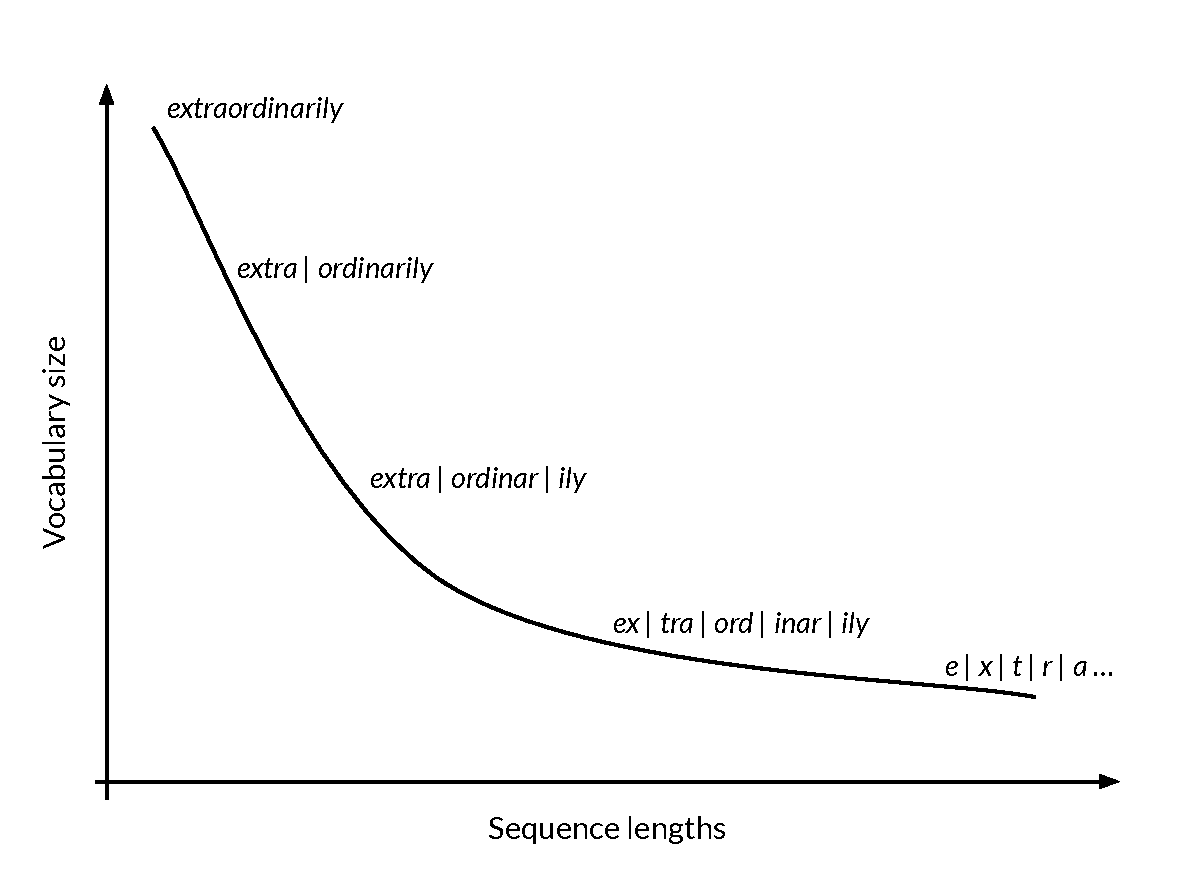
\includegraphics[width=0.5\linewidth]{sources/related_works/imgs/token_graph.pdf}
    \caption{}
    \label{fig:token_graph}
\end{figure}

Such statistical methods have dominated in the last few years as the default way to encode textual data, the most used being BPE \citep{sennrich-etal-2016-neural}, WordPiece \citep{wu2016google} and Unigram \citep{kudo-2018-subword}.

Byte-Pair Encoding, or BPE \citep{Gage1994bpe}, is a compression technique that relies on recursive symbol merges. In NLP, it is based on a dataset that consists in sequences of characters or bytes, and it iteratively registers a set of merge operations that reduce the count of merged items the most. WordPiece \citep{wu2016google} is based on a similar concept but uses a different rule for selecting merges. The possible merges $ab$ are scored according to:

$$
s(ab) = \frac{f_{ab}}{f_a \times f_b}
$$

where $f_{x}$ is the frequency of the string $x$ in the dataset. This scoring function differs from the basic BPE frequency as it favors merges $ab$ that appear in most cases when $a$ or $b$ appear. This typically leads to a more linguistically meaningful segmentation, as prefixes and suffixes are less prone to merging.

The Unigram tokenization algorithm \citep{kudo-2018-subword} works in the opposite direction : it first creates an exhaustive list of token candidates, and then iteratively removes tokens that affect the likelihood of the segmented sequence the least once discarded.

The statistical approaches are widely used in modern LMs, sometimes jointly with techniques such as subword regularization \citep{provilkov-etal-2020-bpe} that diversify segmentation results.

\paragraph*{Likelihood Maximization} Once the tokenization scheme is chosen, textual documents are parsed into sequences of tokens taken from a vocabulary of possible tokens  $\mathcal{V}$ of size $\left|\mathcal{V}\right| = V$. A \textit{training set} $T = (s_i)_{i\in[1, S]}$ of $S$ token sequences is thus built from the target textual documents. Each of these sequences $s_i$ has a given length $l_i$, and can also be written $s_i = (w_j)_{j \in [1, l_i]}$.

A language model $\phi_\theta$, based on a parameter set $\theta$, is a function that takes a sequence of tokens $\mathbf{w}_{\neq t}$ called context as an input, and outputs a probability distribution in $\Delta ^V$ for the token at position $t$.

The performance of a language model at token-level can be measured by computing the probability of the realization $w_t$ in the context $\mathbf{w}_{\neq t}$:
$$
\phi_\theta(\mathbf{w}_{\neq t})_{w_t} = P_\theta(w_t | \mathbf{w}_{\neq t})
$$

The process of training a language model consists in optimizing its average performance on the training set, which can be framed as a likelihood maximization objective \citep{mle}. In practice, to improve numerical stability, the objective is based on log-likelihood :
$$
\theta^* = \argmax_{\theta} E_T(\log \phi_\theta(\mathbf{w}_{\neq t})_{w_t})
$$

The minimized likelihood can also be seen as cross-entropy minimization between $P_\theta$ and an observed contextual probability distribution, estimated from the sample at position $t$, which is $\mathbf{1}_{w_t}$.

A metric that is often used to evaluate language modeling performance is \textit{perplexity} :
$$
\mathcal{P}(\phi_\theta, t) = 2^{-\log \phi_\theta(\mathbf{w}_{\neq t})_{w_t}}
$$


\subsection{Architectures}

\paragraph*{Statistical Methods}

The straightforward approach to language modeling consists in statistically estimating the distribution of tokens based on their context. 

In its most basic form, such statistical model estimates the \textit{unigram} distribution, that is the non-contextual distribution $P(w_t)$. This distribution is estimated by bin-counting tokens in the training dataset $T$ to retrieve token frequencies $f_w$ for each token $w$, and setting :
$$
\phi_{\theta}(\mathbf{w}_{\neq t}) = (f_w)_{w \in \mathcal{V}} \in \Delta^{V}
$$

We can extend this idea by estimating the \textit{2-gram} distribution $P(w_{t-1}w_t)$. To do so, we count the occurences of the subsequence $w_{-1} w_0$ in the training dataset for each pair of tokens $w_{-1}, w_0 \in \mathcal{V}^2$. Doing so, we can build a $V \times V$ stochastic matrix - i.e. which coefficients are non-negative reals that sum to $1$ column-wise - containing the observed frequencies for $w$ in pairs of the form $w_{-1} w$:
$$
M_2(T) = (f_{w_{-1} w})_{w_{-1}, w \in V^2}
$$
Then, the language model $\phi_{\theta}$ becomes:
$$
\phi_{\theta}(\mathbf{w}_{\neq t}) = (f_{w_{t-1} w})_{w \in V}
$$

More generally, $n$-gram language models \citep{jurafsky_course} can be designed to estimate the distribution $P(w_{t-n +1}...w_{t-1}w_t)$. By bin-counting $n$-uplet occurences in $T$, one can compute:
$$
M_n(T) = (f_{w_{-n+1}...w_{-1}w})_{(w_{-n+1}...w_{-1}), w \in V^{n-1} \times V}
$$
The associated language model $\phi_{\theta}$ can then be written:
$$
\phi_{\theta}(\mathbf{w}_{\neq t}) = (f_{w_{t-n+1}...w_{t-1} w})_{w \in V}
$$

These $n$-gram language models can be combined with backoff strategies to take sample size into accounts and switch between $n$ values when appropriate \citep{kneser_ney}.

\paragraph*{Neural Methods}
\citet{bengio2000neural} introduce the idea of training $\phi_\theta$ as a neural network with parameters $\theta$. The model is composed of three separate layers:

\begin{itemize}
    \item An \textbf{embedding} layer that corresponds to a look-up table that matches each token to a non-contextual feature vector that will be used as the input of the neural network;
    \item A hidden layer using a $\tanh$ non-linearity that maps the concatenation of $n$ input embeddings representing $w_{t-n+1}...w_{t-1}$ to an intermediate representation;
    \item An output layer that we call the \textbf{language modeling head} in reference to classification heads, that maps the intermediate representation to a $V$-dimensional vector.
\end{itemize}

\begin{figure}[h]
    \centering
    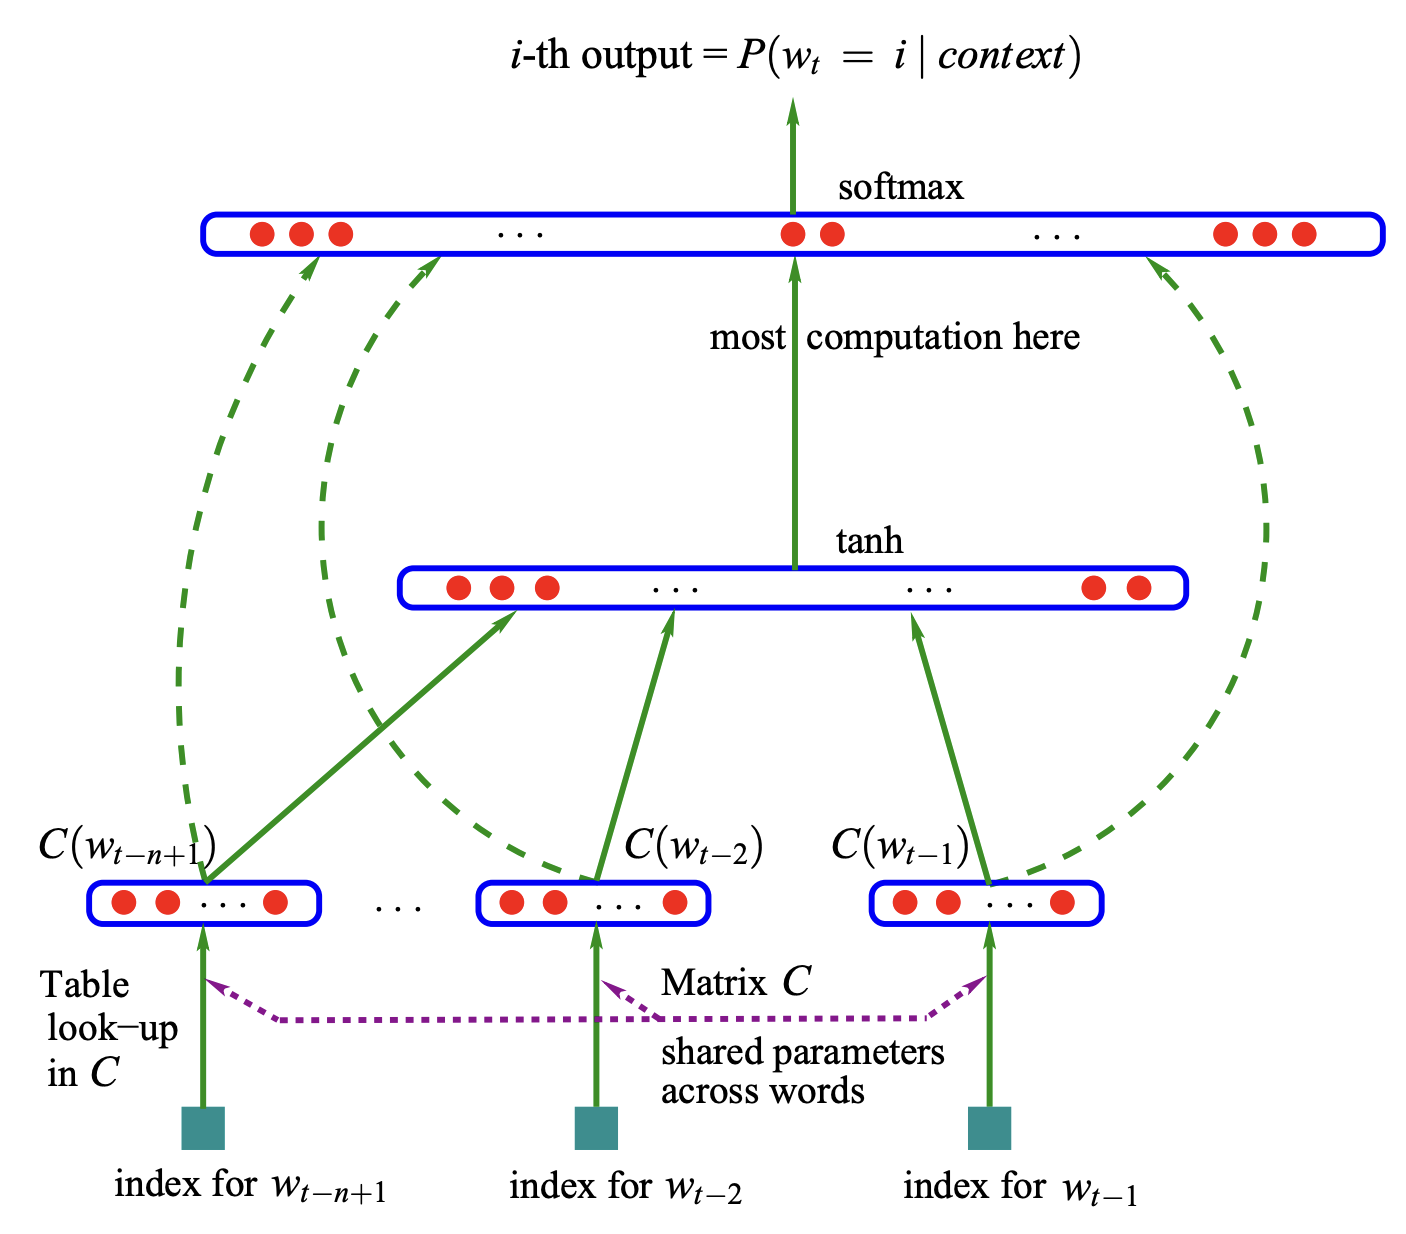
\includegraphics[width=0.5\linewidth]{sources/related_works/imgs/bengio_schema.png}
    \caption{Schema of a basic neural network architecture for language modeling (from \citet{bengio2000neural}).}
    \label{fig:bengio}
\end{figure}

The $V$-dimensional output is then normalized to a probability distribution using the softmax function. The softmax function $\zeta$ can be written component-wise for $x \in \mathbb{R}^d$ as :
$$
\zeta(x_i) = \frac{\exp(x_i)}{\sum_{j=1}^{d} \exp(x_j)}
$$

The model is then trained to optimize the log-likelihood using stochastic gradient descent (see \Cref{subsec:rl_optim}) on the parameters $\theta$ of the neural network.

\citet{bengio2000neural} train this neural architecture on the Brown corpus and the Associated Press News corpus and report substantial perplexity improvement compared with language models based on $n$-grams. This performance gap can be explained by the ability of neural networks to learn smooth contextual features, thus greatly improving extrapolation in the training feedback and at inference time.

A common trick that has been used in this framework is \textit{weight tying} \citep{press-wolf-2017-using}. It consists in using the same coefficients for the input embedding lookup table $W_{in} \in \mathbb{R}^{V \times d_m}$, and the language modeling head $W_{out} \in \mathbb{R}^{d_m \times V}$, by setting:
$$
W_{out} = W_{in}^T
$$
\citet{press-wolf-2017-using} show that this technique improves the performance of language models, while reducing their overall number of parameters.

\paragraph*{Recurrent Neural Networks}

A Recurrent Neural Networks (or \textit{RNN}) is a neural network that is trained to be applied sequentially to an input sequence, and that can use a past intermediate representation as input for present prediction. This concept was historically introduced in \citet{rnn_origins} but was first successfully applied to language modeling in \citet{mikolov10_interspeech}.

More precisely, input tokens are transformed into static embeddings using a similar look-up table as in \citet{bengio2000neural}, and a recurrent unit $\upsilon$ is then applied to the embedding sequence, sharing \textit{hidden states} $(h^1,...h^k)$ between each step of the sequential processing. The unit $\upsilon$ then processes the input embedding $x_t$ and the hidden states $(h_{t-1}^1,...h_{t-1}^k)$ at step $t$ through chosen tensor operations and non-linearities, returning an output representation $o_t$ in the process. The model can be described with this pattern:
$$
(o_{t}, (h_{t}^1,...h_{t}^k)) = \upsilon(x_t, (h_{t-1}^1,...h_{t-1}^k))
$$

Several variations have been proposed for this kind of models, notably improving the ability to avoid gradients issues related with the recurrence or to select information in the hidden states using specific functions in the unit. One of the most known variants is the Long Short-Term Memory (LSTM) unit introduced in \citet{HochSchm97} that has been widely used in NLP, including for language modeling \citep{miyamoto-cho-2016-gated}. The Gated Recurrent Unit (GRU) was later introduced in \citet{cho2014learningphraserepresentationsusing} as a simplification of the LSTM unit.

Although these units improve modeling abilities for long range dependencies \citep{rnn_eval}, they were empirically found to fail to handle interactions for elements separated by more than 1,000 time steps \citep{HochSchm97}.

\paragraph*{Transformers}

\citet{bahdanau_nmt} popularized the use of \textit{attention} in neural machine translation models as a method that lets the model select relevant tokens from the source sequence at a given prediction step. Such models, that previously used the last hidden states of a source-processing RNN (called \textit{encoder}) as the input to a target-generating RNN (called \textit{decoder}), suffered from an information bottleneck due to sharing only last-step representations between source and target sequences. The attention mechanism allowed to ease this bottleneck, by providing a \textit{direct path of interaction} between the source tokens and the decoder.

Attention was notably used in \citet{peters-etal-2018-deep} which use a bidirectional LSTM model for language modeling, before \textit{adapting} the model for downstream tasks, sometimes adding \textit{self-attention} layer (an attention mechanism that let a sequence interact with itself).

This idea was explored further in the notorious article \textit{Attention is All You Need} \citep{vaswani2017attention} that proposes to use attention as the only sequence-wise operation. As it is the main architecture that we will be using through our experiments, we proceed to thoroughly explain the inner workings of the Transformers block.

The original Transformers block or layer is a sequence processing block that mainly relies on Multi-Head Attention (or \textit{MHA}) to model inter-token interactions. The layer takes a sequence of $d_m$ dimensional representations $(x_t)_{t \in [1, L]}$ as an input, and outputs a similar sequence $(o_t)_{t \in [1, L]} \in \mathbb{R}^{L \times d_m}$. 

The input representations $x \in \mathbb{R}^{L \times d_m}$ are put through a multi-headed self-attention operation. More precisely, they are put through $3 \times n_h$ linear layers\footnote{For the sake of simplicity, we consider unbiased linear layers for the rest of this section.} with parameters $(W_Q^h, W_K^h, W_V^h)_{h \in [1, n_h]}$ of shape $d_m \times d_h$ where $n_h$ be the number of heads, and $d_h = \frac{d_m}{n_h}$. This constitutes three intermediate representations called queries $Q^h$, keys $K^h$, and values $V^h$ of shape $L \times d_h$:
\begin{equation*}
    \begin{cases}
        Q^h = x W_Q^h \\
        K^h = x W_K^h \\
        V^h = x W_V^h
    \end{cases}
\end{equation*}

Queries and keys are used to determine interaction weights between input representations via an attention map $A^h$ of shape $L \times L$, that is computed as:
$$
A^h = \text{softmax} \left(\frac{Q^h {K^h}^T}{\sqrt{d_h}}\right)
$$

The head-level output representations $v^h$ of shape $L \times d_h$ can then be understood as weighted sums of values based on the attention map rows:

$$
v^h = A^h V^h
$$

Finally, head-level representations are concatenated into the output representations of shape $L \times d_m$ and projected using a $d_m \times d_m$ linear layer of weights $W_o$:

$$
o = \text{concatenate}_{h\in [1, n_h]}(v^h) W_o
$$

This self-attention layer can be summarized in the following formula:
\begin{equation}
    \label{eq:self_attn}
o = \text{concatenate}_{h\in [1, n_h]} \left( \text{softmax} \left(\frac{x W_Q^h {W_K^h}^T x^T}{\sqrt{d_h}}\right) x W_V^h \right) W_o
\end{equation}


The authors argue that the main modeling improvement that this architecture yields is the direct cross-representation interactions that are allowed by the $Q^h {K^h}^T$ product, compared to the indirect interactions that are modeled in RNNs. Indeed, this matrix product can be decomposed into scalar products between queries and keys from different positions $i$ and $j$ in the sequence:

$$
(Q^h {K^h}^T)_{i, j} = \langle Q^h_i , K^h_j \rangle
$$

However, this modeling advantage comes at a quadratic cost in memory and time complexity, as the attention map needs to be computed using $O(L^2)$ operations, and stored using $O(L^2)$ floats. Variants propose to tackle this quadratic cost by restricting the $(i, j)$ position pairs where attention is computed, or by reducing the attention map size using various methods (see \Cref{subsec:efficient_attn}).

The expression of self-attention in \Cref{eq:self_attn} is non-causal, i.e. the output representation $o_t$ is a result of operations that can use input representations $x_t, x_{t+1}, ..., x_L$. For causal language modeling, where the used context should be $\mathbf{w}_{< t}$, the $o_t$ representation cannot be used for prediction at index $t + 1$ as it carries information from the future of the sequence, including $w_{t+1}$ through $x_{t+1}$. Hence, this architecture is not suited for a causal language model (or CLM) as such.

To account for causality in the self-attention operation, we can introduce a \textit{causal mask} $\mathcal{M}$ that will null out every non-causal interaction in the attention map, thus leading to $A^h_{ij} = 0$ when $i > j$. To do so, we instantiate $\mathcal{M}$ as:
\begin{equation*}
    \mathcal{M} = \begin{pmatrix}
        0 & -\infty & \cdots & -\infty \\
        \vdots & \ddots & \ddots & \vdots \\
        \vdots &  & \ddots & -\infty \\
        0 & \cdots & \cdots & 0

    \end{pmatrix}
\end{equation*}

We can then compute a causal self-attention map $A^h$ as:
$$
A^h = \text{softmax} \left(\frac{Q^h {K^h}^T}{\sqrt{d_h}} + \mathcal{M} \right)
$$

Now, $o_t$ only has access to representations $\mathbf{x}_{<t+1}$, and can directly be used for prediction at position $t+1$.

However, the Transformers block does not use the outputs of the self-attention operation directly, but rather surrounds the self-attention operation with highly-parameterized linear layers and normalizations. 

The representations $o$ are first summed with $x$ through a residual connection, which eases optimization and stabilizes gradients \citep{residual_conn}. The output is then regularized using layer normalization \citep{ba2016layernormalization}. Layer normalization is a form of representation regularization that avoids gradient-related issues due to the accumulation of layers. For a given set of representations $(e_t)_{t\in [1, L]}$, it performs the following normalization:
$$
\text{LayerNorm}(e_t)_i = \frac{e_{t, i} - \bar{e_t}}{\sqrt{\frac{1}{L} \sum_{j=1}^{L} (e_{t, j} - \bar{e_t})^2}} \times \gamma_i + \beta_i
$$

where $\bar{e_t}=\frac{1}{L} \sum_{j=1}^{L} e_{t, j}$ and $\gamma$ and $\beta$ are network parameters.

The Transformers block is then composed of a \textit{feed-forward} block, which is itself made of an upscaling linear layer of weights $W_{up} \in \mathbb{R}^{d_m \times d_{up}}$, an activation function and a downscaling linear layer of weights $W_{down} \in \mathbb{R}^{d_{up} \times d_m}$. A common choice for $d_{up}$ is $4 \cdot d_m$, and the activation function is typically one of ReLU \citep{relu}, GELU \citep{hendrycks2023gaussianerrorlinearunits} or SiLU \citep{silu}.

The last part of the block consists of another residual connection that adds the output of the first layer normalization to the output of the feed-forward layer, followed by a final layer normalization.

A Transformers model consists in a stack of Transformers block followed by a language modeling head of shape $d_m \times V$ that outputs logits $(l_t)_{t \in [1, L]}$. The Transformers causal language model $\phi_\theta$ for $t \in [2, L+1]$ can thus be written:

$$
\phi_\theta(\mathbf{w}_{<t}) = \text{softmax} (l_{t-1})
$$

Such a Transformers model based on causal self-attention is usually refered to as a decoder model, as it can be used as a decoder in a sequence-to-sequence model, in Machine Translation for instance. When causality does not matter for the targeted task, self-attention can be computed without the causality mask $\mathcal{M}$, which leads to an \textit{encoder} architecture.

In \citet{vaswani2017attention}, the main task is Neural Machine Translation, which leads to the use of an \textit{encoder-decoder} architecture. The source sequence is processed through an encoder Transformers, and the target sequence logits are generated using causal self-attention blocks with an added cross-attention layer. Cross-attention is similar to self-attention, but uses $Q^h$ and $K^h$ representations from one sequence and $V^h$ from another sequence. In the terms of \Cref{eq:self_attn}, cross-attention between sequences $x$ and $y$ can be written:

\begin{equation}
    \label{eq:causal_attn}
o = \text{concatenate}_{h\in [1, n_h]} \left( \text{softmax} \left(\frac{x W_Q^h {W_K^h}^T x^T}{\sqrt{d_h}}\right) y W_V^h \right) W_o
\end{equation}

A substantial difference between RNNs and Transformers is that positional information is not encoded naturally in the intermediate representations. Hence, several approaches have been introduced to embed positional information in Transformers models. These approaches can be split into two families: absolute positial embeddings (APE) and relative positional embeddings (RPE).

Absolute positional embeddings encode the position corresponding to the index of an item in the processed sequence. In \citet{vaswani2017attention}, the authors use sinusoidal functions to build representations of shape $d_m$ and add them to the input embeddings of the model. However, after \citet{devlin-etal-2019-bert}, the main approach has been to create a $L \times d_m$ lookup table of learnable parameters, and use row $i$ as a positional embedding for position $i$. The main limitation of such positional embeddings is that a model trained on sequences of length $L$ will be unable to process sequences of length longer than $L$, as no positional embeddings will be available for the additional positions.

Relative positional embeddings encode pairwise positional information in the self-attention map $A_h$ directly, and more specifically to the $Q^h {K^h}^T$ product. Usually, for a position pair $i, j$, RPE define functions $\omega_i$ and $\omega_j$, and a bias term $\beta_{ij}$:
\begin{equation}
    \label{eq:rpe}
(Q^h {K^h}^T)_{ij} = \langle \omega_i(Q^h_i), \omega_j(Q^h_j) \rangle + \beta_{ij}
\end{equation}

The most used RPE approaches are Rotary Positional Embeddings or RoPE \citep{rope}, and Attention with Linear Biases or ALiBi \citep{alibi}. In the framework of \Cref{eq:rpe}, RoPE can be expressed as:
$$
\begin{cases}
    \omega_i(x) = \mathbf{R^{d_m}_i}x \\
    \beta_{ij} = 0
\end{cases}
$$
where $\mathbf{R^{d_m}_i}$ is a rotary matrix that rotates pairs of dimensions with different angles depending on $i$. It can be written as the following blockwise diagonal matrix:
$$
\mathbf{R^{d_m}_i} = \begin{pmatrix}
    R_{i, \theta_1} & 0 & \cdots & 0 \\
    0 & \ddots & \ddots & \vdots \\
    \vdots & \ddots & \ddots & 0 \\
    0 & \cdots & 0 &  R_{i, \theta_{d_m/2}} \\
\end{pmatrix}
$$

where $R_{i, \theta} = \begin{pmatrix}
    \cos i \theta & -\sin i \theta \\
    \sin i \theta & \cos i \theta
\end{pmatrix}$ and $\theta_d = 10000^{\frac{-2(d-1)}{d_m}}$.

\citet{alibi} use a more straightforward approach. Their RPE, which relies on a linear bias on the whole attention map, can be written:
$$
\begin{cases}
    \omega_i(x) = x \\
    \beta_{ij} = m (i-j)
\end{cases}
$$
with $m \in \mathbb{R}$ as a head-specific fixed parameter.

\paragraph{Generation \& KV Cache}

Causal language models can be used for natural language generation, by sampling from the next-token probability and iterating over the sampled token or tokens. Although various generation strategies exist \citep{fan-etal-2018-hierarchical, wang2020contextual, nucleus_sampling}, the most straightforward one is greedy sampling, where the highest-probability next token is chosen and added to the generated sequence iteratively:
$$
w_{t+1} = \argmax_{w \in \mathcal{V}}\phi_{\theta}(\mathbf{w}_{<t+1})_w
$$

For RNNs, language generation is rather straightforward as the unit just requires the last hidden state and the current token input representation to make a prediction. For Transformers models however, a naive approach could consist in applying the model to the whole past sequence at each generation step, which would be $O(L^3)$ in time complexity. Luckily, the causal masking in self-attention implies that the post-attention representations $o$, which just depend on their own past, would be constant over generation steps, except for the last one $o_t$.

Hence, it is possible to cache the representations with indexes $i < t$ needed to generate $o_t$, which are $(K^h_i)_{i<t}$ and $(V^h_i)_{i<t}$. This caching technique is named KV caching.

\paragraph{Trained Models and Variants}
Highly influential Transformer-based language modeling works led to different model families : GPT \citep{Radford2018ImprovingLU}, BERT \citep{devlin-etal-2019-bert} and T5 \citep{2020t5}.

GPT (for \textit{Generative Pre-trained Transformer}) is a Transformers-based architecture that trains a decoder model for causal language modeling in a straightforward way. The training set is BookCorpus \citep{bookcorpus}, which contains unpublished books from a variety of genres. The authors use a 12-layer decoder-only Transformer with $d_m=768$, $n_h=12$ attention heads and a vocabulary of $V=40000$ tokens. Overall, GPT counts 110 million parameters.

GPT is used as a pre-trained model, and is thus fine-tuned for Natural Language Understanding downstream tasks from the GLUE benchmark \citep{wang-etal-2018-glue}. These tasks being mostly sentence-level classification tasks, the language modeling head of GPT is thus replaced with a pooling layer that extract a single representation from the output embeddings sequence by averaging or retaining the maximal value across hidden dimensions, followed by a classification head of shape $d_m \times n_c$ where $n_c$ is the number of classes for the target downstream task.

BERT (for \textit{Bidirectional Encoder Representations from Transformers}) is an encoder-only architecture trained for Masked Language Modeling or \textit{MLM}. A masked language model is a language model that uses the full context $\mathbf{w}_{\neq t}$ for the prediction at index $t$, which is called the masked token. In BERT, the authors propose to alter input token $w_t$ in the following way:
\begin{itemize}
    \item Replace it with a specific mask token 80\% of the time;
    \item Replace it with a random token 10\% of the time;
    \item Leave it unchanged 10\% of the time.\footnote{In that case, the training task is not language modeling but simply learning the identity mapping.}
\end{itemize}

In \citet{devlin-etal-2019-bert}, 15\% of the tokens are masked according to this procedure, and the cross-entropy training objective is used for the masked positions. By partially masking the whole sequence at once, the authors assume that altering one token does not hurt the feasability of the prediction at another position which uses this token in the context.
The original trained architecture is similar to GPT in parameter count and is similarly fine-tuned on downstream tasks, but a larger version is trained and achieves better performance. \citet{roberta} subsequently show that training on larger training sets leads to significantly better performance, and introduce the RoBERTa models suite.

T5 (for \textit{Text-to-Text Transfer Transformer}) is a model suite that aims for a different approach when it comes to downstream tasks. \citet{2020t5} argue that downstream tasks can be rephrased as natural language samples. For instance, the Corpus of Linguistic Acceptability, or CoLA \citep{warstadt2018neural} is a sentence-level classification task where a grammatical acceptability label (acceptable or unacceptable) is given to each sentence. The STSB subset of GLUE \citep{wang-etal-2018-glue} is a sentence-pair classification task where a similarity score in $[1, 5]$ is given to a pair of sentences. The authors argue that these tasks can be rephrased as language modeling tasks where the labels or scores are tokens that the model is expected to generate at inference time. The main advantage of this approach is that it does not require to have task-specific classification heads, which implies that the model can be fine-tuned on all tasks at once.

An optimized architecture for this task should be able to process an input sequence bidirectionally, and to generate a label for this input sequence. Thus, a natural choice is an encoder-decoder architecture, where the input sequence will be processed using the non-causal encoder, and a decoder using causal self-attention and cross-attention to the encoded sequence to generate the target label. \citet{2020t5} pretrain an encoder-decoder architecture for the language in-filling task, which extracts contiguous spans of tokens in the sequence, and trains a causal language model on these spans, using the rest of the sequence as the context. More formally, if the extracted span is $t_0, ..., t_0+\eta$, the T5 objective trains a causal language model on tokens $(w_i)_{i \in [t_0, t_0+\eta]}$ using context:
$$
\mathbf{w}_{\neq t} = (w_i)_{i \in [1, t] \cup ]t_0+\eta, L]}
$$

In T5, similarly to BERT, several spans are masked at once to avoid reprocessing the sequence, and under the assumption that it would maintain sufficient information to make convincing predictions. The authors release several models ranging from 60 million to 11 billion parameters for English language.

Following these works that mostly focus on English, several multilingual counterparts were released. Notable examples include mBERT, XLM-RoBERTa \citep{conneau2019unsupervised}, mGPT \citep{mgpt} or mT5 \citep{xue-etal-2021-mt5}.

\citet{electra} later notice that both GPT-like and BERT-like approaches are suboptimal when it comes to learning fine-tunable contextual representations using self-supervised methods. As a matter of fact, the contextual representations extracted from causal language models do not contain bidirectional information. On the other hand, only a fraction of the tokens are directly used when training masked language models, which may harm the data and compute efficiency of such an approach. \citet{electra} combine both these strenghts into the ELECTRA scheme: their pretraining approach directly uses every token available in each mini-batch, but also allows non-causal self-attention in the trained models. To that end, they use \textit{Replaced Token Detection} as a self-supervised task. They train two models: a smaller masked language model called the \textit{generator}, and a larger Transformers architecture called the \textit{discriminator}.

As in BERT \citep{devlin-etal-2019-bert}, a portion of the tokens is selected and used to pretrain the generator. The token associated with the highest predicted probability is then inserted at the selected position, and the resulting sequence is given as an input to the larger discriminator. The discriminator outputs a single float in $[0, 1]$ for each input token, which is trained to predict the probability that a position corresponds to a \textit{replaced} token, ie. a token that has been modified by the generator.

They conduct medium-scale experiments, training models ranging from 14M to 335M parameters, and observe that their pretrained models achieve parity with CLMs and MLMs when fine-tuned on downstream tasks, while using significantly less pretraining compute.


\paragraph*{Scale \& Performance}
The emergence of highly parameterized neural networks trained on large textual datasets as effective language models brings the question of scale, i.e. to what extent can scaling up either (or both) the volume of textual data or the count of trainable parameters can increase the language modeling performance and the downstream capabilities of models?

With RoBERTa \citep{roberta}, it appeared clear that the first generation of pretrained models, namely BERT and GPT, were undertrained. GPT-2 \citep{gpt2} is a follow-up model suite that was trained on a larger and more diverse dataset than BookCorpus called WebText, with model sizes ranging from 117 million to 1.5 billion parameters. The authors noticed that the larger GPT-2 models had interestingly better \textit{few-shot} and \textit{zero-shot} abilities, especially at question answering tasks.

GPT-3 \citep{gpt3} introduces a much larger architecture, using 175 billion parameters, while relying on a training procedure and architecture that do not significantly differ from the original Transformers-based GPT. The authors claim that this model displays a zero-shot downstream performance level that is close to fine-tuned counterparts. Similar results are reproduced through the OPT initiative \citep{zhang2022opt}. Subsequently, the 540 billion parameters PaLM model \citep{palm} was released, leading to similar conclusions. A multilingual counterpart to this line of work is BLOOM \citep{le2023bloom}, a 176 billion parameters model trained in 46 languages.

However well these models may perform, their training and inference raise a number of issues. Training these models consumes significant amounts of computational power, as it usually implies running thousands of Graphical Processing Units (GPUs) for multiple days, weeks or months. Moreover, these models are trained on enormous amounts of web-scraped textual data, which incentivizes the preparation of massive automatically cleaned textual datasets such as OSCAR \citep{oscar}, The Pile \citep{gao2020pile} or RedPajama \citep{together2023redpajama}. These datasets contain up to several trillions of tokens, which stands as a hard ceiling for language model training. Hence, it is both unclear whether it will be possible to train substantially larger language models on substantially larger text datasets, raising concerns about the possibility of a straightforward upscaling approach as a way forward for language modeling.

From the first Transformers-based models, the question of training optimal LMs under computational constraint has been considered in various ways. \citet{sanh2019distilbert} use knowledge distillation, i.e. using logits from a larger model as an objective for a smaller one, to train a smaller alternative to the base version of BERT that maintains a solid level of performance at reduced training and inference costs. \citet{turc2019} train a large set of small masked language models and show that pretraining student models before distillation leads to better performance. Other approaches have explored variants of knowledge distillation to improve performance for smaller models \citep{Fu_Zhou_Yang_Tang_Liu_Liu_Li_2021,sun-etal-2020-contrastive}.

A crucial result regarding the question of scaling is the empirical identification of \textit{scaling laws}, i.e. of explicit forms that accurately predict the final performance of a Transformers-based model based on $N$ non-embedding parameters and trained with a dataset composed of $D$ tokens. \citet{kaplan_scaling} are the first to discover this phenomenon, and they identify a scaling law that predicts the final cross-entropy loss $L(N, D)$ :
\begin{equation}
    \label{eq:kaplan}
L(N, D) = \left( \left(\frac{N_c}{N}\right)^{\frac{\alpha_N}{\alpha_D}} + \frac{D_c}{D}\right)^{\alpha_D}
\end{equation}
where $\alpha_N \approx 0.076$, $N_c \approx 8.8 \times 10^{13}$, $\alpha_D \approx 0.095$ and $D_c \approx 5.4 \times 10^{13}$ are empirically estimated parameters. \Cref{eq:kaplan} unsurprisingly predicts that LMs using more parameters or larger training datasets should have better language modeling performance. Moreover, it interestingly shows that for a fixed compute level $C \approx 6 N \cdot D$, there exist $N^*(C)$ and $D^*(C)$ that minimize $L$, so that training a larger model on less tokens or training a smaller model on more tokens both lead to poorer performance. Empirically, the values of $N^*(C)$ and $D^*(C)$ imply that the compute-optimal approach to language modeling consists in training relatively large models on small amounts of tokens.

However, \citet{chinchilla_scaling} suggest that the empirical results from \citet{kaplan_scaling} were not accurate. They first notice that \citet{kaplan_scaling} used intermediate checkpoints taken before complete cooldown, implying underestimated low-data performance. They also underline that there is a slight curvature of the scaling law by exploring larger model sizes to interpolate their scaling law. Their scaling law can be written:
\begin{equation}
    \label{eq:chinchilla}
    L(N, D) = \frac{A}{N^\alpha} + \frac{B}{D^\beta} + E
\end{equation}
where $A=406.4$, $B=410.7$, $\beta=0.28$, $\alpha=0.34$ and $E=1.69$.

Although the predicted pattern still implies that more parameters and/or training tokens lead to better log-likelihood levels, the values of $N^*(C)$ and $D^*(C)$ are leaning towards smaller models and larger amounts of tokens compared to \citet{kaplan_scaling}. Another notable difference is the introduction of a strictly positive limit to the loss when $N \rightarrow \infty$ and $D \rightarrow \infty$, which can be interpreted as the residual entropy of English language.

The scaling laws yield optimal $N$ and $D$ values for a fixed total training compute level $C$. However, they do not include inference computation cost in their equations, while it grows as the model size $N$ increases. \citet{beyond_chinchilla} take inference cost into account using \Cref{eq:chinchilla} and thus incentivize the training of even smaller models on larger datasets. Recent initiatives \citep{tinyllama,faysse2024croissantllm,gemmateam2024gemma} have followed this principle.

\subsection{Limitations \& Extensions}

\paragraph{The Softmax Bottleneck}

The concept of \textit{softmax bottleneck} was introduced in \citet{softmax_bottleneck}. In this article, the authors view the language modeling task through a matrix factorization prism. They decompose the language model $\phi_\theta$ into two parts : a model that outputs contextual embeddings $h_\theta(\mathbf{w}_{\neq t})$ of shape $d_m$, and a language modeling head $W_\theta \in \mathbb{R}^{d_m \times V}$:
$$
\phi_\theta(\mathbf{w}_{\neq t}) = \sigma (h_\theta(\mathbf{w}_{\neq t}) W_\theta)
$$

In a finite-length sequence framework, where possible contexts $\mathbf{w}_{\neq t}$ are countable, a contextual probability matrix can also be defined from the true distribution $P(w | \mathbf{w}_{\neq t})$:
$$
A = (\log P(w_i | c_j))_{i \in [1, V], j \in [1, C]}
$$
where $(c_j)_{j\in [1, C]}$ are the $C$ possible contexts.
Similarly, the language model can be described by the matrix:
$$
A_\theta = (\phi_\theta(c_j)_i)_{i \in [1, V], j \in [1, C]}
$$ 

The authors show that when $\rank A_\theta < \rank A$, which is likely when $d_m \ll V$, there exists contexts where the contextual probability distribution from $\phi_\theta$ cannot match the true distribution $P$.

They proceed to argue that $\rank A$ should be very high for natural language. In practice, measuring $\rank A$ would imply getting access to $A$ which is impossible. However, it can be argue that the distribution of tokens is highly context-dependent, as one single token (e.g. a negation marker) can imply a complete shift in token distribution at later positions. It is also unlikely that $\rank A$ is low as it does not seem plausible that only a few hundred of bases can express the whole diversity of contexts in language. These arguments hint towards higher rank values for $A$.

They propose to increase the possible rank of the language modeling head using a Mixture-of-Softmax. The language model is now decomposed into a first part that outputs $K$ contextual representations $h^k_\theta(\mathbf{w}_{\neq t})$ and a predicted mixture distribution $\pi_\theta(\mathbf{w}_{\neq t}) \in \Delta^K$ itself computed from hidden states through a softmax activation. The language model is then written:
$$
\phi_\theta(\mathbf{w}_{\neq t}) = \sum_{k=1}^K \pi_\theta(\mathbf{w}_{\neq t})_k \cdot \sigma (h^k_\theta(\mathbf{w}_{\neq t}) W_\theta)
$$

They argue that this Mixture-of-Softmax is more expressive that the vanilla approach, and provide experimental results in this direction.

Subsequent works have further explored the limitations of the softmax linear layer on language modeling performance, especially  \citep{chang-mccallum-2022-softmax} and other possible alternatives that rely on replacing the softmax layer with a more expressive counterpart \citep{lin2021breaking,sigsoftmax}. \citet{grivas-etal-2022-low} show that low-rank softmax layers can even lead to tokens that, although appearing in the training data, are never being predicted as the top-probability picks, and are thus never generated through greedy sampling.

\paragraph*{Tokenization}

Some of the induced biases of tokenizers can be harmful for modelization. One such limitation lies in their brittleness to character deformations which are commonly found in real world, noisy data. For instance, BERT's tokenizer~\cite{devlin-etal-2019-bert} encodes ``performance'' as \texttt{[``performance'']} but \mbox{``perfonmance''} as \texttt{[`per', `\#\#fo', `\#\#n', `\#\#man', `\#\#ce']}, which makes it hard for the model to behave similarly in both cases. Moreover, the tokenizer is fixed after its training and is therefore impossible to update without retraining, for instance to reflect new domains~\cite{el-boukkouri-etal-2020-characterbert} where tokenization might over-segment specific or technical terms. \citet{clark2022canine} list other issues emerging when using static subword tokenizers, especially when modeling languages with a more complex morphology than English.

Tokenizers are also a limitation when it comes to multilingual models. \citet{rust-etal-2021-good} show that training models using monolingual tokenizers systematically leads to better performance compared with multilingual ones. \citet{NEURIPS2023_74bb24dc} show that a single sentence can be 15 times shorter than its translation in another language. Moreover, the use of multilingual tokenizers often leads to the use of larger vocabularies which results in more weights being assigned to input embeddings. Nevertheless, \citet{liang2023xlmv} show that larger vocabularies lead to better downstream performance, thus indicating that multilingual models should ideally be able to handle such vocabularies at reduced cost.

\paragraph*{Character-level Models} Several alternative methods have been proposed to mitigate these tokenization issues.
This line-of-work suggests to learn character-level or byte-level representation for LMs instead of subword-level ones. These methods improve the robustness of LMs to naturally occurring noise as well as their expressiveness when dealing with out-of-domain or multilingual data. In order to cope with increased input lengths, some of these methods compress sequences with constant reduction rates obtained using specialized modules~\cite{clark2022canine,tay2021charformer}, subsequently removing any notion of subwords.

Some of the first neural networks for sequence generation used characters directly as inputs \citep{sutskever2011generating,graves2013generating}, and following works modified the approach to create input word representations based on characters \citep{kim2016character,Jzefowicz2016ExploringTL,peters-etal-2018-deep}. Similar architectures were recently adapted to work with Transformers. Notably, CharacterBERT \citep{el-boukkouri-etal-2020-characterbert} constructs whole word representations from character embeddings put through convolutions and highway layers, before feeding them to a Transformers architecture. \citet{ma-etal-2020-charbert} take this idea further by learning a BERT-style language model at character-level without intermediate pooling. 

Nevertheless, they still rely on fixed tokenization heuristics (for instance segmenting using whitespaces) which may not be suited to some languages or certain types of language variations. Several works have tried to remove these induced biases by working purely with characters or bytes as input. CANINE \citep{clark-etal-2022-canine} downsamples contextualized character representations via a strided convolution before feeding them to a Transformers. It can be trained either with a subword-based objective (CANINE-s) or with a character-level one (CANINE-c). \citet{tay2021charformer} design a similar model by replacing convolutions with efficient Transformers \citep{beltagy2020longformer}. A more direct approach, ByT5 \citep{xue-etal-2022-byt5} is a version of T5 that is trained at byte-level. Finally, \citet{yu2023megabyte} introduce the MEGABYTE model, by using a basic strided pooling approach to apply a Transformer architecture on $4$-bytes representations before using a more efficient model to decode these representations back to byte-level.

However, these methods either have to use various tricks to reduce the sequence lengths based on other induced biases like downsampling rates or have extremely low training and inference speeds \citep{xue2022byt5}. \citet{chung2016hierarchical} create tokens in a differentiable manner by predicting frontiers and using the representations of each character inside a ``token'', but it remains unclear how their model could be adapted to be used with newer architectures such as Transformers. \citet{mofijul2022vocabulary} propose to segment tokens using a trained ``frontier predictor.'' Nevertheless, this differentiable tokenizer is not trained with the main language model objective but instead mimics a BPE subword tokenizer, carrying some of its flaws.

Concurrently to this work, \citet{nawrot-etal-2023-efficient} propose to learn a dynamic tokenization scheme, using a module that predicts frontier positions and pools input bytes accordingly. They notably propose to use Gumbel noise \citep{gumbel-orig} through a sigmoid activation to sample a frontier decision variable in a differentiable manner. They proceed to train a differentiable tokenization scheme and succesfully reduce the perplexity and the latency of the language models on various languages.


\paragraph*{Efficient Self-Attention}

Self-attention has a quadratic complexity with respect to the sequence length $L$, as it requires the whole attention map $A \in \mathbb{R}^{L \times L}$ to be computed. In order to accelerate Transformers-based models, especially in long-context situations, several works have considered computing a subset only of the inter-positional interactions, or compressed versions of $A$. 

Notably, \citet{beltagy2020longformer} propose several alternatives in their Longformer architecture. First, they suggest only computing coefficients $(i, j)$ where $|i - j| < \delta$, thus resulting in a \textit{sliding window} pattern which gives its name to the method later used in Mistral models \citep{jiang2023mistral}. They proceed to present two variations of the sliding window attention: the first relies on a dilated pattern, and the second one allows a portion of the positions to use global attention, that is for a portion of $i$ values, the attention map value is computed at all positions $(i, j)$ for $j \in [1, L]$. These alternatives naturally come with their causal counterpart, for which the non-causal interactions are not included in the targeted  $(i, j)$ positions. The Longformer attention maps can be computed in $O(\delta L)$, which greatly accelerates inference in training when $\delta \ll L$.

The Linformer architecture \citep{wang2020linformer} takes a different direction and rather compresses $K^h$ and $V^h$ representations of shape $L \times d_h$ into representations of shape $k \times d_h$ using two $L \times k$ linear layers where $k \ll L$. The complexity of computing the self-attention maps becomes $O(k^2)$, allowing substantial acceleration at training and inference time. Similarly, \citet{nystromformer} use a Nyström decomposition of the attention map and achieve $O(L)$ complexity.

\paragraph*{KV Cache Compression}

As larger open-sourced models trained by industrial institutions emerged \citep{jiang2023mistral,touvron2023llama}, many efforts have aimed at improving the efficiency of self-attention as a \textit{post-training} step. This novel incentive paved the way for algorithms designed specifically for optimizing the attention maps of trained models. These algorithms usually avoid editing parameters of the model and are instead framed as \textit{KV cache compression}, as they indeed compress the cached $K^h$ and $V^h$ representations under language modeling performance constraints.

During generation, the KV cache grows linearly in size and it represents a total of :
$$
|KV|(t) = 2 d_h \times n_h \times t \times n_{lay}
$$
where $n_{lay}$ is the number of Transformer layers used in the model. Compressing the KV cache implies reducing the magnitude of one of these dependencies in order to overcome the memory limitations imposed by hardware constraint, notably when generating long sequences.

The dependency in $n_h$ can be reduced by using shared $K^h$ and $V^h$ representations across several heads. Multi-Query Attention or MQA \citep{shazeer2019fasttransformerdecodingwritehead} uses a single shared representation for a given position across all heads for a given layer. Grouped-Query Attention or GQA \citep{ainslie-etal-2023-gqa} takes a less radical stance, and shares $KV$ representations across $n_h / K$ heads, where $K$ is typically $4$ or $8$. The size of the KV cache is thus divided by $K$. Although \citet{ainslie-etal-2023-gqa} propose to shortly retrain an existing model that originally used regular MHA with GQA attention, \citet{touvron2023llama} successfully train models using GQA from scratch.

Substantial effort has been made in reducing the dependency of $|KV|$ in $t$, that is in shortening the sequences of KV representation at inference time. First, the previously discussed window attention \citep{beltagy2020longformer} can be seen as a KV cache compression method, as it corresponds to discarding the KV cache at positions before $t - \delta$. This method ensures that $|KV|$ is constant, but significantly hurts performance once $t > \delta$. \citet{xiao2024efficient} observe that the first tokens of a generated sequence are crucial along the whole generation and serve as \textit{attention sinks}. They propose a KV cache eviction scheme that only stores KV representations at indices $[1, s] \cup [t-\delta, t]$ where typically $s \in [1, 4]$. This allows to keep the attention sink positions in the cache, while retaining the constant size of the KV cache when $t > \delta$. They empirically show that this compression scheme is noticeably less harmful than window attention for downstream performance and long-context capabilities of resulting language models.

Concurrently to this line of work, other KV cache compression policies have chosen a different approach by building heuristics that dynamically determine whether a KV cache representation should be discarded or kept in memory. \citet{oren2024transformersmultistaternns} use the scalar products $\langle Q^h_t, K^h_i \rangle$ to discard the KV representations for position $i$ where this score is lowest at generation step $t$. \citet{h2o} computes cumulated normalized attention scores for each position in order to decide which representations to discard. \citet{keyformer} notice that tokens for which attention scores are low actually help regularize the higher attention scores at preserved positions. As a result, removing these low-attention representations disturbs the nature of the attention map. They suggest a smoothing technique that mitigate this issue and improve the performance of the compressed models.

These dynamic compression policies \citep{shi2024costdownreviewmethods} are heuristics and may suboptimal as such. \citet{nawrot2024dynamic} propose a differentiable KV cache compression scheme that can be added to a trained model and optimized to minimize $|KV|$ while retaining the language modeling performance. They suggest using the first component of $K^h_t$ representations as an input signal for a Gumbel-Sigmoid that predicts the creation of a new slot in the KV cache. If the output of the Gumbel-Sigmoid is $1$, $K^h_t$ and $V^h_t$ are merged with their last counterparts in the compressed KV cache through a weighted average. Else, if the output is $0$, a new position is allowed in the KV cache and initialized with $K^h_t$ and $V^h_t$. Thanks to the Gumbel reparameterization trick \citep{gumbel-orig}, this scheme is differentiable, and the compression ratio can be measured by averaging the outputs of the Gumbel-Sigmoid. This compression ratio is thus differentiable and can be considered as an auxiliary loss for the language model during retraining.




\paragraph*{Biases \& Ethical Concerns}

\citet{parrots_bender} notoriously present issues related with the increasing scale of language models. They argue that, as language models grow larger and more performant, their financial and ecological costs should be considered as a potential concern in the long run, as has been explored in other works \citep{su14095172, rillig_2023}. They add that these commercial large language models (or LLMs) being trained on large web-scraped datasets that are poorly curated, they may contain dangerous and socio-culturally biased information that is then reproduced by the model at inference. These biases may include sterotypical views about gender \citep{kotek2023gender}, religious groups \citep{10.1145/3461702.3462624} or race \citep{nadeem-etal-2021-stereoset}, among others.

\newpage





%%%%%%%%%%%%%%%%%%%%%%%%%%%%%%%%%%%%%%%%%%%%%%%%%%%%%%%%%%%%%%%%%%%%%%%%
\section{Representation Learning}
%%%%%%%%%%%%%%%%%%%%%%%%%%%%%%%%%%%%%%%%%%%%%%%%%%%%%%%%%%%%%%%%%%%%%%%%
\begin{center}
  \begin{minipage}{0.5\textwidth}
    \begin{small}
      In which the reasons for creating this package are laid bare for the
      whole world to see and we encounter some usage guidelines.
    \end{small}
  \end{minipage}
  \vspace{0.5cm}
\end{center}

\subsection{Introduction}


%%%%%%%%%%%%%%%%%%%%%%%%%%%%%%%%%%%%%%%%%%%%%%%%%%%%%%%%%%%%%%%%%%%%%%%%
\subsection{Statistical approaches}
%%%%%%%%%%%%%%%%%%%%%%%%%%%%%%%%%%%%%%%%%%%%%%%%%%%%%%%%%%%%%%%%%%%%%%%%
Statistical approaches to representation learning primarily involve methods that leverage co-occurrence statistics and distributional properties of words. Key techniques in this category include:

\begin{itemize}
  \item Latent Semantic Analysis (LSA): LSA is based on the Singular Value Decomposition (SVD) of term-document matrices, reducing the dimensionality of the data and uncovering latent semantic structures. By mapping words and documents to a shared vector space, LSA captures semantic similarities based on co-occurrence patterns.
\end{itemize}


Latent Dirichlet Allocation (LDA): LDA is a generative probabilistic model that represents documents as mixtures of topics, where each topic is a distribution over words. By inferring the topic distribution for each document, LDA provides a way to represent documents in a lower-dimensional topic space.

Word2Vec: Introduced by Mikolov et al., Word2Vec includes two model architectures—Continuous Bag of Words (CBOW) and Skip-gram. These models learn word embeddings by predicting the context words surrounding a target word or vice versa. The resulting vectors capture semantic relationships such as analogies (e.g., "king" - "man" + "woman" $\simeq$ "queen").

GloVe (Global Vectors for Word Representation): GloVe is another word embedding technique that combines the advantages of matrix factorization and local context window methods. It constructs a word-word co-occurrence matrix and derives word vectors by factorizing this matrix, ensuring that the dot product of word vectors approximates the logarithm of their co-occurrence probabilities.

%%%%%%%%%%%%%%%%%%%%%%%%%%%%%%%%%%%%%%%%%%%%%%%%%%%%%%%%%%%%%%%%%%%%%%%%
\subsection{Auto-encoders}
%%%%%%%%%%%%%%%%%%%%%%%%%%%%%%%%%%%%%%%%%%%%%%%%%%%%%%%%%%%%%%%%%%%%%%%%
Auto-encoders are neural network models designed to learn efficient representations of data through unsupervised learning. They consist of an encoder that maps input data to a latent space and a decoder that reconstructs the original data from this latent representation. In NLP, auto-encoders can be used to learn embeddings for words, sentences, or documents.

Basic Auto-Encoders: The simplest form of auto-encoders involves a single hidden layer that compresses the input into a lower-dimensional latent space. The model is trained to minimize the reconstruction error between the input and the output.

Variational Auto-Encoders (VAEs): VAEs extend basic auto-encoders by imposing a probabilistic structure on the latent space. They use a probabilistic encoder to map inputs to a distribution in the latent space, allowing for the generation of new samples by sampling from this distribution. VAEs are useful in tasks requiring generative capabilities, such as text generation.

Denoising Auto-Encoders (DAEs): DAEs are trained to reconstruct the original data from corrupted versions. This process encourages the model to learn robust features that are invariant to noise, improving the quality of the learned representations.

\subsection{Contrastive approaches}

Contrastive approaches in representation learning aim to learn effective embeddings by contrasting positive and negative examples. The core idea is to bring similar items closer together in the embedding space while pushing dissimilar items apart. These methods are essential for capturing nuanced relationships in the data and enhancing the quality of learned representations.
\begin{itemize}
  \item Contrastive Loss: The fundamental concept in contrastive learning is the contrastive loss function, which drives the learning process by encouraging the model to distinguish between positive pairs (similar items) and negative pairs (dissimilar items).
  \item Triplet Loss: Triplet loss is a popular contrastive learning technique that uses triplets of samples: an anchor, a positive (similar to the anchor), and a negative (dissimilar to the anchor). The objective is to minimize the distance between the anchor and the positive while maximizing the distance between the anchor and the negative. This approach is widely used in tasks such as face recognition and text similarity.
  \item 
  Noise Contrastive Estimation (NCE): NCE is another contrastive learning method that reformulates the problem of estimating a probability distribution into a binary classification problem. The model learns to distinguish between observed data and artificially generated noise samples. NCE is particularly useful in large-scale language models where direct computation of probabilities is computationally expensive.
\end{itemize}

%%%%%%%%%%%%%%%%%%%%%%%%%%%%%%%%%%%%%%%%%%%%%%%%%%%%%%%%%%%%%%%%%%%%%%%%
\chapter{Representation Analysis for NLP}
\label{chap:rw_repr_ana}

%%%%%%%%%%%%%%%%%%%%%%%%%%%%%%%%%%%%%%%%%%%%%%%%%%%%%%%%%%%%%%%%%%%%%%%%
With the advent of neural methods for NLP systems, it became significantly more difficult to explicitly and totally control the inner behavior of the model, which was straightforward in \textit{symbolic} methods, as well as in purely statistical ones, to a certain extent. 

Analyzing the weights and activations of the intermediate layers of neural NLP models is the purpose of the \textit{interpretability} field \citep{interpretability_survey}. In this section, we briefly depict interpretability methods, with a particular focus on works that describe the intermediate vector spaces. We also present some methods that are directly derived from these observations.

\section{Representations and Embedded Knowledge}
In this first section, we consider approaches that view language models as grey-box systems, and identify properties of layer-wise intermediate representations without deep-diving into the underlying architectures.

\subsection{Linear Representation Hypothesis}

\begin{figure}[ht]
    \centering
    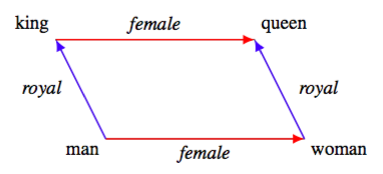
\includegraphics[width=0.5\linewidth]{sources/related_works/imgs/parallelograms_kawin.png}
    \caption{Illustration of the linear representation hypothesis as mentioned in \citet{mikolov-etal-2013-linguistic} (taken from \citet{ethayarajh-etal-2019-towards})}
    \label{fig:parallelo}
\end{figure}

A fundamental concept in neural model interpretability (and particularly for language models) is the linear representation hypothesis, i.e. the observation that \textit{high-level concepts are represented linearly as directions in [the] representation space} \citep{park2024the}.

This hypothesis was famously invoked in the Word2Vec article\footnote{The claim is usually attributed to Word2Vec but was initially made in an article from the same first author.} \citep{mikolov-etal-2013-linguistic}, where authors argued that arithmetic operations between the representations almost perfectly captured semantic relationships. For instance, they have been shown to capture analogies, as in the notorious example:
$$
x_{\text{queen}} \simeq x_{\text{king}} - x_{\text{man}} + x_{\text{woman}}
$$

This observation was explored and justified mathematically in the context of static word embeddings \citep{ethayarajh-etal-2019-towards, pmlr-v97-allen19a}. Recently, \citet{jiang2024on} showed that training a probabilistic model by optimizing cross-entropy via gradient descent theoretically pushes for a linear representation of underlying concepts, which generalizes the mathematical grounding of this hypothesis to representations of neural LMs. 

Most importantly, the linear representation hypothesis implies that self-supervised neural models can be \textit{probed} using linear methods in order to measure the extent to which a given concept is embedded in their representations. 

Typically, given $d$-dimensional frozen hidden representations modeled by a random variable $h$ and associated labels (respectively values) $y$ corresponding to a given concept, the \textit{linear probing} technique amounts to optimizing a linear (or affine) model $f_\Psi$ for a classification (respectively regression) loss $l$, i.e.:
$$
\Psi^* = \argmin_{\Psi} \mathbf{E}_{h, y}(l(f_\Psi(h), y))
$$

The resulting performance of the probe $f_\Psi$ indicates to what extent the representations encode the given concept. For instance, $h$ could encode sentence embeddings and $y$ could be a gender label for the subject in the sentence. Then, $l$ will be a classification loss, and $f_\Psi$ a trainable mapping from a representation $h_i$ to a gender prediction $\hat{y}_i$. In this example, he performance of the probe would indicate the amount of gender-related information that is encoded in the sentence representations.

\subsection{Embedded linguistic properties}
\begin{figure}[ht]
    \centering
    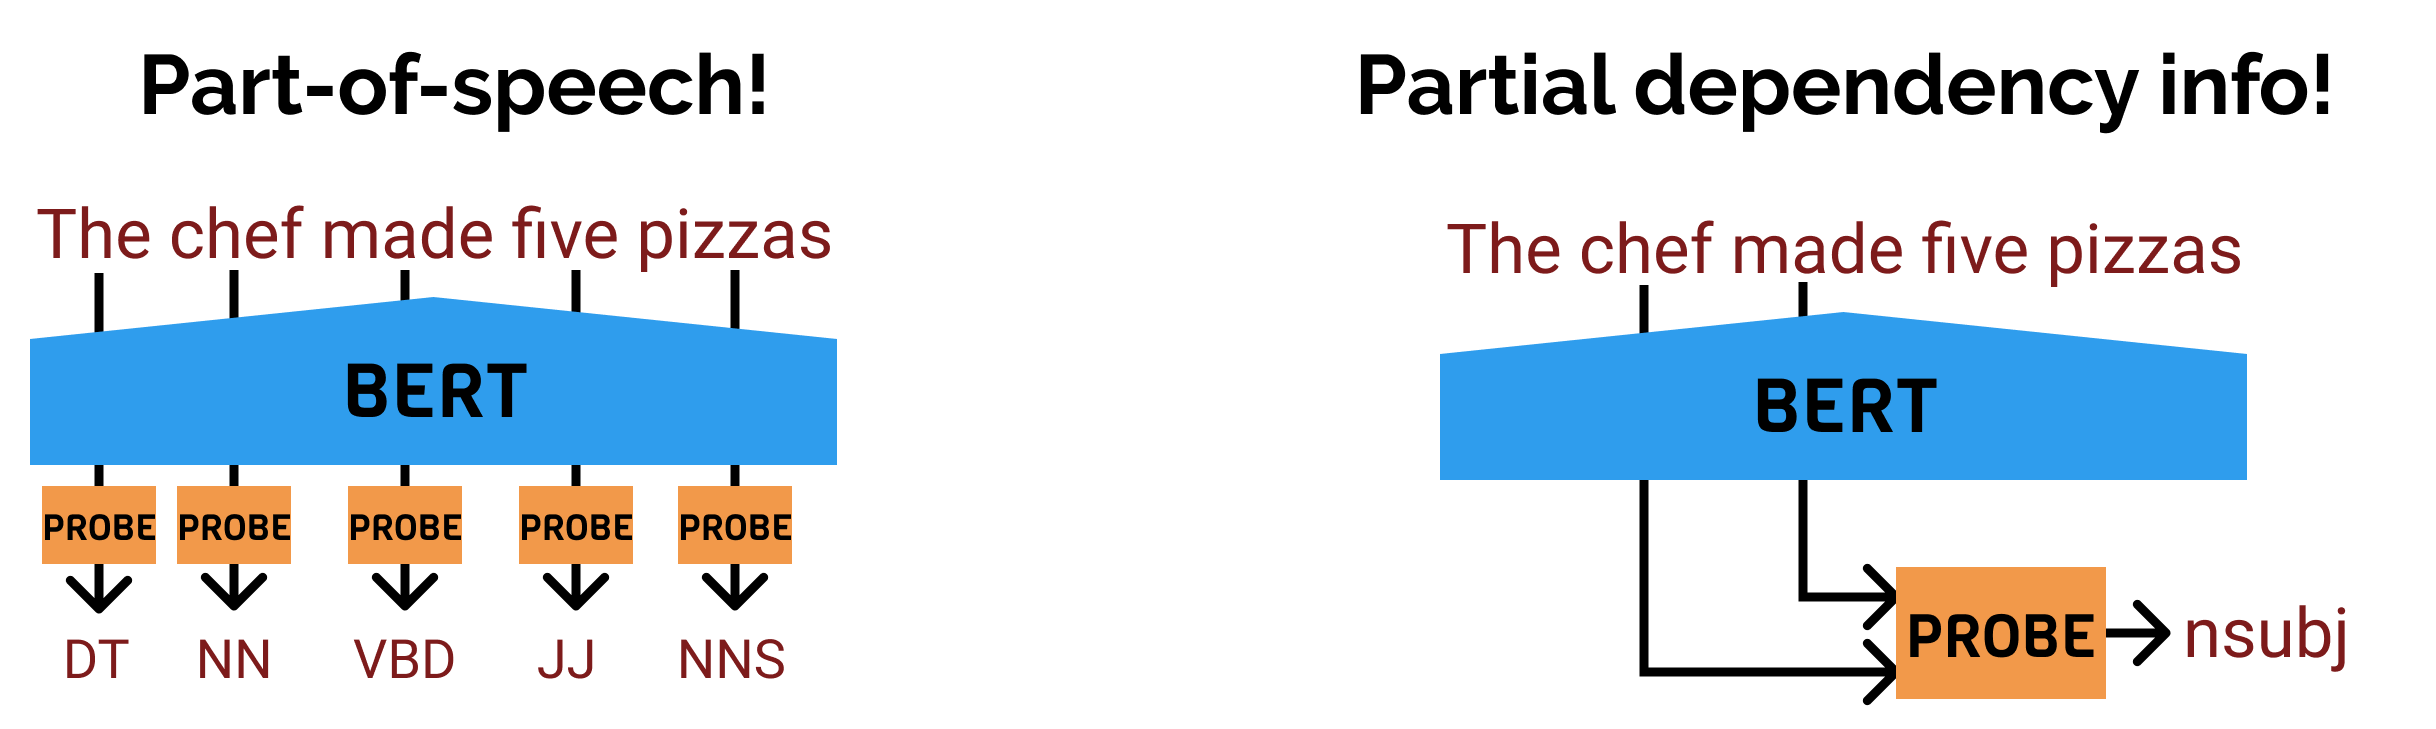
\includegraphics[width=0.7\linewidth]{sources/related_works/imgs/probing-diagram.png}
    \caption{A high-level summary of probing for language models (taken from \citet{Hewitt_2019})}
    \label{fig:probing}
\end{figure}



Early in the development of neural embedding methods, probing has been implemented to improve the understanding of how the representations capture information. \citet{kohn-2015-whats} successfully probe Word2Vec embeddings for basic word-level linguistic properties such as Part-of-Speech or gender. \citet{shi-etal-2016-string} show that RNN-based machine translation models partly learn the syntax of the source language using probing. \citet{adi2017finegrained} and \citet{conneau-etal-2018-cram} probe sentence representations from a linguistical point of view. They focus on relatively basic properties, such as the sentence length, or the belonging of a given token. \citet{liu-etal-2019-linguistic} extend this idea to token-level representations, and propose to use usual downstream tasks, such as POS tagging or Named Entity Recognition, as probing tasks. They train layer-wise probes and show that the necessary linguistic information is better contained in deeper layers.

These probing tasks have been used to better understand the layer-wise organization of neural LMs. \citet{peters-etal-2018-dissecting} show that the first layers focus on local syntax, while deeper layers focus on semantic content. \citet{tenney-etal-2019-bert} further decompose the roles of layers and find that the BERT model unsupervisedly mimics traditional NLP pipelines, i.e. it first latently parses the sentences before identifying coreferences and semantic relations. \citet{jawahar-etal-2019-bert} come to similar conclusions, but also notice that BERT is able to capture linguistic hierarchy and to mimic tree-like structures at representation level.



\subsection{Embedded world knowledge}


Several works have probed models in search for world knowledge, in order to quantify the ability of LMs to learn meaningful representations of physical objects beyond linguistic semantic.

\citet{gupta-etal-2015-distributional} show that static representations contain referential information about named entities. For instance, it is possible to roughly estimate population count, geolocation and other properties from city or country names using a basic probe.

Subsequently, different works have studied temporal knowledge \citep{thukral-etal-2021-probing, caselli-etal-2022-time}, auditive representations \citep{ngo2024languagemodelshearprobing} or factual knowledge \citep{youssef-etal-2023-give}, among others. In this work, we focus on geographical knowledge, and wonder whether geo-localisation information is embedded in the representations of geographical entities.

\citet{lotr} show that coordinates of places in the Middle-Earth can be predicted by just using the co-occurence matrix extracted from the Lord of the Rings novels. \citet{faisal-anastasopoulos-2022-geographic} build networks from geographical representations based on monolingual and multilingual models of different sizes. They show that all models embed more accurate geographical representations for countries of the Global North. This geographical discrepancy can be explained by biases that are inherent to the datasets used for pretraining \citet{faisal-etal-2022-dataset}.

Recently, \citet{gurnee2023language} probed large language models from the Llama-2 suite \citep{touvron2023llama} to extract coordinates of prompted locations from hidden representations across layers. They show that models ranging from 7B to 70B parameters are able to convincingly embed geographical coordinates on a world map when representing basic prompts. They prove that scaling up the model size systematically leads to better performance in coordinates prediction.

\citet{peters-etal-2019-knowledge} propose to use the probe loss as an auxiliary objective during training, explicitly encoding chosen properties in the representations. They argue that the resulting model is more performant on downstream tasks after fine-tuning.

A concurrent line-of-work rather focuses on the analysis of data-inherent socio-cultural biases in models at representation-level. Instead of probing encyclopedic world knowledge, these methods evaluate the extent to which language models are contaminated by the stereotypical views that belong in natural language, or by statistical imbalances that may implicitly reinforce these views in these models.

\citet{zhao-etal-2018-gender} study gender bias in co-reference resolution systems. Co-reference resolution is a linguistic task that consists in indentifying the object of a reference (a pronoun referring to a past name for instance) that could potentially seem ambiguous. Analyzing the errors made by a coreference resolution system can provide insights about its underlying representations of concepts. For instance, let us consider the sentence ``\textit{the physician hired the secretary because she was overwhelmed with clients}''. A model that wrongly predicts that \textit{she} refers to \textit{secretary}, but would predict the correct reference when replacing \textit{she} with \textit{he}, likely suffers from stereotypical gender biases. They propose to quantify gender bias more directly in static embeddings by measuring the cosine similarity between the gender token (e.g. \textit{female}) and attributes like profession tokens (e.g. \textit{colonel}) \citep{zhao-etal-2018-learning}.

\citet{zhao-etal-2018-learning} go further and introduce auxiliary objectives to the GloVe method that help minimize their bias metric, which implies minimizing the alignment between some attributes and gender in the token-level representation space. In a similar effort, \citet{ravfogel-etal-2020-null} post-edit statistical embeddings by iteratively projecting them on the orthogonal direction of a trained linear probe. Intuitively, training a new probe on these projected embeddings should be more difficult as a gender-sensitive direction has been suppressed from the latent space. \citet{iskander-etal-2023-shielded} extend this idea to more complex probes and introduce a gradient-based method of which \citet{ravfogel-etal-2020-null} is a particular case.





\section{Analysis of Self-Attention}

After the emergence of Transformer-based models, many interpretability works have focused on the multi-head self-attention layers. These layers differ from the other linear layers as they model the interactions between tokens.

\subsection{Properties of self-attention maps}

When attention was introduced as a way to improve machine translation neural systems \citep{bahdanau_nmt}, it was shown that cross-attention maps were implicitly modeling token-to-token cross-lingual mappings. 

The self-attention patterns of BERT have been analyzed in numerous works. \citet{clark-etal-2019-bert} describe head-specific patterns, such as attending to punctuation, special tokens used for self-supervision (e.g. \texttt{[SEP]} or \texttt{[CLS]}), and previous or next tokens. They also identify a pattern with the entropy of head-level attention maps, where lower layers contain high-entropy maps that roughly average the representations of all token positions. They proceed by identifying specific heads that specialize in extracting a specific type of linguistic phenomenon through attention maps. They use attention maps and GloVe embeddings as an input to a dependency parsing classifier, and obtain satisfying results, showing that attention maps latently perform operations that are related with parsing.

\citet{voita-etal-2019-analyzing} conduct a similar analysis and find that pruning non-specialized heads does not significatively affect performance in Transformer-based machine translation. \citet{vig-belinkov-2019-analyzing} concurrently identify head-specific patterns on GPT-2 \citep{gpt2}, and add that deeper layers tend to encode longer-term dependencies than first layers.

Overall, these works show that self-attention maps in language models tend to be sparse (or low-entropy), which can make them easily interpretable in some cases. Quantitavely, head-level probing tasks and downstream evaluation allows to measure and characterize their specialization from a linguistic point of view.

\subsection{The logit lens}

\begin{figure}[ht]
    \centering
    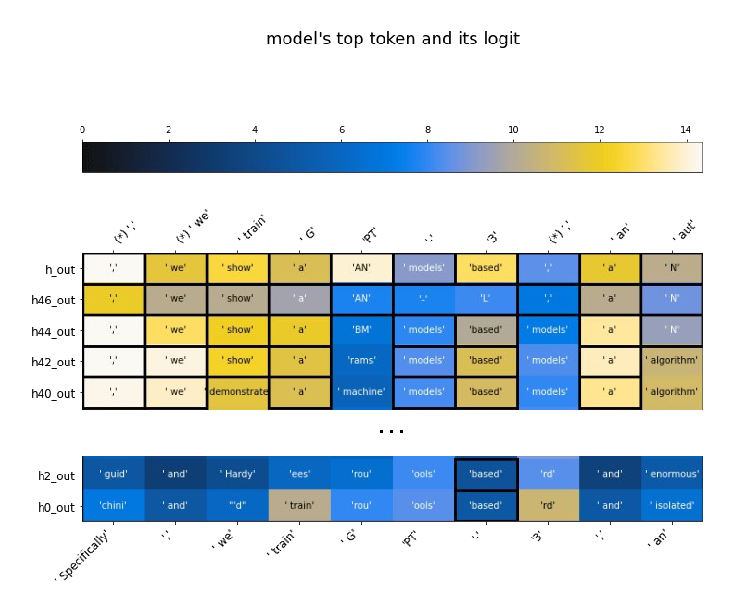
\includegraphics[width=0.7\linewidth]{sources/related_works/imgs/logit_lens.pdf}
    \caption{Layer-wise diagram obtained with the logit lens technique (taken from \citet{logit_lens})}
    \label{fig:logit_lens}
\end{figure}

Although the methods mentioned above are efficient at measuring the quantitative linguistic performance of specific parts of Transformer models, they depend on a biased evaluation protocol, as the tasks and measurements are made with a specific angle of study. This remark led to the elaboration of techniques that automatically discover interpretable patterns.

\citet{logit_lens} introduce the concept of \textit{logit lens} \citep{logit_lens}, a projection technique that allows to extract token-related interpretations from intermediate representations in Transformer blocks. They observe that the residual connections of Transformer architectures create direct paths to the last hidden representation, which is then simply projected linearly on a $V$ dimensional logit space by the language modeling head. Hence, they hypothesize that the structures of the representations that go through these residual connections are suited for the language modeling head, implying that projecting them through this layer will produce meaningful outputs in the logit space. They mostly use this observation to analyze the stacked layers as improving predictors and to display their intermediate predictions.

\citet{elhage2021mathematical} develop a more elaborate framework around a similar idea, and identify \textit{circuits} in Transformer models, i.e. paths through the layers via a residual stream that processes specific features with each linear operation

\citet{prakash-lee-2023-layered} use the logit lens technique on large LMs to investigate the semantic changes that occur after bias mitigation techniques \citep{ravfogel-etal-2020-null}. \citet{dar-etal-2023-analyzing} design an equivalent framework to analyze model weights in the token space.

These initiatives tend to show that Transformer layers all contribute to the final prediction through a residual stream, where some heads sparsely process input representations in an interpretable way. Once more, these sparse implicit operations happen in linear subspaces that can be analyzed in token space via basic operations.

\subsection{QKV geometry}
To the best of our knowledge, few works have specifically studied the vector distributions of attention-level representations $Q^h$, $K^h$ and $V^h$.

Recently, \citet{devoto2024simpleeffectivel2normbased} observed that the $L_2$ norm of the $K^h$ representations could be used as a proxy for subsequent attention weights. They derive an efficient KV cache compression scheme from this observation, proving that $K^h$ representations with the highest $L_2$ norm can actually be discarded at inference time without significant performance loss.

\section{Representation degeneration}
\label{sec:rw_degeneration}

Representation Degeneration is a phenomenon in which pretrained models tend to adopt low-entropy singular value distributions \citep{jing2022understanding}. In other words, the singular value distributions of the representations of affected models are particularly imbalanced, which implies that they can be efficiently approximated in a lower-dimensional subspace.

In language modeling, representation degeneration has been studied from various points of view, and specificities related to the (Zipfian) distribution of textual data have been put forward to explain the forms of degeneration that were observed at various levels in models. Hence, we argue that representation degeneration can be included in the field of interpretability, as it depicts distortions that may be explained by general properties of natural language.

We summarize the works that cope with this question in the following sections.

\subsection{A general phenomenon}

\citet{9709917} identify dimensional collapse as a potential caveat of self-supervised models in general. They suggest that features tend to naturally collapse towards highly dependent patterns. To measure this phenomenon, they track several metrics for the generated representations. They estimate the rank of the space spanned by the representations by computing the singular values of a representation set, and show that this estimated rank tends to decrease in training. They also measure the average absolute correlation scores across features, and show that this correlation does not naturally decrease. 

A way to circumvent this phenomenon is to penalize feature similitude, which they implement through a covariance regularization term. \citet{pmlr-v139-tian21a} show that architectural tricks such as weight decay \citep{weight_decay} or exponential moving averaging \citep{morales-brotons2024exponential} can mitigate dimensional collapse.

Another natural approach towards mitigating dimensional collapse is contrastive learning, as it implicitly improves the uniformity of latent spaces \citep{pmlr-v119-wang20k}. Nevertheless, \citet{jing2022understanding} show that for a broad range of data augmentation techniques used when generating positive samples, contrastive methods lead to dimensional collapse. They design architectural tricks and improved data augmentation methods to alleviate this issue.

Most importantly, in agreement with \citet{pmlr-v119-wang20k}, these works notice that uniformity in latent spaces is correlated with performance, and that mitigating dimensional collapse leads to better models in general.

\subsection{Degeneration in NLP}
\label{ssec:degeneration}

\begin{figure}[ht]
    \centering
    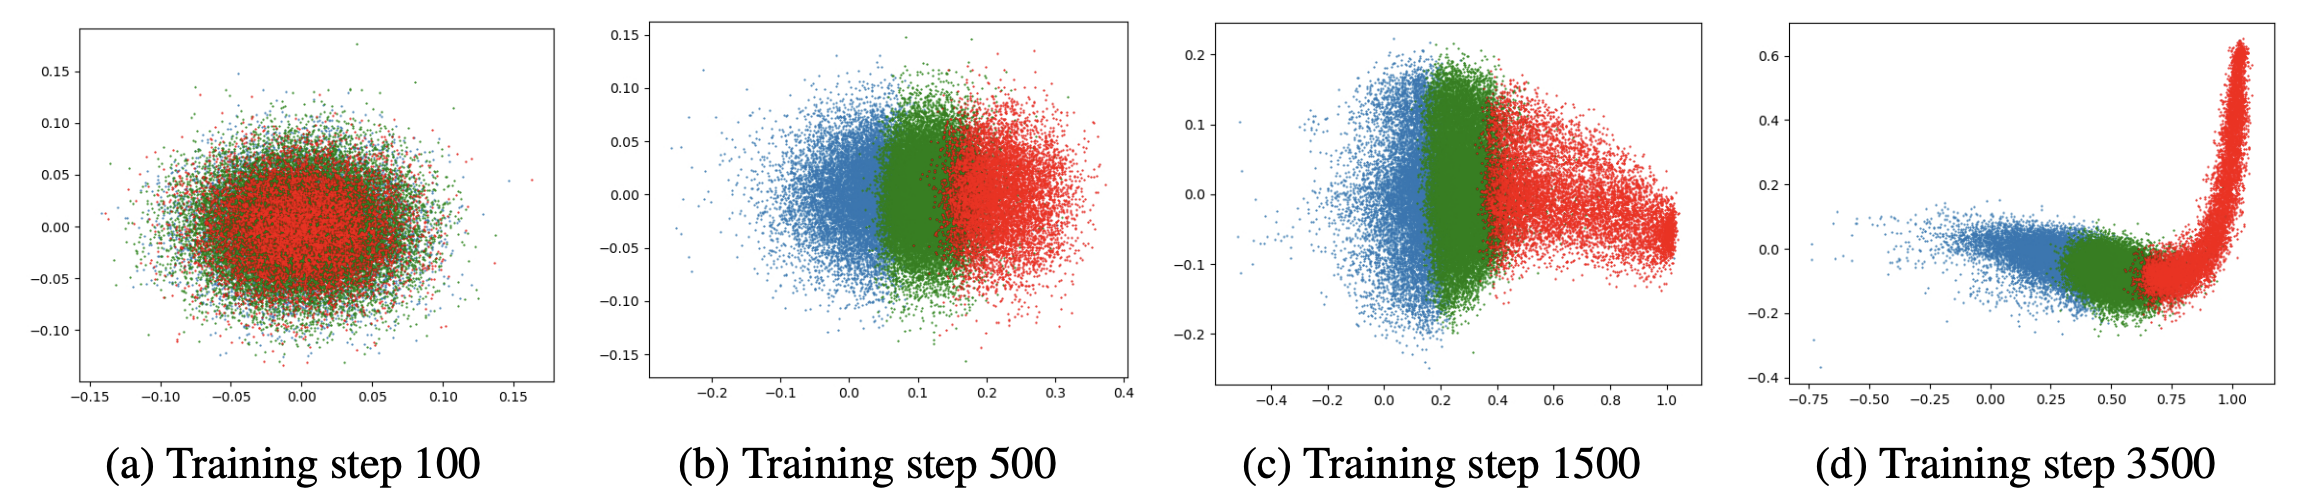
\includegraphics[width=0.9\linewidth]{sources/related_works/imgs/freq_degen.png}
    \caption{Visualization of the token embeddings of a language model during training, projected onto the first two components of their SVD. Red, green, and blue points represent rare, medium, and frequent groups respectively (taken from \citet{yu-etal-2022-rare}). These plots show the emergence of a degeneration phenomenon and its apparent correlation with token frequency.}
    \label{fig:repr_vs_freq}
\end{figure}

In NLP, \textit{degeneration} is a term that has been used in various works to convey different meanings. 

Firstly, it has been used to describe erratic behaviors of language models at inference time, with notable examples of repeated tokens or phrases, and of strong hallucinations. \citet{Holtzman2020The}, describe the \textit{neural text degeneration} phenomenon in depth. Through extensive analysis of GPT-2 generated sequences, they show that pre-existing decoding methods, such as beam search \citep{freitag-al-onaizan-2017-beam}, temperature sampling \citep{ACKLEY1985147}, or top-k sampling \citep{gpt2}, all lead to undesirable outputs. They argue that ``\textit{natural language does not maximize probability}'', and that decoding methods that aim at purely minimizing the perplexity of the model on the generated text are bound to lead to less human-like samples. They introduce nucleus sampling, a strategy that thresholds the token distribution based on its cumulated distribution function (CDF). \citet{Welleck2020Neural} suggest an alternative method that consists in continue the training of the model with an auxiliary \textit{unlikelihood} loss that explicitly penalizes repetition and induction-based hallucinations.

\citet{finlayson2024closing} investigate the implication of the softmax bottleneck (see \Cref{ssec:softmax_bottleneck}) in this kind of degeneration, and show that the low-dimensional linearity of the language modeling head may introduce artifacts in the next-token probability distributions. As a matter of fact, they argue that when the hidden dimension $d_m$ is smaller than the vocabulary size $V$, the logits vector lie in a space spanned by the language modeling head, which is a relatively low-dimensional manifold of $\mathbb{R}^V$. As a result, projecting these logits on $\Delta^V$ using the softmax function leads to spurious non-zero probabilities for tokens that would be null otherwise, as the low-dimensional manifold cannot be mapped to $\Delta^V$ in a surjective manner. This phenomenon explains the efficiency of truncation strategies such as nucleus sampling, as they will discard most of the spurious non-null probability tokens when the error caused by the softmax bottleneck is not too significant.

\citet{scaling_manifold} also link the performance of language models to the dimensionality of hidden representations and of the data distribution itself. They argue that the parameters of the scaling laws (see \Cref{ssec:scaling_law}) can be esimated through a study of the \textit{intrinsic dimension} or ID \citep{intrinsic_d} of the data manifold. \citet{intrinsic_d} use \textit{persistence homology dimension} \citep{phdim}, a fractal dimension estimation metric based on minimal spanning trees, to measure the ID of embedding distribution of artificially generated texts and human text. They find that artifical samples tend to have a lower intrinsic dimensionality than human samples. \citet{scaling_manifold} use a similar metric to estimate the data dimensionality, and to verify their approximation of the scaling laws based on this measure.


The notion of \textit{degeneration} has also been used to extend the exploration of representational degeneration to the specific case of natural language modeling. A seminal work in that field is \textit{Representation Degeneration Problem in Training Natural Language Generation Models} \citep{gao2018representation}. In this paper, the authors underline a connection between the distortion that can be observed in both static and contextual embeddings spaces, and the unbalanced Zipf law that appears in natural language.

They elaborate their claim around the example of an unused token, that is a token that belongs in the vocabulary $\mathcal{V}$ of the language model, but that does not appear in the training sequences. This can happen if the tokenizer and the model are trained on different datasets. Let's consider the case where there is only one such token $w_u$, and all the model $\theta$ parameters are fixed except for the parameters of the language modeling head $W_o$, of rows $(o_i)_{i\in[1, V]} \in \mathbb{R}^{V \times d_m}$. The authors focus on the parameters $o_u$, which are updated during training to optimize the cross-entropy loss, in a \textit{consistent} way where the output logit for $w_u$ must be as low as possible as $w_u$ never appears. More formally, if a set of $\Upsilon$ contextual embeddings from the frozen model are noted $(h_i)_{i \in [1, \Upsilon]}$, optimizing cross-entropy with respect to $o_u$ amounts to the following problem:
$$
\argmax_{o_u} \frac{1}{\Upsilon} \sum_{i=1}^{\Upsilon}\left(\log \frac{\exp \langle h_i, o_{w_i} \rangle}{\sum_{j\in[1, V] \setminus u} \exp \langle h_i, o_{j} \rangle  + \exp \langle h_i, o_u \rangle}\right)
$$
which can be reduced by introducing a constant $C_i$, to :
\begin{equation}
    \label{eq:min_unused}
    \argmin_{o_u} \frac{1}{\Upsilon} \sum_{i=1}^{\Upsilon}\log \left(C_i  + \exp \langle h_i, o_u \rangle\right)
\end{equation}

\Cref{eq:min_unused} shows that the parameters corresponding to $w_u$ in the language modeling head are trained to minimize an average metric on the whole dataset, that naturally pushes the scalar products $\langle h_i, o_u \rangle$ towards negative values. The authors show that this optimization problem tends to lead to a degenerate solution where $o_u$ is pushed away from the convex hull of the representations~$\mathbf{h}$.

They extend this observation to rare tokens through more complex analysis, and deduce that training a model using cross-entropy on data that has an underlying Zipfian distribution naturally leads to a distortion of the output latent space. Frequency-based degeneration was also observed in \citet{zhou2021frequencybaseddistortionscontextualizedword}, who show that the representational geometry of tokens is highly dependent on their frequency, and that rare tokens are less distinguishable in latent spaces. They argue that this difference can explain biases in downstream performance, using the example of geographical knowledge discrepancy between high-frequency and low-frequency location names.

To overcome this limitation, \citet{yu-etal-2022-rare} train a language model using adaptive gradient gating, which regularizes the gradients related to low-frequency tokens. \citet{meister-etal-2023-natural} propose a simpler approach where a bias is added to the output of the language modeling head. This bias is manually set to $b_i = \log(f_{w_i})$, where $f_{w_i}$ is the unigram frequency of token $w_i$, which allows the model to only model a residual contribution to the contextual probability, making it less sensitive to token frequency.

\subsection{Anisotropy \& Outlier Dimensions}
\label{ssec:rw_aniso}


\begin{figure}[ht]
    \centering
    \begin{subfigure}[b]{0.3\textwidth}
        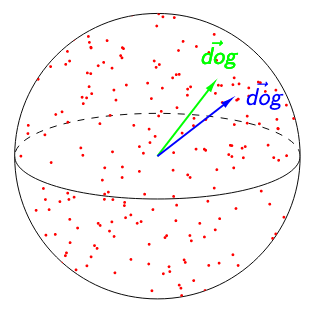
\includegraphics[width=\textwidth]{sources/related_works/imgs/anisotropy_kawin.png}
        \caption{Isotropic distribution}
        \label{fig:iso}
    \end{subfigure}
    \begin{subfigure}[b]{0.3\textwidth}
        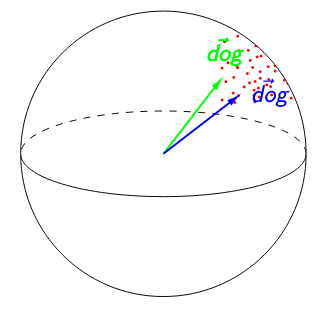
\includegraphics[width=\textwidth]{sources/related_works/imgs/anisotropy_kawin_2.png}
        \caption{Anisotropic distribution}
        \label{fig:aniso}
    \end{subfigure}
    \caption{Schema of anisotropy in a token embedding space. (taken from \citet{ethayarajh-2019-contextual})}
    \label{fig:anisotropy_rw}
\end{figure}


A specific framing of representation degeneration in language modeling has taken the form of \textit{anisotropy}, that is of non-uniformity of the distribution of angular components in language model representations. 

To the best of our knowledge, \citet{ethayarajh-2019-contextual} is the first to describe this phenomenon for contextual representations in natural language. He defines anisotropy as the average cosine similarity between two randomly sampled representations at a given layer. Formally, if $\Upsilon$ outputs representations $\mathbf{h}^i$ are uniformly sampled from the $i$-th layer of a neural network, then the anisotropy level of that layer can be measured as:
\begin{equation}
    \label{eq:anisotropy_cos_def}
    \mathcal{A}_{cos}(\phi_\theta, i) = \frac{1}{\Upsilon^2 - \Upsilon} \sum_{n \neq m} \frac{\langle h^i_n, h^i_m \rangle}{||h^i_n||_2 \cdot||h^i_m||_2 }
\end{equation}

$\mathcal{A}_{cos}(\phi_\theta, i)$ takes a value in $[-1, 1]$, and the distribution of $\mathbf{h}^i$ can be described as anisotropic when $|\mathcal{A}_{cos}|$ takes higher values.

They measure anisotropy on hidden representations obtained across different sentences using this in ELMo \citep{peters-etal-2018-deep}, BERT \citep{devlin-etal-2019-bert} and GPT \citep{Radford2018ImprovingLU}. They find that hidden representations of these models tend to be anisotropic, especially on the deeper layers, and notice that the anisotropy level of GPT takes extreme values (up to $0.97$). In simpler terms, when sampling two output token representations of GPT at random (across documents or not), the cosine similarity between these will be $0.97$ in average. This is unexpected, as a uniform distribution would likely yield orthogonal vectors, especially in high-dimension settings.

\citet{mu2018allbutthetop} explore anisotropy from the perspective of singular value decomposition. They measure an average similarity between each singular vector $u^i \in U^i$ and each hidden representation $h^i$, and by comparing the maximum average similarity (the singular component that is most similar to hidden representations) and the minimum average similarity (the singular component that is least similar to hidden representations). In an isotropic distribution, these similarity levels should be closer as each singular component should almost equally explain all hidden representations. The precise measure is done as such:
$$
\mathcal{A}_{SV}(\phi_\theta, i) = \frac{\min_{u \in U} F(u)}{\max_{u \in U} F(u)}
$$
where $F(u) = \frac{1}{\Upsilon} \sum_{t=1}^{\Upsilon} \exp (\langle u^i, h^i_t\rangle)$.

Here, $\mathcal{A}_{SV}(\phi_\theta, i) \in [0, 1]$ and the distribution is characterized as anisotropic when it is significantly smaller than $1$. They use this measure to show that static embeddings to be anisotropic, and they propose a basic truncation of top singular components to improve their anisotropy. They show that the resulting isotropic static embeddings lead to better performance on downstream tasks.

\citet{Wang2020Improving} take advantage of this spectral viewpoint and use spectrum control to mitigate anisotropy during training. They add a penalization term in the training objective that sets a target for the singular value distribution of the representations. They show that this regularization leads to better performance for language models in monolingual and mutlilingual setups, including for downstream performance.

\citet{rajaee-pilehvar-2021-cluster} use this metric on pretrained language models and come to similar conclusions to \citet{ethayarajh-2019-contextual}. They observe that the spaces spanned by $\mathbf{h}^i$ vectors are split into clusters which may cause anisotropy. They cluster the representations using unsupervised techniques, and compute the clusters barycenters before substracting them from their representations. They show that this post-processing step improves both the STS performance and the results on the NLI benchmarks, while successfully mitigating anisotropy. \citet{rajaee-pilehvar-2022-isotropy} extend the anisotropy diagnosis to the multilingual version of BERT. \citet{haemmerl-etal-2023-exploring} later propose several post-processing techniques to mitigate anisotropy, and show that they improve the performance of sentence embeddings.

\citet{bis-etal-2021-much} prove the existence of a connection between this anisotropy phenomenon and a degeneration similar to the one described in \citet{gao2018representation} (see \Cref{ssec:degeneration}). They show that training language models through cross-entropy optimization leads to a progressive drift of the embeddings towards a common direction, and that such a drift can be measured as an increase in anisotropy levels as a non-centered representation distribution is naturally contained in a narrower region of the space. They remove this common component by substracting the average representation, and show that this simple operation substantially reduces the anisotropy of the distributions according to $\mathcal{A}_{cos}$. Crucially, this connection allows them to formally bridge frequency-related distortions of the embedding space and anisotropy.

Several approaches have taken an opposite stance and have suggested that anisotropy was unharfmul and could even lead to better performance. \citet{ait-saada-nadif-2023-anisotropy} show that anisotropy does not affect clustering performance in sentence representations. \citet{rudman2024stable} propose to add an \textit{isotropy} penalization in the training objective of language models when fine-tuning on downstream tasks, and show slight performance improvements. Finally, \citet{machina-mercer-2024-anisotropy} show that anisotropy does not automatically appear in the output layers of larger language models.


A problem that is closely related to anisotropy is the existence of outlier dimensions in the representations of language models, which are also related with token frequency \citep{puccetti-etal-2022-outlier}. However, outlier dimensions are a form of anisotropy themselves, and most of the mitigation techniques that have been proposed in this subfield are related with quantization issues \citep{ahmadian2023intriguing,nrusimha2024mitigatingimpactoutlierchannels}. Hence, we choose not to include this literature in detail in this section.


\vspace{2em}

The aforementioned works cover diverse topics and aim for different objectives. Nevertheless, they tend to focus on the geometrical interpretability of language models in the representational space. These works show that viewing the activations of these models as vectors that should lie in meaningful spaces can bring performance improvements when leveraged properly. Understanding the geometry of these spaces with respect to data-related properties allows to better understand the behavior of a model, but also to point out limitations that the language modeling paradigm brings, when these spaces are not uniform or when they are too constrained to lead to optimal predictions.





\part[Analysis of the Representations of Language Models]{%
  A good part\\
  %
  \vspace{1cm}
  %
  \begin{minipage}[l]{\textwidth}
    %
    \textnormal{%
      \normalsize
      %
      \begin{singlespace*}
        \onehalfspacing
        %
        You can also use parts in order to partition your great work
        into larger `chunks'. This involves some manual adjustments in
        terms of the layout, though.
      \end{singlespace*}
    }
  \end{minipage}
}

\chapter{On the Scaling Laws of Geographical Representation in Language Models}
\label{chap:geobias}


\subsection{Introduction \& Related work}

In recent years, numerous studies analyzing the hidden representations of self-supervised language models have provided insights into how these models incorporate linguistic knowledge from their training data \citep{gupta-etal-2015-distributional,kohn-2015-whats,shi-etal-2016-string,ijcai2018p796,conneau-etal-2018-cram,jawahar-etal-2019-bert}. 

This line of work has been called probing, as most approaches are generally based on the training of classifiers---or \textit{probes}---upon frozen hidden representations.

Analyzing the representations of language models can point out sociocultural biases that were inherently learned by the models during training \citep{zhao-etal-2018-gender}, and training probes can help with mitigating these biases \citep{ravfogel-etal-2020-null, iskander-etal-2023-shielded}.

Among probing tasks, several works have focused on geographical representations that are implicitly embedded in language models. \citet{lotr} show that coordinates of places in the Middle-Earth can be predicted by just using the co-occurence matrix extracted from the Lord of the Rings novels. \citet{faisal-anastasopoulos-2022-geographic} build networks from geographical representations based on monolingual and multilingual models of different sizes. They show that all models embed more accurate geographical representations for countries of the Global North.

This geographical discrepancy can be explained by biases that are inherent to the datasets used for pretraining \citet{faisal-etal-2022-dataset}. Imbalanced frequency distributions of geographical references in pretraining data causes distortions in the representational space \citep{zhou2021freqbased}. These distortions lead to a loss in the models' ability to differentiate between under-represented locations.

Recently, \citet{gurnee2023language} have probed large language models from the Llama-2 suite \citep{touvron2023llama} to extract coordinates of prompted locations from hidden representations across layers. They show that models ranging from 7B to 70B parameters are able to convincingly embed geographical coordinates on a world map when representing basic prompts.

In this work, we propose to extend the analysis by \citet{gurnee2023language} to smaller language models, in order to observe how scale affects the ability of models to implicitly embed geographical information from raw training data. We show that such ability consistently improves with model size, and that even tiny models are able to produce visually meaningful world maps.

We make several contributions:
\begin{itemize}
    \item We show that geographical information can be extracted to a certain extent from representations at every model scale;
    \item We observe that larger models are more geographically biased than their smaller counterparts;
    \item We find that the performance of models in terms of geographical probing is correlated with the frequency of corresponding country names in the training data.
\end{itemize} 

\subsection{Scaling Laws of Geographical Probing}
\label{sec:scaling}
\begin{figure*}[h]
    \centering
    \begin{subfigure}[b]{0.43\textwidth}
         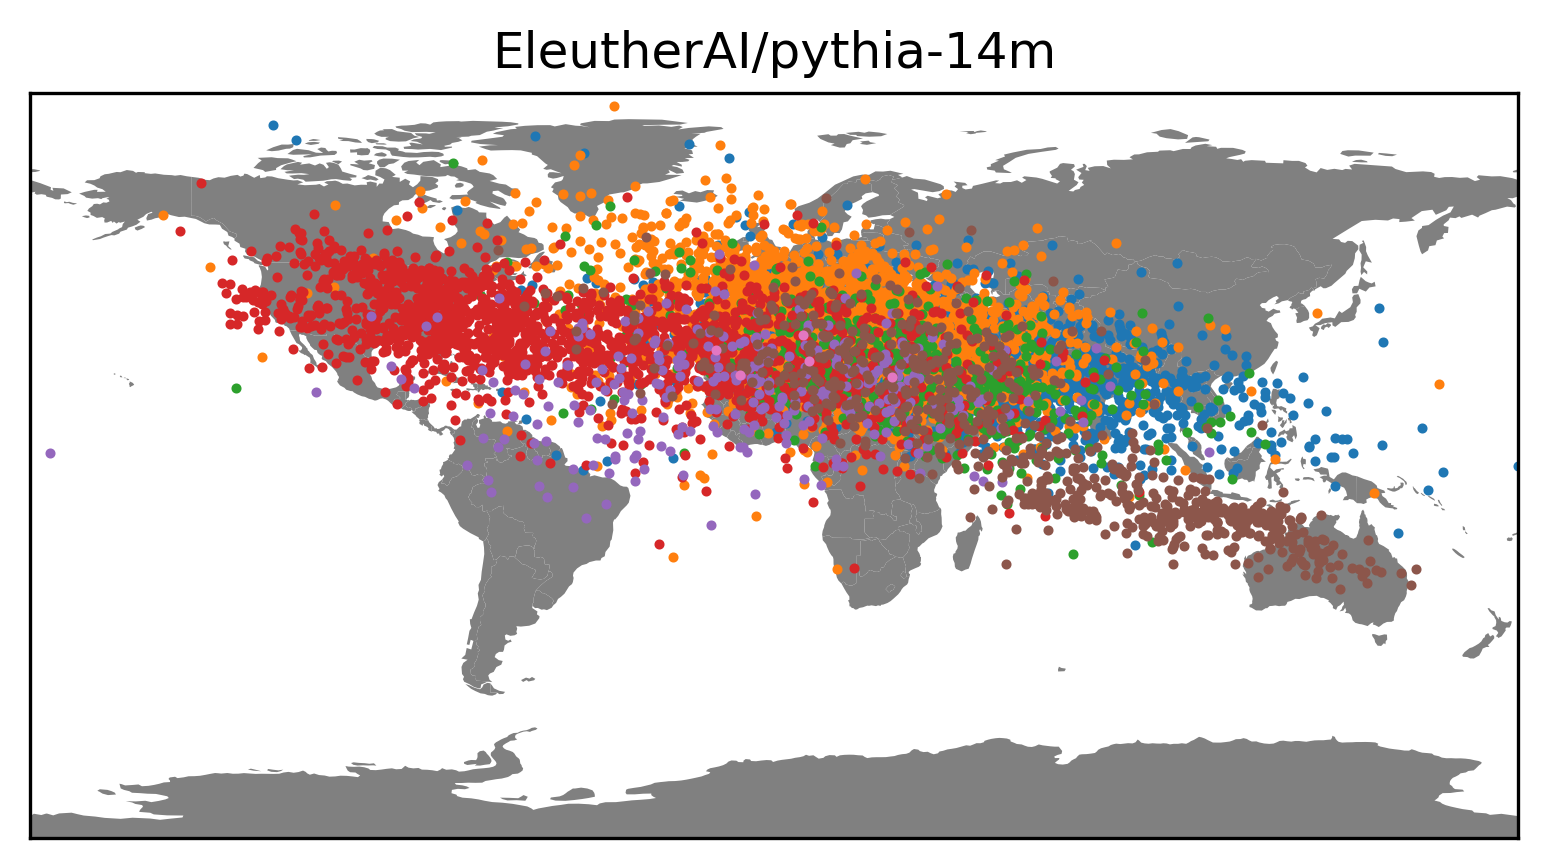
\includegraphics[trim={0 0 0 0.7cm},clip,width=\linewidth]{sources/part_1/geographical/imgs/pythia-14m.png}
         \caption{Pythia 14M ($R^2 = 34.34$)}
         \label{fig:14m_map}
         \vspace{1em}
    \end{subfigure}
    \begin{subfigure}[b]{0.43\textwidth}
         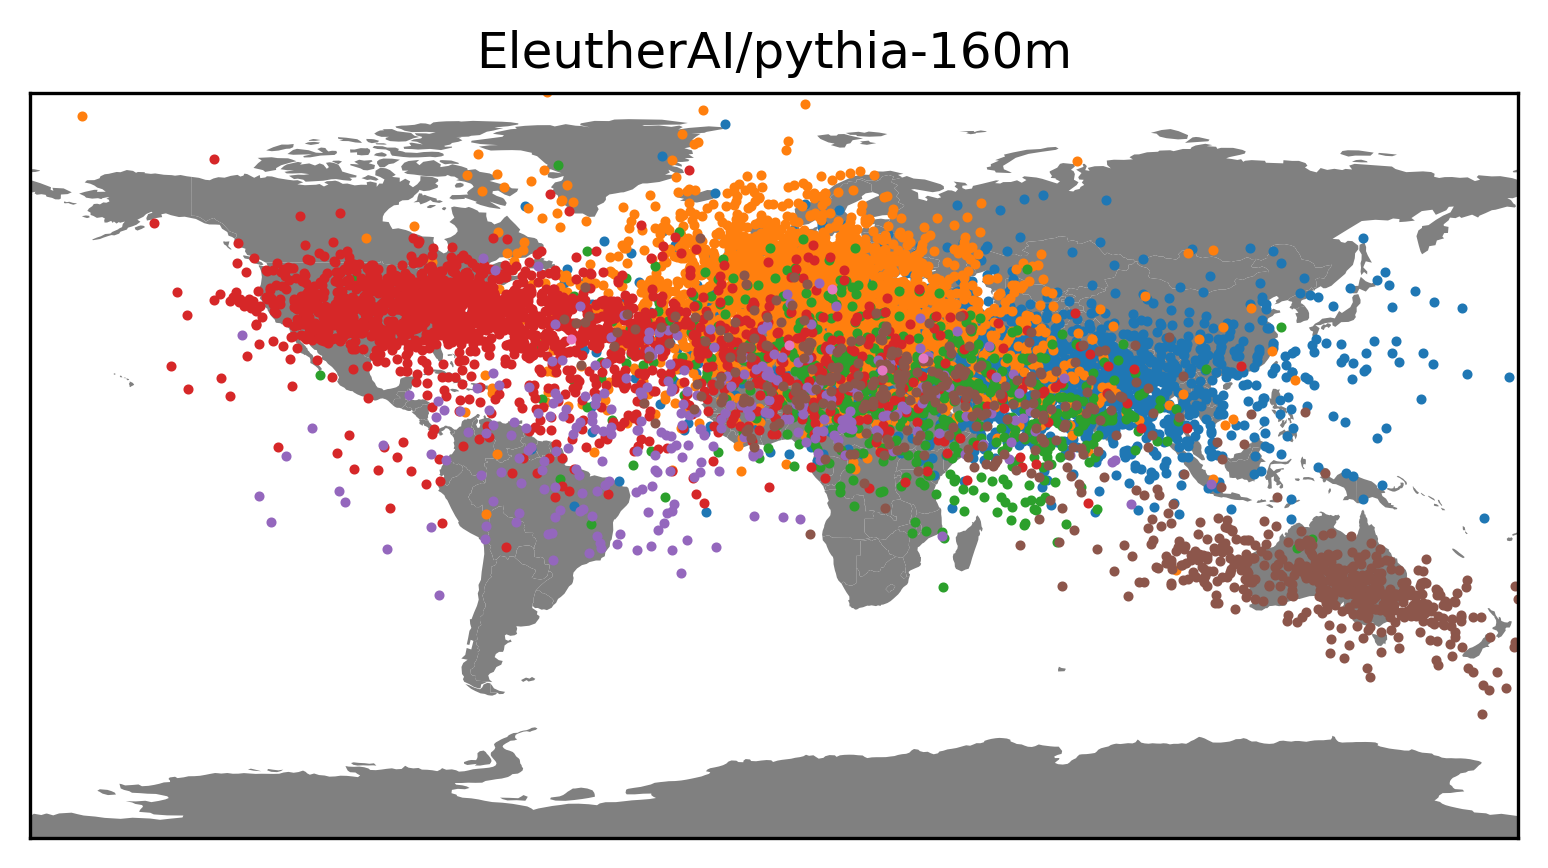
\includegraphics[trim={0 0 0 0.7cm},clip,width=\linewidth]{sources/part_1/geographical/imgs/pythia-160m.png}
         \caption{Pythia 160M ($R^2 = 55.28$)}
         \label{fig:160m_map}
        \vspace{1em}
    \end{subfigure}
    \begin{subfigure}[b]{0.43\textwidth}
         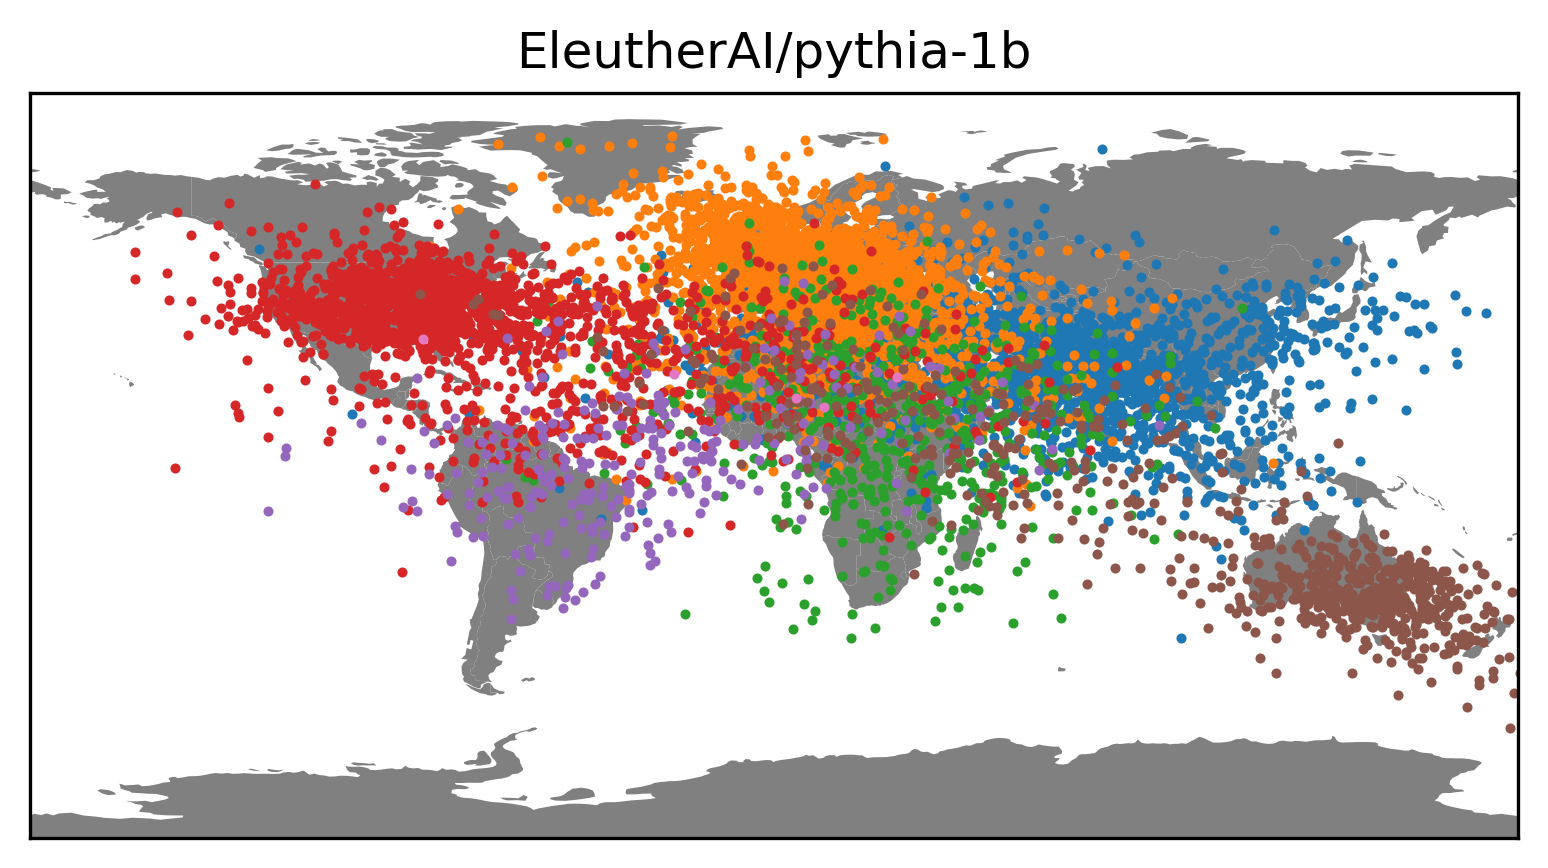
\includegraphics[trim={0 0 0 0.7cm},clip,width=\linewidth]{sources/part_1/geographical/imgs/pythia-1b.png}
         \caption{Pythia 1B ($R^2 = 67.94$)}
         \label{fig:1b_map}
    \end{subfigure}
    \begin{subfigure}[b]{0.43\textwidth}
         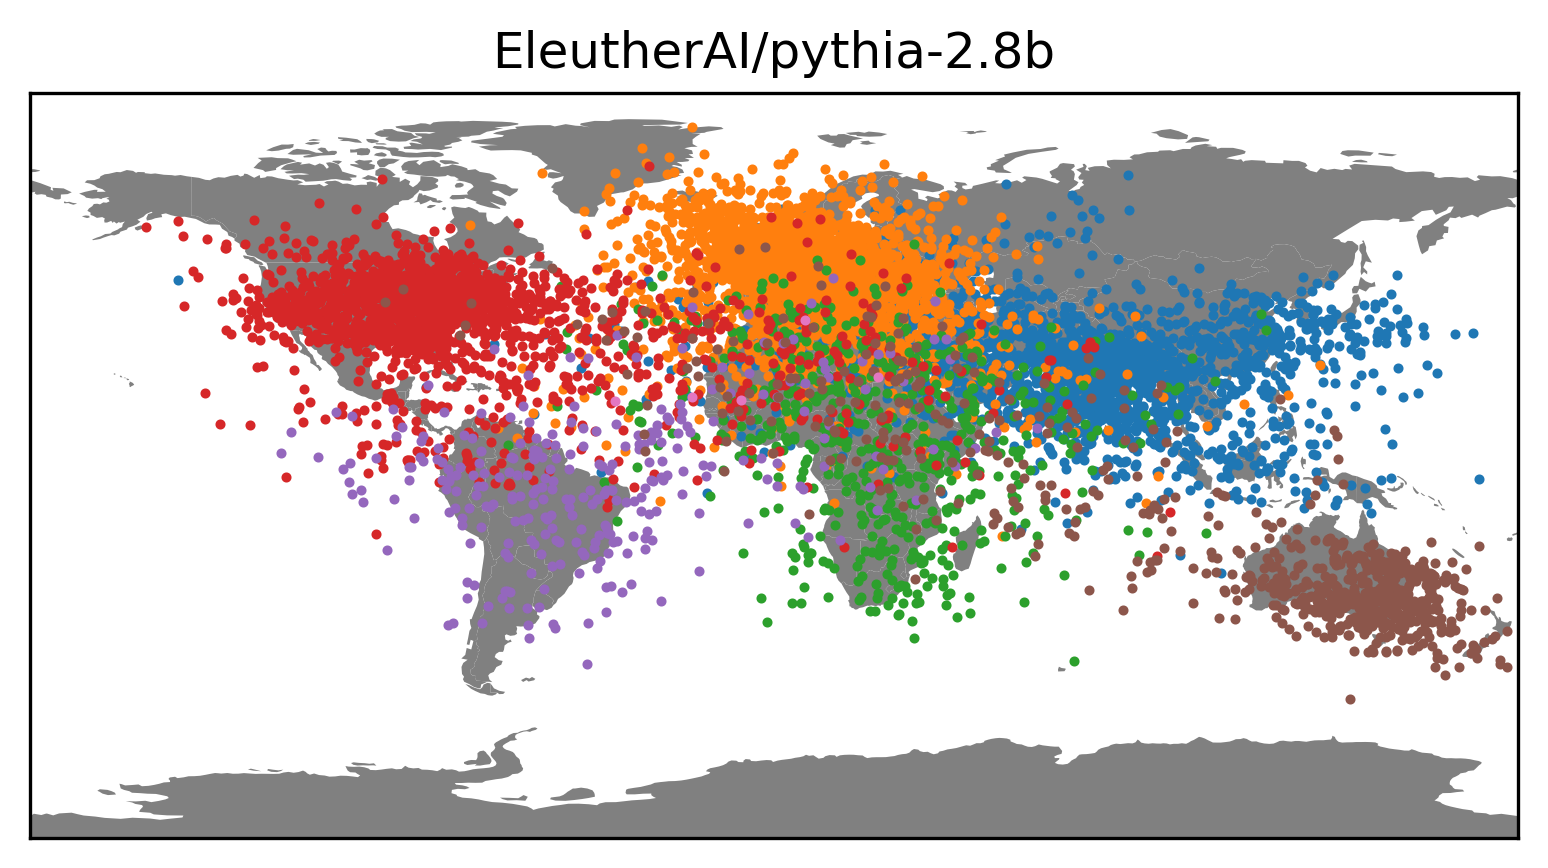
\includegraphics[trim={0 0 0 0.7cm},clip,width=\linewidth]{sources/part_1/geographical/imgs/pythia-2.8b.png}
         \caption{Pythia 2.8B ($R^2 = 74.97$)}
         \label{fig:2.8b_map}
    \end{subfigure}
    \caption{Predicted coordinates of test set instances for different model sizes. Each color represents a different continent.}
    \label{fig:maps}
\end{figure*}

In this section, we train geographical probes for a wide variety of models at different scales.

\subsubsection{Methodology}

We use the World dataset from \citet{gurnee2023language} as a geographical data source. It contains 39,504 location names from the whole world along with corresponding longitude and latitude. We use the same train-test split strategy as in the original article, thus keeping 20\% of samples for testing purposes.

For each location name $X$, we prompt models with the text: ``\textit{Where is $X$ in the world?}''. We then infer with a given model on the whole dataset, and use the last token belonging to the entity $X$ as the model's representation. To follow the linear probing paradigm used in \citet{gurnee2023language}, we train a Ridge linear regressor \citep{ridge} to predict latitude and longitude based on the model's representations. We then measure the probe's performance on the test set using the $R^2$ correlation coefficient.

\subsubsection{Results}
In \autoref{fig:maps}, we display the predictions of the probe for the most performant layer, which is generally the last one. We observe that geographical information can be extracted from models even for a very small parameter count. The performance of the probes seem to increase with the model size.

\begin{figure}[h]
    \centering
    \begin{subfigure}[b]{0.37\textwidth}
         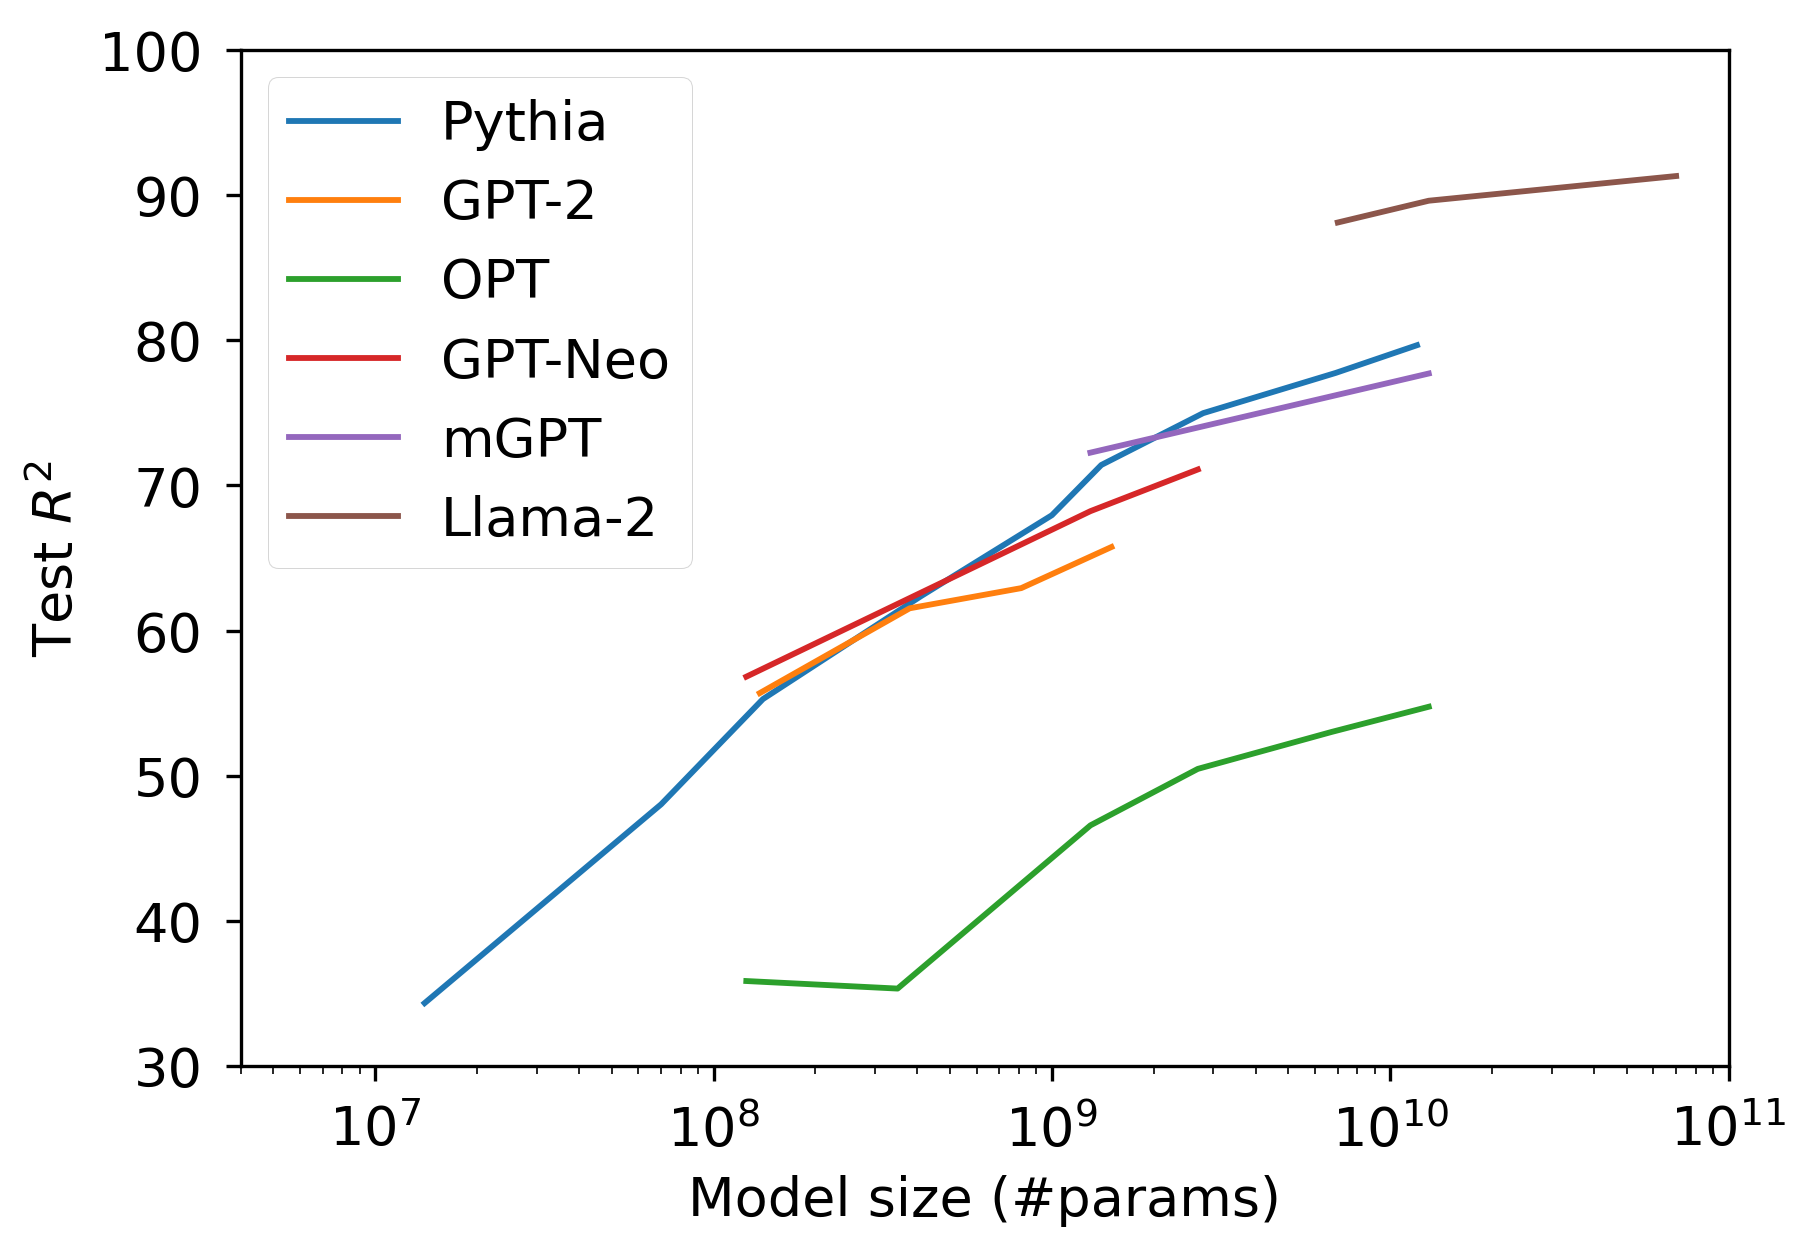
\includegraphics[width=\linewidth]{sources/part_1/geographical/imgs/r_square_world_decoders.png}
         \caption{Decoder models}
         \label{fig:decoder_evol}
         \vspace{1em}
    \end{subfigure}
    \begin{subfigure}[b]{0.37\textwidth}
         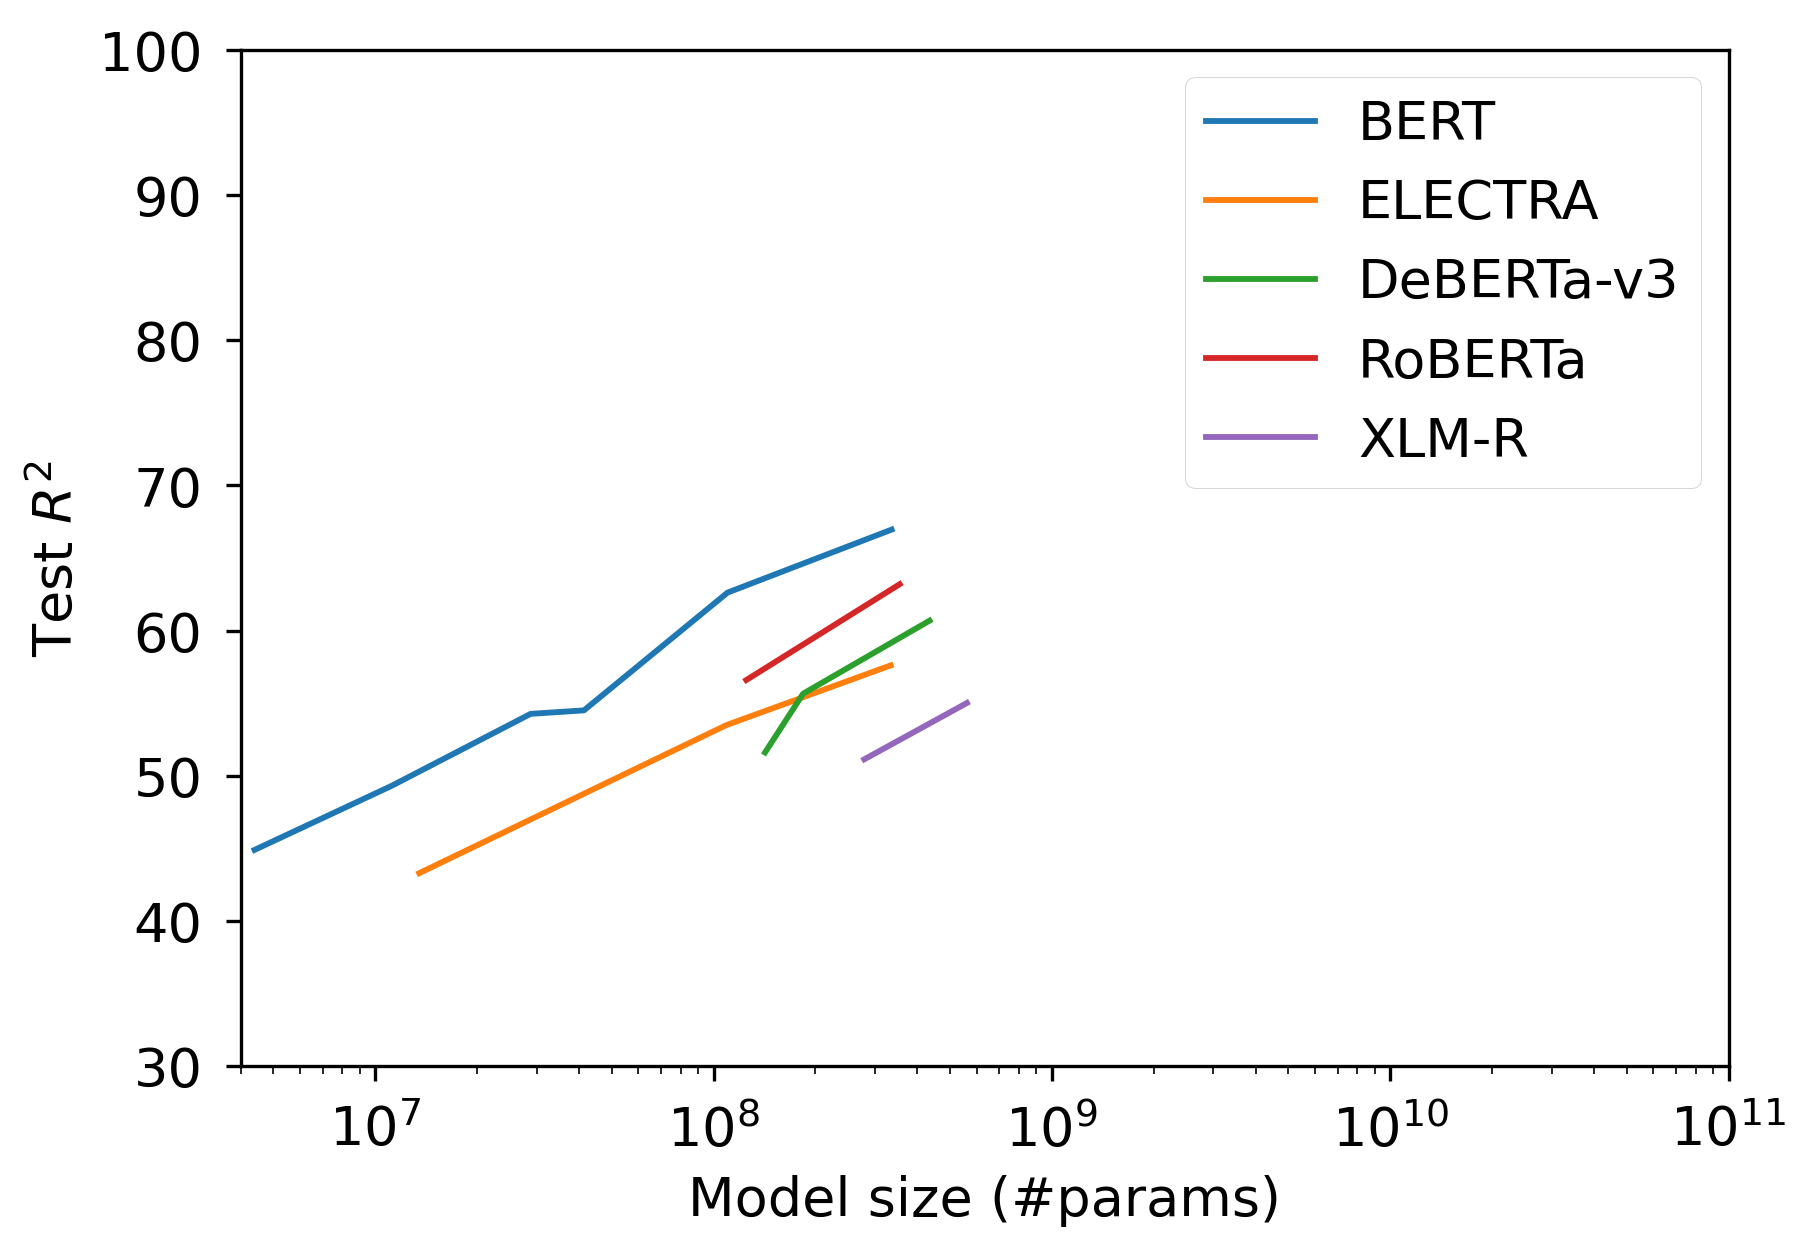
\includegraphics[width=\linewidth]{sources/part_1/geographical/imgs/r_square_world_encoders.png}
         \caption{Encoder models}
         \label{fig:encoder_evol}
    \end{subfigure}
    \caption{Evolution of the $R^2$ coefficient on the test set for various model suites.}
    \label{fig:evol}
\end{figure}

We show in \autoref{fig:evol} that the performance of language models evolves consistently with model size, regardless of the architecture. We validate this property on several decoder model families: GPT-2 \citep{gpt2}, OPT \citep{zhang2022opt}, Pythia \citep{pythia}, GPT-Neo \citep{gpt-neo}, the multilingual mGPT \citep{shliazhko2023mgpt}, and Llama-2 \citep{touvron2023llama}. We also display results for several encoder models: BERT \citep{devlin-etal-2019-bert,turc2020wellread}, RoBERTa \citep{roberta}, ELECTRA \citep{electra}, and DeBERTa-v3 \citep{deberta}. This property also applies for encoder models, for which we notice that the BERT suite unexpectedly outperforms its counterparts. The performance of encoder models is comparable with the one of equivalent decoder models. We can underline the fact that BERT-Large (336M parameters) is as accurate as the three times larger Pythia-1B.

Interestingly, the multilingual XLM-R \citep{conneau2020unsupervised} underperforms its counterparts, even though multilingual data must have increased the training data's geographical diversity to some extent \citep{faisal-anastasopoulos-2021-investigating}. The mGPT suite also slightly underperforms Pythia models at equivalent model sizes.

We verified that the better performance of larger models was not solely related with the ability of the probes to extract better patterns from their higher-dimensionality hidden representations. We achieved this by concatenating representations with themselves to increase dimensionality without introducing novel knowledge. It led to slightly worse performance for all tested models, thus showing that performance was not a consequence of dimensionality alone.

\subsection{Geographical Bias and Scale}

In \autoref{fig:maps}, it seems at first glance that as the model size increases, the predictions tend to be more accurate for locations of the Southern Hemisphere. In this section, we propose to quantify this hypothesized behavior by measuring the bias across countries and continents for various scales. We also correlate the models' accuracy with both lexical and geographical factors.

\subsubsection{Measuring bias}

We group probe performance as measured by mean-squared error (MSE) on predicted coordinates, and average measures by continent in \autoref{fig:continent_perf}. While we notice that the performance increases consistently for every continent, we do not observe a significant reduction in the performance gap across continents as model size increases.

\begin{figure}
    \centering
    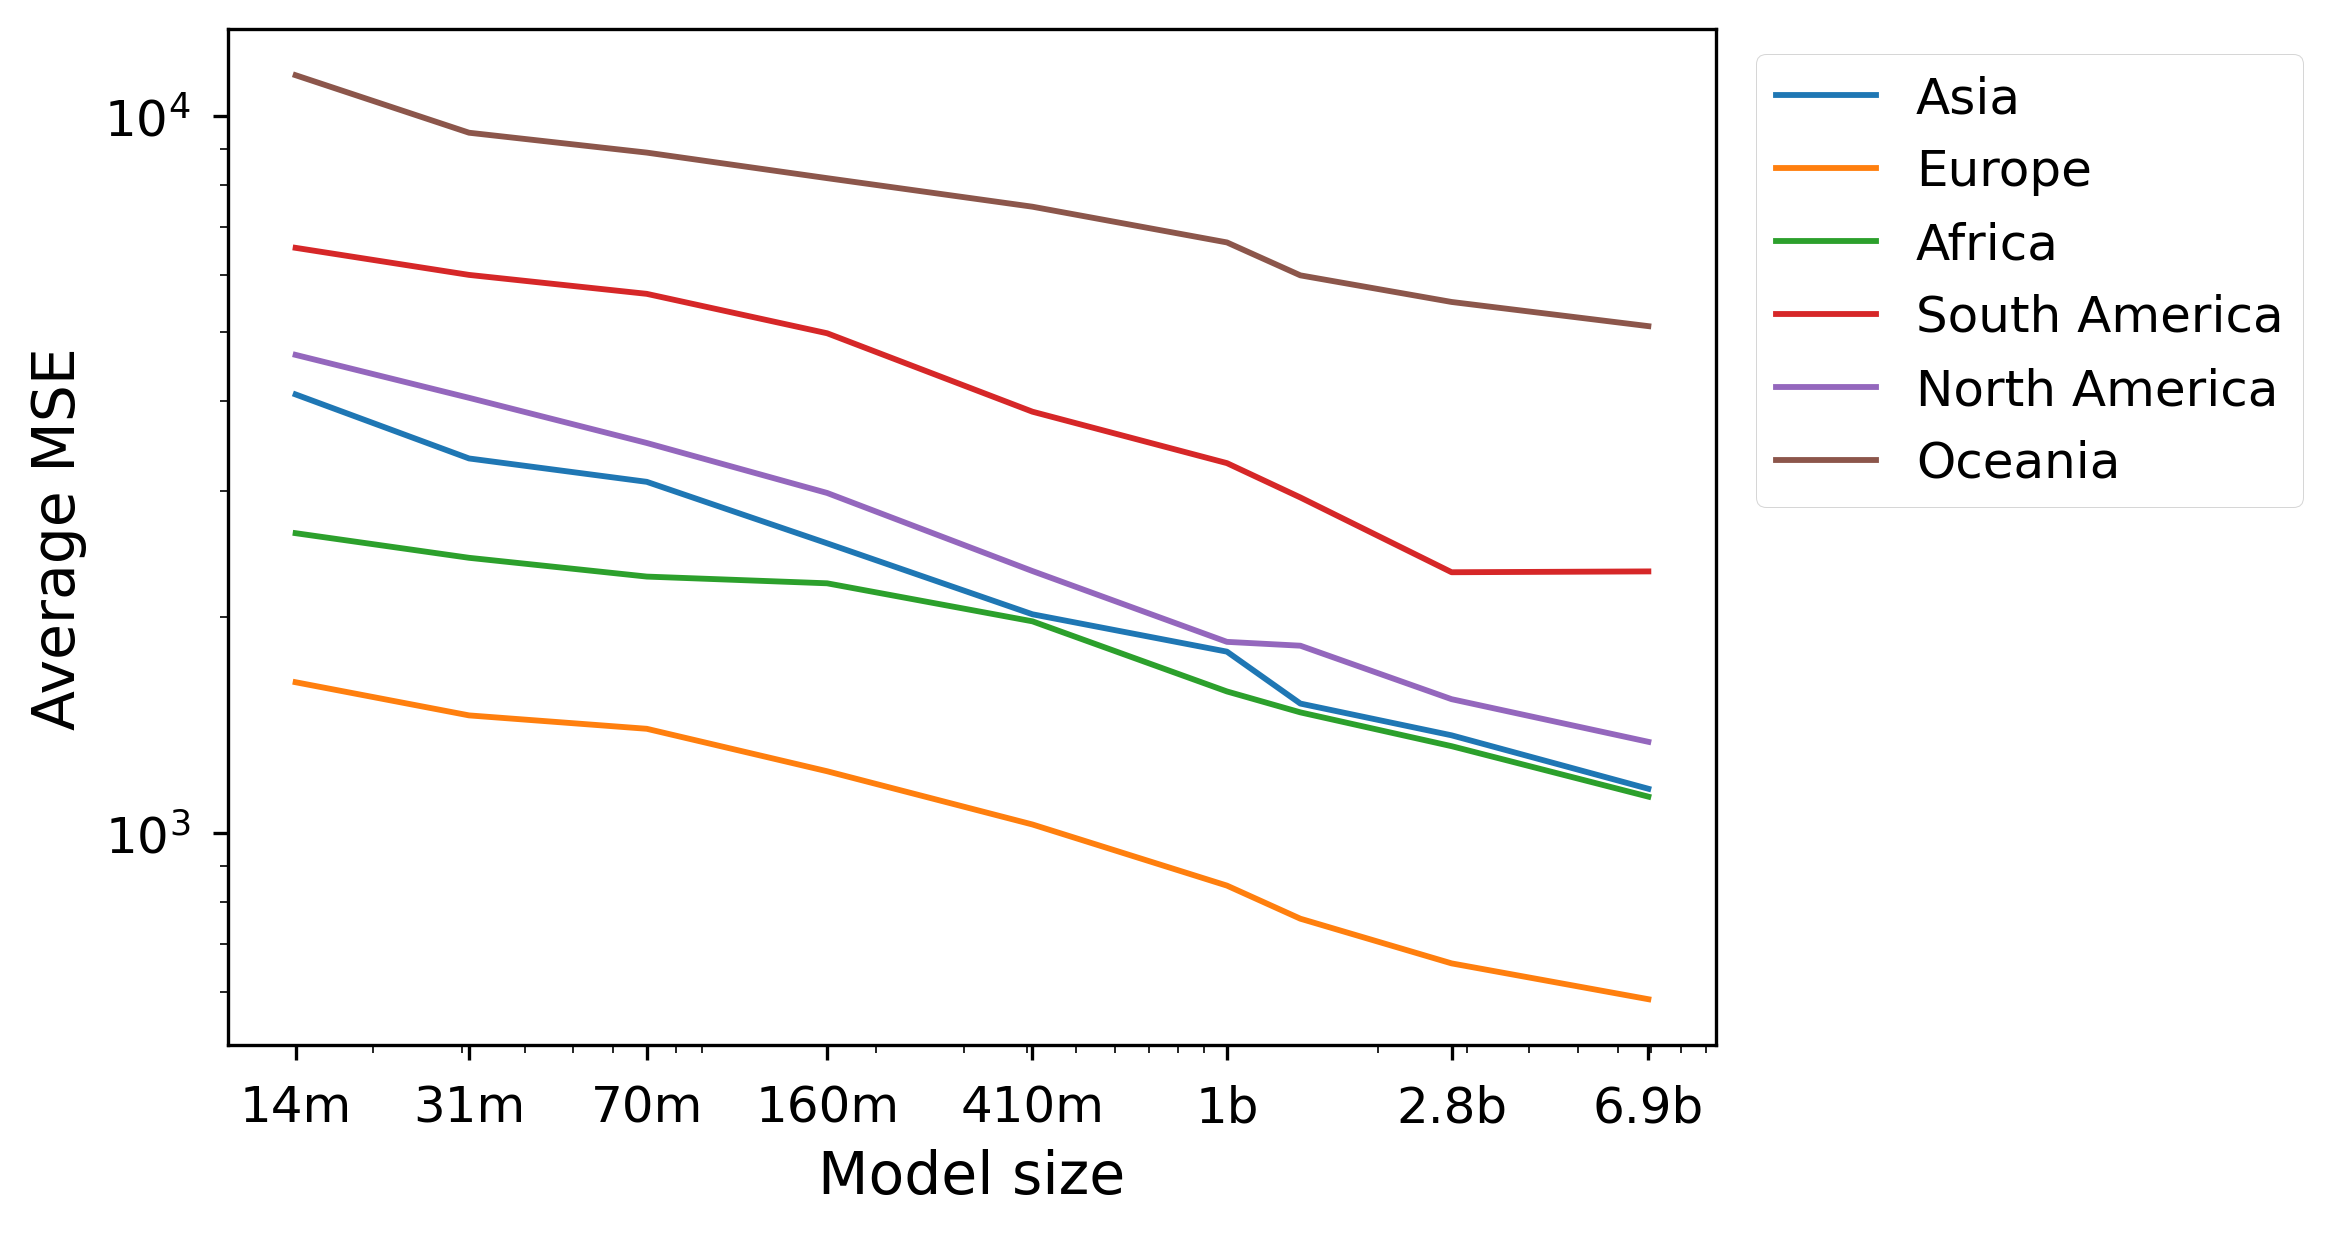
\includegraphics[width=0.9\linewidth]{sources/part_1/geographical/imgs/mse_continent.png}
    \caption{Average MSE by continent for different sizes in the Pythia suite.}
    \label{fig:continent_perf}
\end{figure}

To measure the heterogeneity of the probing performance of language models across countries, we use the Gini coefficient \citep{gini1912variabilita} that is widely used in economics. Given a series of observed variables $(x_i)_{i\in[1, N]}$, the Gini coefficient is defined as:
$$
Gini(x) = \frac{\sum_{i,j \in [1, N]} |x_i - x_j|}{N \cdot \sum_{i = 1}^{N} x_i}
$$

A Gini coefficient of 1 reflects perfect heterogeneity, while a Gini of 0 implies perfect homogeneity.

\begin{figure}
    \centering
    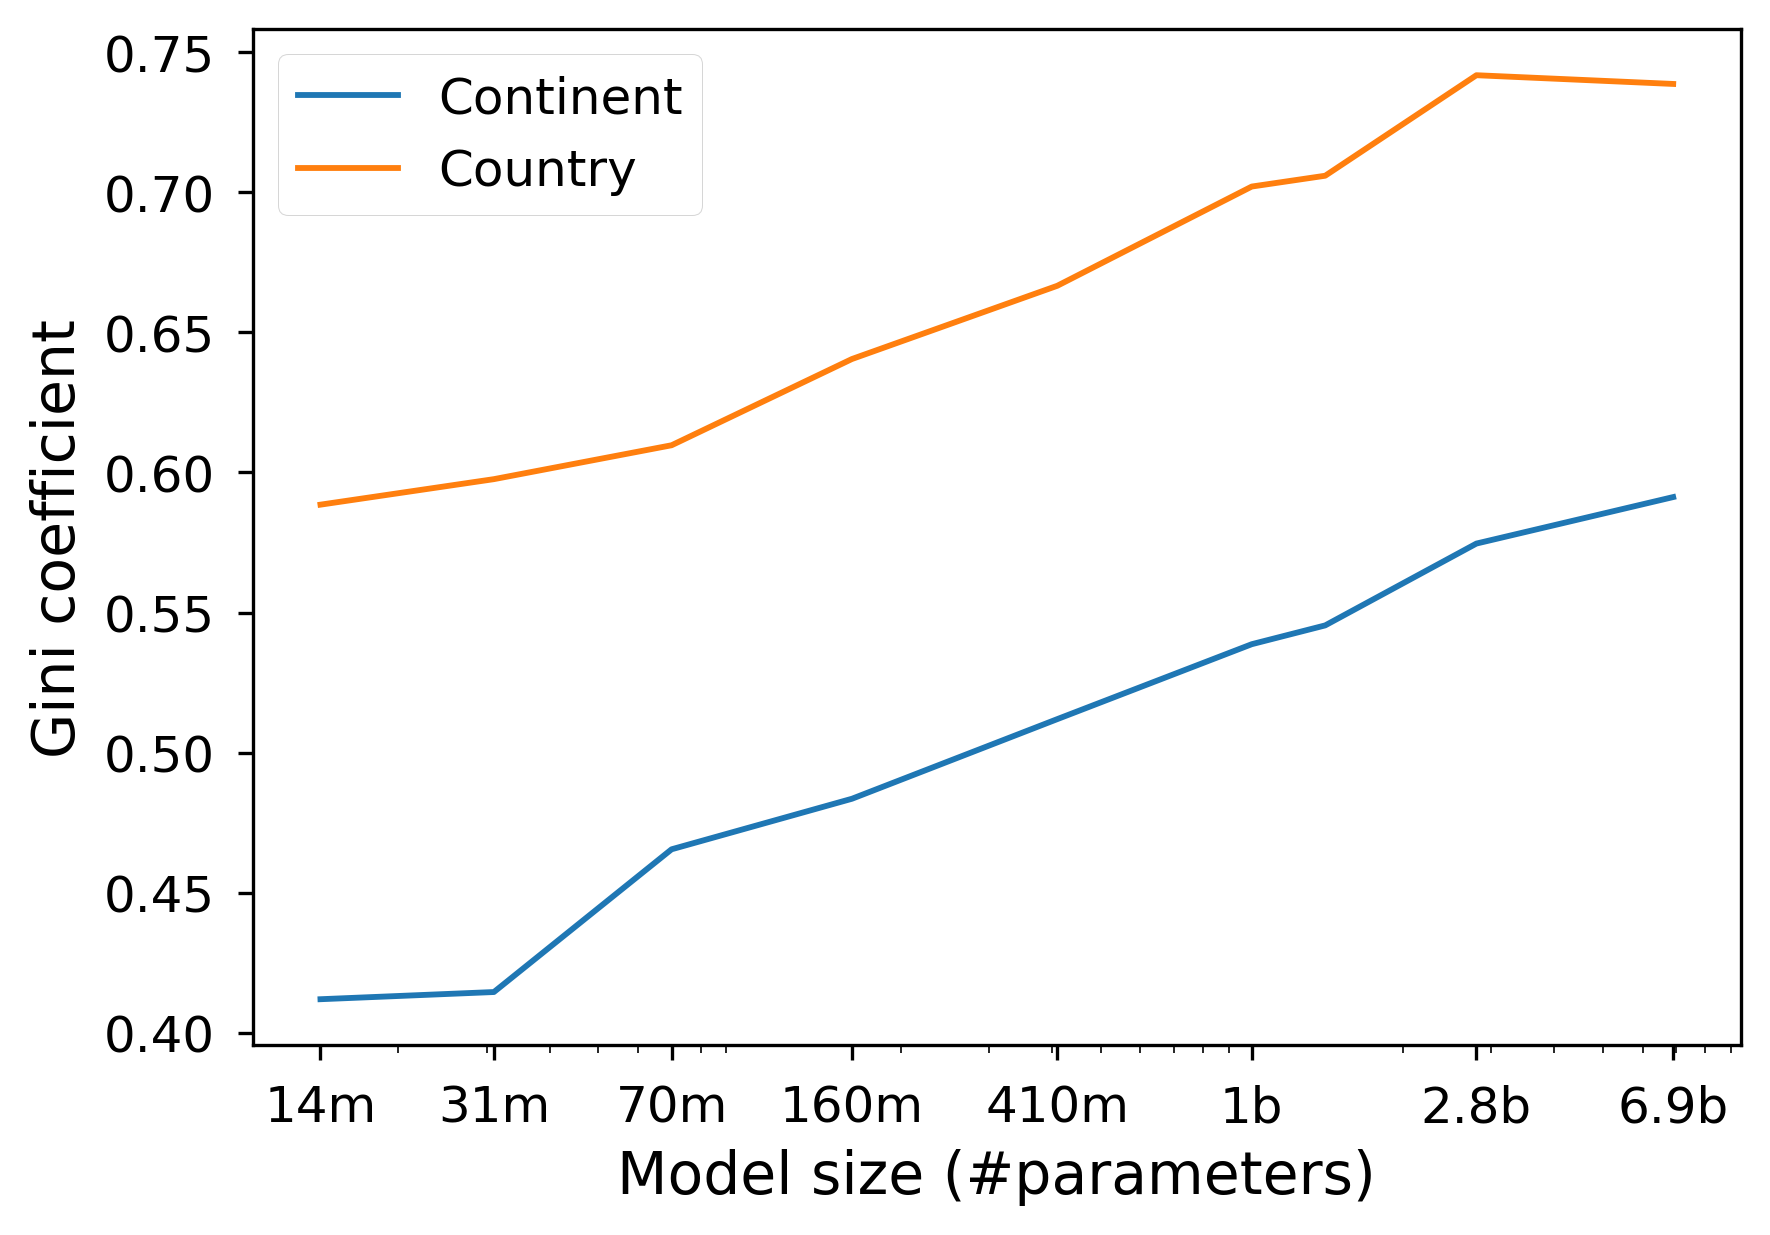
\includegraphics[width=0.75\linewidth]{sources/part_1/geographical/imgs/gini_combined.png}
    \caption{Gini coefficients of MSE on the test set averaged by country or by continent, as model size increases.}
    \label{fig:ginis}
\end{figure}

\autoref{fig:ginis} shows that the larger the model is, the more heterogeneous the probe performance is across countries and continents. This contradicts the impression given by \autoref{fig:maps}, and shows that scale does not solve the geographical discrepancy caused by bias inherent to the training data.

\begin{figure}
    \centering
    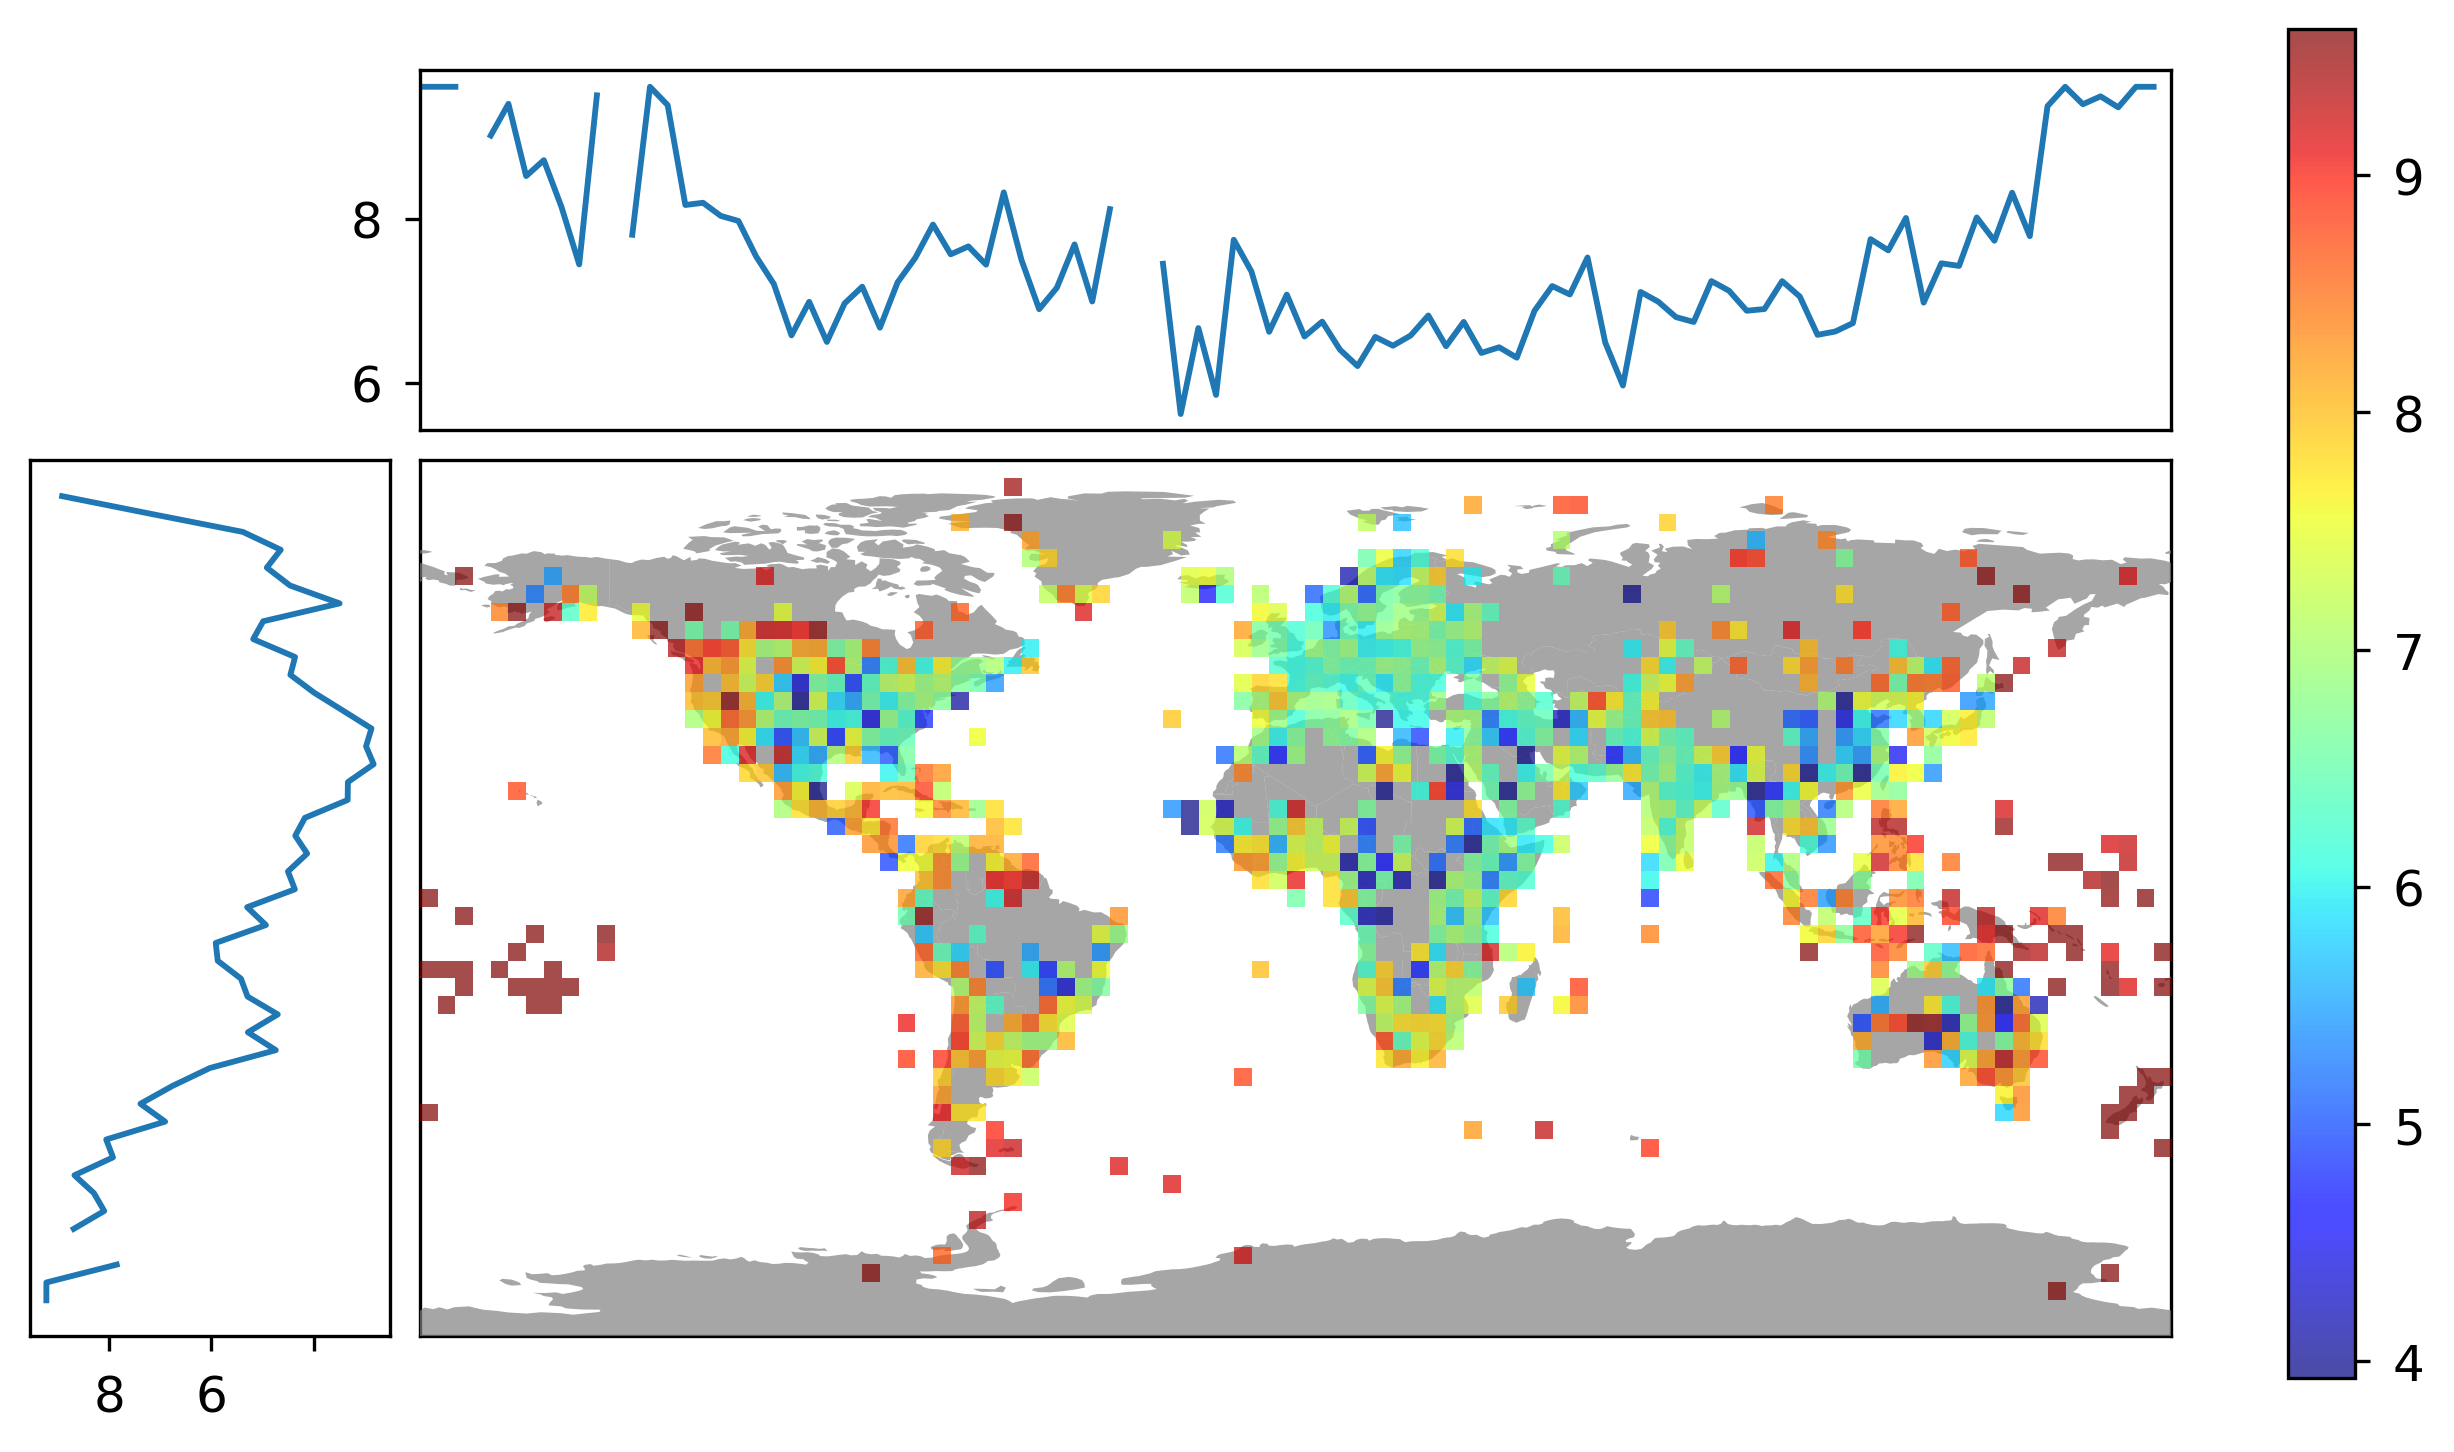
\includegraphics[width=0.9\linewidth]{sources/part_1/geographical/imgs/heatmap_100_50.png}
    \caption{Test log-MSE for Pythia-1B as plotted on a World map.}
    \label{fig:heatmap}
\end{figure}

In \autoref{fig:heatmap}, we locally average log-MSE on a World map, and report results agglomerated according to latitude and longitude. We clearly observe that the model performs poorly in Oceania, South Asia and South America. We also see that the error is minimal around the latitude of North America and Europe, while it increases in the Southern Hemisphere.

\subsubsection{Identifying sources of bias}
We attempt to correlate the performance of our geographical probes with several factors. First, the dataset from \citep{gurnee2023language} provides each location with an estimate of the corresponding population count when relevant. We also consider training data distribution as a potential factor of heterogeneity. Finally, we consider latitude and longitude as potential factors of bias.


To account for training data distribution, we look for exact string matches of country names from the \citet{gurnee2023language} dataset in an extract of The Pile \citep{gao2020pile} containing 3.5 million samples \footnote{\url{https://huggingface.co/datasets/ola13/small-the\_pile}}. We select this dataset as it was used to pretrain the models from the Pythia suite \citep{pythia} we evaluate in this section. We find 15 million matches, covering 98\% of the countries of the dataset.

We do not count occurrences of location names directly, as matching locations on the basis of their names does not account for named entity ambiguity. An example of ambiguous location name is \textit{Fully}, which is a town in Switzerland. An exact match strategy overestimates by large margins the occurrence count of this location, because of the corresponding English word \textit{fully}. Disambiguation techniques have been designed \citep{hoffart-etal-2011-robust, orr2020bootleg}, but we prefer to avoid the risk of bias propagation and the cost of using such methods on a large corpus.

\begin{figure}
    \centering
    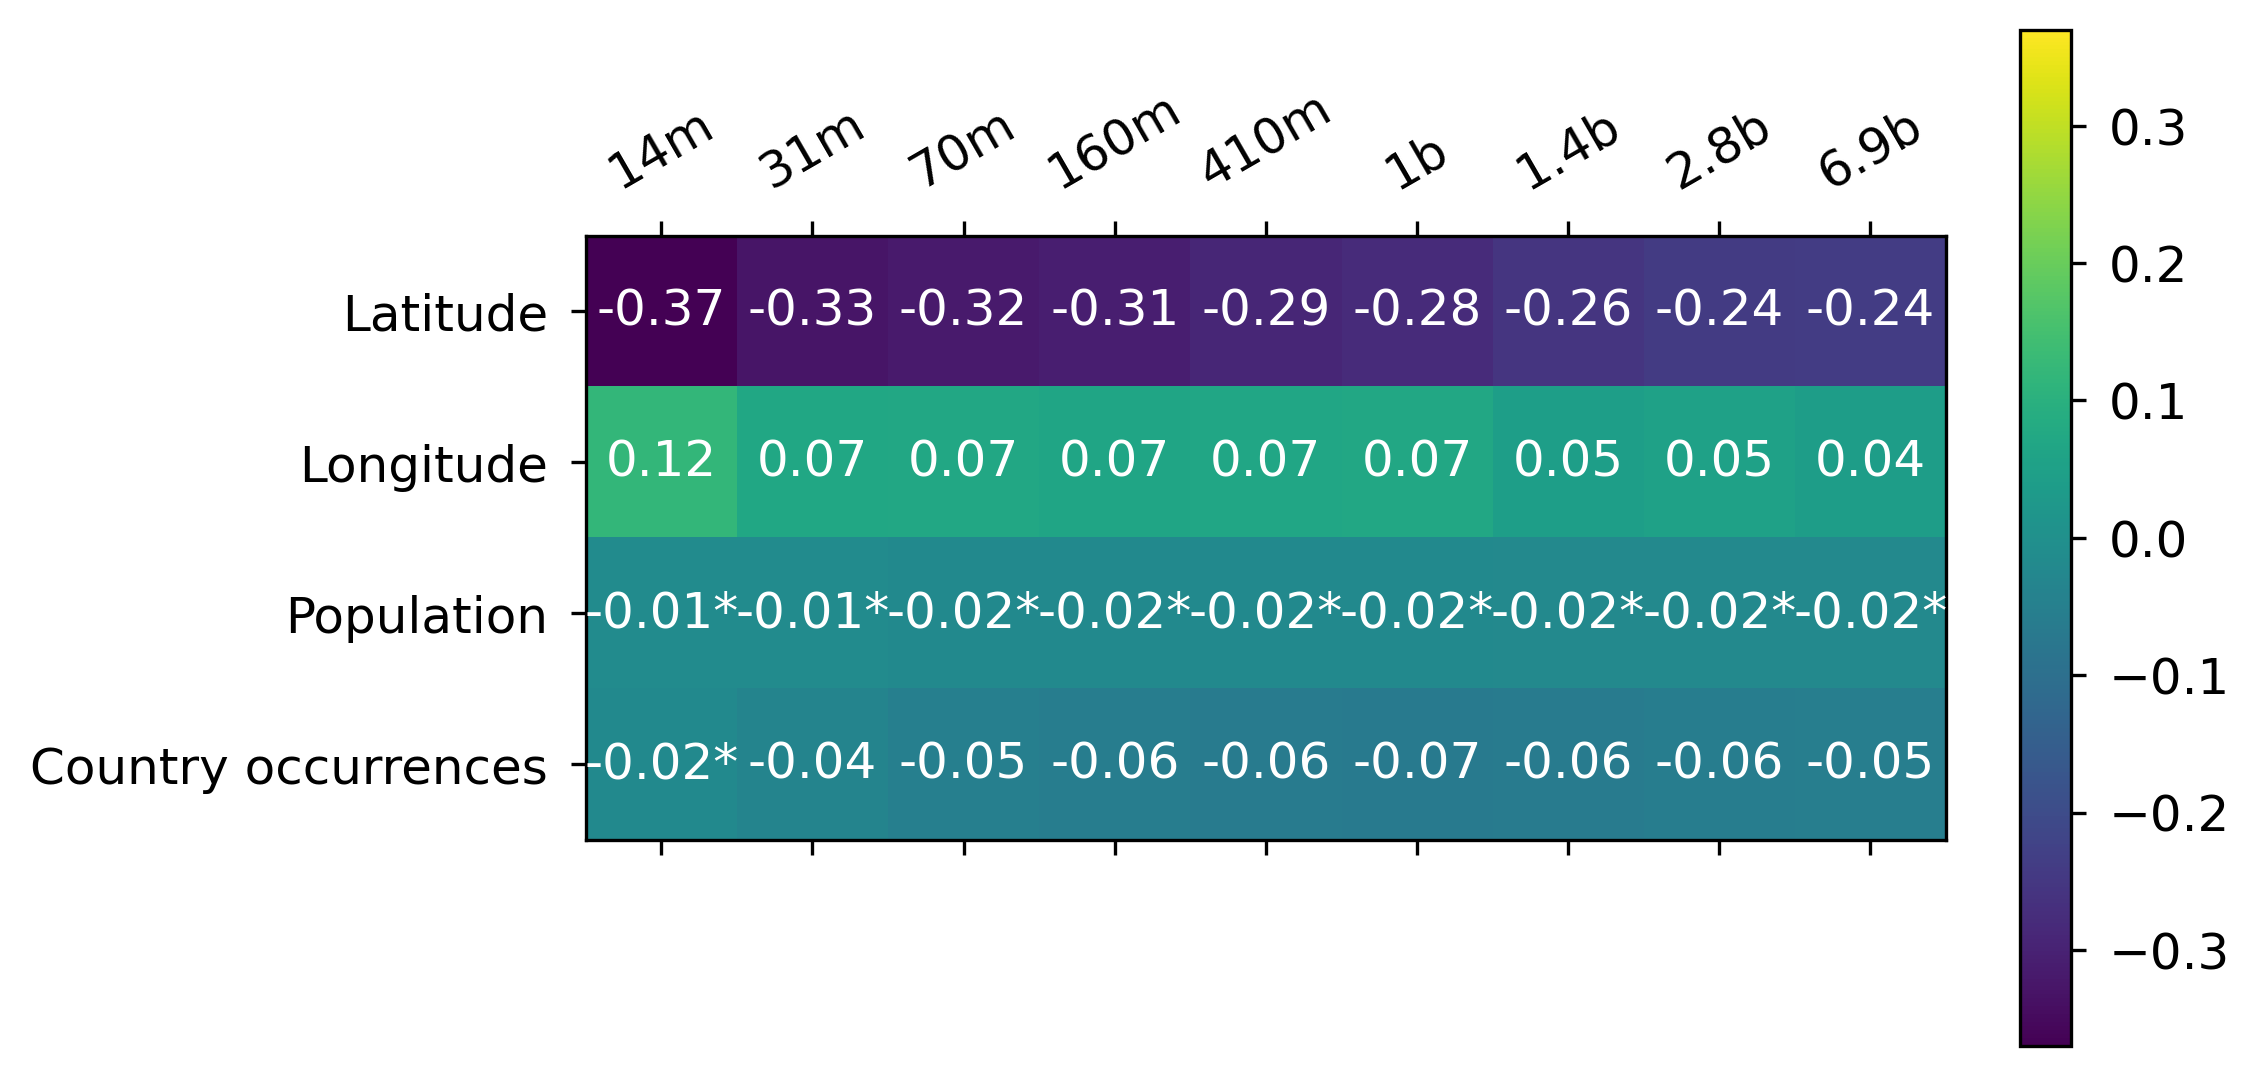
\includegraphics[width=0.9\linewidth]{sources/part_1/geographical/imgs/correl_size.png}
    \caption{Pearson correlation coefficients of various factors with location-wise MSE, for several Pythia model sizes. *: Tests that yielded p-values above 0.05.}
    \label{fig:correl}
\end{figure}

We display Pearson correlations between each of the aforementioned factors and the entity-level MSE for each model size in \autoref{fig:correl}. As in \autoref{fig:14m_map}, we observe that the error on coordinates prediction is negatively correlated with the latitude, i.e. southern locations are less accurately identified. This correlation slowly decays as the model size increases. Meanwhile, longitude seems to be mildly correlated with the probe performance.

Interestingly, the population count is not correlated with the error level. The occurrence count of the location country is negatively correlated with the error level, thus showing that the more country names appear in the training dataset, the more the probes are able to recover coordinates from locations in these countries. However, this correlation is mild and even below the significance threshold for the smallest model.

We also measure the correlation between country occurrences and other metrics to account for the bias inherent to the data. We observe that country name occurrences are positively correlated with latitude with a p-value of 0.06, and not correlated with the longitude. More importantly, the population count of a country and the count of this country name in the data are heavily correlated (factor of +0.52 and p-value of 3e-23). Thus, even though the data seems guided by demographic factors, this is not the case of the model's representations.

\subsection{Discussion}
\label{sec:discussion}
We believe that quantifying sociocultural bias in representations of language models and pretraining datasets allows to better understand the roots of the biases that can be observed during generation.

\citet{parrots_bender} discuss the relevance of scaling models to ever larger magnitudes, with regard to environmental and financial costs. Our study shows that scale can also increase language modeling bias when it comes to geographical representation, given a pretraining dataset. We advocate in favor of measuring and mitigating bias in pretraining datasets to avoid scaling bias along with performance.

\subsection*{Conclusion}
In this study, we show that a wide variety of language models, varying in architecture and sizes, implicitly embed geographical data to some extent. As we consider larger models, the performance of geographical probes consistently increases towards levels shown in \citet{gurnee2023language}.

We show numerically that the geographical probe performance is correlated with latitude across model sizes, but also with the number of occurrence of corresponding country names in the pretraining data. Conversely, the population count of the location seems uncorrelated with the probe performance. This indicates that a minority of people benefit from better geographical understanding when using language models, which does not maximize the social utility of these systems.

While it may initially seem that this performance increase mitigates heterogeneity between Southern and Northern countries, we actually show that larger models tend to be more biased according to the Gini coefficient taken on prediction error. This tends to show that scaling language models can amplify discrepancies in their geographical knowledge.




% \section*{Acknowledgements}
% This work was funded by the last authors' chair in the PRAIRIE institute, funded by the French national agency ANR as part of the ``Investissements d'avenir'' program under the reference ANR-19-P3IA-0001.
% We thank Stella Biderman for her insightful advice.

% % We would like to thank Roman Castagné for useful discussions that led to focusing on observing the effect of anisotropy in the self-attention process.

% % Entries for the entire Anthology, followed by custom entries
% \section*{Bibliographical References}
% \label{sec:reference}
% \bibliography{sources/part_1/geographical/lrec-coling2024-natbib}
% \bibliographystyle{sources/part_1/geographical/lrec-coling2024-natbib}

% \section*{Language Resource References}
% \label{lr:ref}
% \bibliographylanguageresource{sources/part_1/geographical/lrec-coling2024-natbib}
% \bibliographystylelanguageresource{sources/part_1/geographical/lrec-coling2024-natbib}

% \clearpage

% \appendix


%%% Local Variables:
%%% mode: latex
%%% TeX-master: t
%%% End:


\chapter{Studying Language Model Saturation via the Softmax Bottleneck}
\label{chap:softmax_bottleneck}
In \Cref{chap:geobias}, we explored the knowledge bias phenomenon as the size of the models increases. \citet{zhou2021freqbased} describe the connection between knowledge bias and frequency-based distortions such as anisotropy (see \Cref{sec:rw_degeneration}). In this chapter, we explore these geometrical distortions for various model sizes, with a particular focus on training dynamics.

In \Cref{sec:rw_degeneration}, we discussed the representation degeneration phenomenon from the various perspectives offered by the literature. However, the observations made in the aforementioned works were mostly made on relatively small-scale models of dimensions comparable to BERT \citep{devlin-etal-2019-bert} or models from the GPT-2 suite \citep{gpt2}.

We recall that language models are usually composed of a neural network $f_\theta$ that takes sequences of tokens $(\mathbf{w}_{<t}) \in [1,V]^{t-1}$ as inputs and produces a relatively low-dimensional contextual representation in $\mathbb{R}^{d_m}$, where $d_m$ is the \textit{hidden dimension} of the model. They then rely on a \textit{language modeling head} that produces logits for contextual token probabilities. A common choice for the language modeling head is a linear layer with parameter $W \in \mathbb{R}^{V \times d_m}$, where $V$ is the vocabulary size. The resulting next-token probability distribution is then given by:
$$
p(w_t) = \phi_\theta(\mathbf{w}_{<t}) = \sigma (W f_\theta(\mathbf{w}_{<t}))
$$
where $\sigma$ is the softmax function.

As discussed in \Cref{ssec:scaling_law}, the current trend consists in scaling up the generative pretraining approach introduced with GPT-2, which implies training neural models made of several billions of parameters on gigantic web-mined text corpora \citep{brown2020language, touvron2023llama, almazrouei2023falcon, jiang2023mistral}. However, training and serving such highly parameterized models raises energy and hardware-related problematics, which motivates for looking into achieving similar performance levels with smaller models \citep{beyond_chinchilla}.

Nevertheless, the evaluation of the Pythia model suite \citep{biderman2023pythia} has shown that training small models on very large corpora could lead to \textit{saturation}, in the form of a performance degradation in late pretraining. In this chapter, we explore this saturation phenomenon through the lens of representation degeneration, and find that both phenomena strongly correlate. We further demonstrate that representation degeneration strongly occurs in the language modeling head of small models, and we theoretically and empirically show how a linear language modeling head can represent a performance bottleneck for architectures based on small hidden dimensions.

Overall, our contributions can be summarized as:
\begin{itemize}
    \item We characterize the performance saturation of small language models through evaluation and extrapolation of the scaling laws;
    \item We find that the representations of smaller models degenerate concurrently with this saturation. We shed light on \textit{rank saturation}, i.e. the explosion of the entropy of singular value distributions of small LM prediction heads;
    \item We empirically verify that the rank of the target contextual distribution is usually
    high. Moreover, we observe that regardless of the expressiveness of the output
    representations of a model, a linear head $W$ substantially affects performance when
    $rank(W) < 1000$ roughly;
    \item We theoretically quantify the performance limitation induced by a low-rank linear language modeling head.
\end{itemize}

% Our observations identify a bottleneck in causal language modeling that harms the optimization process of small language models.

\section{Language Model Saturation}
We first verify that we can indeed observe and quantify performance saturation for the Pythia checkpoints, as they are the only released intermediate checkpoints for a wide range of model sizes. We measure the cross-entropy of Pythia checkpoints on 50k tokens randomly sampled from their pretraining dataset, i.e. The Pile \citep{gao2020pile}. 

\begin{figure}[ht]
\centering
    \begin{subfigure}{0.4\columnwidth}
         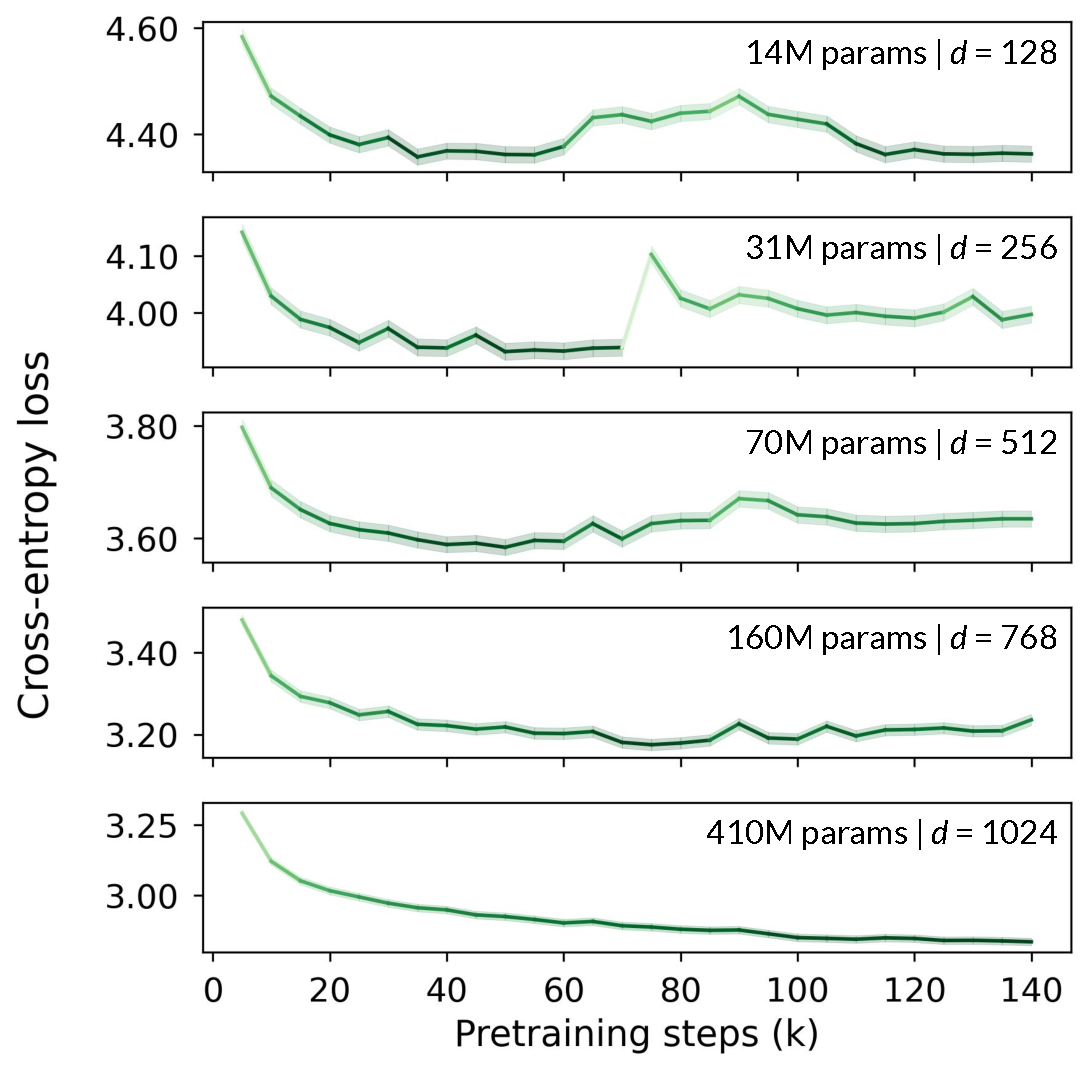
\includegraphics[width=\linewidth]{sources/part_1/softmax_bottleneck/imgs/loss_saturation_anno.pdf}
         \caption{Loss saturation}
         \label{fig:loss_sat}
    \end{subfigure}
    \begin{subfigure}{0.45\columnwidth}
         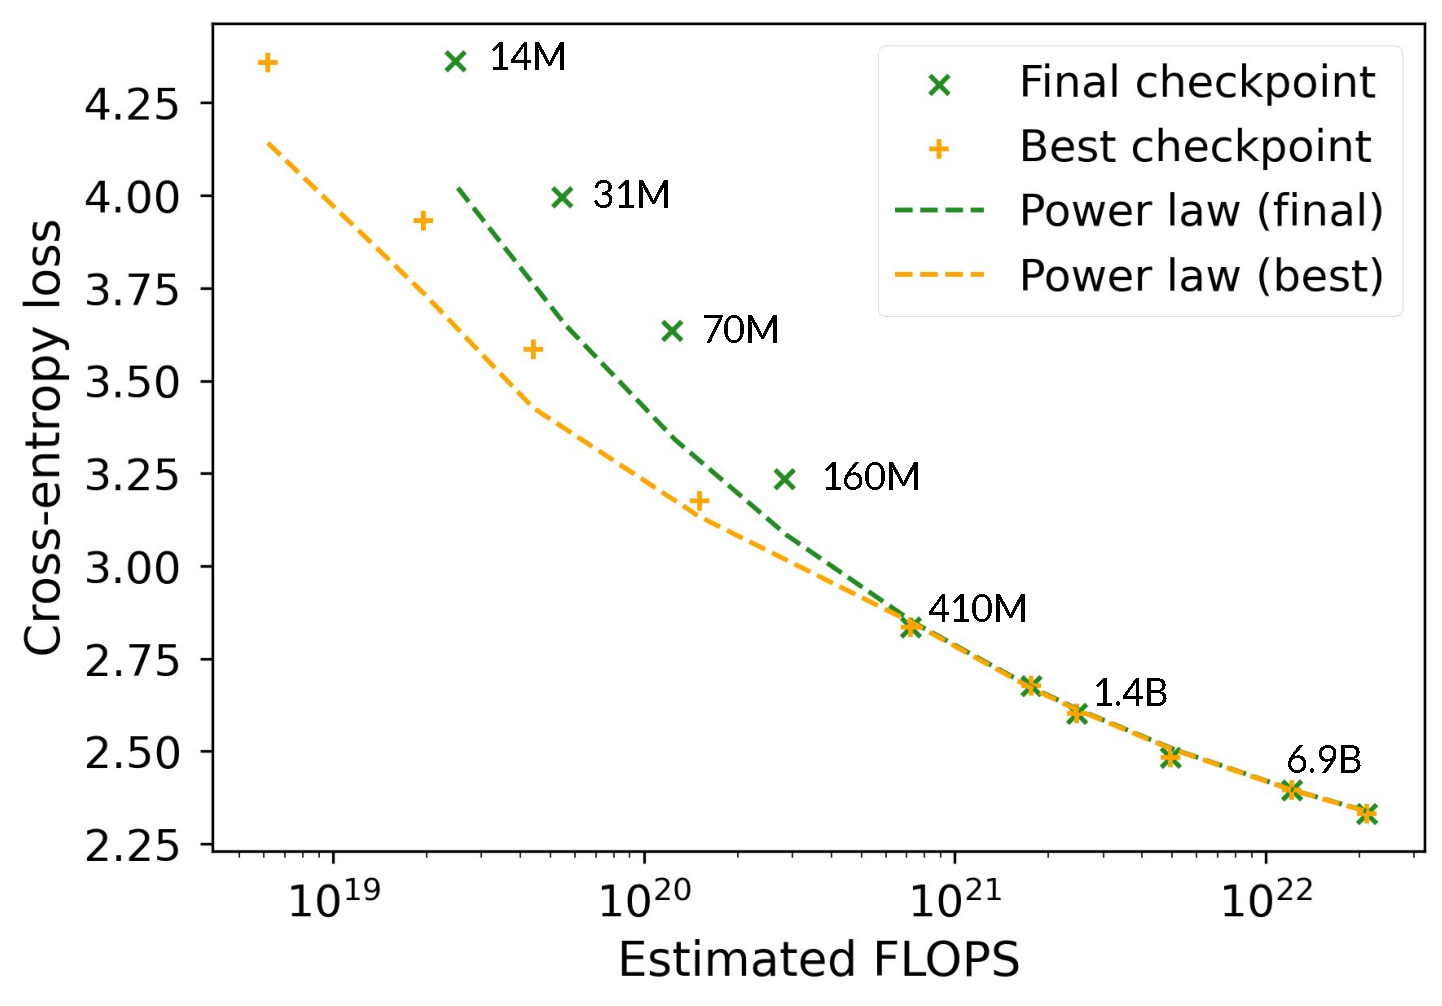
\includegraphics[width=\linewidth]{sources/part_1/softmax_bottleneck/imgs/scaling_laws_unfit_anno.pdf}
         \caption{Loss extrapolation}
         \label{fig:scaling_law}
    \end{subfigure}
    \caption{Performance of Pythia models on the Pile. On the left, we compare training dynamics of models from 14M (top) to 410M (bottom) parameters, displaying darker shades as we approach the minimal value. On the right, we fit a power law on larger models and find that final checkpoints of smaller models underperform compared to predictions.}
    \label{fig:saturation}
\end{figure}
In \Cref{fig:loss_sat}, we clearly see that models up to 410M parameters suffer from the saturation phenomenon, characterized as an increase of the in-domain loss in advanced training stages. 

In \Cref{fig:scaling_law}, we fit a scaling law in the style of \citet{chinchilla_scaling} on data points from models ranging from 410M parameters, only optimizing for model-related constants ($A$ and $\alpha$) while reusing all other values ($B=410.7$, $\beta=0.28$, $E=1.69$). We recall the relation between parameter count $N$ and token count $T$ given in \citet{chinchilla_scaling}:
$$
L(N, T) = \frac{A}{N^\alpha} + \frac{B}{T^\beta} + E
$$

We find that optimal parameters are $A=119.09$ and $\alpha=0.246$. We display the fitted curves for token counts that correspond to best and final checkpoints. We observe that the final checkpoints underperform the extrapolation by 8\% in average. The loss-minimizing (\textit{best}) checkpoints, which are expected to fall short of the extrapolation due to their incomplete learning rate cooldown, only underperform it by roughly 4\%.

We report a similar performance saturation on datasets used for evaluation using the LM Evaluation Harness \citep{eval-harness}, as shown in \Cref{tab:perf_gap}.

\begin{table}[ht]
% \scriptsize
\centering
\scalebox{0.85}{%
\begin{tabular}{@{}lcccccc@{}}
\toprule
\multicolumn{1}{c}{Checkpoint} & Lambada (ppl.) $\downarrow$ & Lambada $\uparrow$ & StoryCloze $\uparrow$ & WikiText (ppl.) $\downarrow$ & SciQ $\uparrow$ & ARC-e $\uparrow$\\ \midrule
Best & \textbf{24.6} & \textbf{40.3} & \textbf{59.6} & \textbf{30.47} & \textbf{79.6} & \textbf{46.5} \\
Final & 32.9 & 38 & 57.2 & 33.4 & 73.4 & 43.2 \\ \bottomrule
\end{tabular}}
\caption{Zero-shot performance of Pythia-160M best and final checkpoints on evaluation datasets. Unless specified, we report accuracy for all tasks.}
\label{tab:perf_gap}
\end{table}


\section{Performance Saturation is Rank Saturation}
\subsection{Anisotropy at Scale}
Given that most research on degeneration was conducted on smaller models, it remains unclear whether anisotropy affects models with over 1 billion parameters. In order to address this question, we compute average cosine-similarity of intermediate representations across layers in suites of models; namely GPT-2 \citep{gpt2}, OPT \citep{zhang2022opt}, Pythia \citep{biderman2023pythia}, and Gemma \citep{gemmateam2024gemma}. We use a subsample of The Pile \citep{gao2020pile}, as we hypothesize that the domain of this dataset includes or matches the domain of the pretraining datasets used in these suites.

\begin{figure}[ht]
    \centering
    \begin{subfigure}{0.45\columnwidth}
         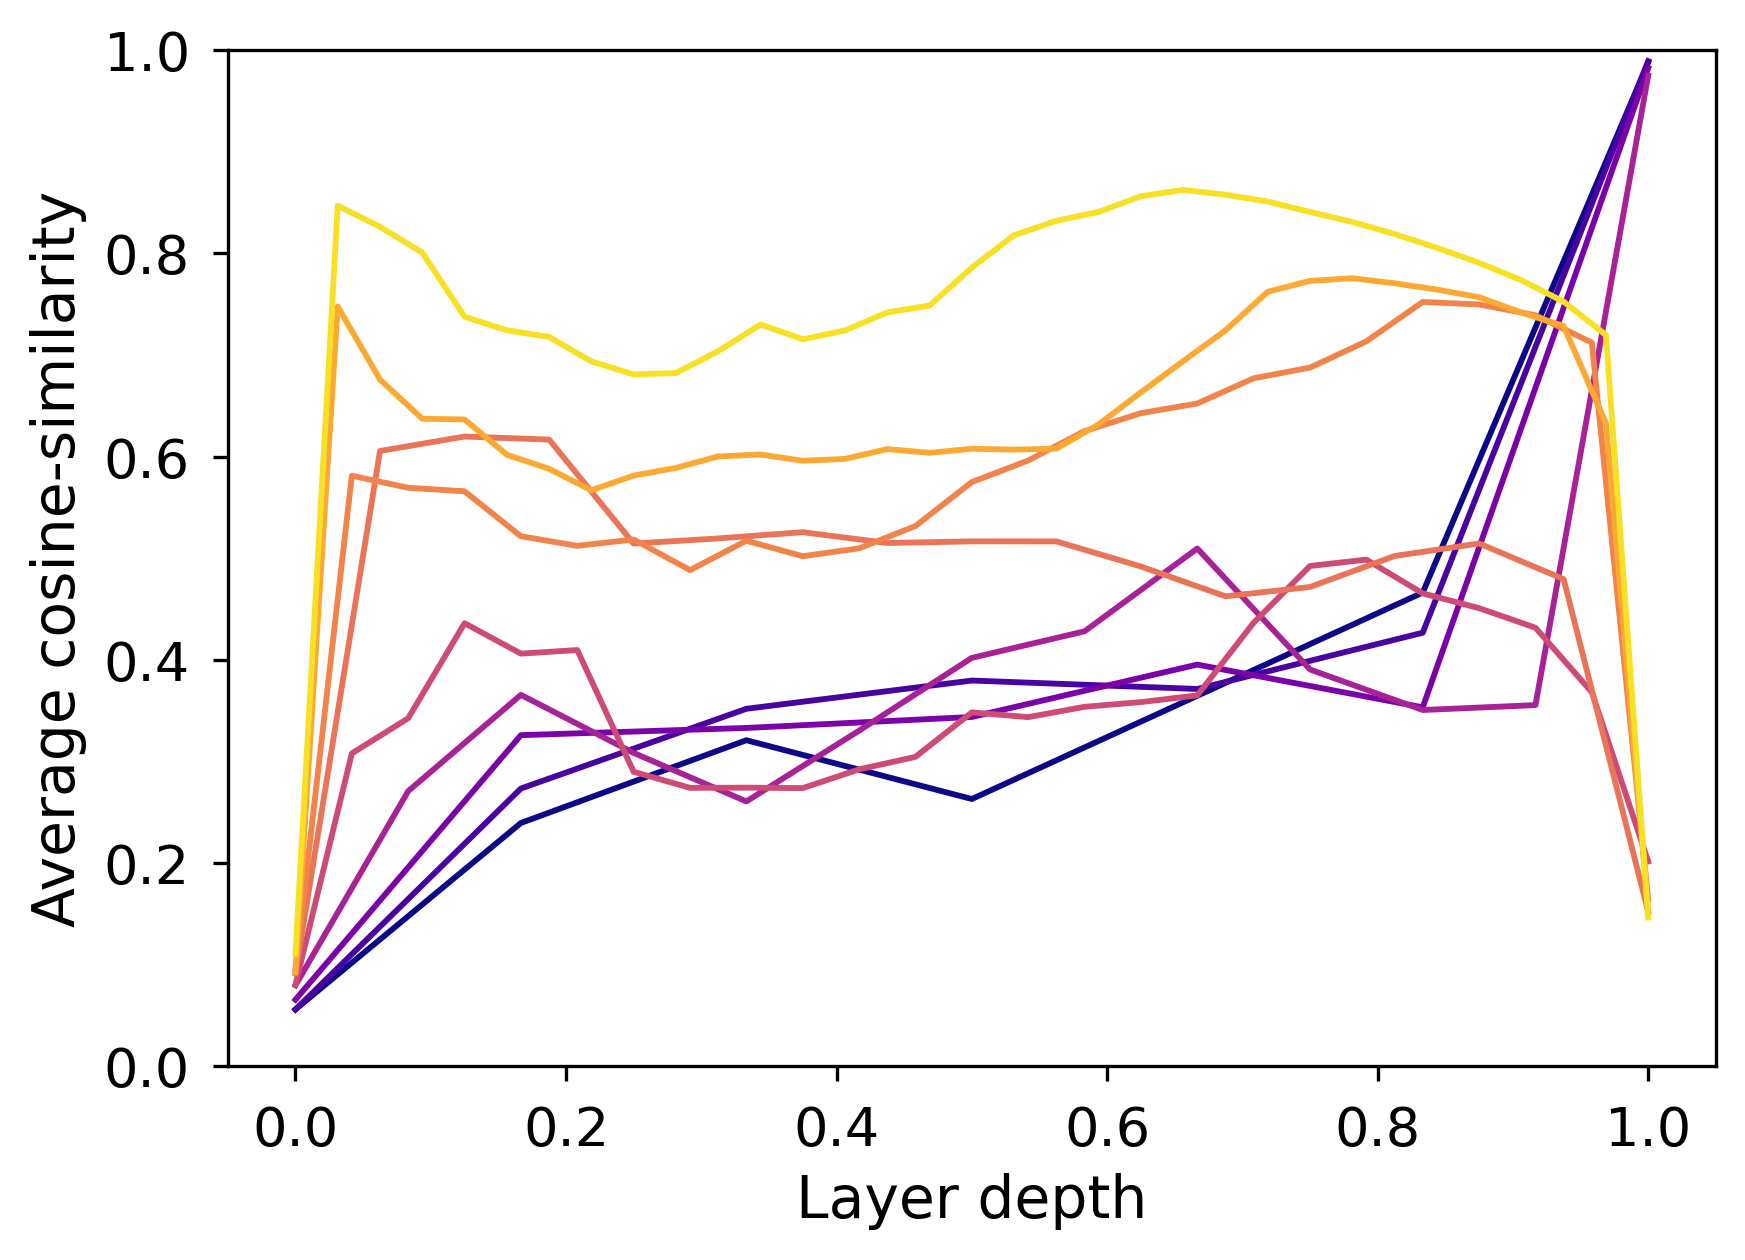
\includegraphics[width=\linewidth]{sources/part_1/softmax_bottleneck/imgs/pythia_anisotropy.png}
         \caption{Pythia}
         \label{fig:pythia_aniso}
    \end{subfigure}
    \begin{subfigure}{0.45\columnwidth}
         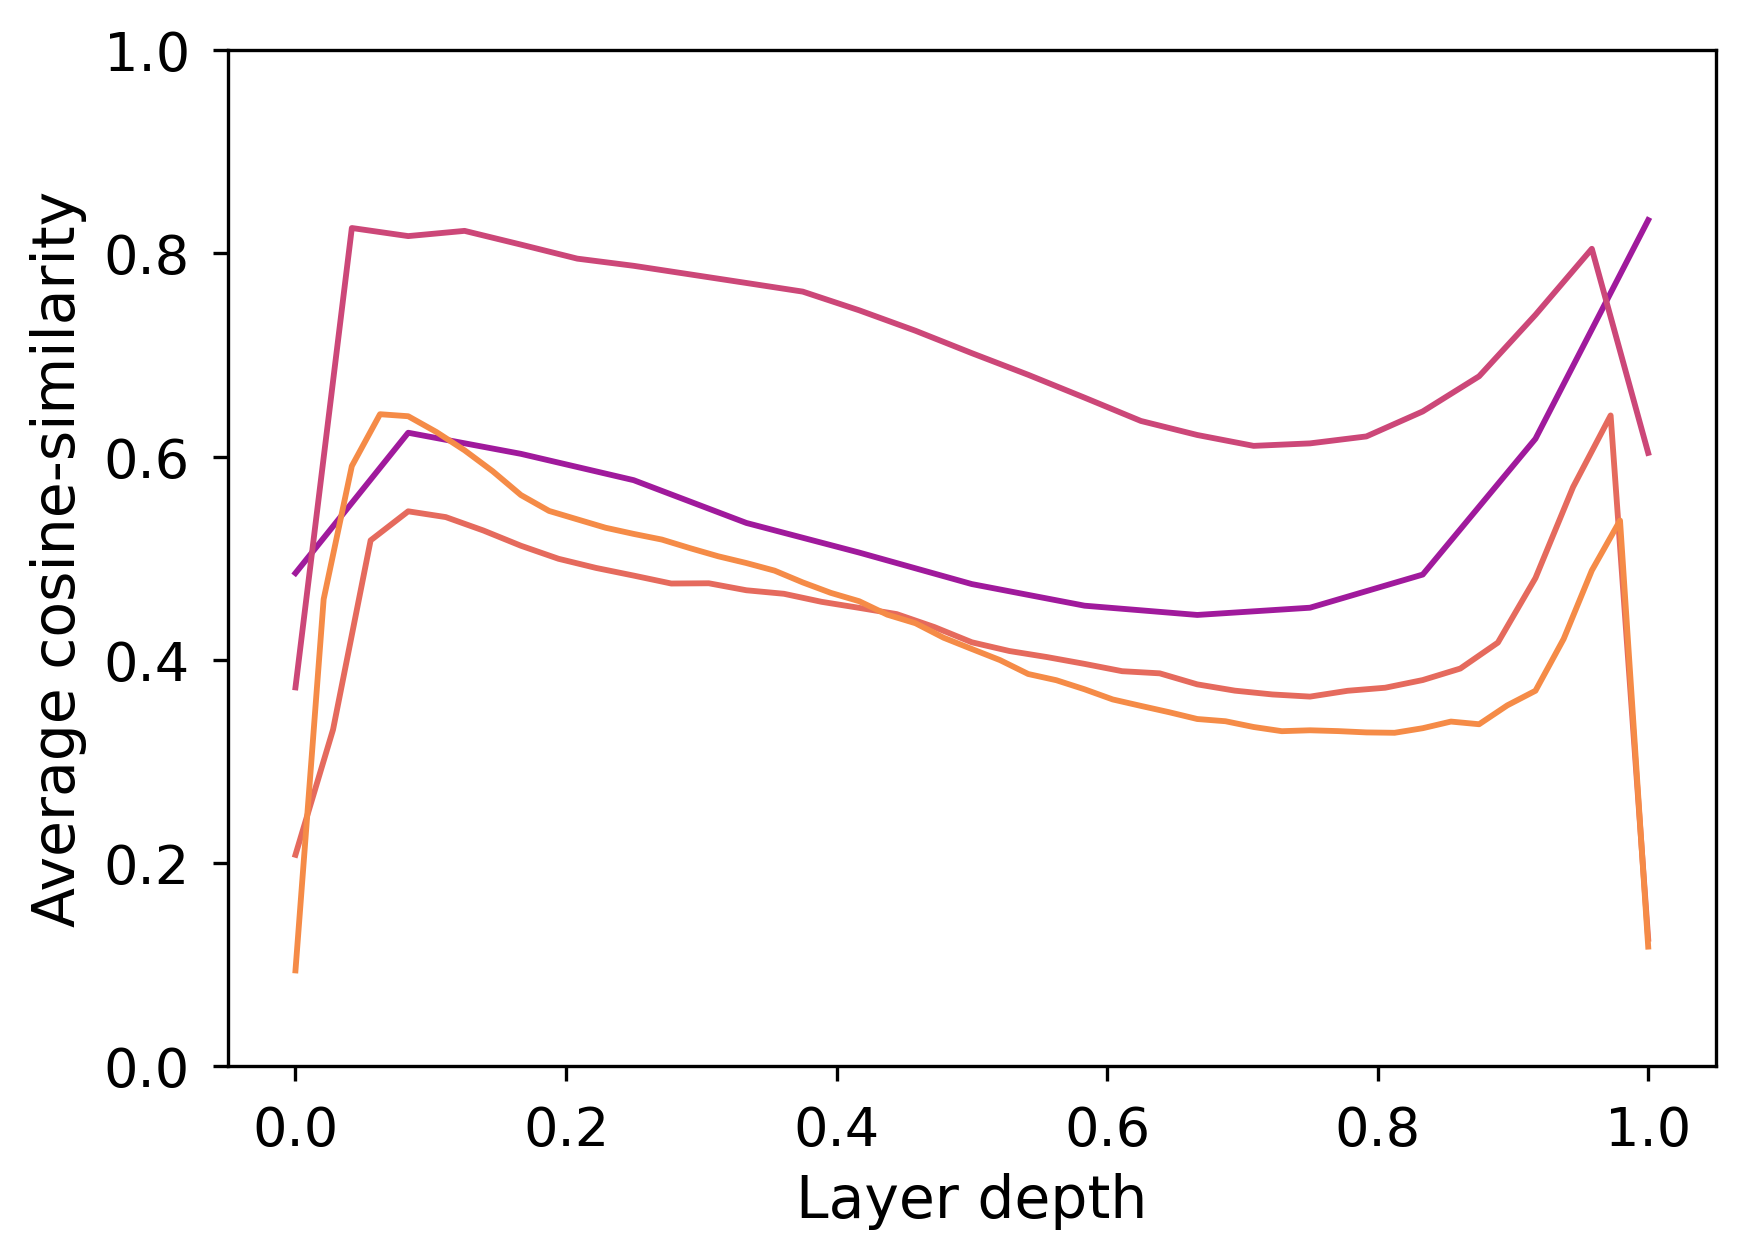
\includegraphics[width=\linewidth]{sources/part_1/softmax_bottleneck/imgs/gpt2_anisotropy.png}
         \caption{GPT-2}
         \label{fig:gpt2_aniso}
    \end{subfigure}
    \begin{subfigure}{0.45\columnwidth}
         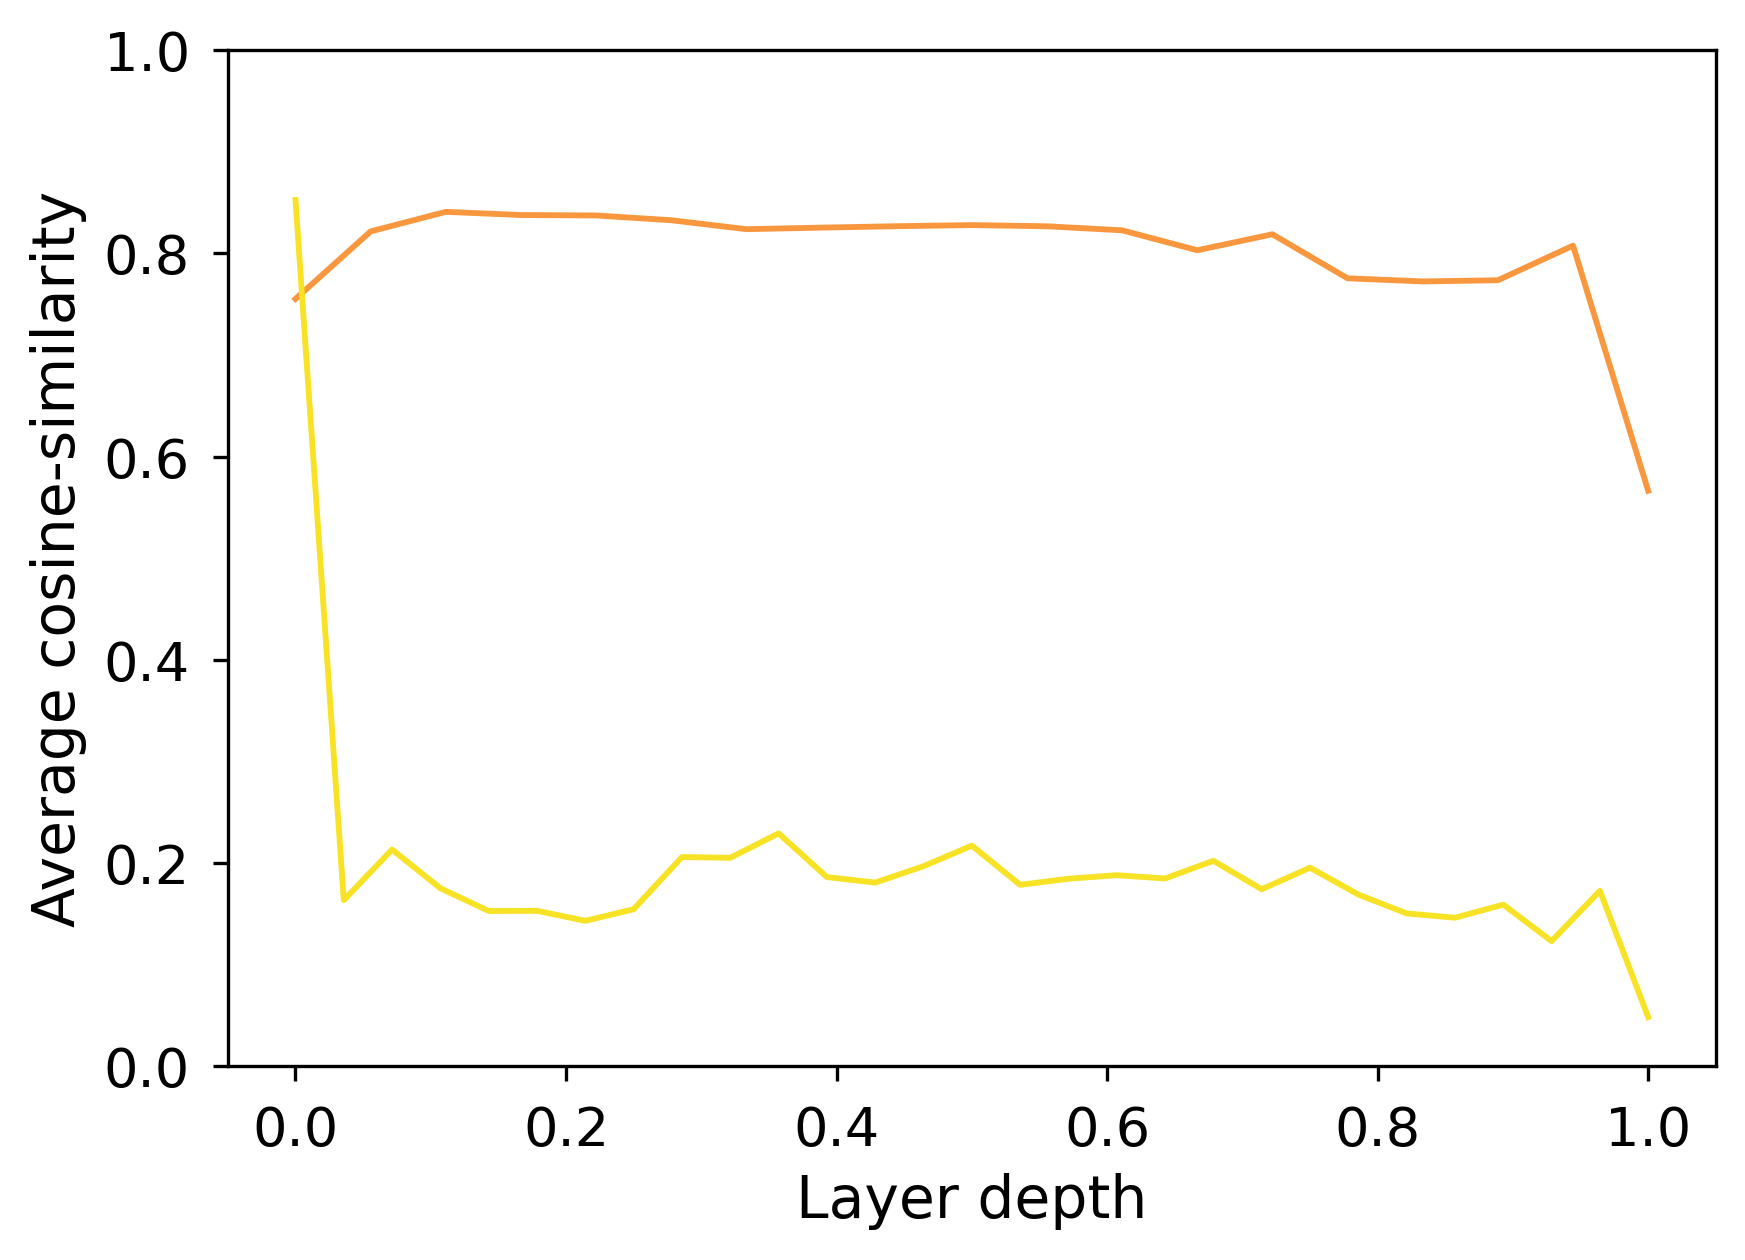
\includegraphics[width=\linewidth]{sources/part_1/softmax_bottleneck/imgs/gemma_anisotropy.png}
         \caption{Gemma}
         \label{fig:gemma_aniso}
    \end{subfigure}
    \begin{subfigure}{0.45\columnwidth}
         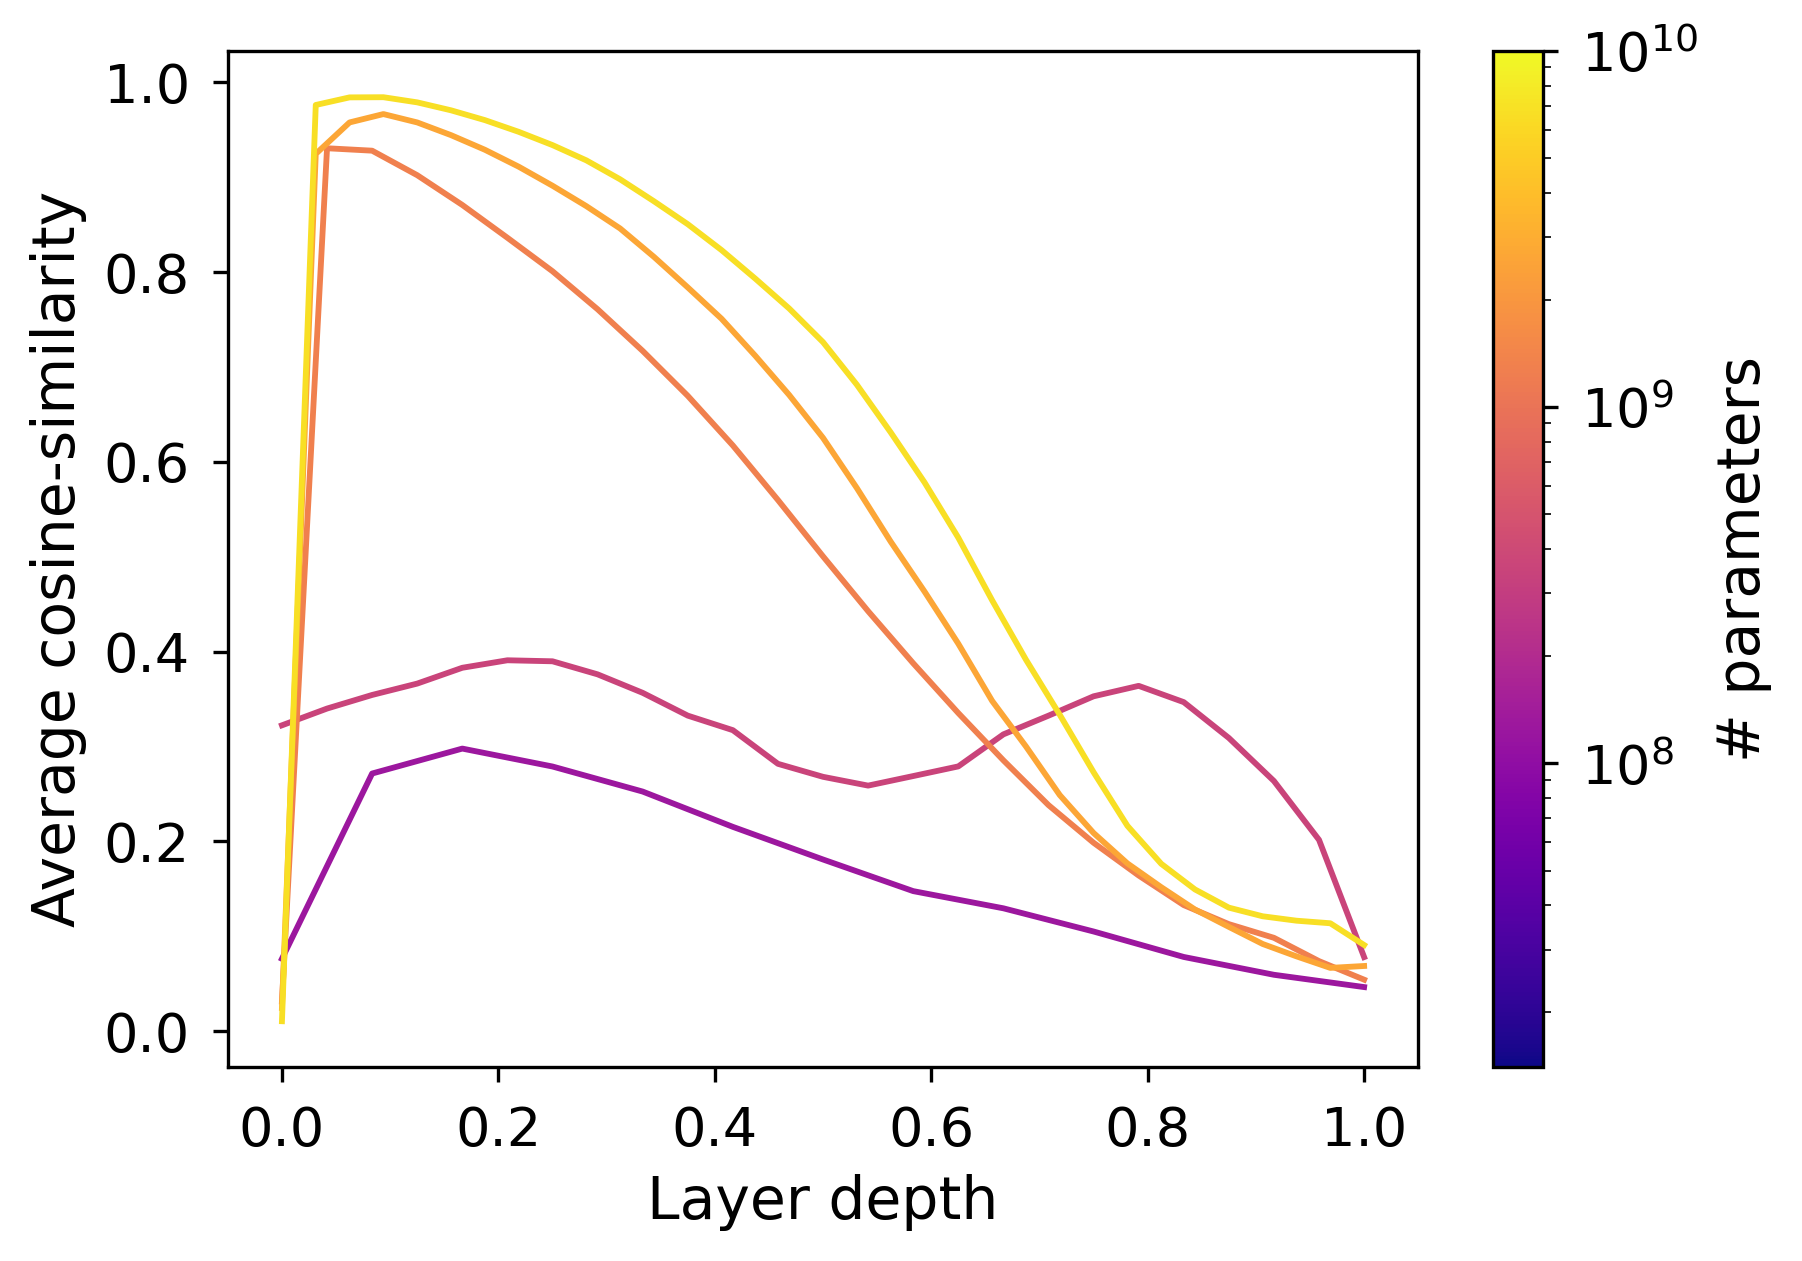
\includegraphics[width=\linewidth]{sources/part_1/softmax_bottleneck/imgs/opt_anisotropy.png}
         \caption{OPT}
         \label{fig:opt_aniso}
    \end{subfigure}
    \caption{Anisotropy in function of layer depth (i.e. order in the forward pass).}
    \label{fig:anisotropy}
\end{figure}

In \Cref{fig:anisotropy}, we observe that most layers of Transformers models are anisotropic to some extent, regardless of the scale. Nevertheless, there seems to be a dichotomy in the last layer, where models are either nearly isotropic or highly anisotropic. Interestingly, we notice that the dichotomy aligns with the one of the saturation phenomenon for the Pythia suite, where only models containing 160M or fewer parameters seem affected by last-layer anisotropy. In this chapter, we will focus on last-layer anisotropy, and we refer to \Cref{chap:anisotropy} for a study of degeneration in intermediate layers.

We thus decide to study the training dynamics of anisotropy for the Pythia suite, and compare them with the saturation phenomenon in \Cref{fig:aniso_v_saturation}.

\begin{figure}[ht!]
    \centering
    \begin{subfigure}{0.45\columnwidth}
         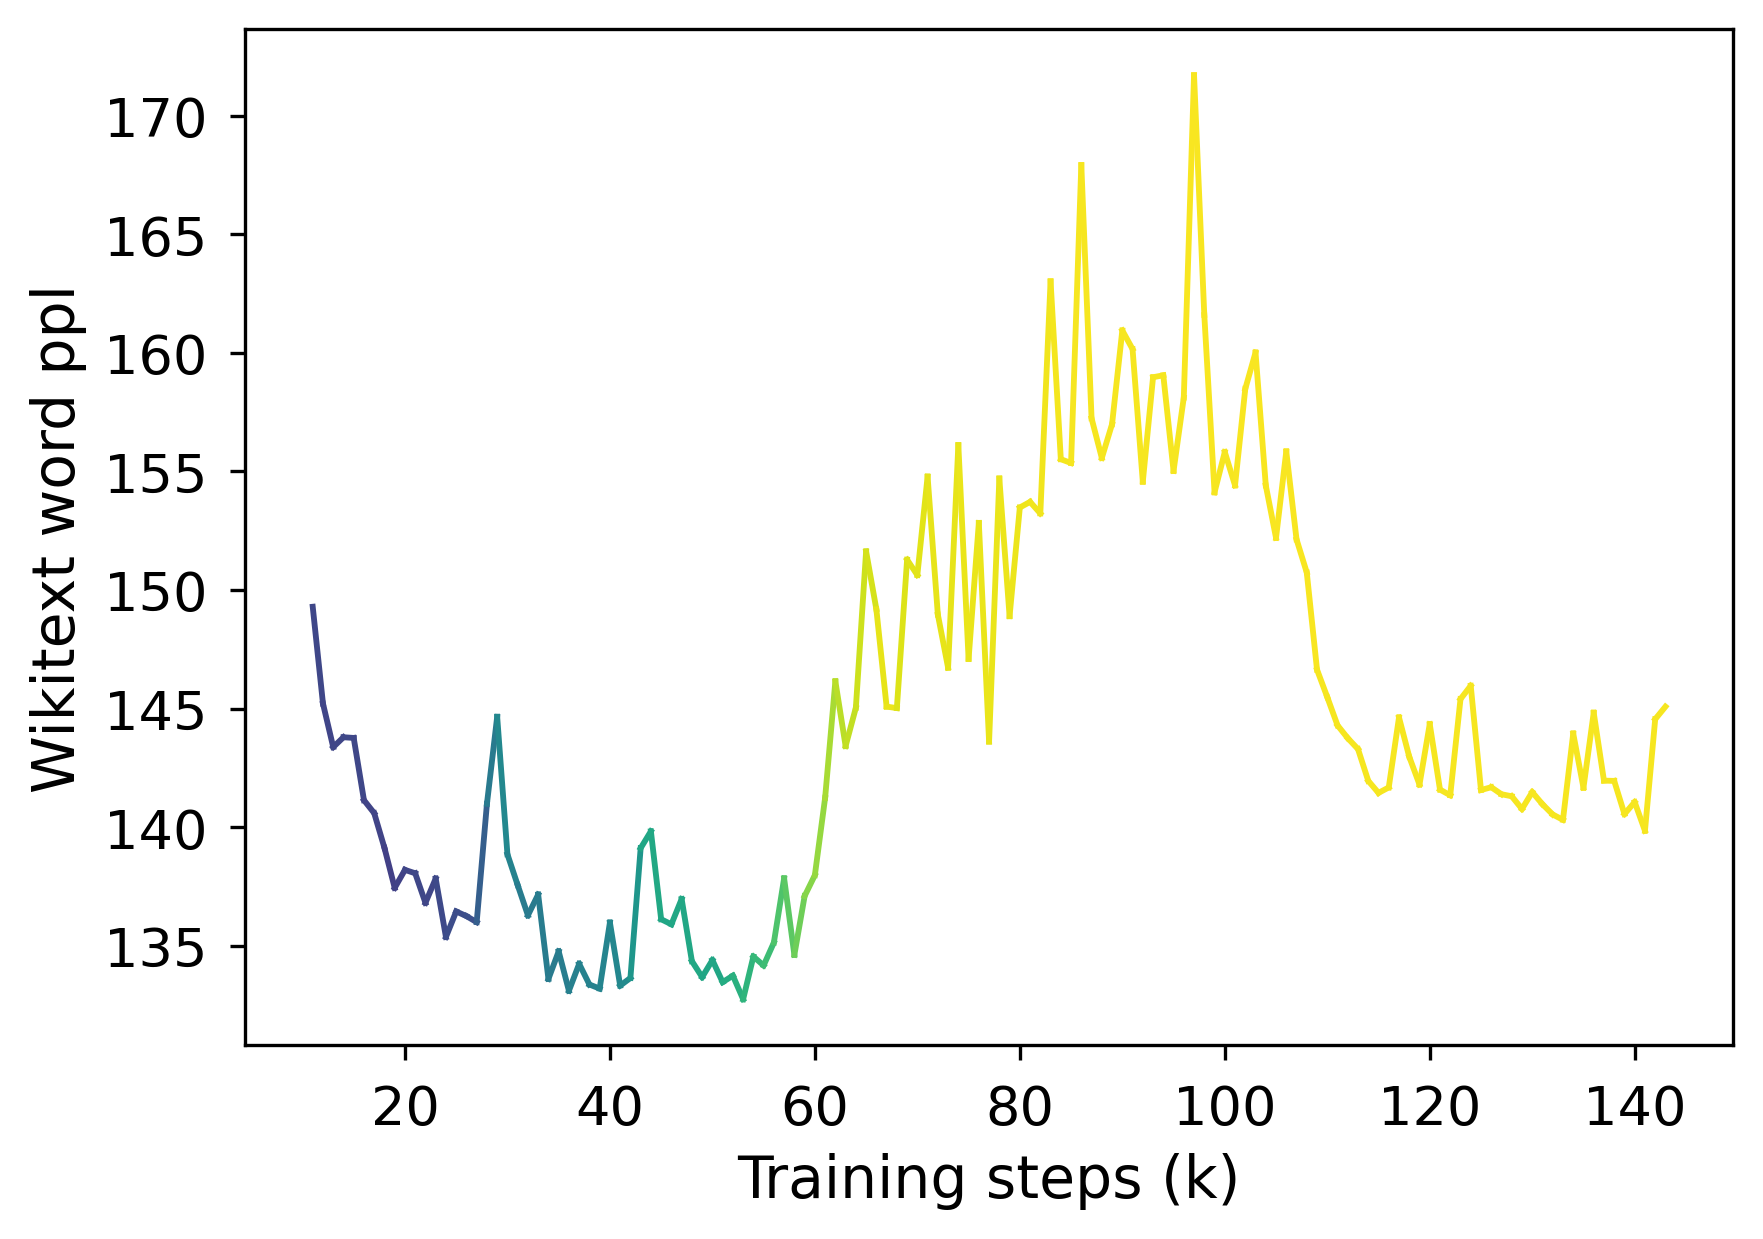
\includegraphics[width=\linewidth]{sources/part_1/softmax_bottleneck/imgs/anisotropy_explosion_14m.png}
         \caption{14M}
         \label{fig:14M}
    \end{subfigure}
    \begin{subfigure}{0.45\columnwidth}
         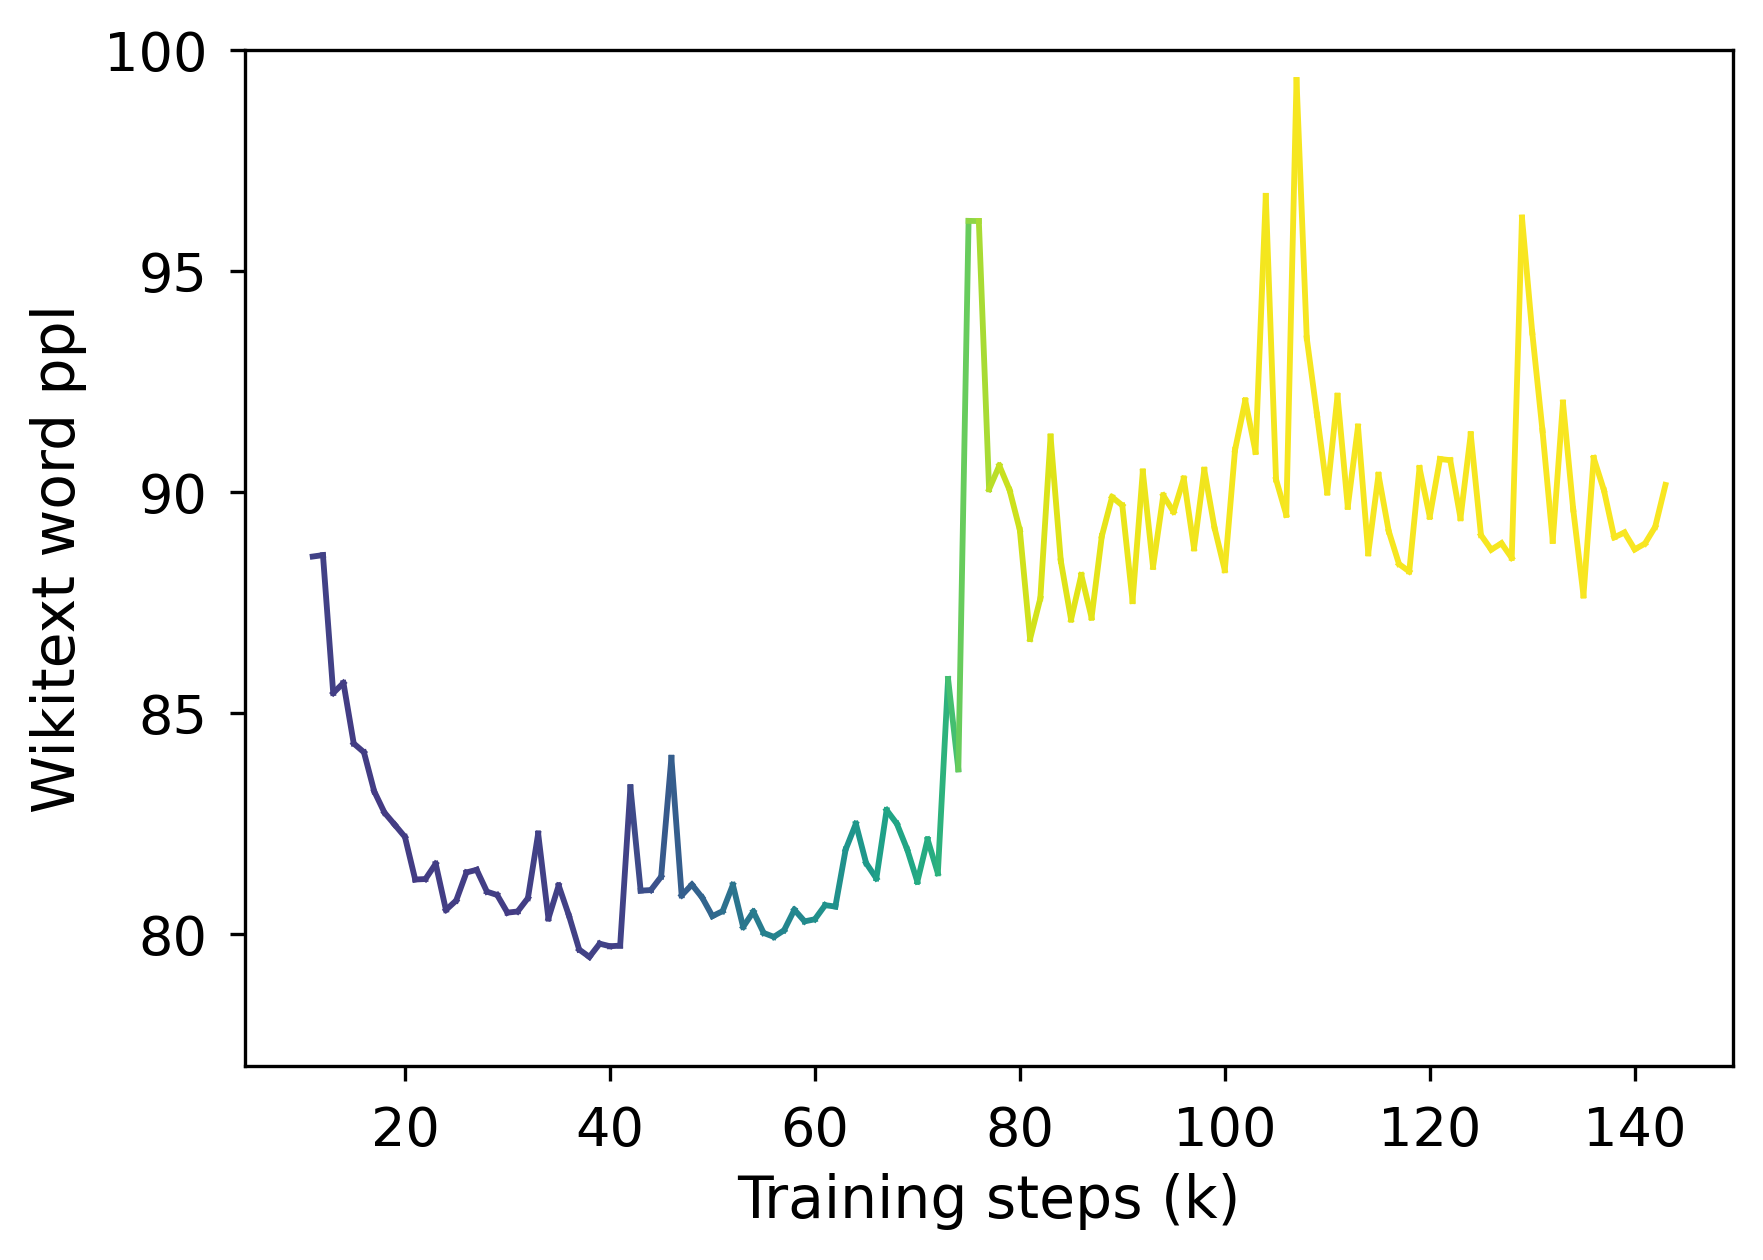
\includegraphics[width=\linewidth]{sources/part_1/softmax_bottleneck/imgs/anisotropy_explosion_31m.png}
         \caption{31M}
         \label{fig:31M}
    \end{subfigure}
    \begin{subfigure}{0.45\columnwidth}
         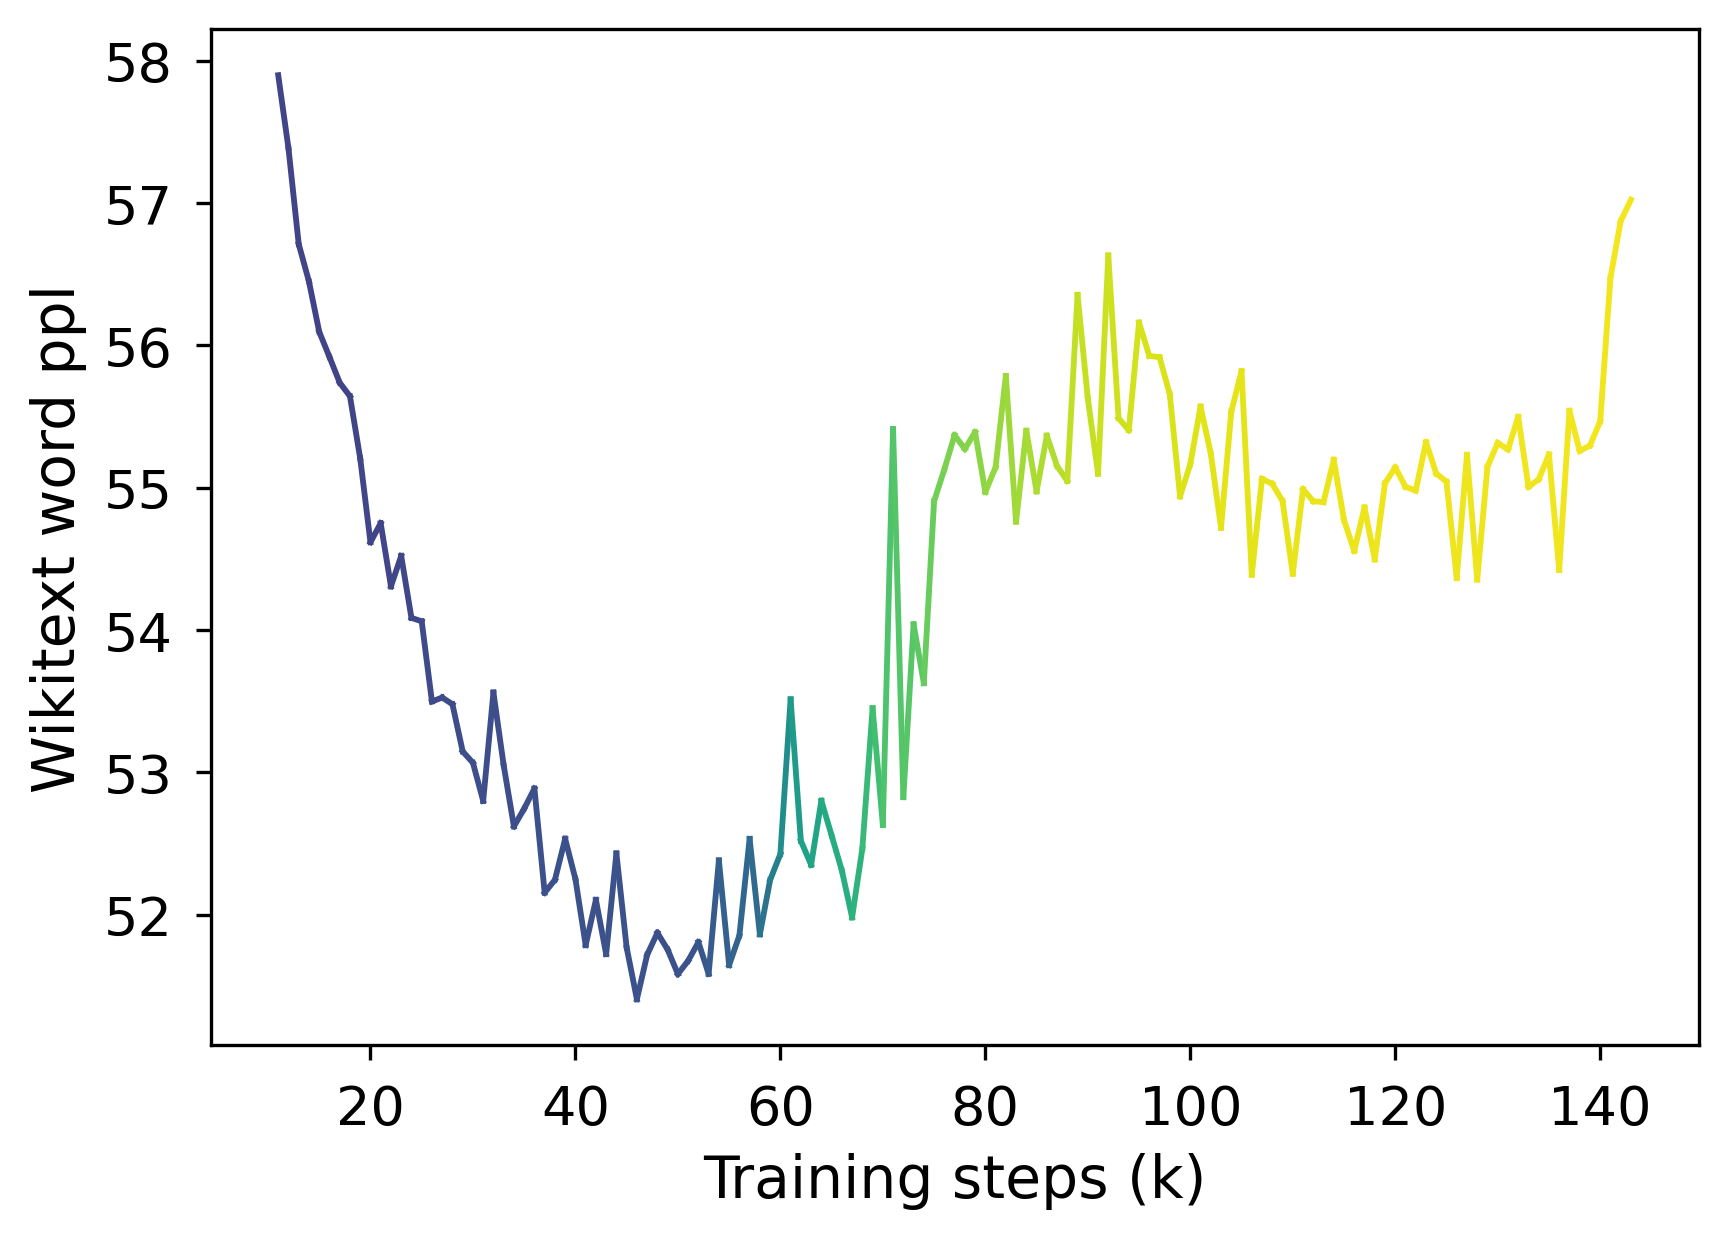
\includegraphics[width=\linewidth]{sources/part_1/softmax_bottleneck/imgs/anisotropy_explosion_70m.png}
         \caption{70M}
         \label{fig:70M}
    \end{subfigure}
    \begin{subfigure}{0.45\columnwidth}
         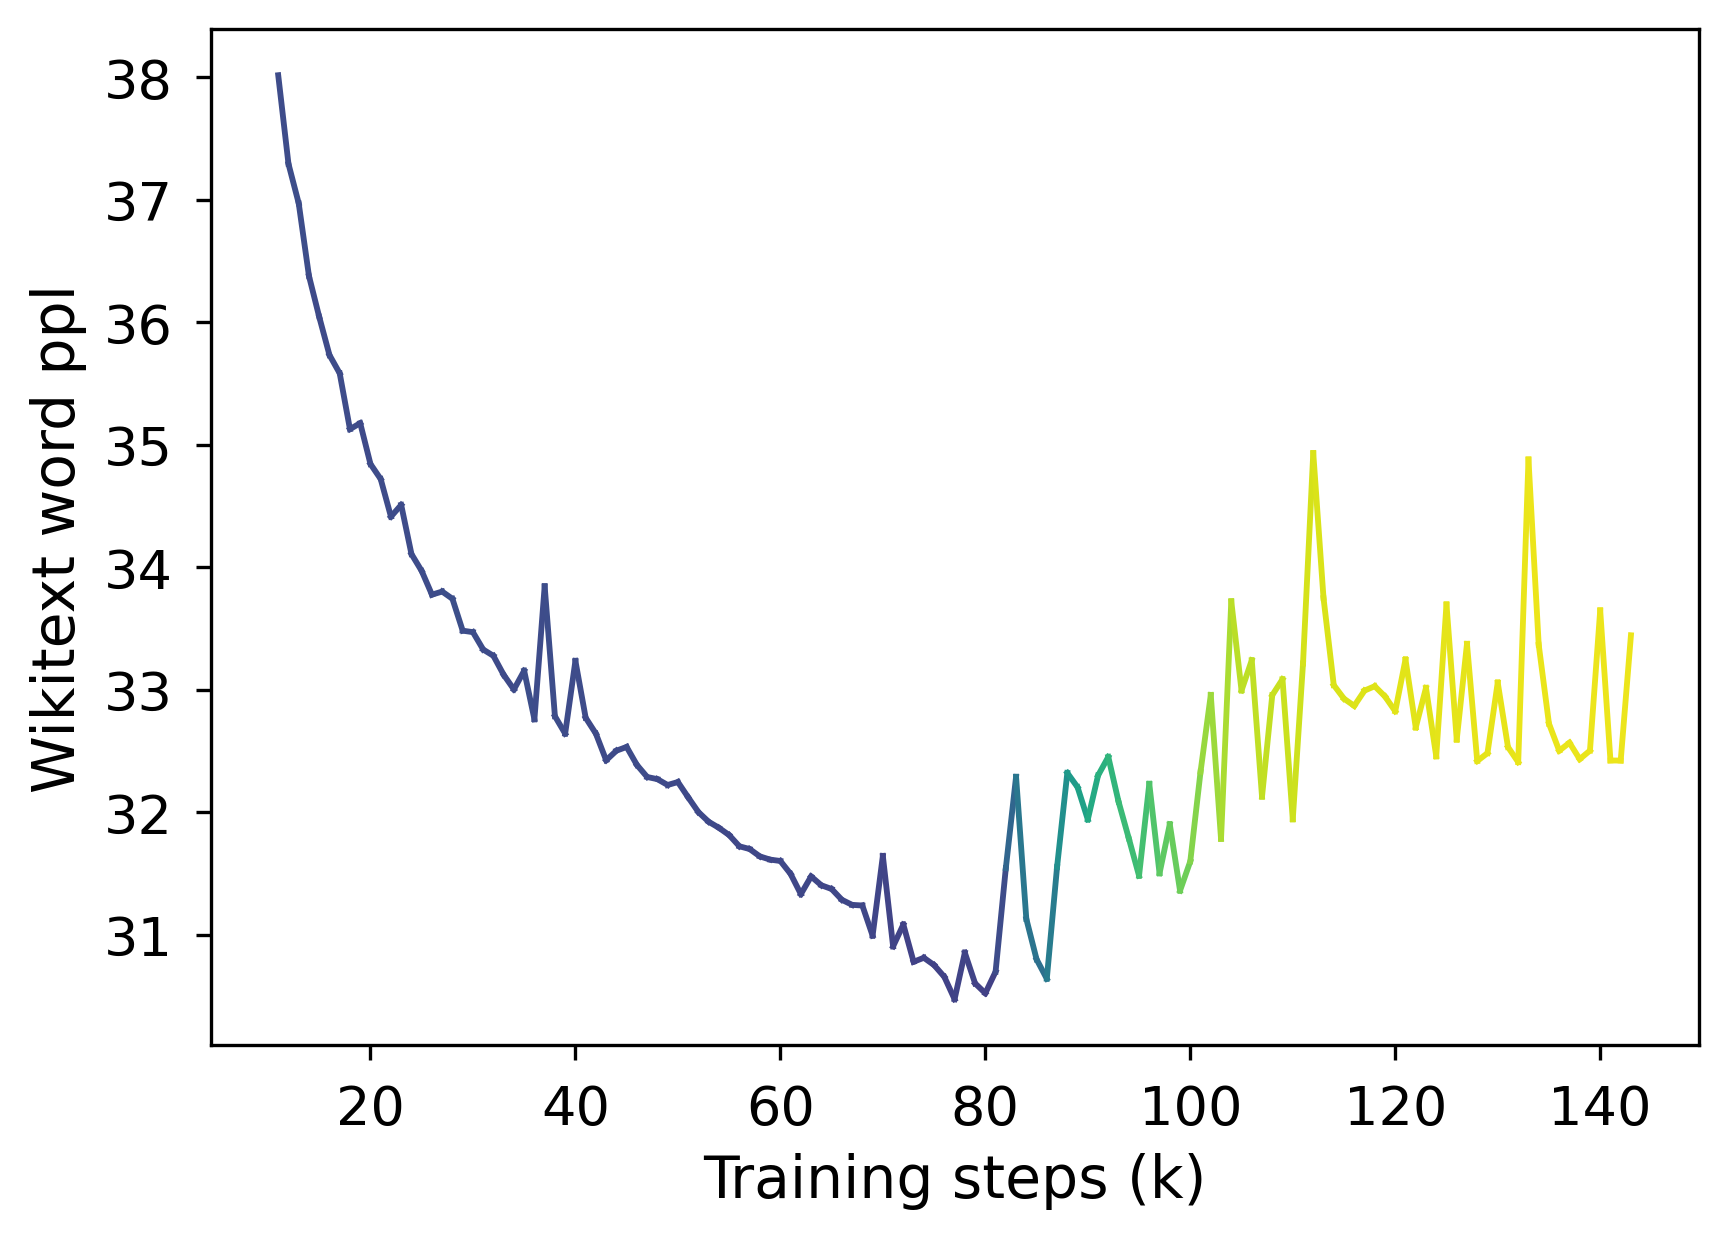
\includegraphics[width=\linewidth]{sources/part_1/softmax_bottleneck/imgs/anisotropy_explosion_160m.png}
         \caption{160M}
         \label{fig:160M}
    \end{subfigure}
    \begin{subfigure}{0.45\columnwidth}
         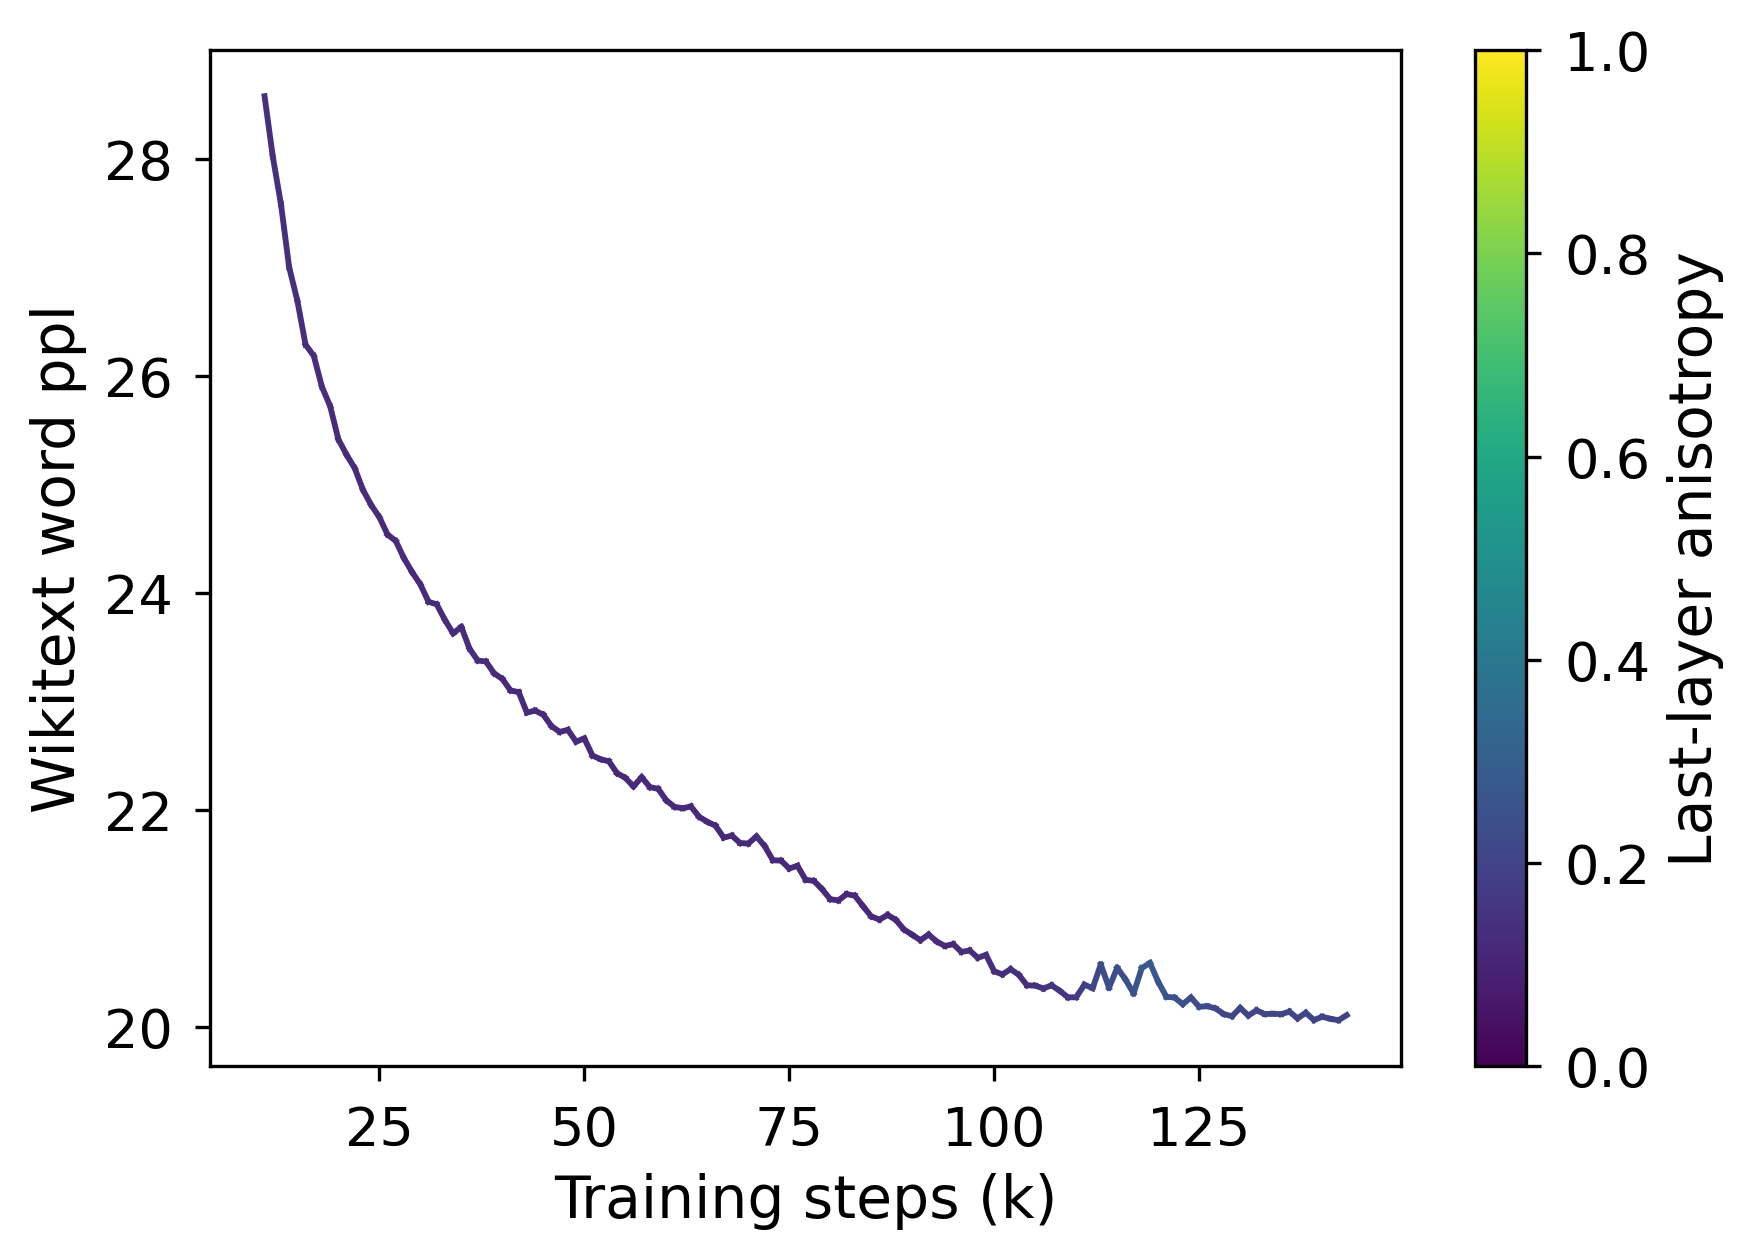
\includegraphics[width=\linewidth]{sources/part_1/softmax_bottleneck/imgs/anisotropy_explosion_410m.png}
         \caption{410M}
         \label{fig:410M}
    \end{subfigure}
    \caption{Evolution of the language modeling performance on the Wikipedia test set from the LM Evaluation Harness \citep{eval-harness} and last-layer anisotropy of Pythia models along training (color).}
    \label{fig:aniso_v_saturation}
\end{figure}

\Cref{fig:aniso_v_saturation} illustrates a neat correlation between the emergence of the performance saturation phenomenon and the appearance of anisotropy in the last-layer representations of the models. It also shows that anisotropy increases abruptly around the saturation point during training. Moreover, we see here that on a specific in-domain corpus, the models quickly lose performance at saturation and never seem to fully recover from this explosion.

\subsection{Singular Values Saturation}
\label{sub:saturation}

Average cosine-similarity is a valuable measure of the uniformity of a distribution, but including other metrics can help to better capture the complexity of some manifolds \citep{rudman-etal-2022-isoscore}. Moreover, it only focuses on the output embeddings of the language models, and not on their weights. In this section, we extend our analysis by studying the singular value distributions of the language modeling heads, to link our empirical observations to our theoretical findings. In \Cref{fig:sv_evolve}, we display the singular value distributions of the final predictive layer weights $W$ along training.

\begin{figure}[ht!]
    \centering
    \begin{subfigure}{0.45\columnwidth}
         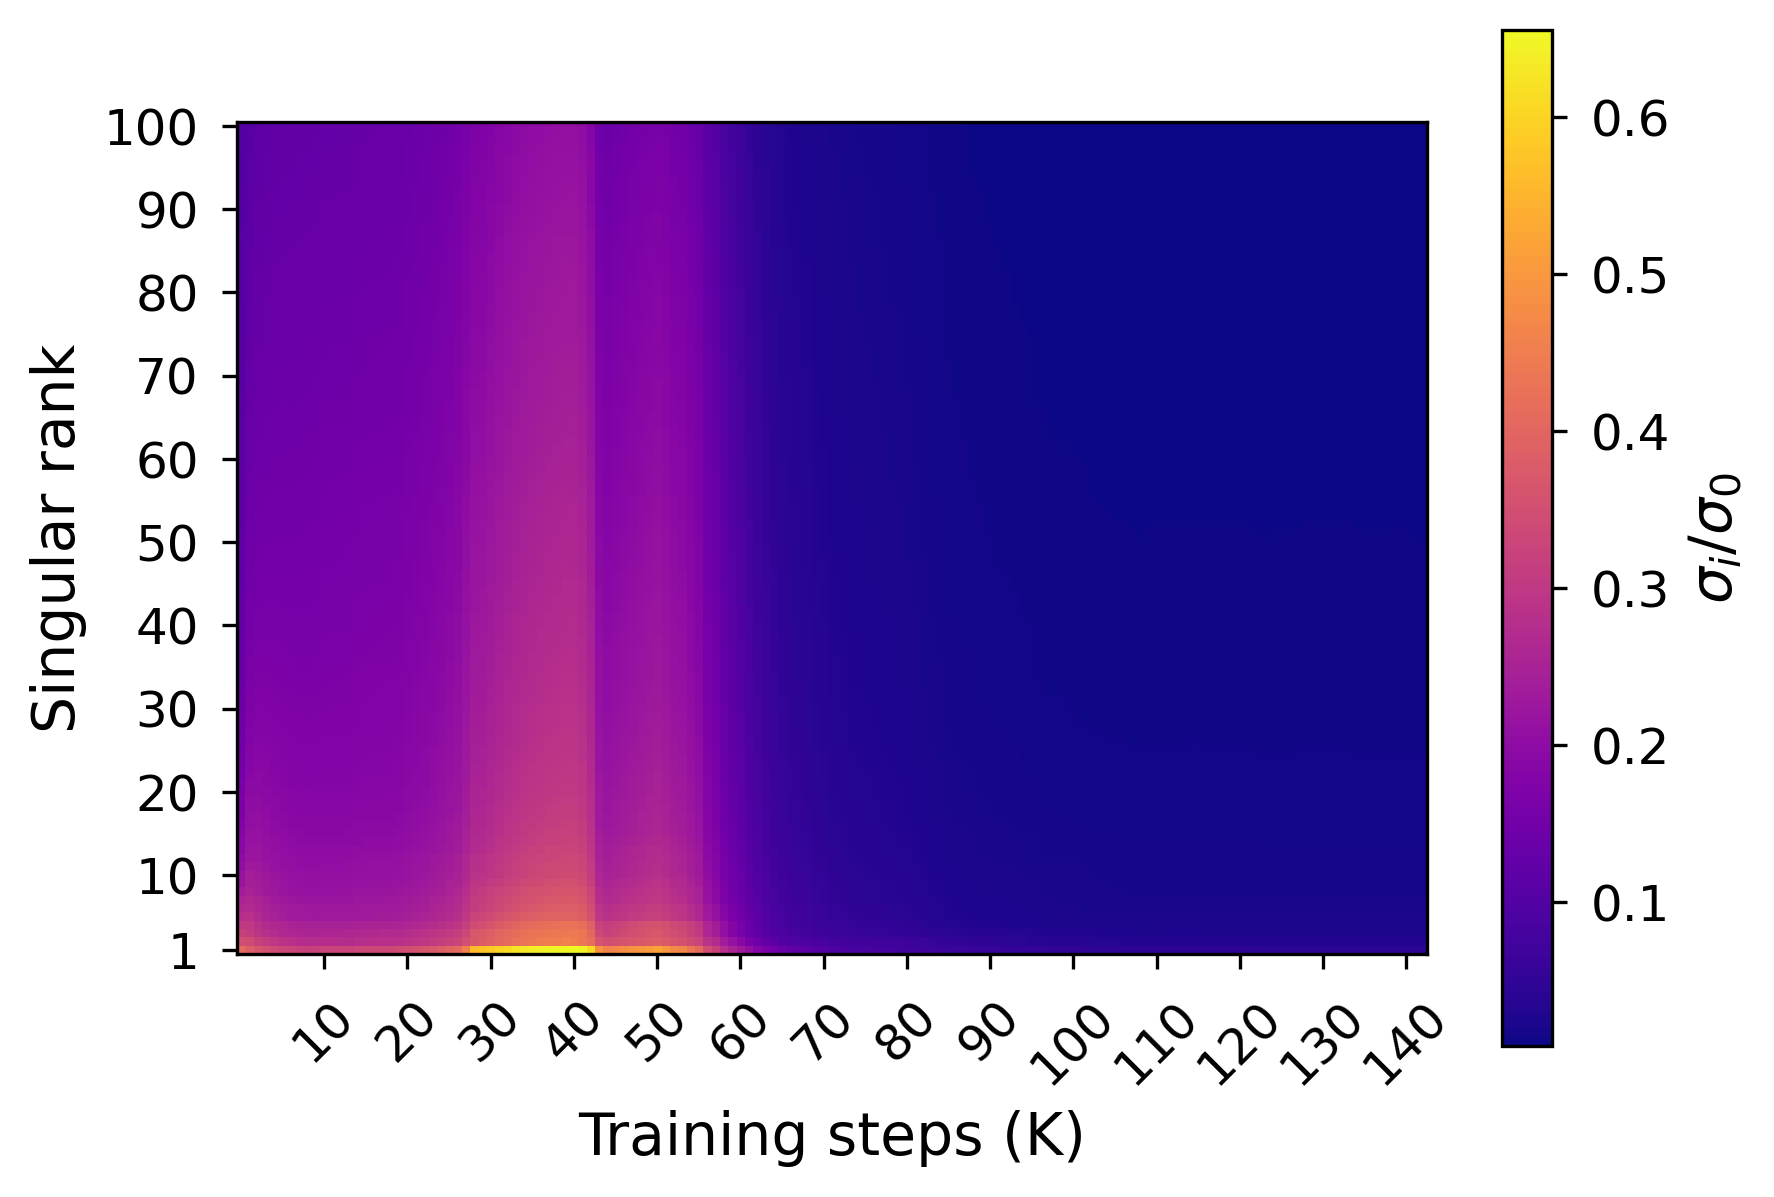
\includegraphics[width=\linewidth]{sources/part_1/softmax_bottleneck/imgs/sv_map_14m.png}
         \caption{14M}
         \label{fig:sv_14M}
    \end{subfigure}
    \begin{subfigure}{0.45\columnwidth}
         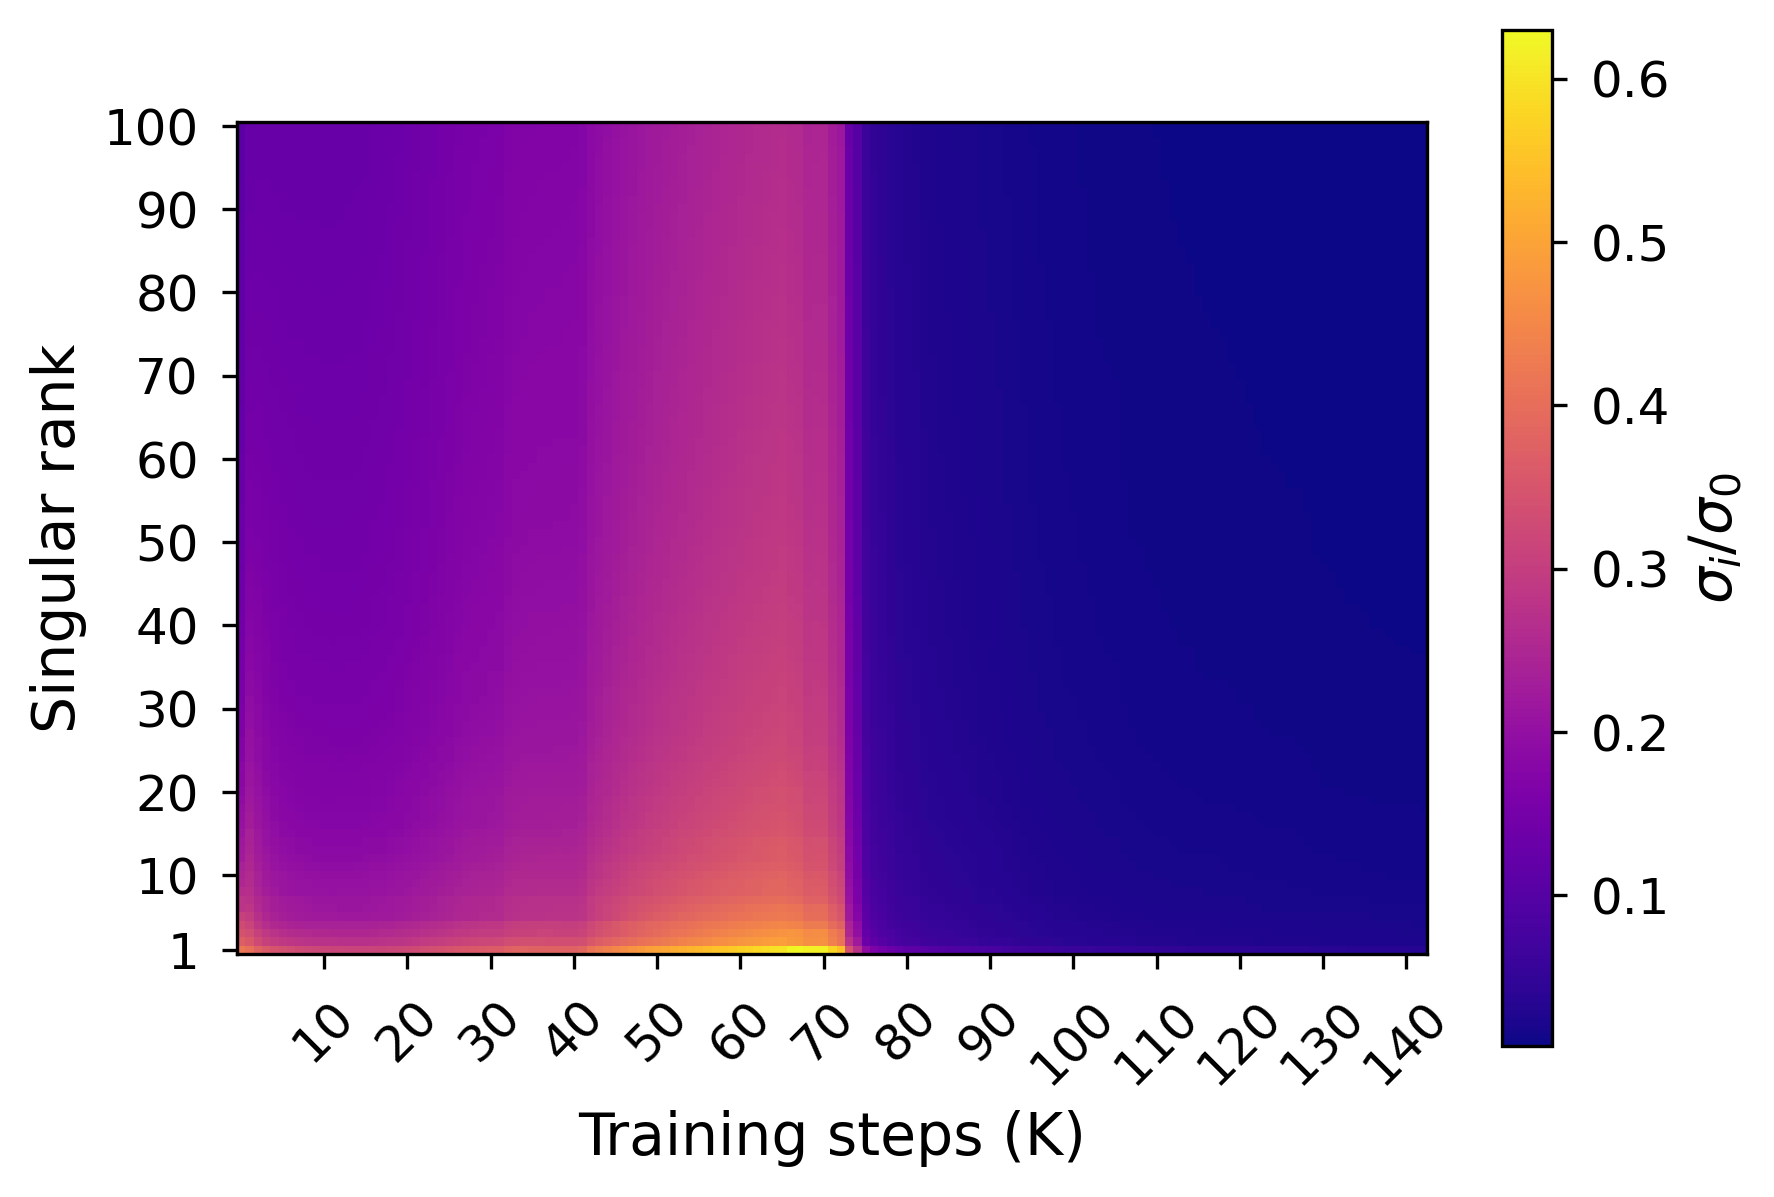
\includegraphics[width=\linewidth]{sources/part_1/softmax_bottleneck/imgs/sv_map_31m.png}
         \caption{31M}
         \label{fig:sv_31M}
    \end{subfigure}
    \begin{subfigure}{0.45\columnwidth}
         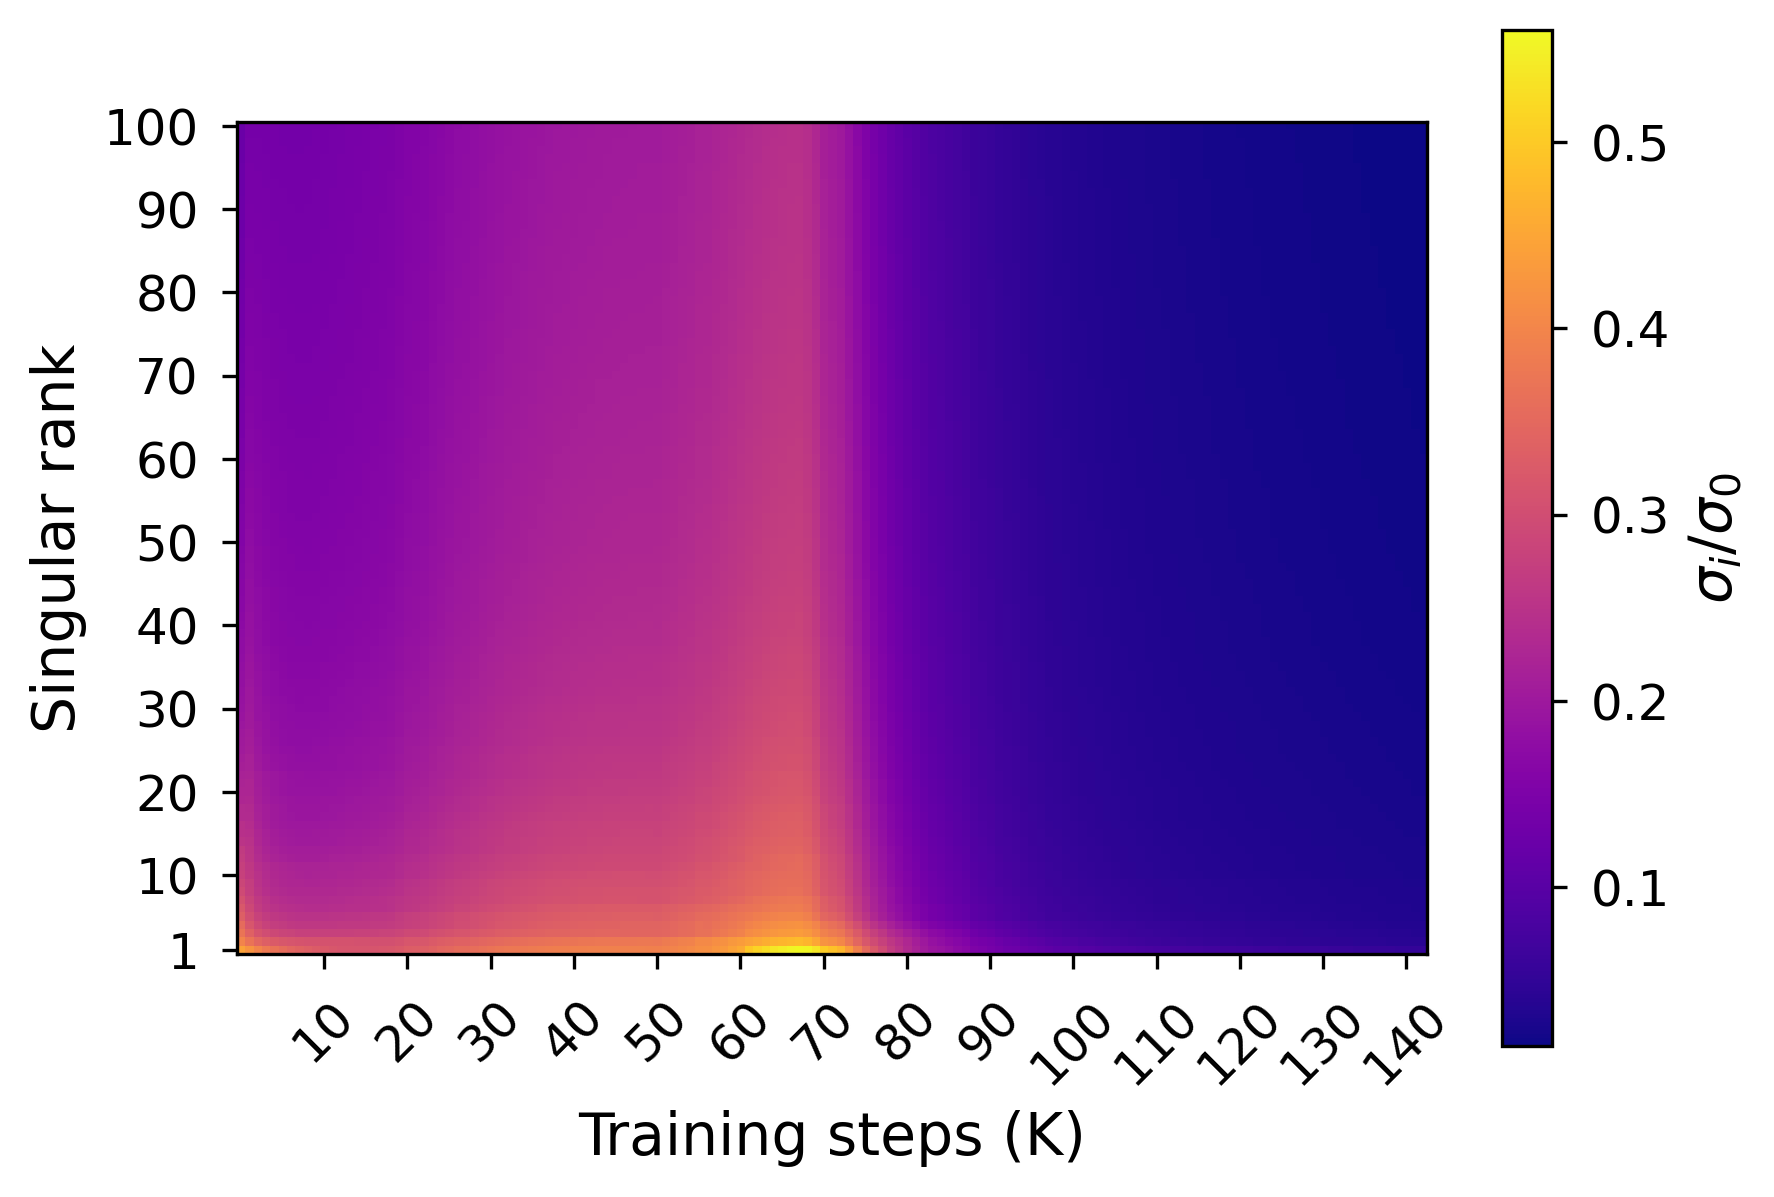
\includegraphics[width=\linewidth]{sources/part_1/softmax_bottleneck/imgs/sv_map_70m.png}
         \caption{70M}
         \label{fig:sv_70M}
    \end{subfigure}
    \begin{subfigure}{0.45\columnwidth}
         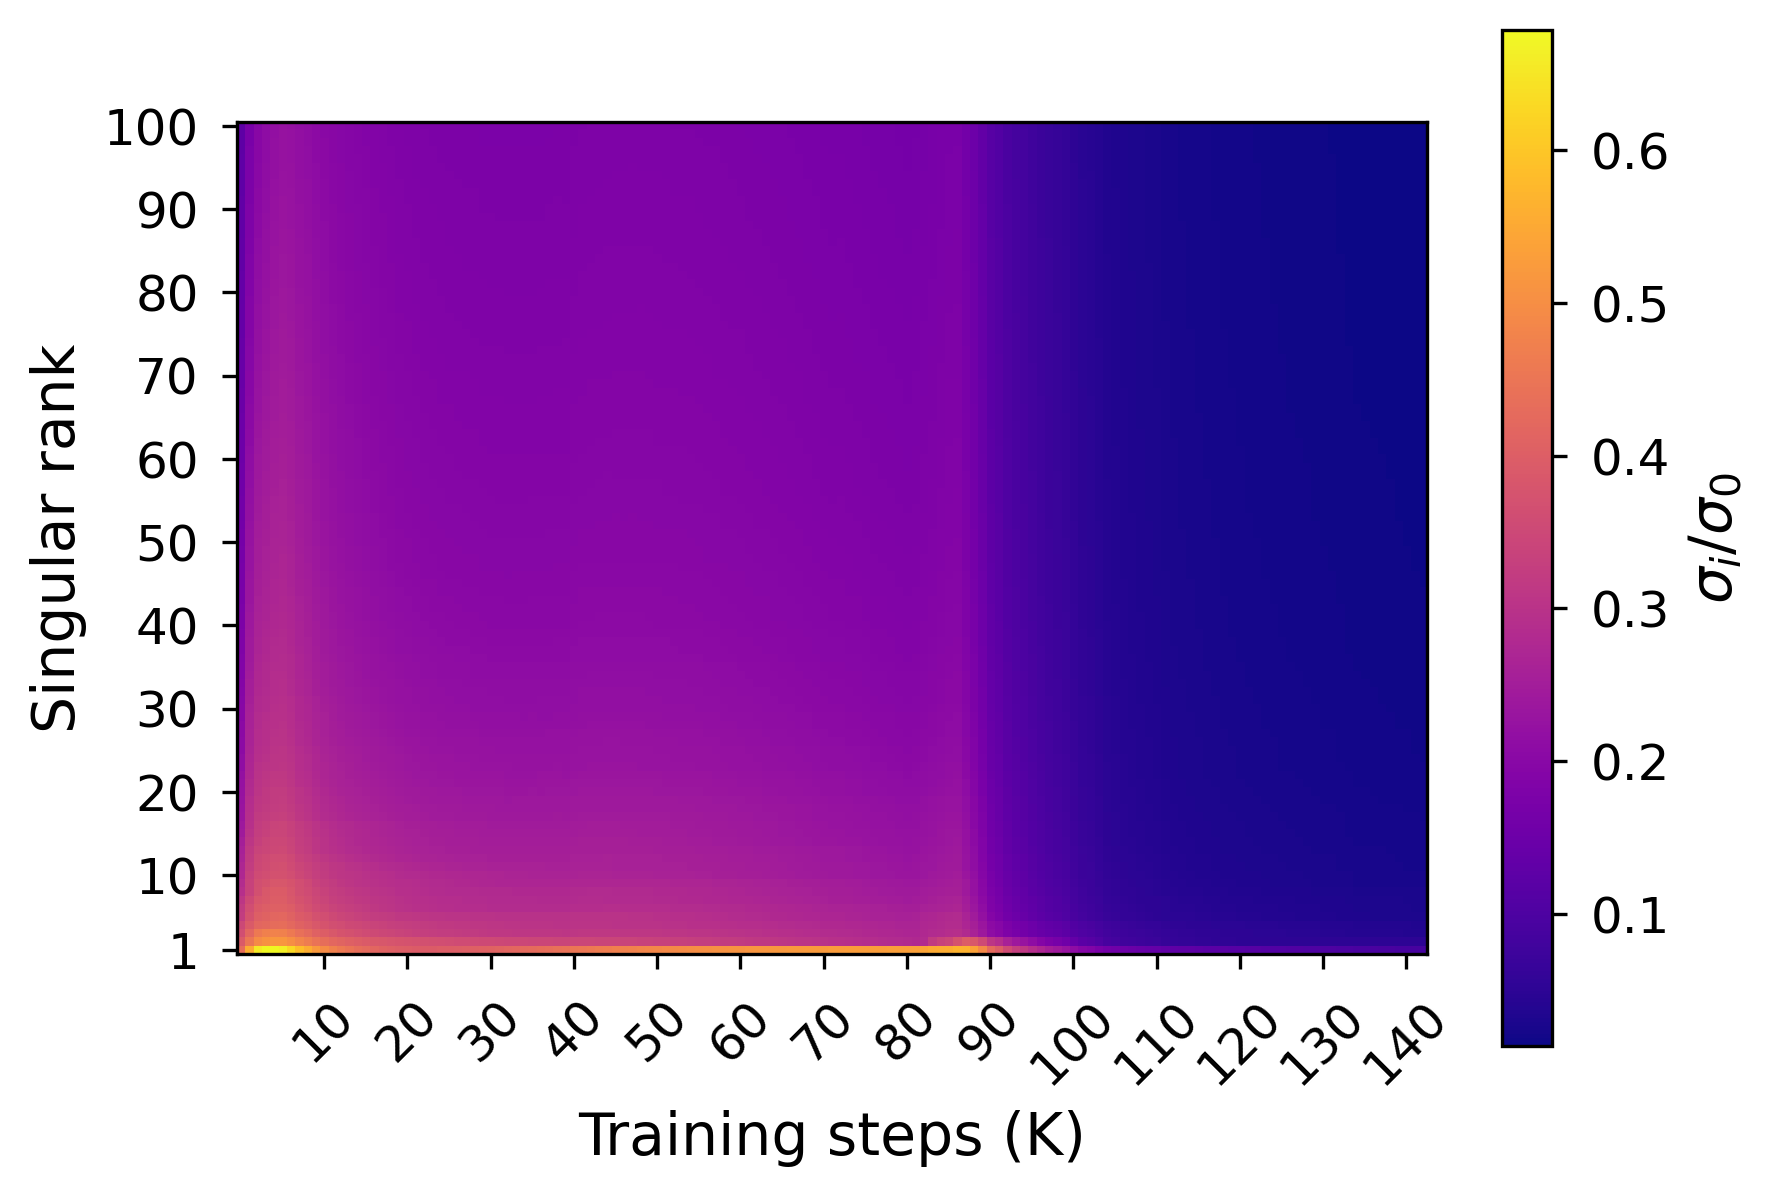
\includegraphics[width=\linewidth]{sources/part_1/softmax_bottleneck/imgs/sv_map_160m.png}
         \caption{160M}
         \label{fig:sv_160M}
    \end{subfigure}
    \begin{subfigure}{0.45\columnwidth}
         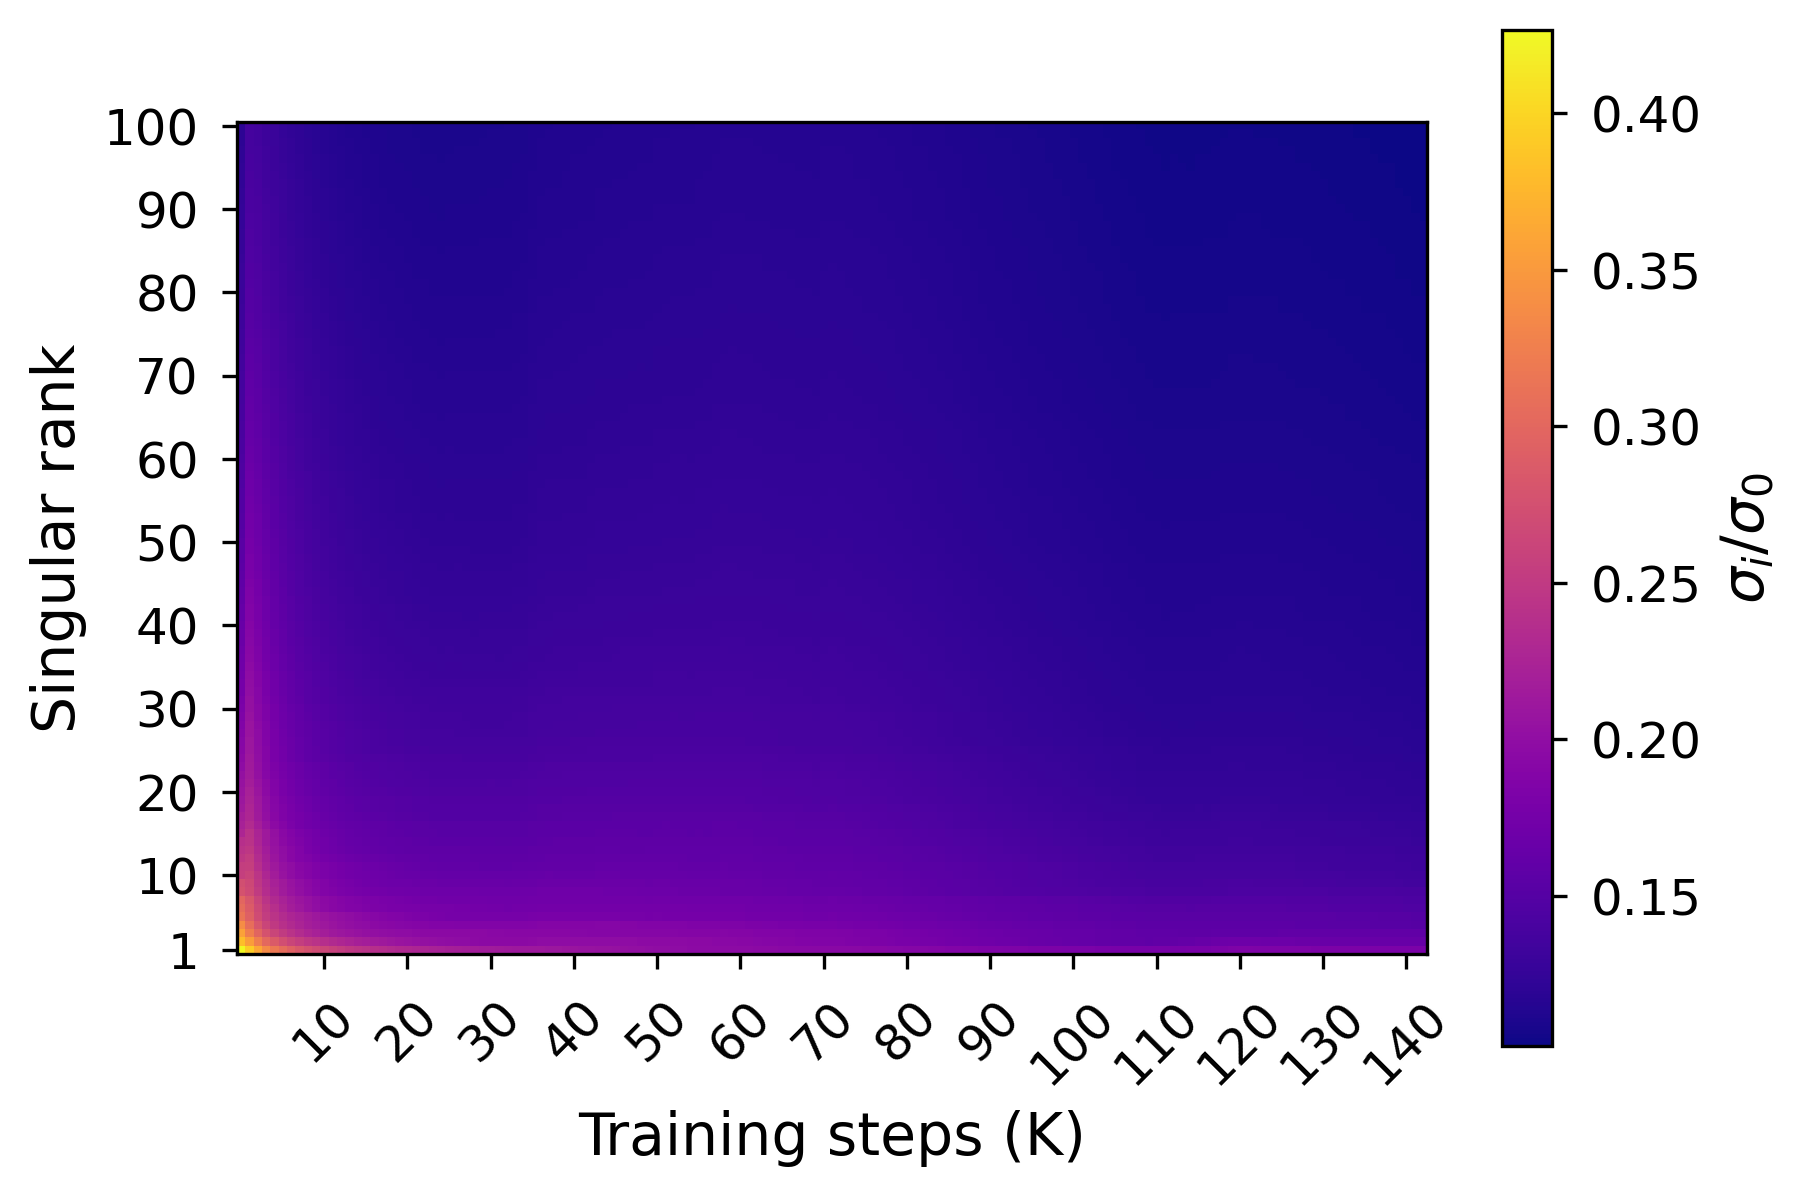
\includegraphics[width=\linewidth]{sources/part_1/softmax_bottleneck/imgs/sv_map_410m.png}
         \caption{410M}
         \label{fig:sv_410M}
    \end{subfigure}
    \caption{Evolution of the singular value distributions of the LM heads of Pythia models during training, normalized by the maximum singular value.}
    \label{fig:sv_evolve}
\end{figure}

\Cref{fig:sv_evolve} sheds light on a specific pattern of spectral saturation, roughly co-occurring with the performance saturation phenomenon. It shows that the singular value distribution progressively flattens during training, and nearly reaches uniformity before abruptly evolving towards a spiked distribution with a high maximal singular value, relatively to the other ones.

\begin{figure}[ht]
\centering
    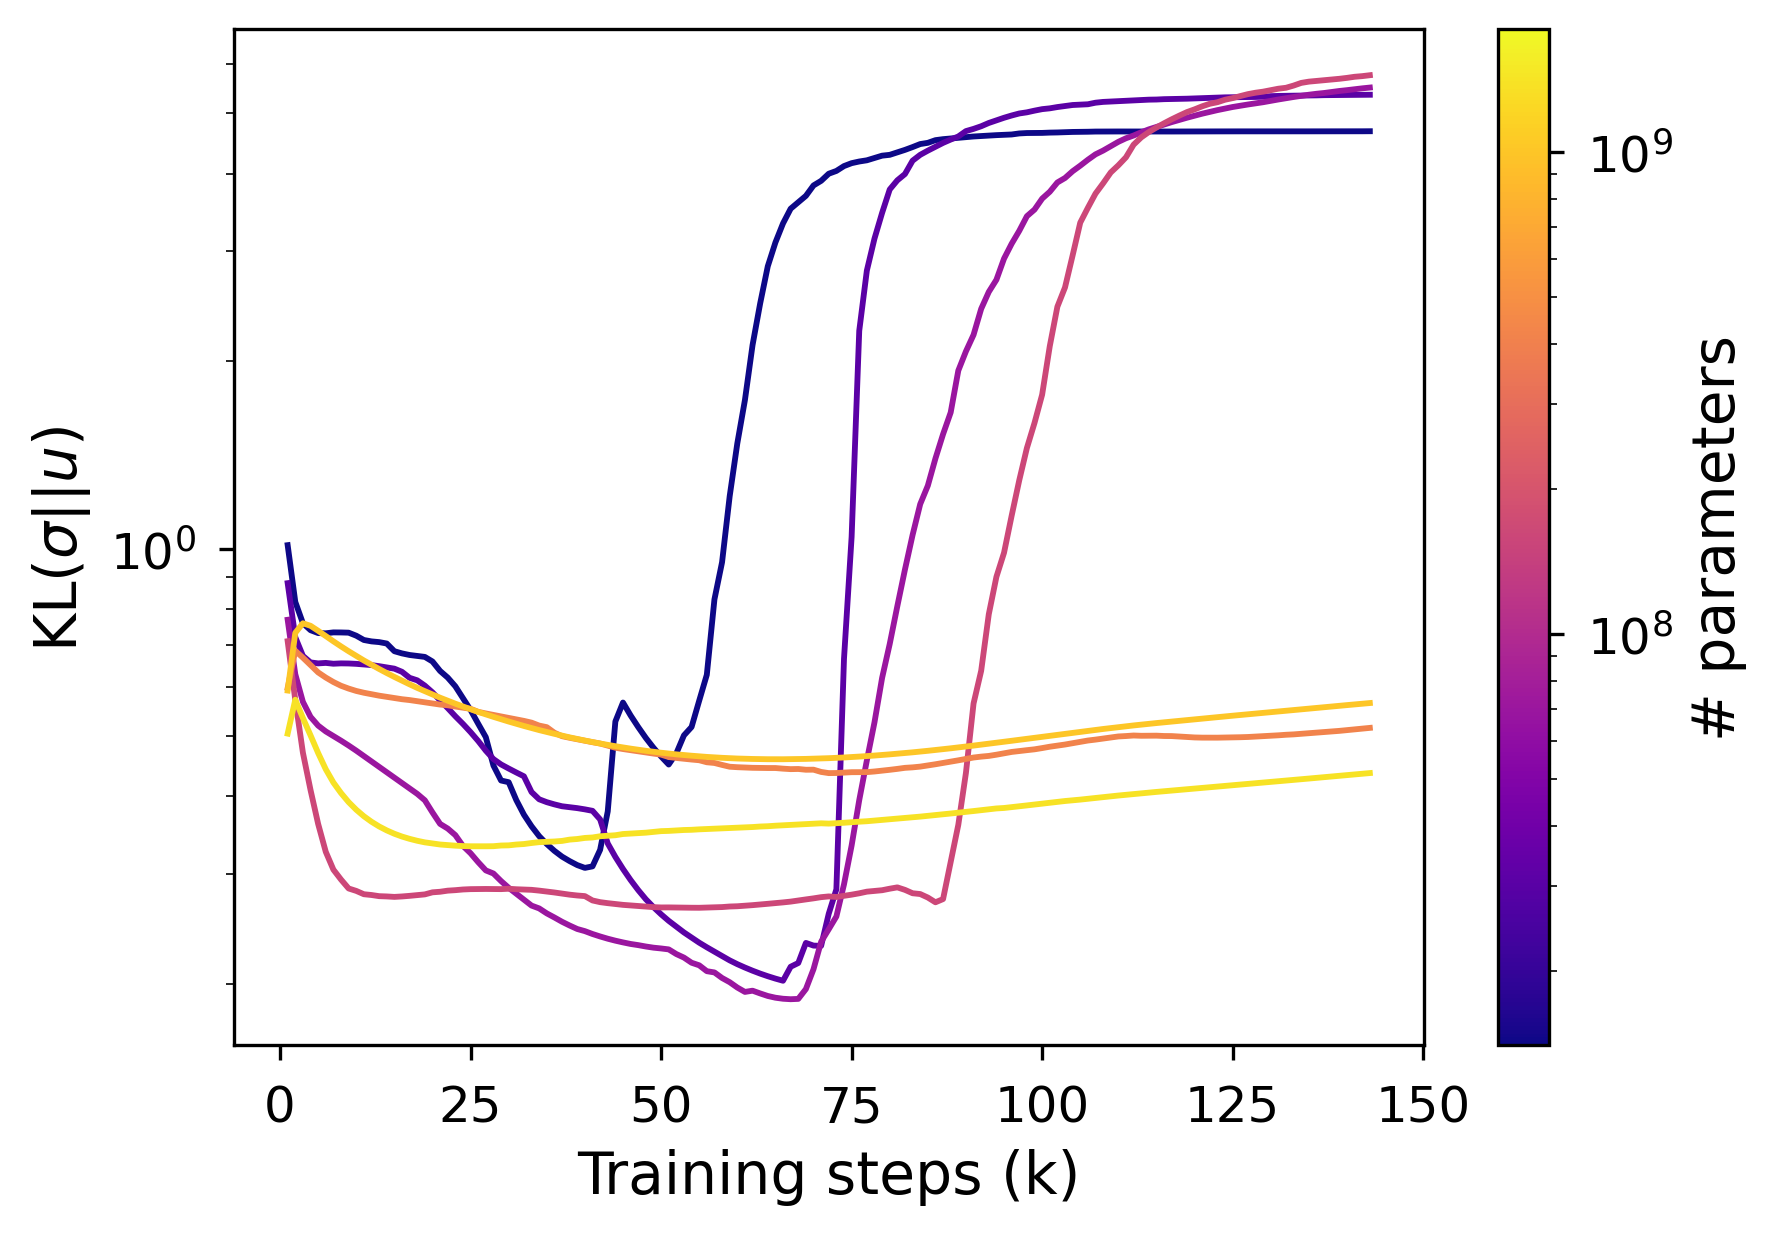
\includegraphics[width=0.6\textwidth]{sources/part_1/softmax_bottleneck/imgs/kullback_uni.png}
    \caption{Training dynamics of the singular entropy, for different Pythia models.}

    \label{fig:kl_div}
\end{figure}

In order to quantify this behavior more accurately, we use a \textit{singular entropy metric}, computed as the Kullback-Leibler divergence between the normalized singular value distribution and the uniform distribution.

\Cref{fig:kl_div} shows that singular distributions evolve differently for models using less than 410M parameters than for the larger ones. The heads of small models see their singular value distributions become increasingly uniform, up to a point where they degenerate abruptly, which again correlates with the LM performance drop. The singular value distributions of larger models tend to be more stable, and do not display clear monotonic patterns throughout training.

\section{The Softmax Bottleneck \& Language Dimensionality}
\subsection{Inherent Dimensionality of Natural Language}
\label{sec:inherent_dim}
% In practice, we can neither access $W^*$ nor $\phi^*$. However, we propose to use proxies for both in order to estimate the magnitude of the dimensionality of natural language in terms of singular spectrum.
Intuitively, the saturation of the singular values distribution observed only for smaller models in \Cref{sub:saturation} questions the dimensionalities involved in the optimization of the LM head. In this section, we propose to empirically measure a critical value for the rank of the LM head, and to estimate the dimensionality of the contextual probability distribution the head's outputs are supposed to match.

In order to empirically measure the effect of the rank of the linear head, we propose to train rank-constrained heads on pretrained contextual representations from highly-parameterized language models. In order to control the maximum rank $r$, we consider heads of the form $W = AB \in \mathbb{R}^{V \times d_m}$, where the coefficients of $A \in \mathbb{R}^{V \times r}$ and $B \in \mathbb{R}^{r \times d_m}$ are drawn from $\mathcal{N}(0, 1)$ ($d_m$ being the hidden dimension of the model). The rank of such $W$ matrices is limited by the parameter $r \in [1, d_m]$, which we sweep over a wide range of values.

We freeze the language models and train the rank-constrained heads on their output representations on roughly 150M tokens, while adjusting the learning rate to the trainable parameter count.

More precisely, we freeze the pretrained weights in the Transformer layers, and we train each rank-constrained head (i.e. in the form $W=AB$ with $r$ as the inner dimension of the matrix product) for various values of $r$ on 150M tokens sampled from The Pile using 4 V100 GPUs for the Pythia models and 4 A100 GPUs for Llama-7B. We use the hyperparameters from \citet{biderman2023pythia}, except for the batch size which we set to 256 as it fits our hardware setup better. As the trainable parameter count evolves with $r$, we search for the best-performing learning rates among values ranging from $1\cdot 10^{-3}$ to $5\cdot 10^{-2}$.

We report the chosen learning rates in \Cref{fig:lr_choices}.

\begin{figure}[ht]
\centering
    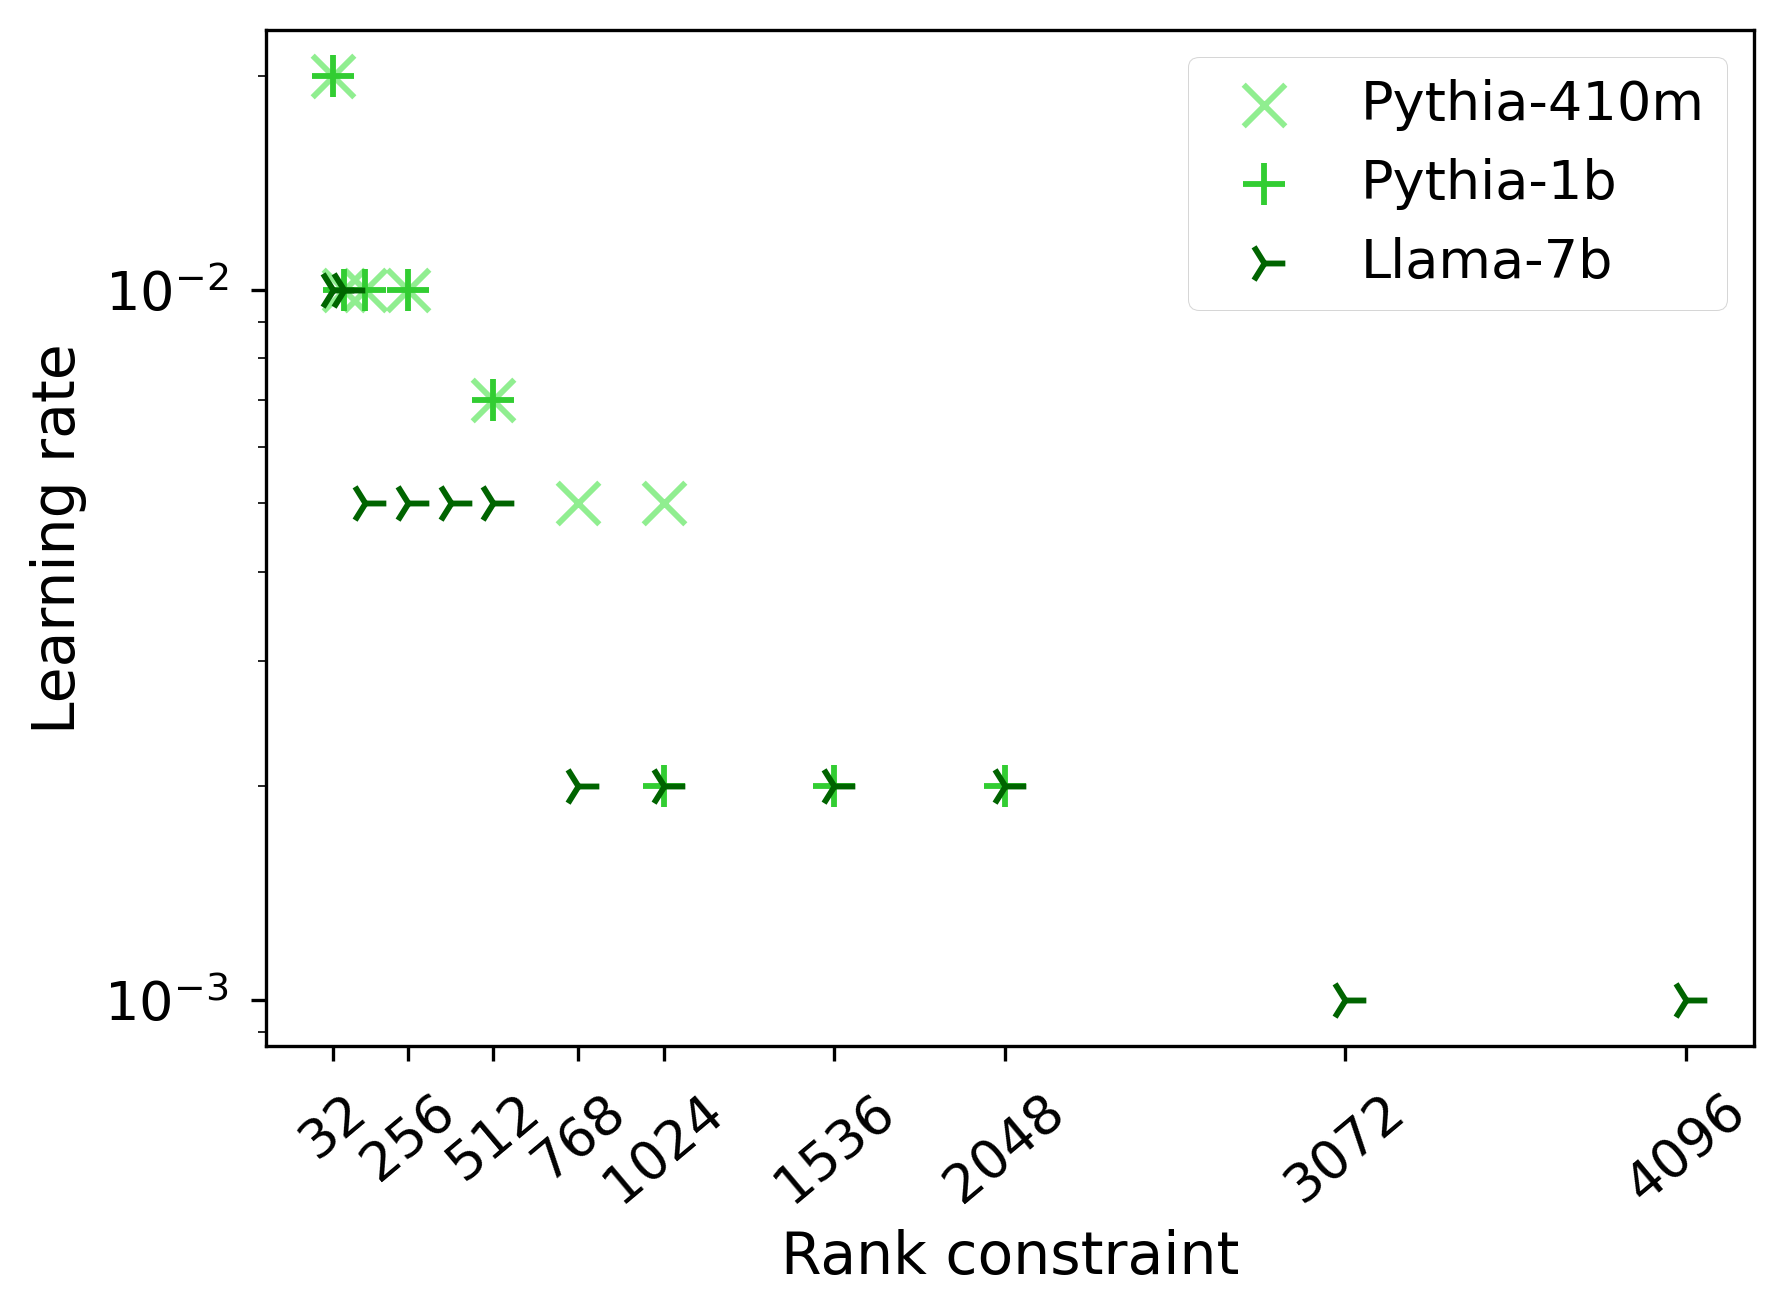
\includegraphics[width=0.6\linewidth]{sources/part_1/softmax_bottleneck/imgs/lr_final.png}
    \caption{Chosen peak learning rates used for the rank-constrained head experiments for each model.}
    \label{fig:lr_choices}
\end{figure}


\begin{figure}[ht]
\centering
    \begin{subfigure}{0.41\columnwidth}
         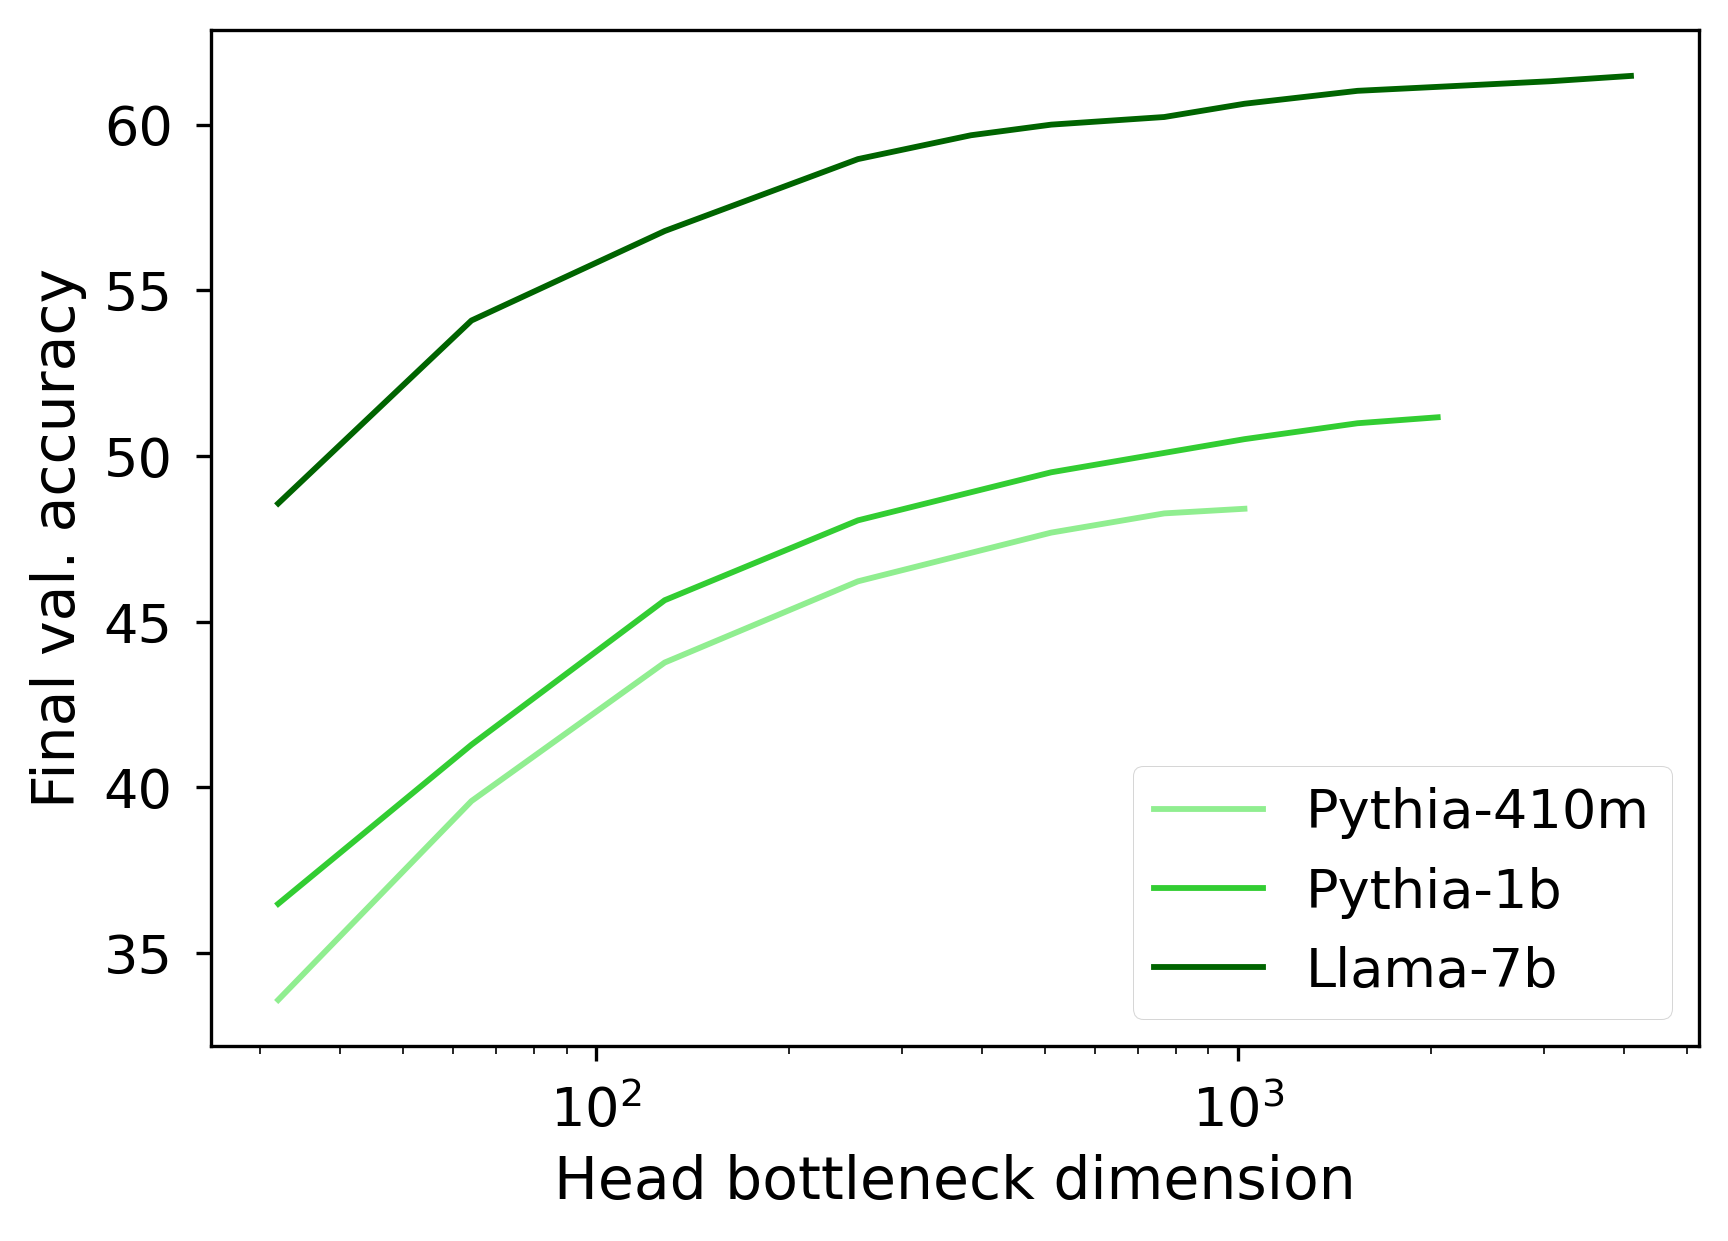
\includegraphics[width=\linewidth]{sources/part_1/softmax_bottleneck/imgs/llama_bottleneck_acc.png}
         \caption{Accuracy}
         \label{fig:bottleneck_acc}
    \end{subfigure}
    \begin{subfigure}{0.42\columnwidth}
         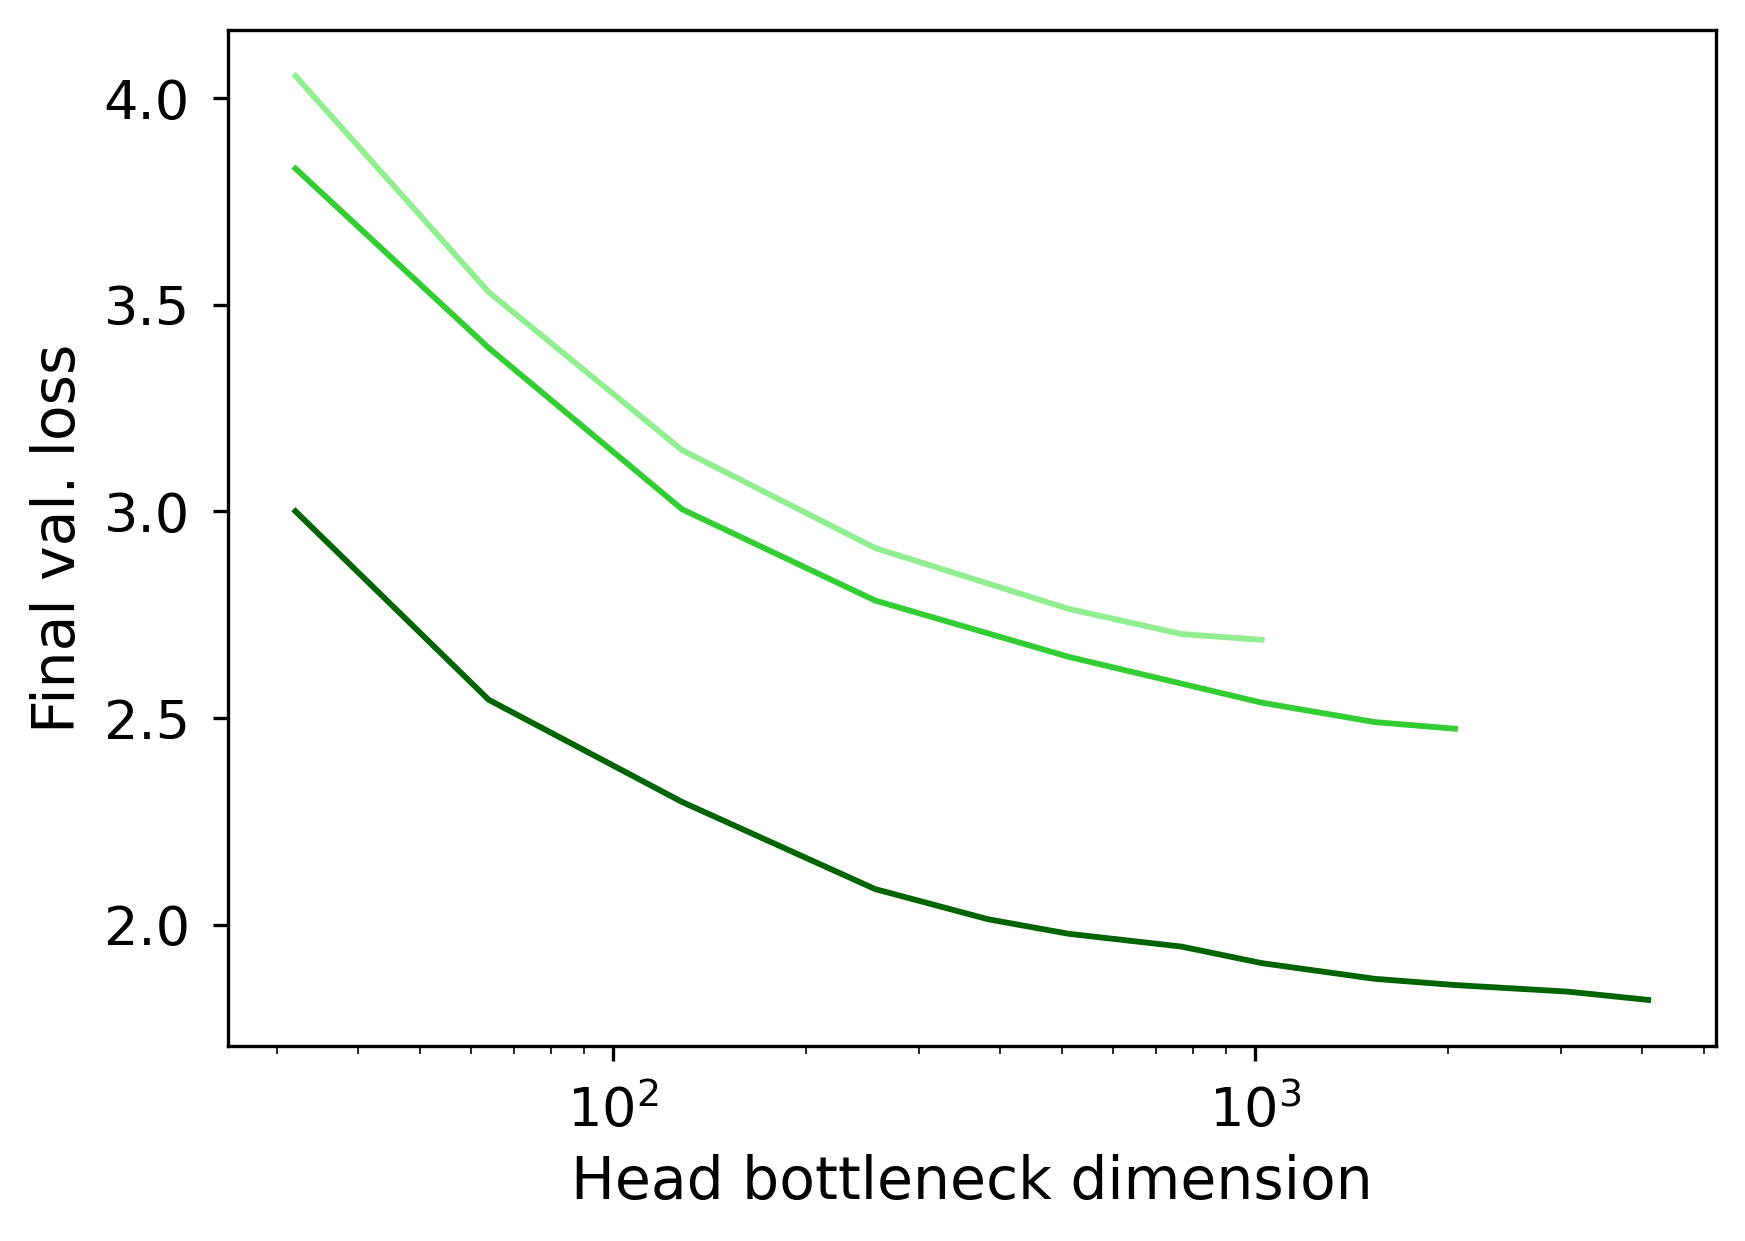
\includegraphics[width=\linewidth]{sources/part_1/softmax_bottleneck/imgs/llama_bottleneck_loss.png}
         \caption{Cross-entropy}
         \label{fig:bottleneck_ce}
    \end{subfigure}
    \caption{Performance of several models as the bottleneck dimension of the head increases.}
    \label{fig:perf_bottleneck}
\end{figure}
In \Cref{fig:perf_bottleneck}, we observe that perplexity starts to noticeably decrease when the rank of the language modeling head $W$ is roughly inferior to 1000, \textit{regardless of the model size}. This hints that the head is not a major performance bottleneck for models with greater hidden dimensions, but that it may hurt performance for models with smaller ones independently of the quality of the output representations.

Another interesting factor to estimate is the dimensionality inherent to the data itself. To avoid possible effects related to specific inductive biases, we train naive 5-gram language models on several datasets of varying coverage (IMDb \citep{imdb}, Wikitext \citep{wikitext}, and The Pile \citep{gao2020pile}), using two tokenizers of varying vocabulary sizes (30k tokens for Llama-2 and 50k tokens for Pythia). Given $C$ observed 5-grams, we consider the matrices $W \in \mathbb{R}^{C \times V}$ where each row is a probability distribution over possible tokens in a given 4-token context, and compute their singular value distributions, as in \citet{ngram_svd}. In \Cref{fig:w_error}, we report \textit{$W$\!-error}, the minimal approximation error on $W$ for a matrix of rank $d$ as predicted by the Eckart-Young-Mirsky theorem (see \Cref{eym}), normalized by the Frobenius norm of $W$:
$$
W\text{-error}(d) = \frac{||\sigma_{d+1:}||_2}{||W||_F}
$$
\begin{figure}[ht]
\centering
    \begin{subfigure}{0.415\columnwidth}
         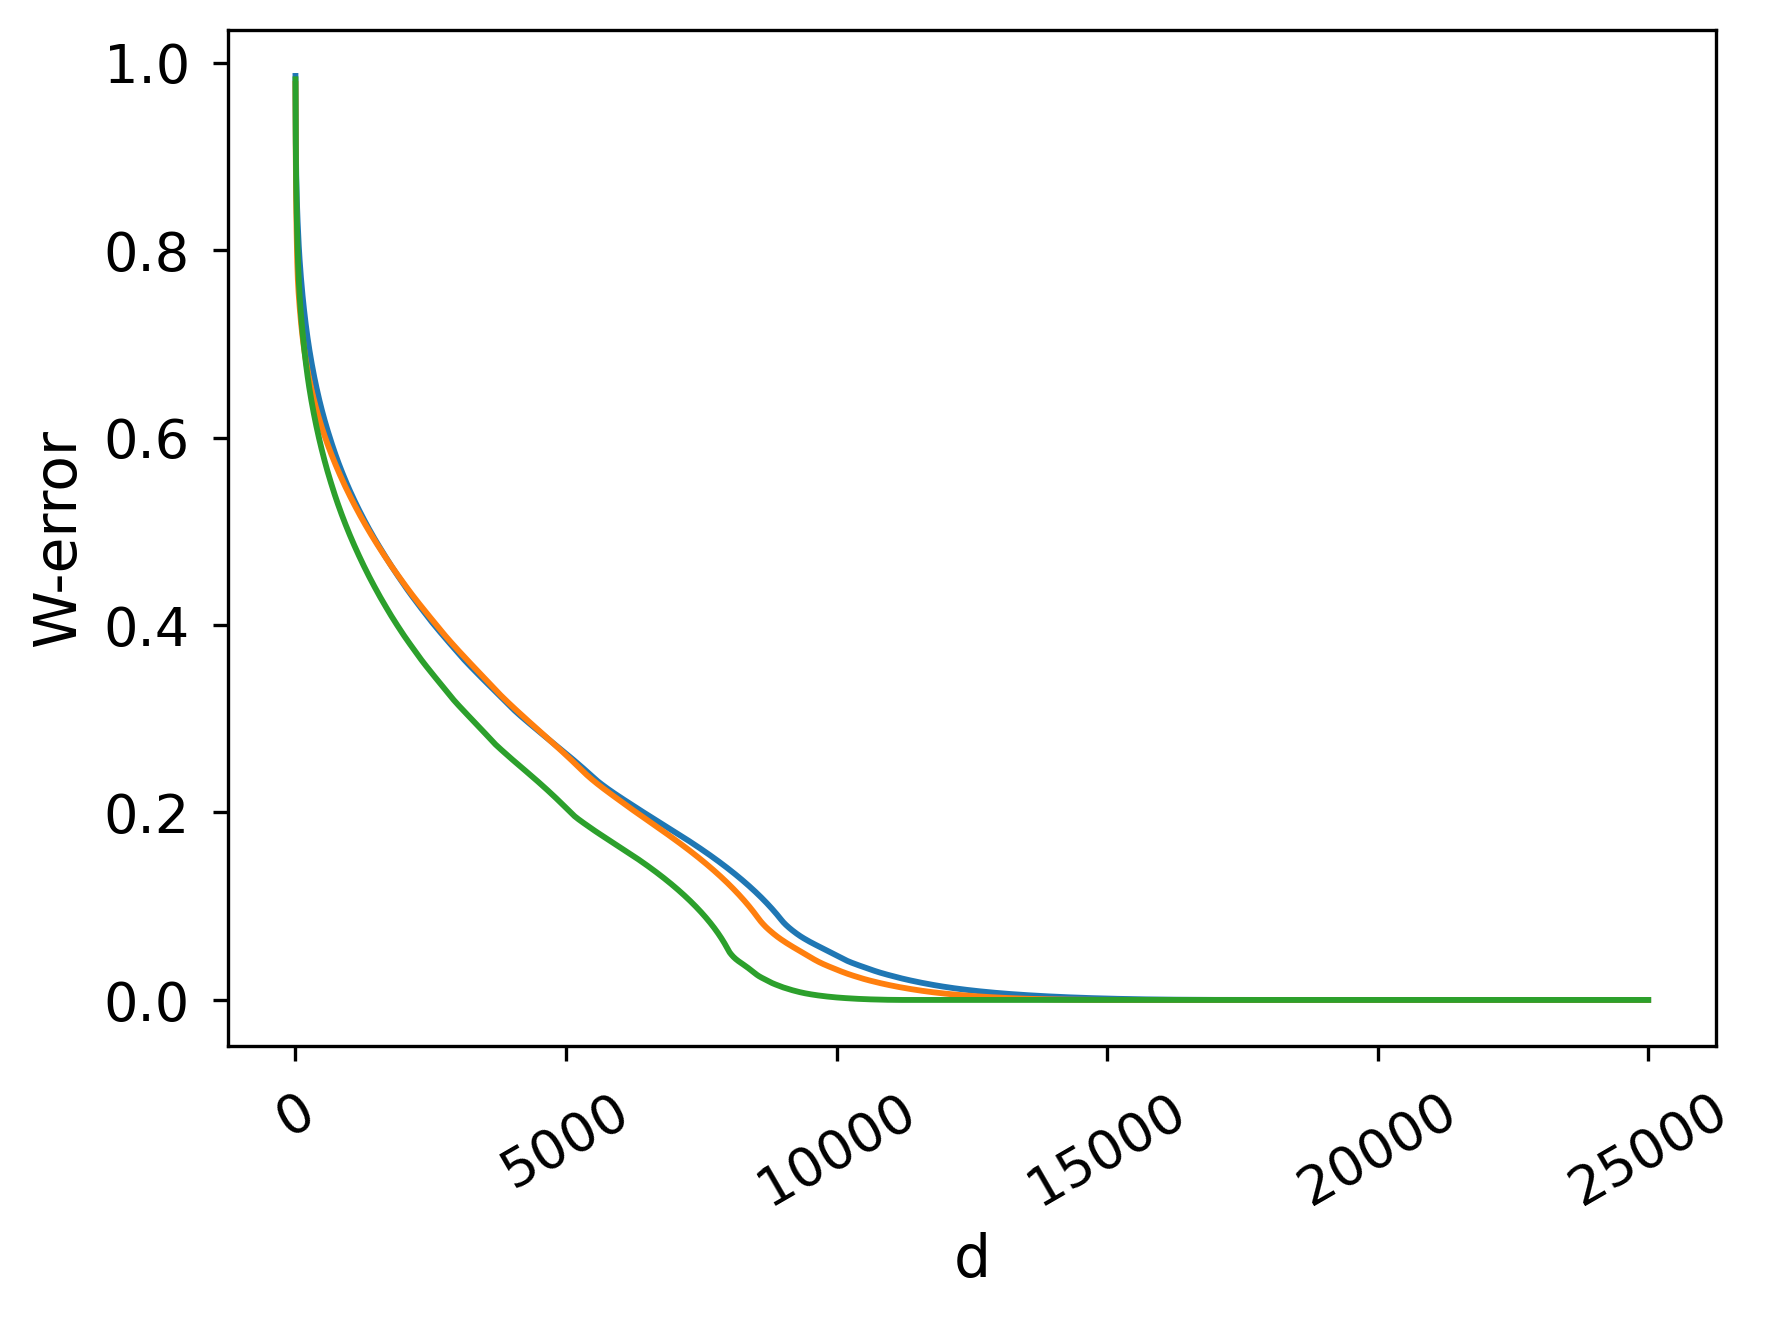
\includegraphics[width=\linewidth]{sources/part_1/softmax_bottleneck/imgs/llama_sv_4gram.png}
         \caption{Llama-2 tokenizer}
         \label{fig:llama}
    \end{subfigure}
    \begin{subfigure}{0.4\columnwidth}
         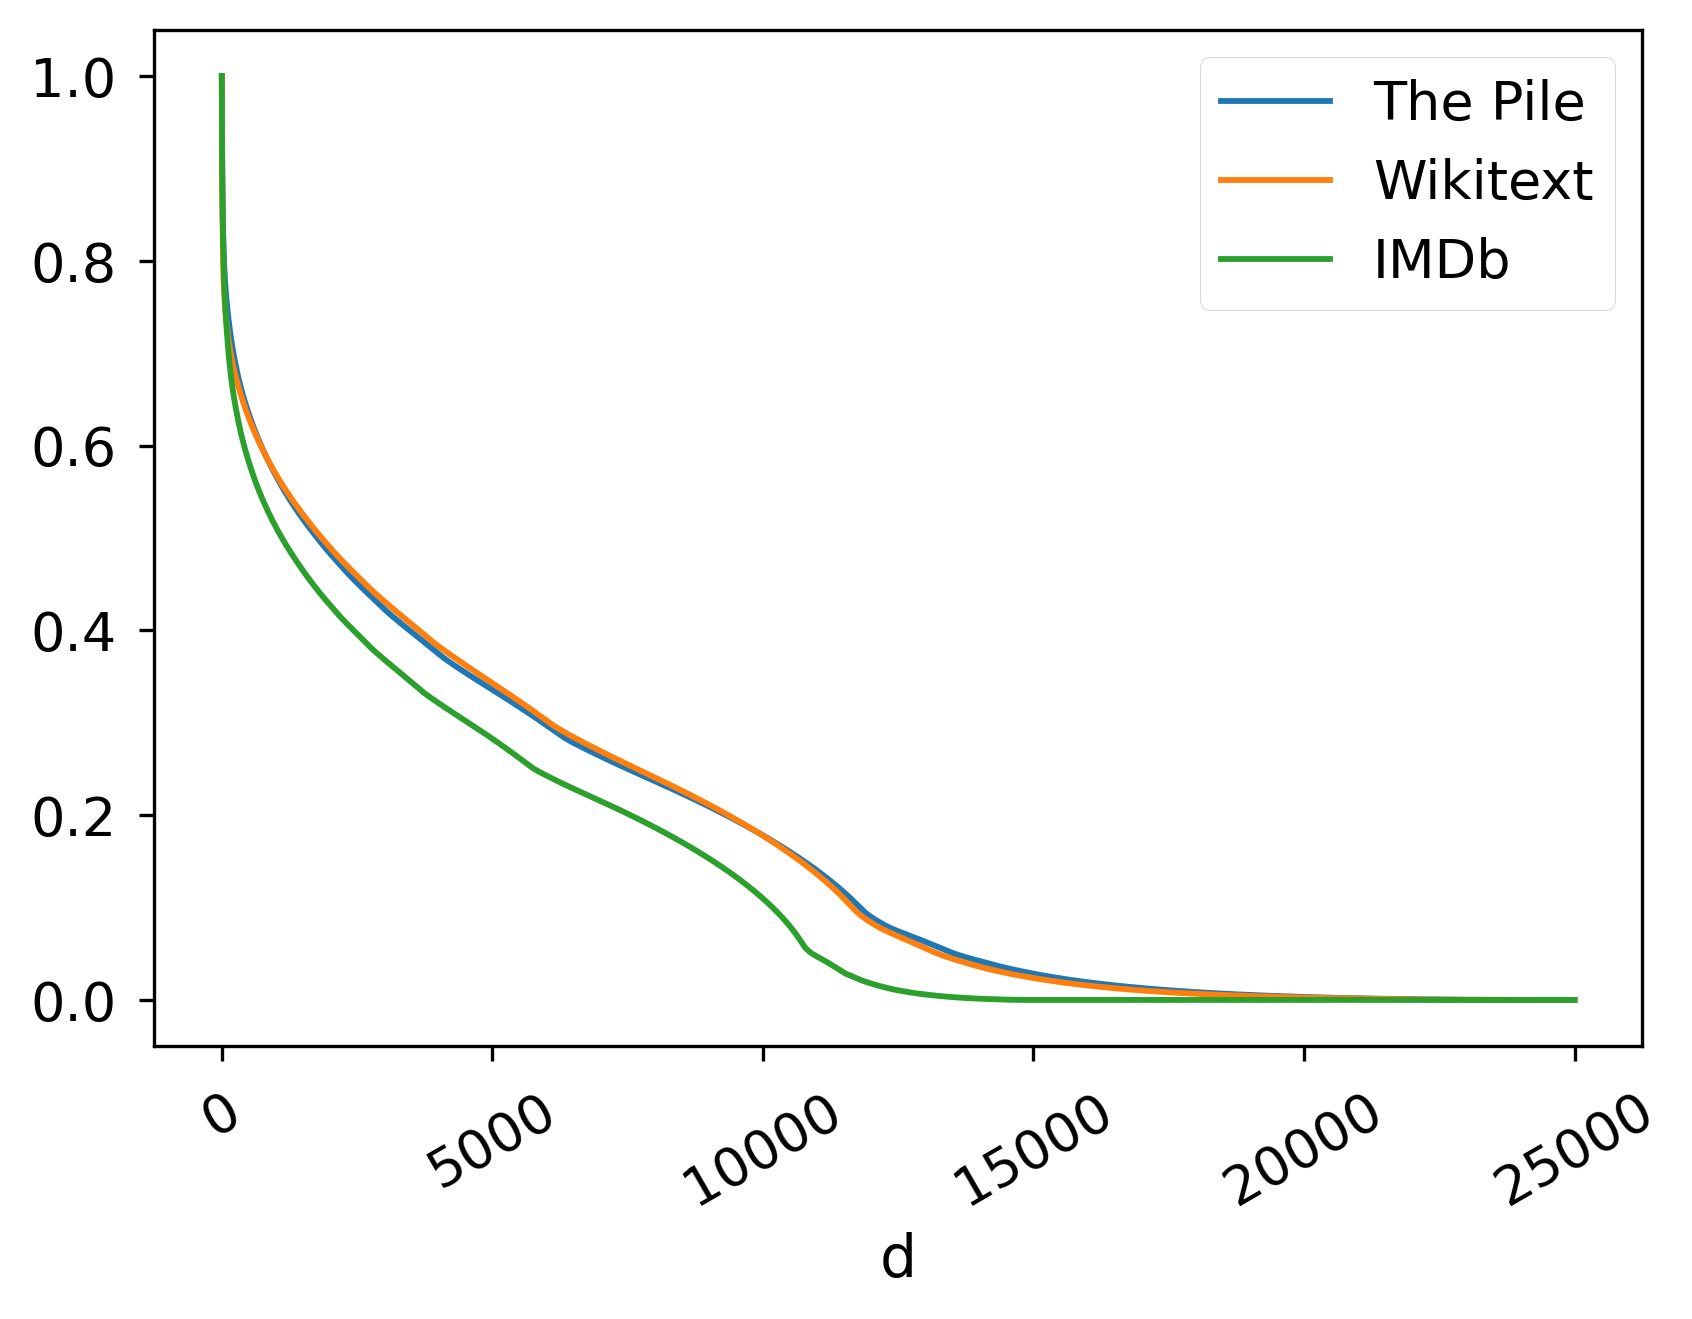
\includegraphics[width=\linewidth]{sources/part_1/softmax_bottleneck/imgs/pythia_sv_4gram.png}
         \caption{Pythia tokenizer}
         \label{fig:pythia}
    \end{subfigure}
    \caption{$W$\!-error as $d_m$ increases, for different tokenizers and datasets. We observe that while W-error can be halved using 1000 or 2000 dimensions, it only becomes negligible after 10,000-15,000 dimensions.}
    \label{fig:w_error}
\end{figure}

We find that the estimated rank of $W$ is non-negligible with respect to the usual magnitude of hidden dimensions. In the next section, we analyze the connection between the dimensionality of an ideal linear language modeling head and performance from a theoretical perspective.


\subsection{A Theoretical Bottleneck}
In this section, we aim at identifying a formal link between the inherent dimensionality of the contextual distribution and the performance bottleneck that can be attributed to the lower dimensionality of the output representations of a language model. To that end, we conceptualize a language modeling head optimized on \textit{ideal} contextual representations, and we explore the relationship between its spectral properties and the performance gap induced when training a low-rank head on the same representations.  

% Let's consider a set $\mathcal{T}$ of sequences $(y_i)_{i \in [1, |y|]}$ of elements taken from a vocabulary of size $V$, representing the pretraining data. We consider a function $\phi^*_D$ that \textit{perfectly} (e.g. in a bijective way) represents a given context $y_{< i}$ as a single real vector of \textit{sufficiently} high dimension $D \in \mathbb{N}^* \cup \{+\infty\}$. As we do not focus on $\phi^*_D$, we can simplify the notations by introducing the contextual representations $x^*_i = \phi^*_D(y_{< i})$. 

Let's consider a set $\mathcal{T}$ of sequences $(\mathbf{w}^i)_{i \in [1, |\mathcal{T}|]}$ of elements taken from a vocabulary of size $V$, representing the pretraining data. We consider a function $\phi^*$ that \textit{perfectly} (e.g. in a bijective way) represents a given context $\mathbf{w}^i_{<t}$ as a single real vector of \textit{infinite} dimension. As we do not focus on $\phi^*$, we can simplify the notations by introducing the contextual representations $h^*_{i,t} = f^*(\mathbf{w}^i_{<t})$. 

The task of the linear language modeling head can be formalized as an optimization problem on the matrix $W$:
\begin{equation}
W^* = \argmin_{W \in \mathbb{R}^{V \times \infty}} \sum_{i=1}^{|\mathcal{T}|} \sum_{t=1}^{|\mathbf{w}^i|} \mathcal{L}(W, h^*_{i,t}, w^i_t)
\label{eq:unconstrained}
\end{equation}

where $\mathcal{L}$ is the cross-entropy objective defined using the softmax function $\sigma$ as:
$$
\mathcal{L}(W, h, w) = - \log (\sigma(Wh)_{w})
$$

% Without loss of generality, we choose $D$ to be large enough so that setting up this problem using $D+1$ would not lead to a better performance in \autoref{eq:unconstrained}.

In practice, a neural language model $f_\theta$ produces contextual representations $h_{i,t} = f_\theta(\mathbf{w}^i_{<t})$ of dimension $d_m \in \mathbb{N}^*$. The linear language modeling head $W_\theta \in \mathbb{R}^{V \times d_m}$ is trained concurrently with $f_\theta$ with the same objective as in \autoref{eq:unconstrained}.

We focus on the maximal expressiveness of a lower-dimensional head: when provided with \textit{perfect} contextual representations $h^*_{i,t}$, what is the maximal performance level of a linear language modeling head of maximal rank $d$? This question can be put in mathematical terms:

\begin{equation}
W_d^* = \argmin_{W \in \mathbb{R}^{V \times \infty}} \sum_{i=1}^{|\mathcal{T}|} \sum_{t=1}^{|\mathbf{w}^i|} \mathcal{L}(W, h^*_{i,t}, w^i_t) \text{ s.t. } \rank(W) \leq d
\label{eq:constrained}
\end{equation}

% MADE THINGS COMPLICATED with x*:
% \Cref{best_on_all} shows that any alternative to the $W^*$ matrix, including a low-rank approximation, cannot improve performance in any context.


% \begin{lemma}
% \label[lemma]{best_on_all}{(proof in \Cref{app:best_on_all})}
% By construction of $W^*$, for all $W \in \mathbb{R}^{V \times \infty}$, $y \in \mathcal{T}$ and $x^* = \phi^*(y)$, we have:
% $$
% \mathcal{L}(W, x^*, y) \geq \mathcal{L}(W^*, x^*, y)
% $$
% \end{lemma}


\Cref{linear_rel} shows that by approaching $W^*$ directly, we can asymptotically expect to close the performance gap.

\begin{lemma}
\label[lemma]{linear_rel}
Let's consider $W \in \mathbb{R}^{V \times \infty}, M \in \mathcal{H}^{V \times \infty}$ the matrix unit sphere for the Frobenius norm $||\cdot||_F$, and $\varepsilon \in \mathbb{R}^*_+$ such that $W = W^* + \varepsilon M$ . When $\epsilon \rightarrow 0$, for all $h \in \mathbb{R}^d$ and $w \in [1, V]$:
$$
|\mathcal{L}(W, h, w) - \mathcal{L}(W^*, h, w)|  = O(\varepsilon)
$$
\end{lemma}
\begin{proof}
     The proof is mainly based on calculations and limited development:
     \begin{align*}
     & |\mathcal{L}(W, h, w) - \mathcal{L}(W^*, h, w)| \\
     & =
     \left| -\log \frac{\exp((Wh)_w)}{\sum_{j \in V} \exp((Wh)_{w})} + \log\frac{\exp((W^*h)_{w})}{\sum_{j \in V} \exp((W^*h)_w)}\right| \\
     & =  \left|-(\varepsilon Mh)_{w} + \log \frac{\sum_{j \in V} \exp((W^*h)_{j}) \exp((\varepsilon Mh)_{j})}{\sum_{j \in V} \exp((W^*h)_{j})}\right| \\
     & = \left| - \varepsilon (M h)_{w} + \log\left( 1 + \frac{\sum_{j \in V} \varepsilon \exp((Mh)_{j})}{\sum_{j \in V} \exp((W^*h)_{j})} + o(\varepsilon) \right) \right| \\
     & = \left| -\varepsilon (M h)_{w} + \varepsilon  \frac{\sum_{j \in V} \exp((Mh)_{j})}{\sum_{j \in V} \exp((W^*h)_{j})} \right| + o(\varepsilon) \\
     & = \varepsilon \left| - (M h)_{w} + \frac{\sum_{j \in V} \exp((Mh)_{j})}{\sum_{j \in V} \exp((W^*h)_{j})} \right| + o(\varepsilon)
     \end{align*}
     
     The continuous function $M \longrightarrow \left| - (M h)_{w} + \frac{\sum_{j \in V} \exp((Mh)_{j})}{\sum_{j \in V} \exp((W^*h)_{j})} \right|$ is bounded on the compact matrix unit sphere (i.e. where $||M||_F = 1$), which ends the proof.
     
     \textbf{Remark : }This result could also be proven using a differentiability argument, but we prefer to display a more precise relation between the loss gap and the error on the $W$ matrix approximation, stressing out its quasi-linear nature. This formulation will hopefully pave the way for further exploration of this relation in future works.
     
\end{proof}

% \begin{lemma}
% \label[lemma]{linear_rel}{(proof in \Cref{app:linear_rel})}
% Let's consider $W \in \mathbb{R}^{V \times \infty}, M \in \mathcal{H}^{V \times \infty}$ the matrix unit sphere for the Frobenius norm $||\cdot||_F$, and $\varepsilon \in \mathbb{R}^*_+$ such that $W = W^* + \varepsilon M$ . When $\epsilon \rightarrow 0$:
% $$
% |\mathcal{L}(W, x^*_i, y_i) - \mathcal{L}(W^*, x^*_i, y_i)|  = K_{W^*, x^*, y} \cdot \varepsilon + o(\varepsilon)
% $$
% \end{lemma}

Hence, our problem is linked to a low-rank matrix approximation \citep{low_rank}, which has direct connections with spectral theory. In our case, we can use the Eckart–Young–Mirsky theorem.

\begin{lemma}
\label[lemma]{eym}{(Eckart–Young–Mirsky theorem)}
Let's consider $(\sigma_i)$ the singular values of $W^*$ in decreasing order, and $\mathcal{M}_d$ the set of matrices in $\mathbb{R}^{V \times \infty}$ of rank $d < V = \rank(W^*)$. Then:
$$
\min_{W_d \in \mathcal{M}_d}||W_d - W^*||_F = \sqrt{\sum_{i=d+1}^{V} \sigma_i^2}
$$
\end{lemma}

Combining all of the above yields \Cref{main_thm}.
% Stronger but weaker
% \begin{lemma}
% \label[lemma]{linear_rel}{(proof in \Cref{app:linear_rel})}
% Let's consider $W \in \mathbb{R}^{D \times V}$, $M \in \mathcal{H}^{D \times V}$ the matrix unit sphere for the Frobenius norm $||\cdot||_F$, and $\epsilon \in \mathbb{R}^*_+$ such that $W = W^* + \epsilon M$ . When $\epsilon \rightarrow 0$, there is a constant $K_{W^*, x^*_i, M} \geq 0$ such that:
% $$
% |\mathcal{L}(W, x^*_i, y_i) - \mathcal{L}(W^*, x^*_i, y_i)| \geq \epsilon K_{W^*, x^*_i, M} + o(\epsilon)
% $$
% \end{lemma}

%From \Cref{linear_rel}, we know that minimizing $||W_d^* - W^*||_F$ also minimizes \autoref{eq:constrained}.%

\begin{theorem}
\label{main_thm}
Let's consider $(\sigma_i)$ the singular values of $W^*$ in decreasing order. Then, when $d \rightarrow V$, the loss gap induced by a $d$-dimensional bottleneck on the linear LM head follows:
$$
\sum_{i=1}^{|\mathcal{T}|} \sum_{t=1}^{|\mathbf{w}^i|} \mathcal{L}(W_d^*, h^*_{i,t}, w^i_t) - \mathcal{L}(W^*, h^*_{i,t}, w^i_t) = O\left(\sqrt{\sum_{i=d+1}^{V}\sigma_i^2}\right)$$
\end{theorem}
\begin{proof}
     Let us note $W_d$ the best approximation of $W^*$ of rank $d$ with respect to the Frobenius norm. By the triangle inequality, we have that:

\begin{equation}
\label{eq:approx}
\resizebox{\columnwidth}{!}{$\left|\sum_{i=1}^{|\mathcal{T}|} \sum_{t=1}^{|\mathbf{w}^i|} \mathcal{L}(W_d^*, h^*_{i,t}, w^i_t) - \mathcal{L}(W^*, h^*_{i,t}, w^i_t)\right| \leq \sum_{i=1}^{|\mathcal{T}|} \sum_{t=1}^{|\mathbf{w}^i|} \left|\mathcal{L}(W_d, h^*_{i,t}, w^i_t) - \mathcal{L}(W^*, h^*_{i,t}, w^i_t)\right|$}
\end{equation}


% We know from \Cref{best_on_all} that for all $y\in\mathcal{T}$ and $i \in [1, |y|]$:
% $$
% \mathcal{L}(W_d, x^*_i, y_i) - \mathcal{L}(W^*, x^*_i, y_i) \geq 0
% $$

The Eckart-Young-Mirsky theorem tells us that when $d \rightarrow V$, 
$$||W_d - W^*||_F = \sqrt{\sum_{i=d+1}^{V} \sigma_i^2} \rightarrow 0$$

By defining $\varepsilon = W_d - W^*$, we can apply \Cref{linear_rel} and show that:
$$
\left|\mathcal{L}(W_d, h^*_{i,t}, w^i_t) - \mathcal{L}(W^*, h^*_{i,t}, w^i_t)\right| = O(||W_d - W^*||_F) = O\left(\sqrt{\sum_{i=d+1}^{V} \sigma_i^2}\right)
$$

From \Cref{eq:approx}, we have that:
$$
\left|\sum_{i=1}^{|\mathcal{T}|} \sum_{t=1}^{|\mathbf{w}^i|} \mathcal{L}(W_d^*, h^*_{i,t}, w^i_t) - \mathcal{L}(W^*, h^*_{i,t}, w^i_t)\right| = O\left(\sqrt{\sum_{i=d+1}^{V} \sigma_i^2}\right)
$$

By definition of $W^*$ and $W_d^*$, we also have that:
$$
0 \leq \sum_{i=1}^{|\mathcal{T}|} \sum_{t=1}^{|\mathbf{w}^i|} \mathcal{L}(W_d^*, h^*_{i,t}, w^i_t) - \mathcal{L}(W^*, h^*_{i,t}, w^i_t)
$$
which ends the proof.

\paragraph{Remark} The bound used in \Cref{eq:approx} can be rather loose in practice. We can think of no particular reason why approaching $W^*$ directly should be the optimal way to minimize the loss on $\mathcal{T}$. Hence, the presented result should be taken carefully, and we leave the refinement of such an analysis for future work.

\end{proof}
These properties shed light on how the dimensionality of the ideal language modeling head impacts the performance when the LM head is low-rank. However, the relation obtained in \Cref{main_thm} is not particularly strong, as discussed in the proof.

In \Cref{fig:neg_res_thm}, we compare the results of the head bottleneck experiment of the Pythia-1B model in \Cref{sec:inherent_dim} to the $W$\!-error on the head of the same model as the bottleneck dimension $d$ evolves. It shows that the loss gap grows slowly with the $W$\!-error, implying that even when the allowed rank would lead to a poor approximation of $W$, the performance can still remain acceptable. We notice that the performance starts decreasing when the $W$\!-error outgrows 0.6.

\begin{figure}
\centering
    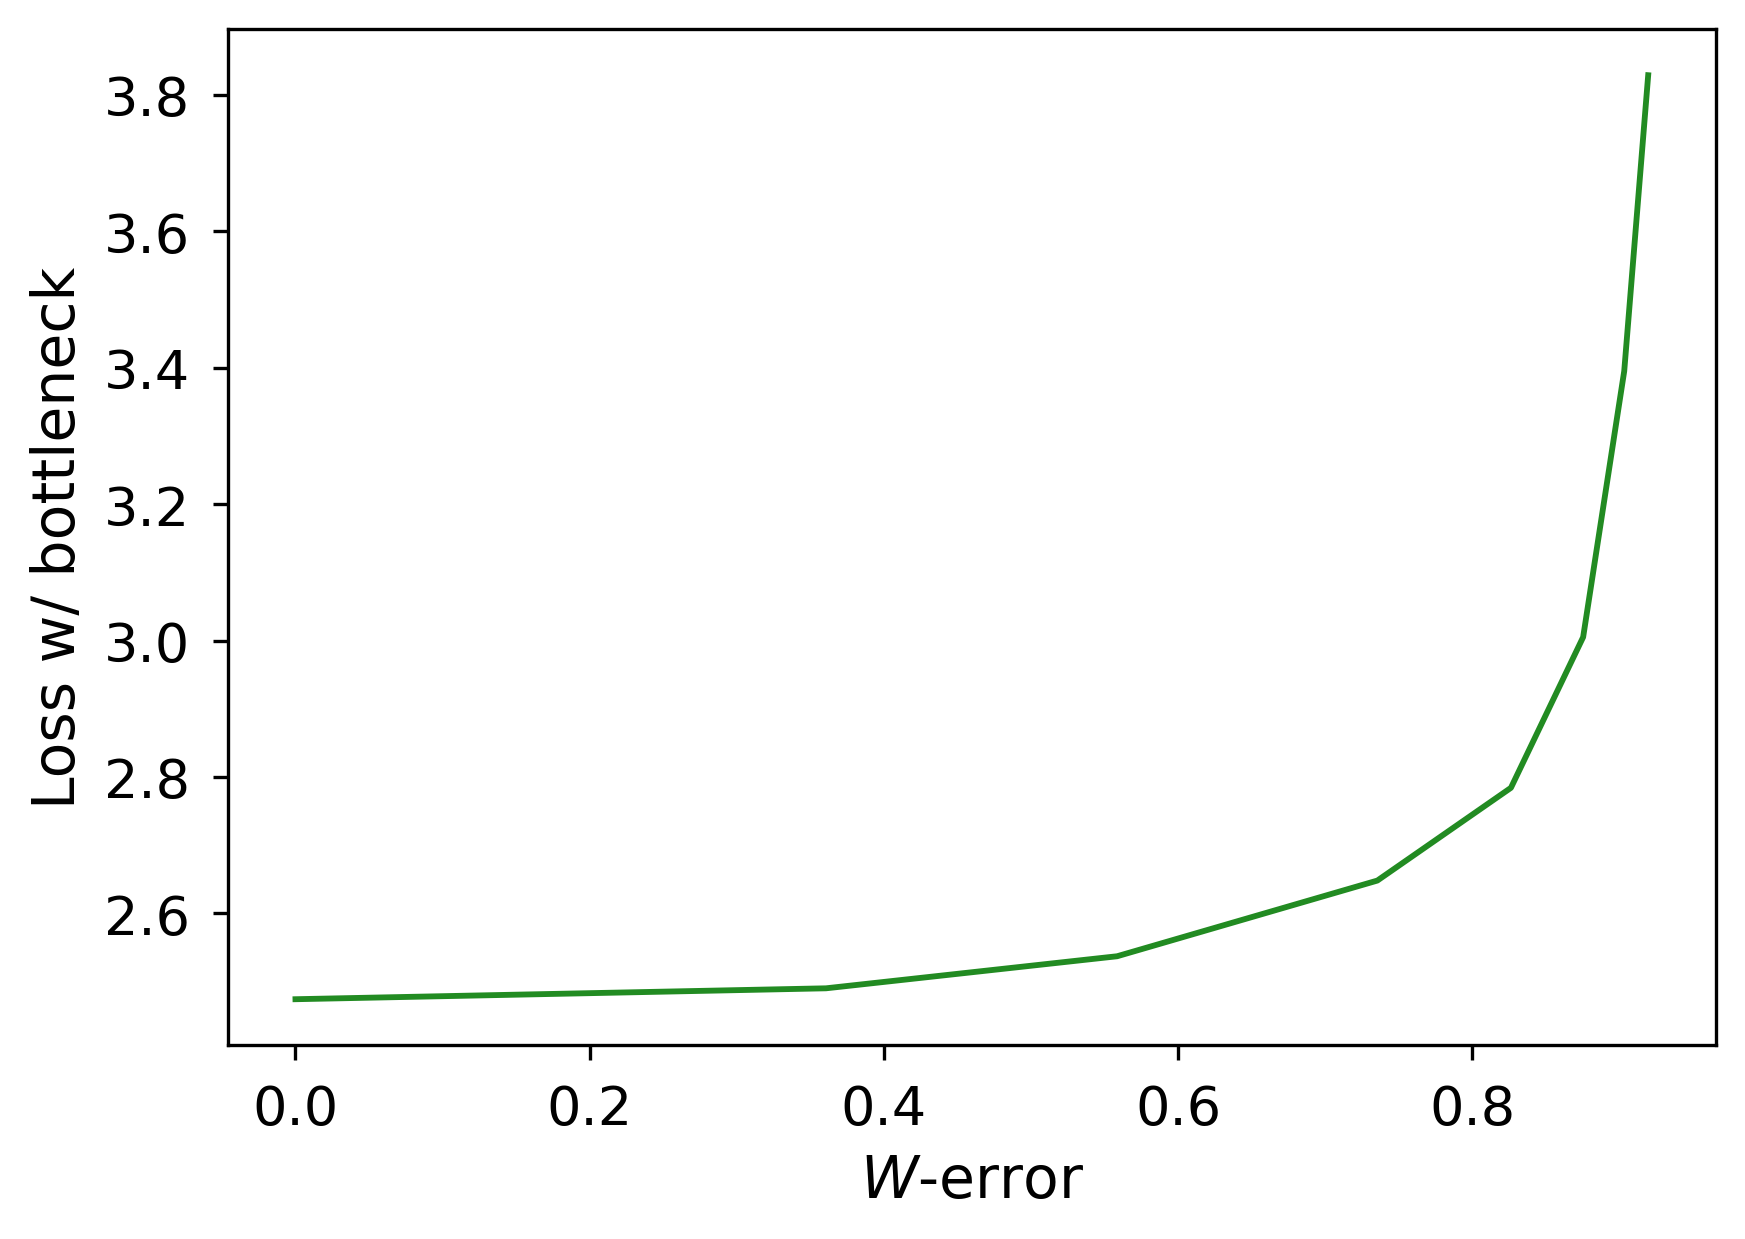
\includegraphics[width=0.6\textwidth]{sources/part_1/softmax_bottleneck/imgs/loss_v_werr.png}
    \caption{Final loss with trained rank-constrained heads (mimicking $W_d^*$), as a function of the theoretical $W$\!-error for rank $d$ on the head of the Pythia-1B model.}
    \label{fig:neg_res_thm}
\end{figure}

% \begin{figure}[ht]
% \centering
%     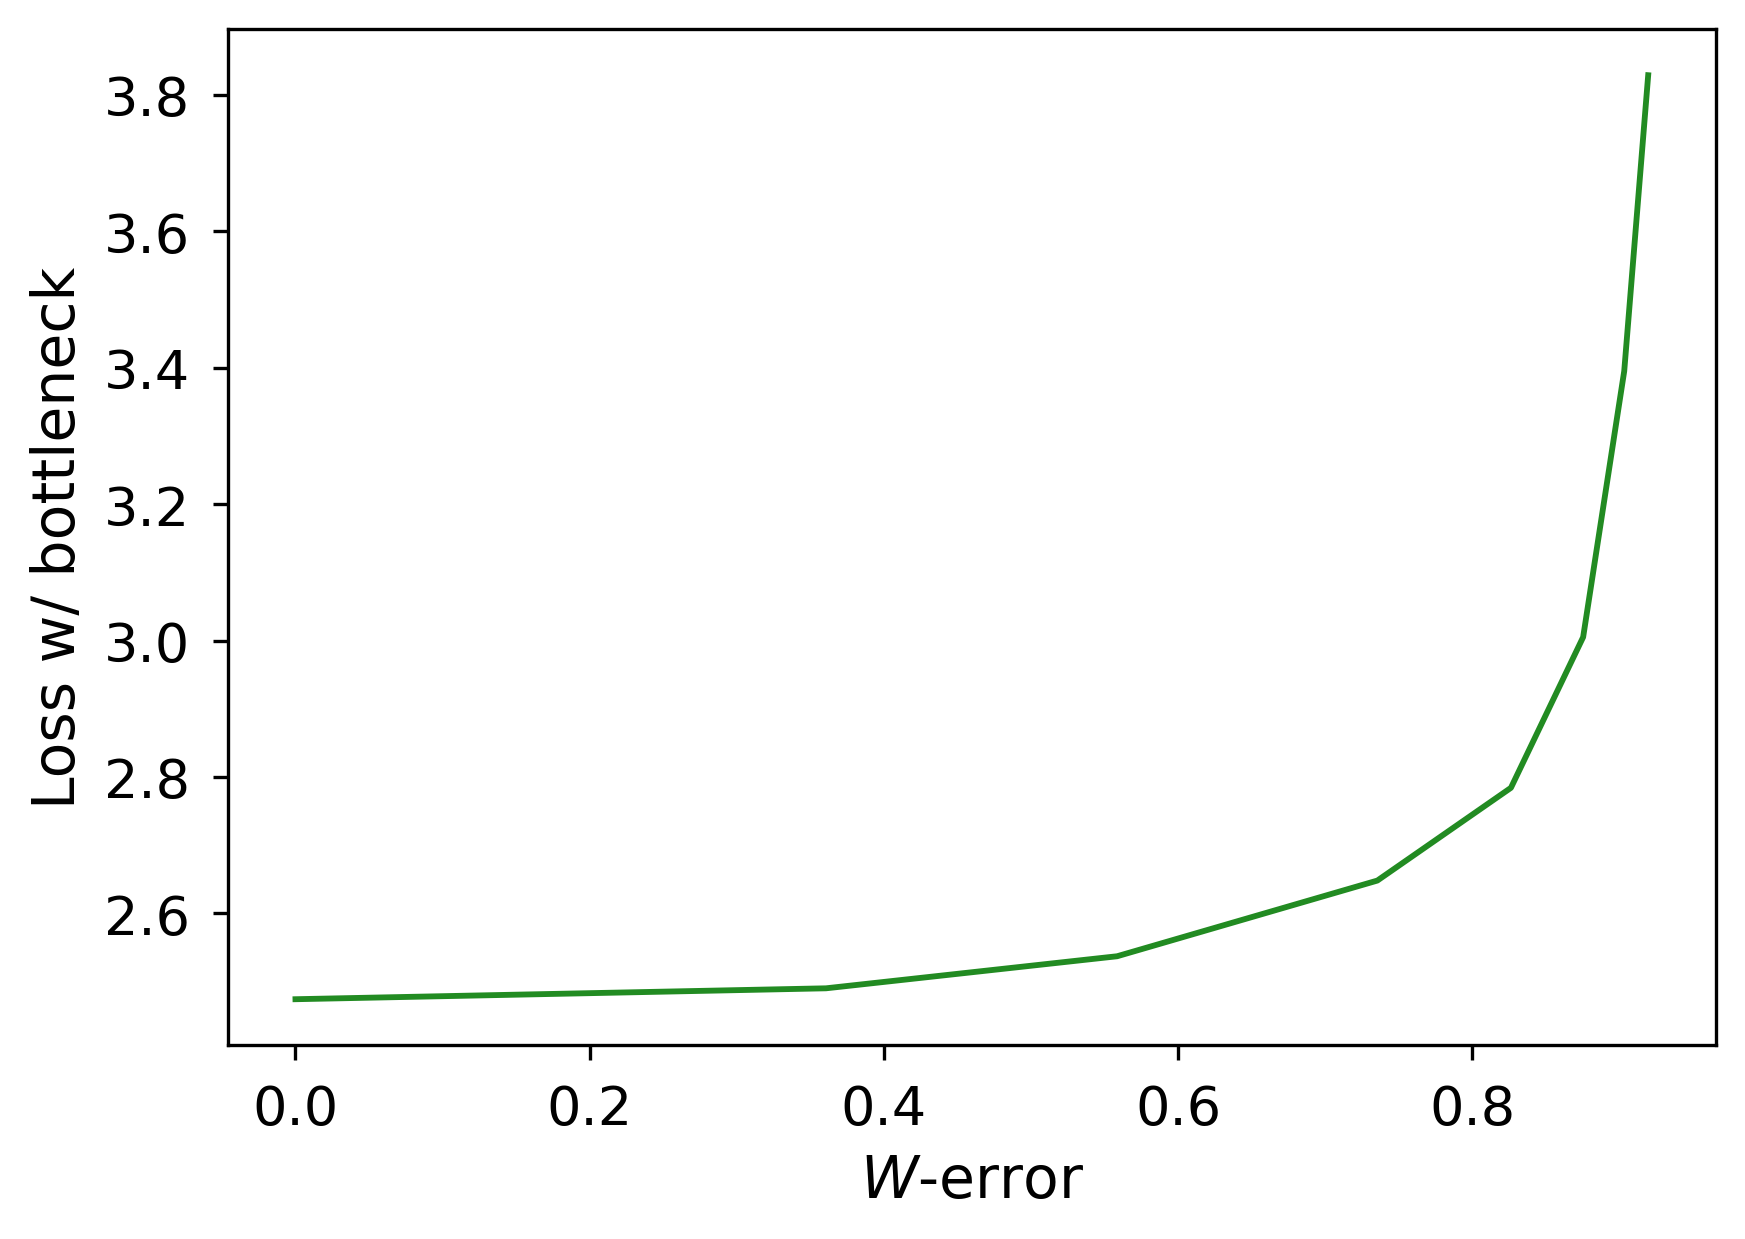
\includegraphics[width=0.4\linewidth]{sources/part_1/softmax_bottleneck/imgs/loss_v_werr.png}
%     \caption{Final loss with trained rank-constrained heads (mimicking $W_d^*$), as a function of the theoretical $W$\!-error for rank $d$ on the head of the Pythia-1B model.}
%     \label{fig:neg_res_thm}
% \end{figure}

% This is mostly due to the peculiar nature of the target distributions, which make a direct low-rank approximation to $W^*$ particularly suboptimal in terms of cross-entropy loss. 

% Moreover, contexts are far from uniformly distributed, which means that the optimal overall low-rank performance can be further optimized by focusing on the more frequent contexts. A better frame for this problem would be weighted low-rank approximation \citep{srebro2003weighted}; however, such an optimization problem does not have a closed form to the best of our knowledge. We leave exploration in this direction for future work.



% \subsection{The Role of Unigram Frequency}
% We have shown that the LM head of a small model tends to adopt a degenerated state in late training, which is correlated with the low performance of the resulting model. In this section, we propose to study this degenerated state at representation level, in order to understand what it implies for the model behavior and why it may lead to suboptimal performance.

% \textcolor{blue}{
% What will be here?
% \begin{itemize}
%     \item a figure showing how the norm of the average output representation increases in training, and how it aligns with frequency ($\sigma(W\bar{x}) \rightarrow f$)
%     \item conclusion: frequency becomes more important during training
%     \item empirical examples of high frequency terms appearing too often in generation after explosion vs. before
% \end{itemize}
% }
\section{Discussion}

% This paper provides insights on the performance bottleneck represented by linear language modeling heads, stressing out that the dimensionality of the target contextual distribution is poorly matched by language models that rely on small hidden dimensions.

One way to address the problem at hand could be to train shallow small language models, increasing hidden dimension at the expense of other hyperparameters, such as layer count or feed-forward dimension. However, we believe that such research directions may not be promising in this context. Previous works have extensively explored and optimized the hyperparameter choices for various architecture sizes. The impact of width and depth has been extensively studied \citep{merrill-etal-2022-saturated, tay2022scale, petty2023impact}, often showcasing the importance of depth in final performance and generalization capabilities.

Another possible way forward consists in implementing more expressive softmax alternatives \citep{softmax_bottleneck,chang-mccallum-2022-softmax} in the context of pretraining small language models on large datasets. We leave the exploration of such techniques for future work.

We also believe that further exploration of the specific nature of the singular components after the collapse we describe in \Cref{sub:saturation} could improve our understanding of LM saturation. We hypothesize that the resulting dominating components are correlated with token frequency, based on previous works that link anisotropy with token frequency \citep{gao2018representation,ethayarajh-2019-contextual,bis-etal-2021-much} and show the importance of token frequency in the LM head mechanism \citep{meister-etal-2023-natural}.

We argue that our work demonstrates that last-layer anisotropy is symptomatic of performance saturation, and is thus likely not a desirable property of language models. We also advocate that this work paves the way towards a better understanding of the structure of the contextual probability distribution, which could also enhance our interpretation of the scaling laws.

\section*{Conclusion}
Small language models can be affected by performance saturation during training. We find that this phenomenon can be explained by an inherent difficulty in mapping a low-dimensional output representation space to a high-rank contextual probability distribution through a linear language modeling head. Indeed, we show a theoretical link between the performance gap induced by a smaller hidden dimension and the spectral properties of the contextual probability distribution.

We empirically confirm that the rank of such a mapping can be expected to be relatively high compared to regular hidden dimension choices. Moreover, we conduct experiments to measure the impact of constraining the rank of the LM head on the performance of a large language model. Our results show that performance noticeably drops when using a hidden dimension smaller than roughly 1000. We further analyze the saturation phenomenon through the lens of spectral analysis and find that the emergence of last-layer anisotropy that only affects small models can be correlated with saturation. We also show that the LM heads of small models concurrently suffer from \textit{spectral} saturation, i.e. a uniformization of singular values that leads to a degenerated state.

Our work paves the way for a better understanding of the consequences of the softmax bottleneck on language modeling, and for the conception of language models that better embrace the complexity of the target probability distribution.

\section*{Limitations}
The main limitation of this chapter is the relatively small amount of saturated language models we studied. As it is the only suite of language models trained in the range of interest to release an extensive amount of intermediate checkpoints, we could only observe the training dynamics of small Pythia models. Although we observe strong last-layer anisotropy for the smallest GPT-2 model, we cannot tell with certainty whether it suffered from saturation. The OPT-125m model does not display a strong last-layer anisotropy, which could indicate that it was not affected by the saturation phenomenon.

Nevertheless, we argue that we do not show that \textit{all} small models should suffer from saturation, but rather that the saturation of small language models is symptomatic of a limitation that may affect language models that are based on a relatively small hidden dimension. Furthermore, we do not state that there is a causality relationship between degeneration and low hidden dimension choices, but rather expose a strong correlation between both phenomenon that can be explained through the prism of our softmax bottleneck analysis.


Another limitation of this work is the loose nature of the mathematical connection that we establish between the dimensionality of the ideal language modeling head and the rank-constrained performance (cf. \Cref{main_thm}). Moreover, it can also be argued that considering \textit{ideal} $h_{i,t}^*$ representations is an ill-defined notion. We argue that the reasoning behind \Cref{main_thm} could be applied to any contextual representations, as the \textit{ideal} nature of $h_{i,t}^*$ is not necessary in the demonstrations. The word \textit{ideal} reflects that our observations hold for $h_{i,t}^*$ representations obtained from \textit{any underlying model}, to an extent that depends on the structure that these representations impose on the $W^*$ matrix for a given training set $\mathcal{T}$.


\vspace{2em}

This chapter shows that language model representations can suffer not only from biases carried over by training data (\Cref{chap:geobias}), but also from limitations inherited from the complexity of language itself. Representing token contextual distributions using low-dimensional dense vectors inevitably restricts the performance of language models, and the magnitude of dimensionalities that are significantly affected by this phenomenon is empirically not negligible. 

This effect is strongly correlated with last-layer anisotropy, but it is unclear whether this effect is sufficient to account for anisotropy in the other layers of language models. We explore the degeneration phenomenon in intermediate layers in \Cref{chap:anisotropy}.


% Previous works \citep{ethayarajh-2019-contextual,godey2024anisotropy} notice that almost all layers of Transformers language models are anisotropic. They notably show that the last layer of decoder models display extremely high anisotropy metrics. For instance, \citet{ethayarajh-2019-contextual} show that the representations of the last layer of the small version of GPT-2 \citep{radford2019language} have an average cosine-similarity of 0.97.

% The matter of outlier dimensions has been studied for larger language models, notably in the quantization literature \citep{bondarenko2023quantizable,lee2024owq}.
% % 







% \section{Theoretical contributions}

% \subsection{Low-rank approximation}
% We 

% \subsection{Optimization problem}

% Language modeling with a linear classifier can also be thought of as an optimization problem for a matrix mapping context to token probability, in the style of.
% \begin{equation} \label{eq1}
% \begin{split}
% \min_{W\in\mathcal{M}^d} E_{c,y}(\mathcal{L}(W, c, y)) & = \frac{1}{|c|} \sum_{c \in \mathcal{D}} \sum_y P^*(y|c)\log P_W(y|c)\\
% & = \sum_{c \in C} P(c)\sum_y P^*(y|c)\log P_W(y|c) \\
% & = \sum_{c \in C}\sum_y (P(c)P^*(y|c))\log P_W(y|c) \\
% \end{split}
% \end{equation}

% $$
% \min_W E_{c,y}(\mathcal{L}(W, c, y)) = 
% $$
% $$
% \min_W E_{c,y}(\mathcal{L}(W, c, y)) = \sum_{c \in C} P(c)\sum_y P^*(y|c)\log P_W(y|c)
% $$
% % $$
% % \mathcal{L}(W^* + \epsilon, x^*_i, y_i) - \mathcal{L}(W^*, x^*_i, y_i) = -(\epsilon x^*_i)_{y_i} + \log\left(\frac{\sum_j{e^{{(W^*x^*_i)}_j} e^{{(\epsilon x^*_i)}_j}}}{\sum_j{e^{({W^*x^*_i})_j}}}\right)
% % $$

% % $$
% % \mathcal{L}(W^* + \epsilon, x^*_i, y_i) - \mathcal{L}(W^*, x^*_i, y_i) \geq -(\epsilon x^*_i)_{y_i} + \frac{\sum_j{e^{{(W^*x^*_i)}_j} {(\epsilon x^*_i)}_j}}{\sum_j{e^{({W^*x^*_i})_j}}}
% % $$


% \subsection*{Author Contributions}
% If you'd like to, you may include  a section for author contributions as is done
% in many journals. This is optional and at the discretion of the authors.

% \subsection*{Acknowledgments}
% Use unnumbered third level headings for the acknowledgments. All
% acknowledgments, including those to funding agencies, go at the end of the paper.







\chapter{Anisotropy Is Inherent to Self-Attention in Transformers}
\label{chap:anisotropy}


Anisotropy has been widely observed among self-supervised models based on Transformers, and literature suggests that it may be a consequence of optimizing the cross-entropy loss on long-tailed distributions of tokens, as discussed in \Cref{chap:softmax_bottleneck}. However, this observation does not suffice to explain the anisotropy levels of other layers in pretrained language models, including those that seem to be affected less by these frequency-based distortions. For instance, the OPT models \citep{zhang2022opt} have isotropic last layers, but degenerated first layers (see \Cref{fig:opt_aniso} in \Cref{chap:softmax_bottleneck}).

This raises the question of the effect of anisotropy on the inner workings of Transformer layers, but also of the effect of the inner workings of Transformers layers on the geometry of their output distributions.


In this paper, we investigate the anisotropy problem in depth, and we make several contributions:
\begin{itemize}
    \item We demonstrate empirically that anisotropy can be observed in language models with character-aware architectures that should not suffer directly from the same consequences as token-based models. We extend our observations to Transformers trained on other modalities, such as image and audio data, and show that anisotropy cannot be explained solely based on linguistic properties;
    \item We provide empirical observations on the anisotropic properties of the Transformer block by studying untrained layers, and establish a relation between anisotropy and the general sharpness of the self-attention mechanism;
    \item We conduct an analysis of the representations used in self-attention (queries and keys) along training and show that anisotropy appears intrinsically in the self-attention mechanism, when training pushes for sharp patterns.
\end{itemize} 


\begin{figure}[ht]
    \centering
     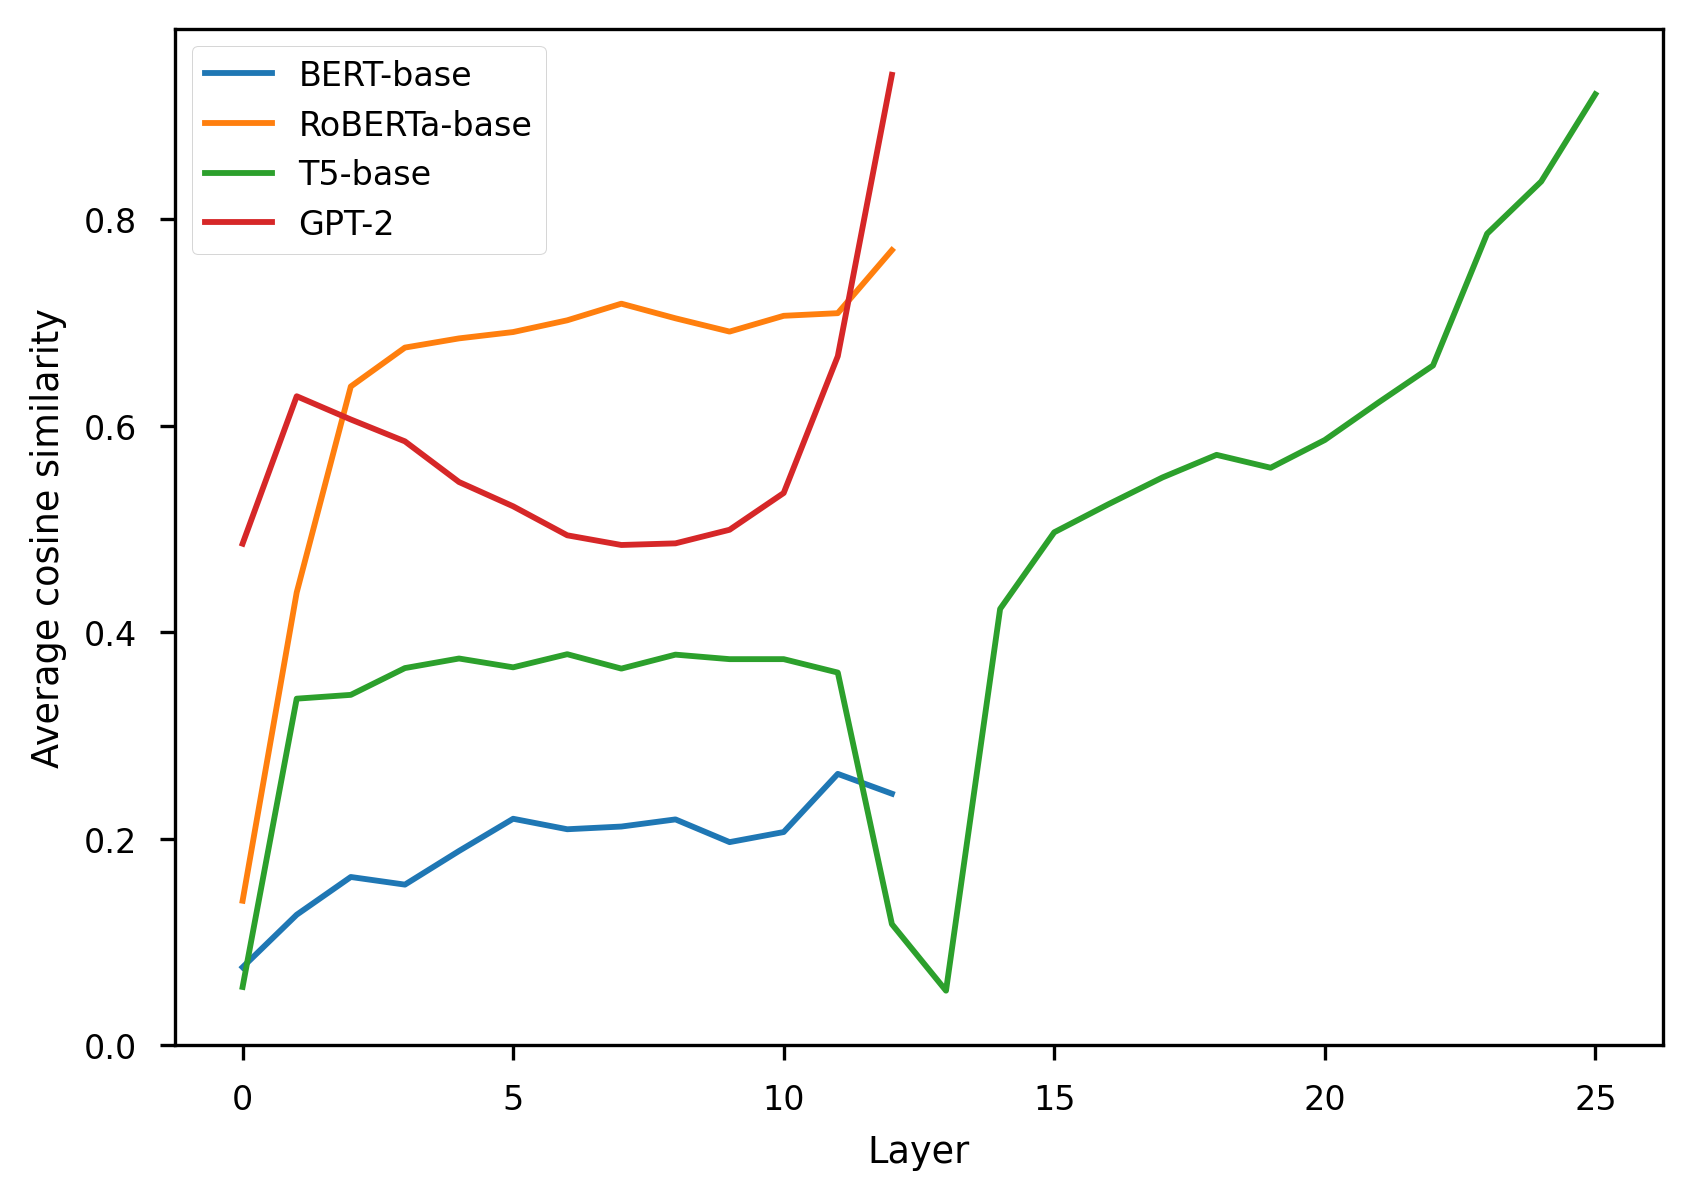
\includegraphics[width=0.6\columnwidth]{sources/part_1/anisotropy/imgs/cosine_token.png}
     \caption{Average cosine-similarity between hidden representations across layers for token-level NLP models. For T5-base, we concatenate encoder and decoder results.}
     \label{fig:anisotropy_token}
\end{figure}

As mentioned in \Cref{ssec:degeneration}, several works have established a connection between word frequency and distortions of the latent spaces \citep{yu-etal-2022-rare, puccetti-etal-2022-outlier,rajaee-pilehvar-2022-isotropy}. \citet{bis-etal-2021-much} have shown that anisotropy in LMs could be explained by a global \textit{drift} of the representations in the same direction, thus unifying conclusions from \citet{ethayarajh-2019-contextual} and \citet{gao2018representation}. The authors propose that this drift is caused by the persistent updating of the representation of rare and unused tokens in a consistent direction, due to the nature of the softmax operation in the cross-entropy loss. They show that removing the average component to all representations leads to a nearly perfect isotropy.

Various methods have been proposed to reduce anisotropy in Transformer-based LMs at token-level \citep{rajaee-pilehvar-2021-cluster, Wang2020Improving}, or at sentence-level \citep{gao-etal-2021-simcse, yan-etal-2021-consert,su2021whiteningsentencerepresentationsbetter} (see \Cref{sec:rw_sent_embs}). They usually consist in post-processing the representations, and lead to downstream performance boosts. We argue that these positive results are paving the way for the search of pre-training objectives that do not introduce anisotropy in the first place, in the hope that the resulting models will also perform better without any post-processing, and potentially be trained more efficiently. This motivates us to gain a deeper understanding of the underlying factors that induce anisotropy, whether they belong in data, architectures, or training procedures.



\section{Anisotropy in pre-trained Transformers}
\subsection{Character-based NLP}
\label{sec:charbased}
\begin{figure}[ht]
    \centering
     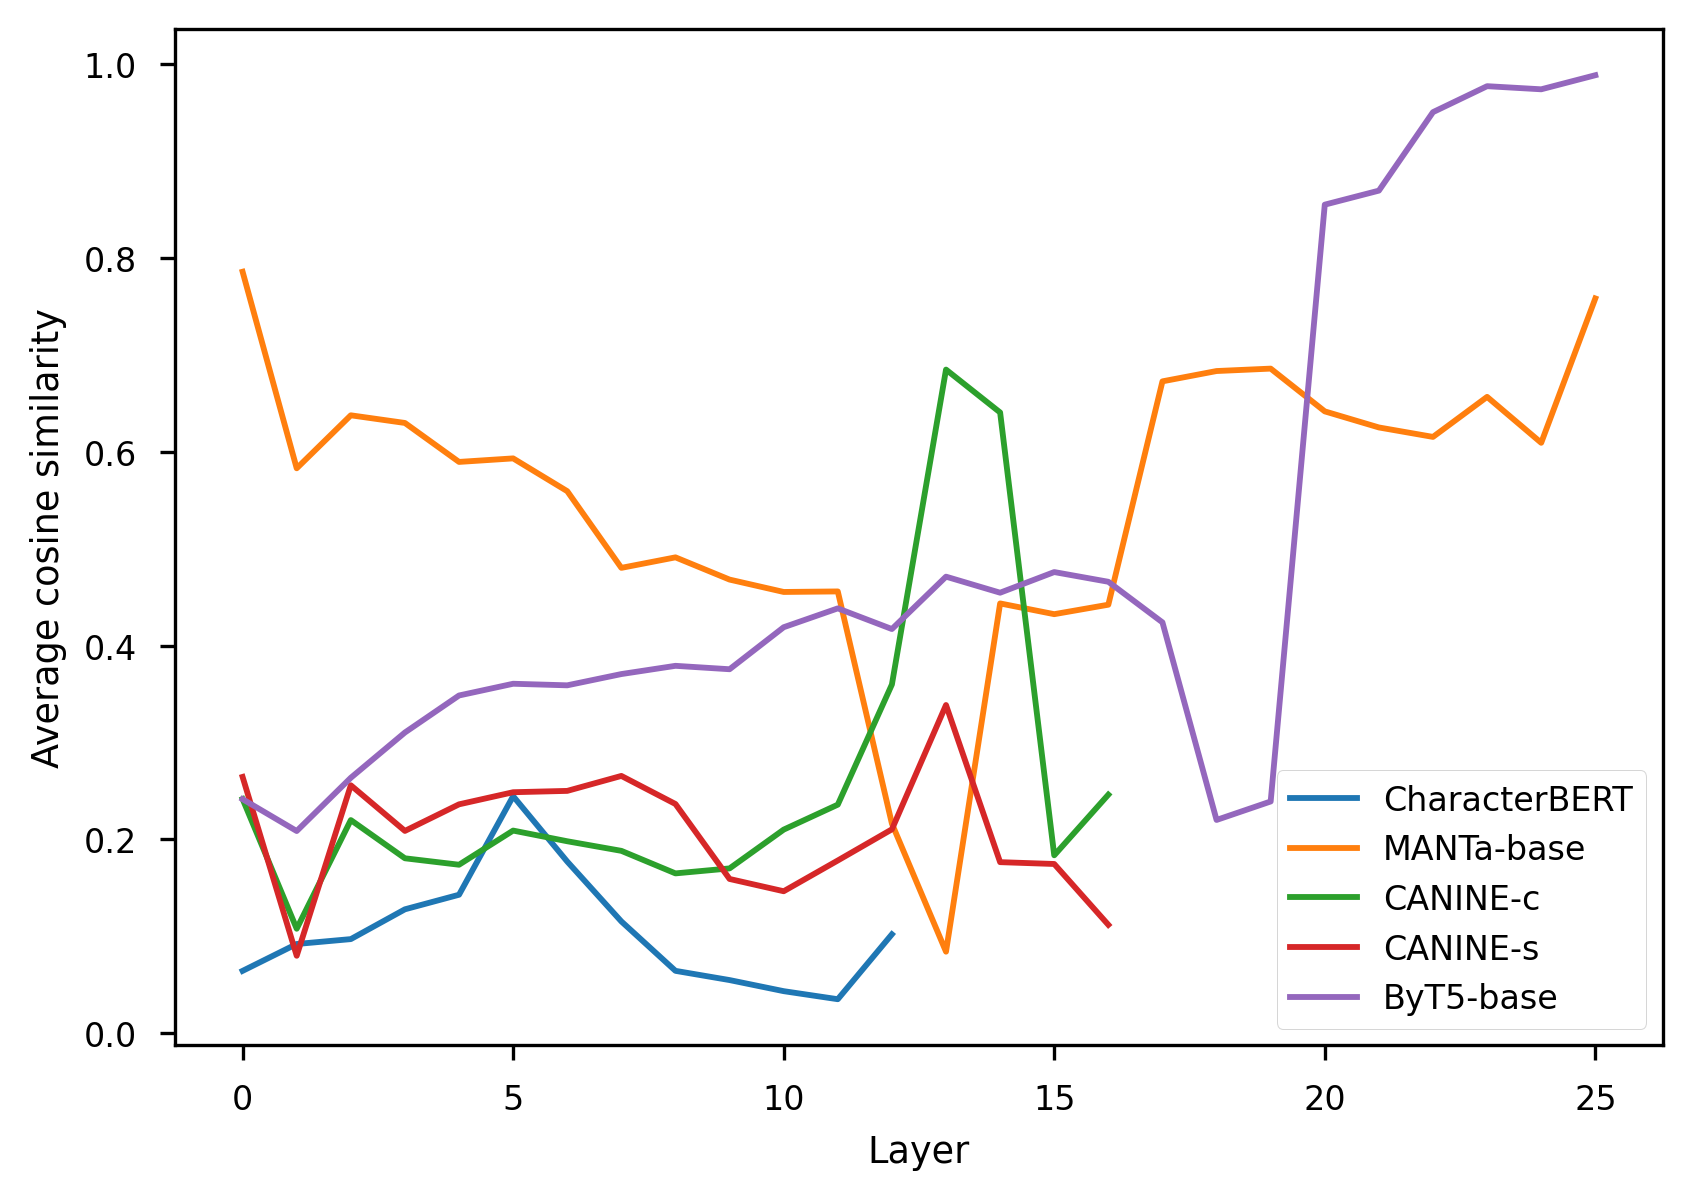
\includegraphics[width=0.6\columnwidth]{sources/part_1/anisotropy/imgs/cosine_char_based.png}
     \caption{Average cosine-similarity between hidden representations across layers for character-level models.}
     \label{fig:cos_char_aware}
\end{figure}

To assert whether the cross-entropy objective applied on vocabularies containing rare tokens is the sole cause for the common drift issue, we explore anisotropy in character-based models. We study different architectures presented in \Cref{sec:tokfree}, and our character-level model:
\begin{itemize}
    \item CharacterBERT \citep{el-boukkouri-etal-2020-characterbert} is constructing whole word representations from character embeddings put through convolutions and highway layers, before feeding them to a Transformers architecture.
    \item CANINE \citep{clark-etal-2022-canine} is downsampling contextualized character representations via a strided convolution before feeding them to a Transformers. It can be trained either with a subword-based objective (CANINE-s) or with a character-level one (CANINE-c).
    \item MANTa-LM (see \Cref{chap:manta}) is based on a differentiable segmentation and embedding module added before an encoder-decoder model in the style of T5 \citep{2020t5}. It takes bytes as inputs and outputs, but builds internal representations that are usually based on several bytes.
    \item ByT5 \citep{xue-etal-2022-byt5} is a version of T5 that is trained at byte-level. To afford for more complex encoding, the authors resize the encoder-decoder architecture.
\end{itemize}

Neither of these architectures should suffer from out-of-vocabulary tokens in the process of creating representations. The models that predict at word or sub-word level (CharacterBERT and CANINE-s) could have the cross-entropy loss systematically pushing away rare item representations. However, it is rather unclear why this would imply an embedding drift for deeper layers. Hence, if anisotropy was only caused by the presence of unused or rare subwords, those character-level models should be much less prone to this issue.

To verify this hypothesis, we compute hidden representations for the validation set of the WikiText-103 corpus \citep{merity2017pointer}. We then compute the average cosine-similarity between two representations, uniformly taken in the whole validation corpus.

In fact, as shown in \Cref{fig:cos_char_aware}, those models all display significant levels of anisotropy in at least one of their layers. Interestingly, the models that are based solely on characters or bytes for input and prediction (ByT5, CANINE-c, and MANTA-LM) seem to display even higher levels of anisotropy. We note, as it is the case for the T5 model, that the ByT5 decoder displays extremely high levels of anisotropy.

\subsection{Other modalities}
\label{sec:other_mod}
\begin{figure*}[ht]
    \centering
    \begin{subfigure}[b]{0.43\textwidth}
         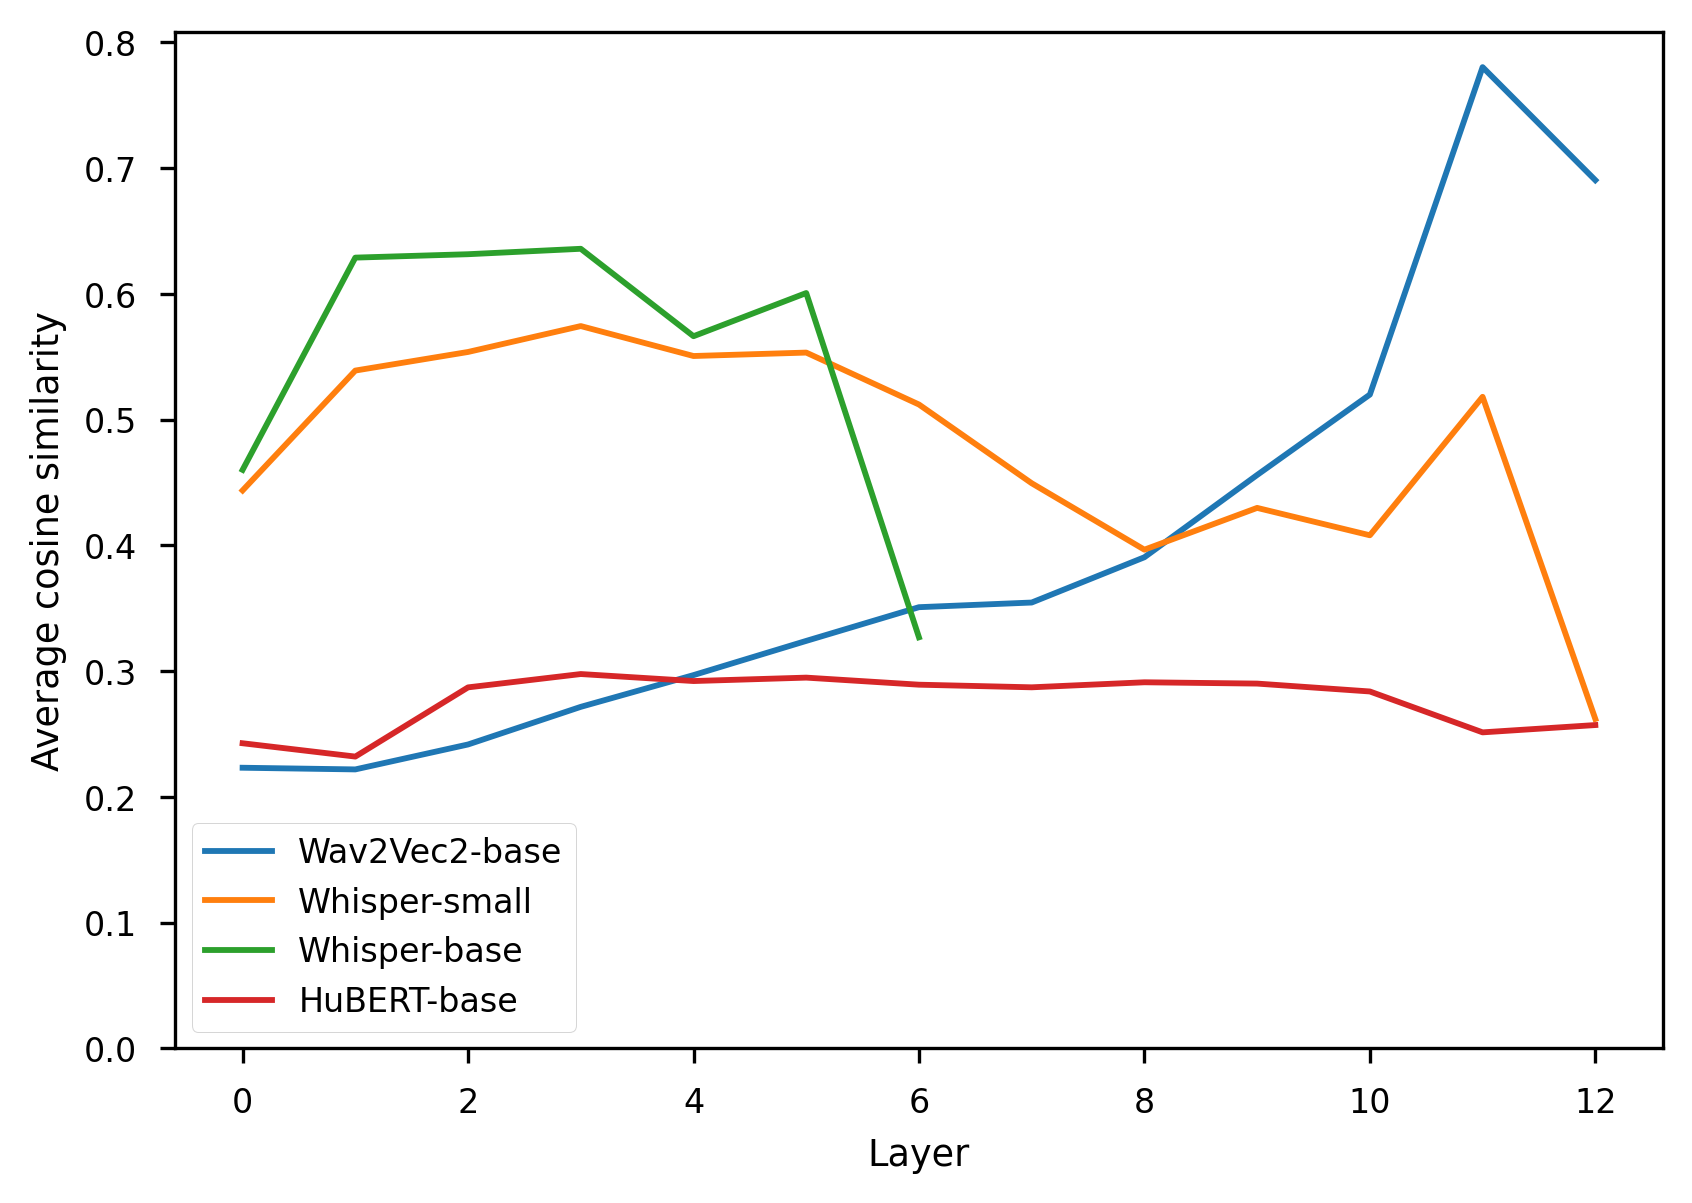
\includegraphics[width=\linewidth]{sources/part_1/anisotropy/imgs/cosine_audio.png}
         \caption{Speech}
         \label{fig:cos_speech}
    \end{subfigure}
    \hfill
    \begin{subfigure}[b]{0.43\textwidth}
         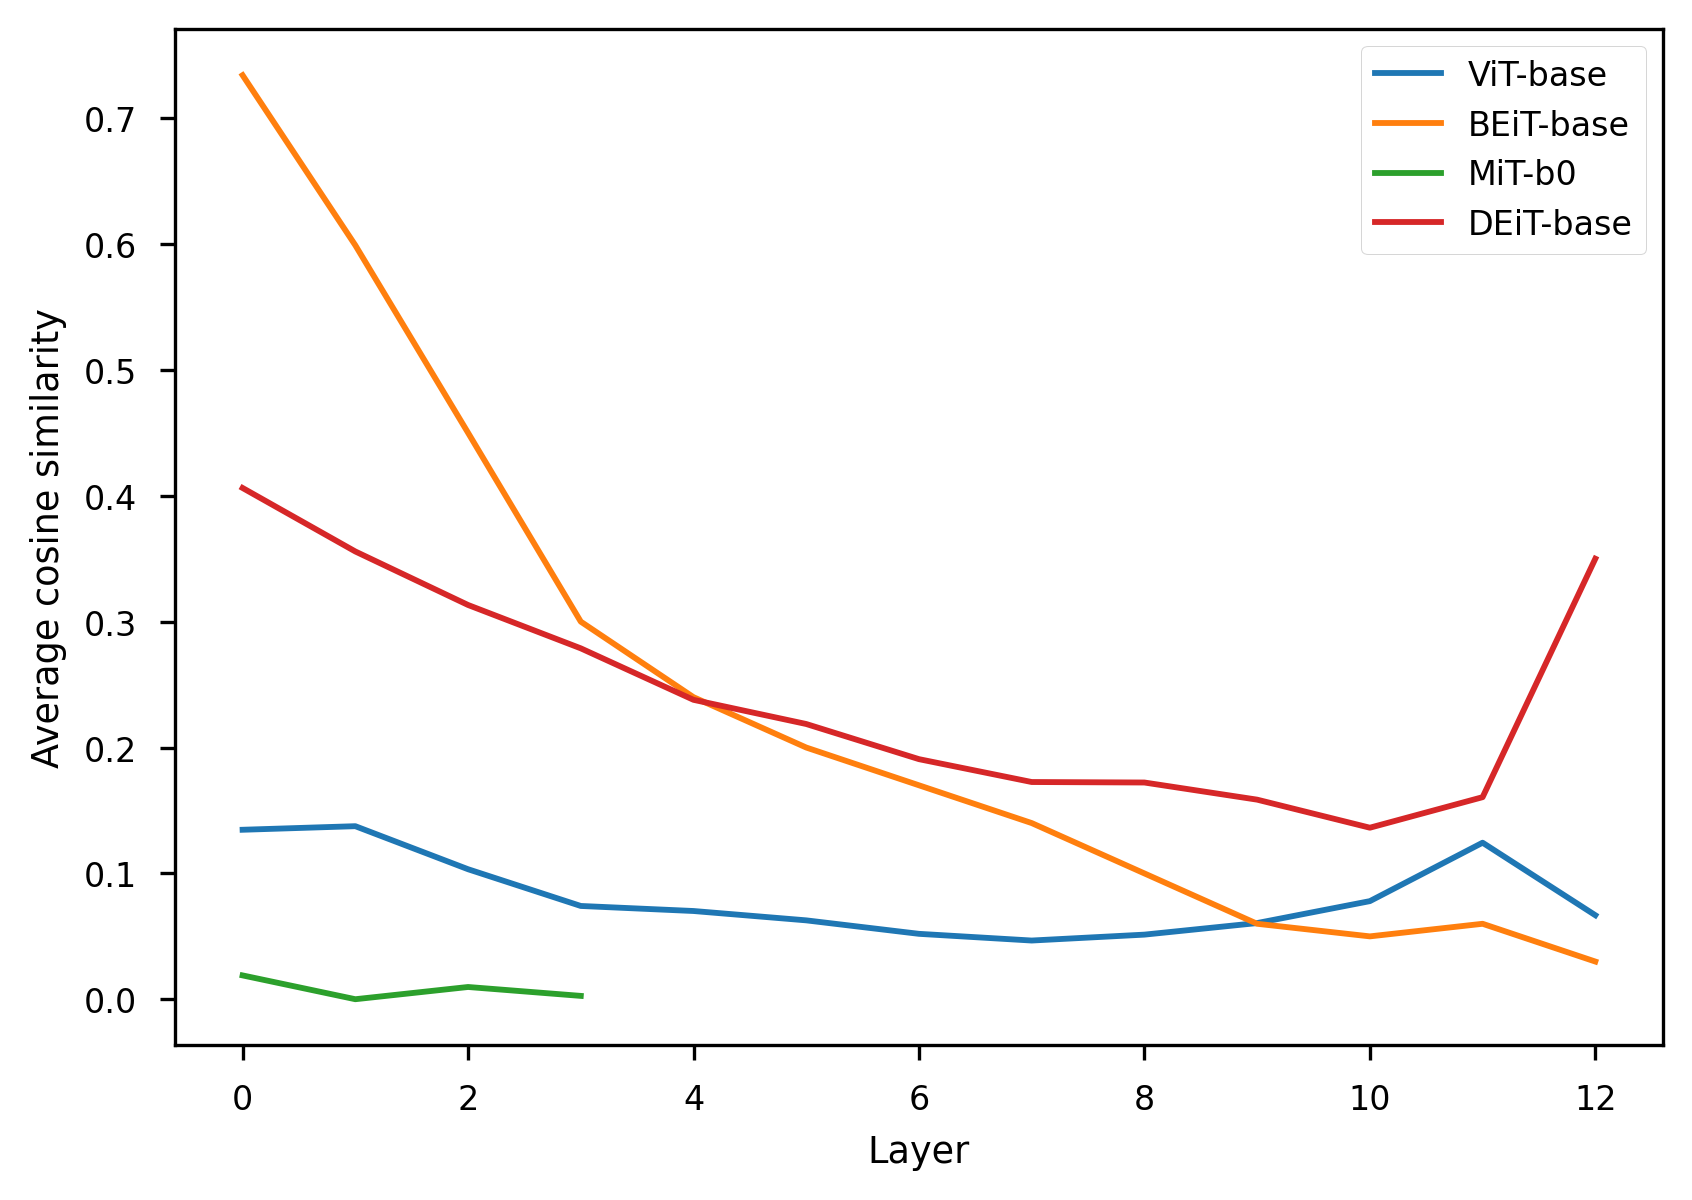
\includegraphics[width=\linewidth]{sources/part_1/anisotropy/imgs/cosine_vit_imagenet.png}
         \caption{Vision}
         \label{fig:cos_audio}
    \end{subfigure}
    \caption{Average cosine-similarity between hidden representations across layers for Speech and Vision modalities. We observe that across both modalities, several models display significant levels of anisotropy.}
    \label{fig:anisotropy_modalities}
\end{figure*}

We have shown in the previous section that character-level language models suffer from anisotropy similarly to token-level ones, hinting that subword token distributions are not solely responsible for anisotropy. Still, it may be argued that anisotropy is related to linguistic properties inherent to textual data. Thus, we proceed to explore the anisotropy problem for Transformers-based models in other modalities, specifically speech and vision.

For speech models, we consider wav2Vec 2.0 \citep{wav2vec}, HuBERT \citep{HuBERT}, and Whisper \citep{radford2022whisper} with the Common Voice 11.0 dataset \citep{commonvoice:2020}. For vision models, we use ViT \citep{Wu2020VisualTT}, BEiT \citep{beit-2021}, MiT \citep{segformer21}, and DEiT \citep{pmlr-v139-touvron21a} on the ImageNet dataset \citep{imagenet15russakovsky}.

As in \Cref{sec:charbased}, we infer hidden representations on the validation sets for each modality. We then uniformly sample pairs of vectors to get cosine-similarity values for every layer of every model. The averaged results are displayed in \Cref{fig:anisotropy_modalities}.

Once again, almost every model shows a significant level of anisotropy on some of its layers. Notably, speech models seem to have very anisotropic representations, as every layer of every model outputs an average cosine-similarity of at least $0.2$. We find some exceptions among vision models, since the MiT model seems to use isotropic representation spaces and the ViT model has a low average cosine-similarity for all its layers.

We also conduct the same experiment for convolution-based networks in the vision modality. The models at glance are ResNet \citep{he2016deep}, EfficientNet \citep{Tan2019EfficientNetRM}, CvT \citep{wu2021cvt}, ConvNeXt \citep{liu2022convnet}, and VAN \citep{guo2022visual}. For these networks, we flatten convolution maps to vectors before computing the cosine-similarity.

\begin{figure}[ht]
    \centering
    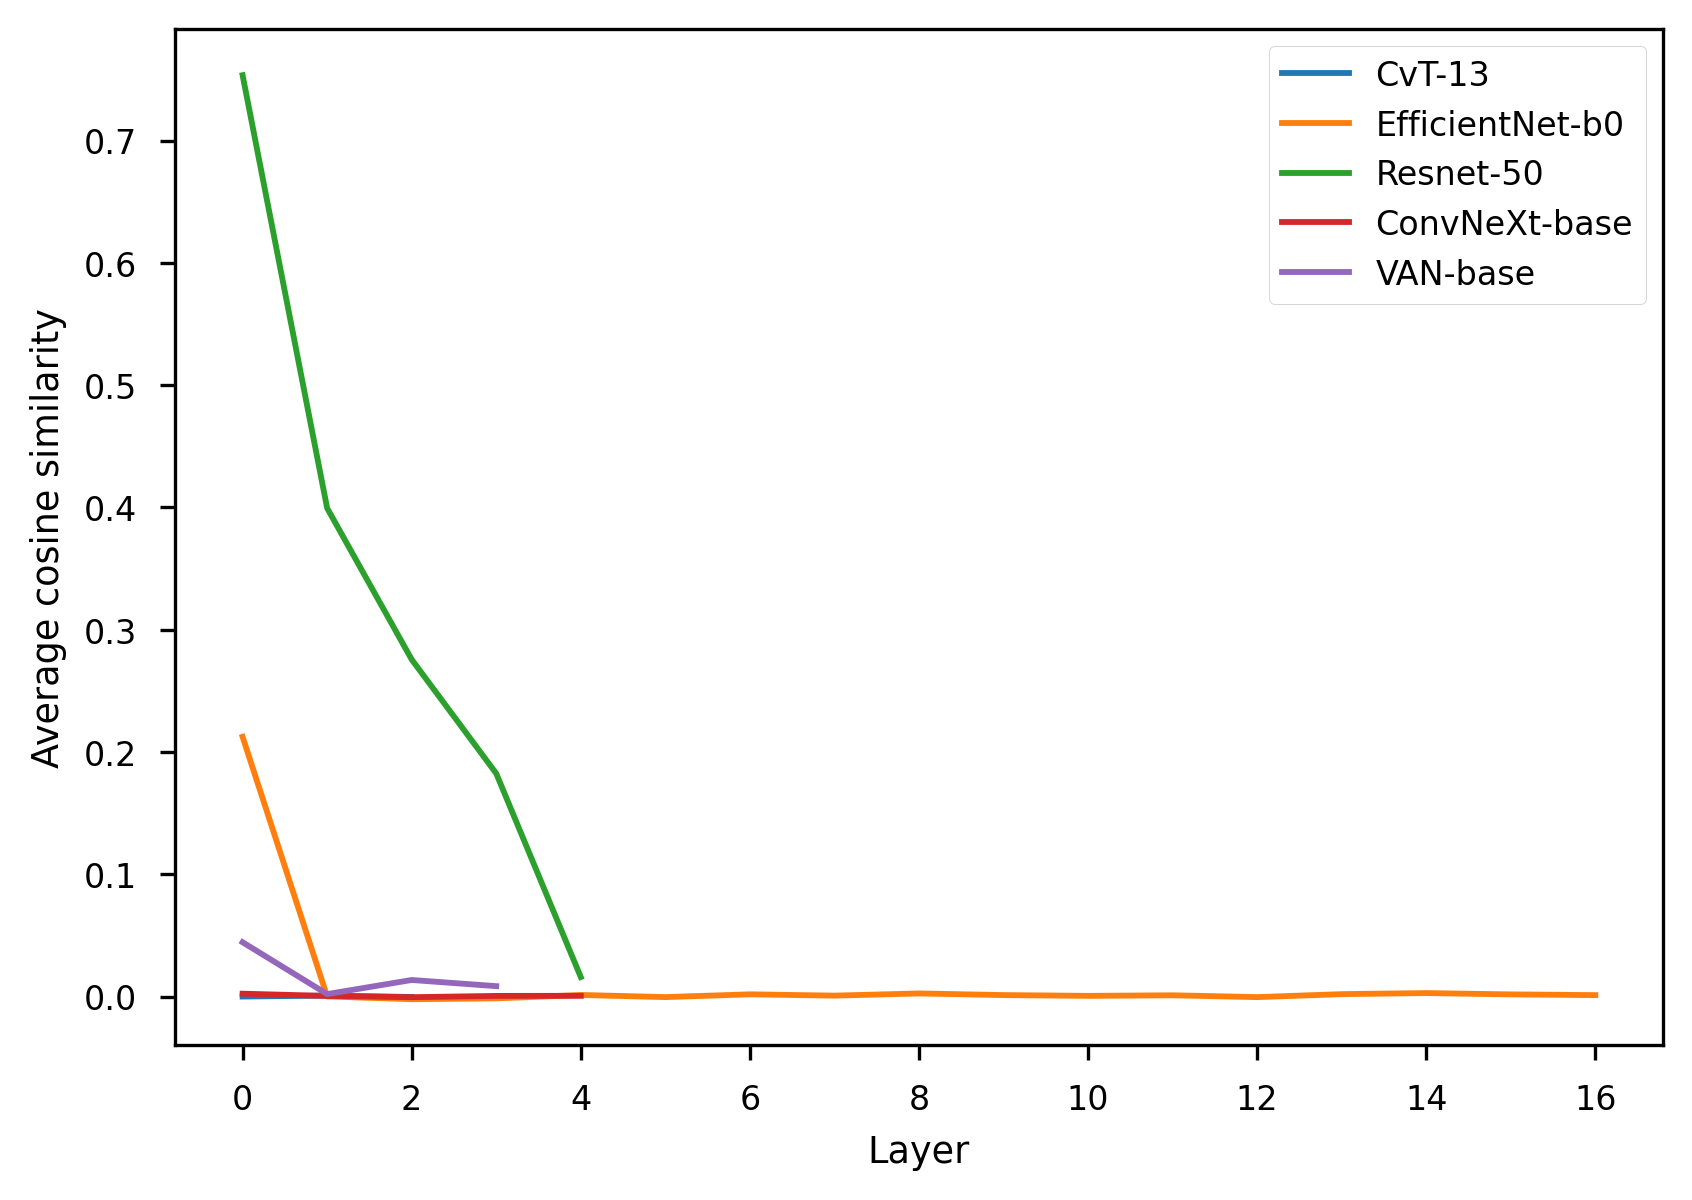
\includegraphics[width=0.6\linewidth]{sources/part_1/anisotropy/imgs/cosine_cnn_imagenet.png}
    \caption{Average cosine-similarity between hidden representations across layers for convolution-based vision models.}
    \label{fig:convbased}
\end{figure}

We observe in \Cref{fig:convbased} that most of the convolution-based models are isotropic. Interestingly, the only exception is ResNet-50, whose representations become more and more isotropic as one explores deeper layers. This could partially be explained by the fact that the batch normalization \citep{pmlr-v37-ioffe15} used in some of these models mitigates \textit{a posteriori} the drift effect by removing the mean component of the representations. However, the ConvNeXt model also seems to use isotropic representations while not using batch normalization, which shows that this is not the only factor in the isotropic behavior of these models.

\subsection{When is anisotropy ``high''?}

\begin{figure*}[ht]
     \centering
     \begin{subfigure}[b]{0.43\textwidth}
          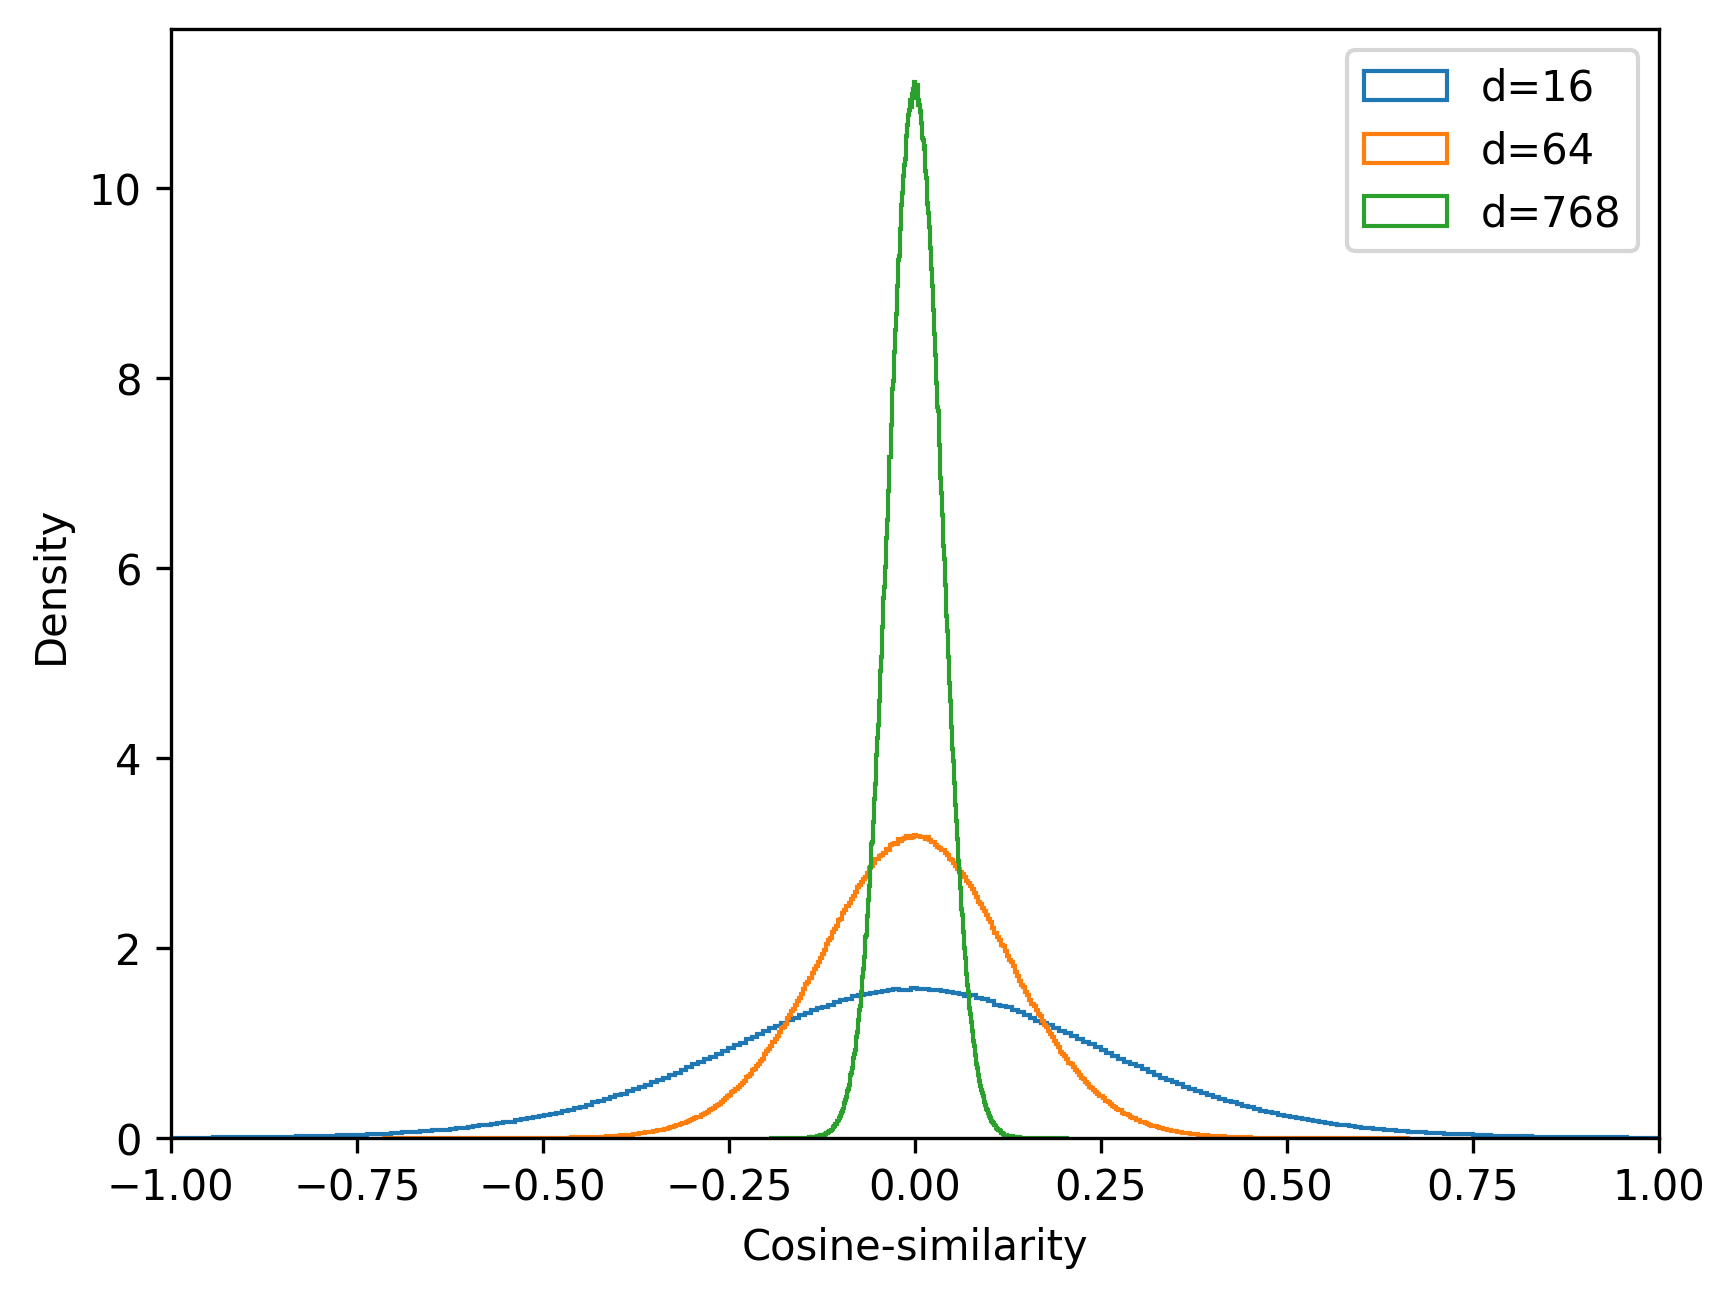
\includegraphics[width=\linewidth]{sources/part_1/anisotropy/imgs/cosine_v_density.png}
          \caption{Density function of cosine-similarity}
          \label{fig:cosine_v_density}
     \end{subfigure}
     \hfill
     \begin{subfigure}[b]{0.43\textwidth}
          \includegraphics[width=\linewidth]{sources/part_1/anisotropy/imgs/q95_dimension.png}
          \caption{95$^{\text{th}}$\! quartile of the cosine-similarity distribution}
          \label{fig:q95}
     \end{subfigure}
     \caption{Anisotropy metrics on multi-dimensional normal distributions as the dimension increases. In \Cref{fig:q95}, we add points for the average cosine-similarity level of Transformers models for several modalities.}
     \label{fig:anisotropy_high}
 \end{figure*}


It can be argued that describing anisotropy as the observation of ``high'' cosine-similarity values is not a convincing definition. This section aims at showing which ranges of cosine-similarity values are characteristic of anisotropic distributions. 
In \Cref{fig:cosine_v_density}, we show the density function of the cosine-similarity values obtained when drawing pairs of samples from isotropic normal distributions in $\mathbb{R}^d$ as $d$ increases. 

For smaller dimensions ($d=16$), we see that the range of cosine-similarity values that are reached between isotropic distributions is relatively broad compared to the possible spectrum ($[-1, 1]$). As $d$ increases, the support of the observed distributions seems to become smaller, due to the curse of dimensionality.

We analyze this effect more in-depth in \Cref{fig:q95}, where we plot the 95th quantile of the cosine-similarity distribution in the isotropic scenario. We also add values for the layer-wise average cosine-similarity levels of typical models in several modalities for comparison. We can clearly observe that the levels of cosine-similarity observed in the representations of Transformers-based models are significantly unlikely to be observed in between samples drawn in isotropic normal distributions.

Nevertheless, as we go towards higher dimensional spaces for bigger models (e.g. Llama-65B from \citet{touvron2023llama} has 8192 hidden dimensions), we believe that it may be relevant to introduce isotropy metrics that are grounded to isotropic cosine-similarity distributions. We leave this question for future works.

\subsection{To drift or not to drift?}
Related works \citep{bis-etal-2021-much, gao2018representation} show that anisotropy in subword-level language models is caused by a drift of the hidden representations in a shared direction. In this section, we try to extend this observation to other modalities.

We study the correlation between the uniformly measured cosine-similarity, and the norm of the average hidden representation $||\bar{h}||_2$ for each layer. If anisotropy could be directly explained by the drift effect, we would expect a monotonic relation between $||\bar{h}||_2$ and the average cosine-similarity. To verify this, we apply a Spearman correlation test on these two metrics for every model from \Cref{sec:charbased} and \Cref{sec:other_mod}, along with some token-level language models, namely T5 \citep{2020t5}, BERT \citep{devlin-etal-2019-bert}, RoBERTa \citep{roberta}, and GPT-2 \citep{gpt2}.

\begin{figure}[ht]
     \centering
     \begin{subfigure}[b]{0.43\columnwidth}
          \includegraphics[width=\linewidth]{sources/part_1/anisotropy/imgs/pval_vs_cosine_spearman.png}
          \subcaption{Spearman correlation test}
          \label{fig:pval_vs_cos_spearman}
     \end{subfigure}
     \hfill
     \begin{subfigure}[b]{0.43\columnwidth}
          \includegraphics[width=\linewidth]{sources/part_1/anisotropy/imgs/pval_vs_cosine_pearson.png}
          \subcaption{Pearson correlation test}
          \label{fig:pval_vs_cos_pearson}
     \end{subfigure}
     \caption{p-value of correlation tests between the norm of the average representation and the cosine-similarity averaged over all layers, across modalities. For models above the red dotted line, there is no significant ($p>0.05$) correlation between the drift effect and the anisotropy level.}
     \label{fig:pval_vs_cos}
 \end{figure}


In \Cref{fig:pval_vs_cos}, we observe that we can correlate the anisotropy level and the magnitude of the drift component across layers for several models. The anisotropy of subword-based models can generally be correlated with the drift effect using the Spearman correlation test, except for GPT-2 for which it may not be appropriate.

The Pearson test measures a linear correlation between random variables, while the Spearman test measures a monotonic correlation. As there is no specific argument in favor of a linear relationship between the measured distributions (average cosine-similarity and norm of the average representation), we decide to favour the Spearman correlation test in order to take into account more complex relation patterns.

Nevertheless, this metric is based on the rank of each observation, and is thus not robust to fluctuations due to sample variance, specifically when working with such small samples. This is reflected by the discrepancy between Pearson and Spearman p-values for some models (e.g. GPT-2). Hence, we report both metrics for completeness.

Interestingly, we notice that the anisotropy affecting most CNN-based vision models is generally not correlated with the drift effect, contrary to Tranformers-based models in the same modality. Some speech models (HuBERT and Whisper-base) also display signs of anisotropy that cannot be correlated with the drift effect. \Cref{fig:pval_vs_cos} also shows a correlation for all character-based models but Canine-C and MANTa-base.

\section{Exploring the representation drift}
\label{sec:empirical}
% We've empirically explored the extent of the anisotropy effect in Transformers-based models, and showed that it affects various modalities.
In this section, we focus on some intrinsic properties of the Transformer block in a modality-agnostic fashion, i.e. with minimal assumptions on the data distribution, and without training. We analyze experimentally the behavior of the untrained Transformer block $T$ when a common bias term $b$ is added to untrained input representations $\mathbf{h}$. This allows us to mimic the common drift as mentioned in \citet{bis-etal-2021-much} and to identify some properties induced by this artificial drift on the output representations.

\subsection{Experimental setup}
We consider an embedding lookup table $E$ and a Transformer block $T$ with weights initialized as in BERT \citep{devlin-etal-2019-bert}. We then draw 16 input embedding sequences $\mathbf{h}$ of length 512 uniformly from $E$. To account for a drift component of norm $\eta \in\mathbb{R}$, we generate a vector $b_u \sim \mathcal{N}(0, I_d)$, which we normalize into $b_\eta = \frac{b_u}{||b_u||_2}\cdot \eta$. We finally compute $T(\mathbf{h} + b)$ for every sequence $\mathbf{h}$, and study the resulting distributions.

Specifically, we study the average norm of the input representations $\mathbb{E}(||\mathbf{h} + b_\eta||_2)$ against the average norm of the output representations $\mathbb{E}(||T(\mathbf{h} + b_\eta)||_2)$ in \Cref{fig:norm_scratch_transformer}. We also retrieve the self-attention scores before the softmax operation, namely $\frac{Q^h{K^h}^T}{\sqrt{d_k}}$, along with the corresponding $Q^h$ and $K^h$ matrices. We study some of their properties in \Cref{fig:attscore_trained_transformer} and \Cref{fig:kq}.

\subsection{Input vs. output analysis}
\begin{figure}[ht]
    \centering
    \begin{subfigure}[b]{0.43\columnwidth}
         \includegraphics[width=\linewidth]{sources/part_1/anisotropy/imgs/scratch_bert_base_input_vs_output.png}
         \subcaption{Cosine similarity}
         \label{fig:cos_scratch_transformer}
    \end{subfigure}
    \hfill
    \begin{subfigure}[b]{0.43\columnwidth}
         \includegraphics[width=\linewidth]{sources/part_1/anisotropy/imgs/bert_base_norm_v_output.pdf}
         \subcaption{Norm}
         \label{fig:norm_scratch_transformer}
    \end{subfigure}
    \caption{Input/Output comparison of a Transformer block from BERT-base as the bias norms increases.}
    \label{fig:bias_vs_cosine_norm}
\end{figure}

In \Cref{fig:cos_scratch_transformer}, we observe that the output representations have an average cosine-similarity value that is slightly higher than the one of the input representations, no matter the level of input bias. We also notice that while the norm of the average output representation increases with the bias norm, it seems to meet the corresponding input measure for a given bias norm.

Interestingly, this shows that there is a \textit{fixed point} in terms of norm in the Transformers function with biased input. More formally, there seems to exist a bias norm $\eta^* \in \mathbb{R}_+$ such that: $$\mathbb{E}_{\mathbf{h}, b_{\eta^*}}(||\mathbf{h} + b_{\eta^*}||) = \mathbb{E}_{\mathbf{h}, b_{\eta^*}}(||T(\mathbf{h} + b_{\eta^*})||)$$

Moreover, this fixed point level $\eta^*$ is in the order of magnitude of the average hidden state norms of the layers of the trained BERT model. This hints that the model's representations stabilize when their norm is close to this fixed point. We leave a more thorough analysis of this hypothesis for future work.

\subsection{Exploring the Transformer block}

To understand the effect of the drift effect on the inner workings of the Transformer layer, we take a closer look at the self-attention operation as the average input representation drifts away.

\begin{figure}[ht]
    \centering
    \includegraphics[width=0.6\linewidth]{sources/part_1/anisotropy/imgs/trained_bert_base_att_scores.pdf}
    \caption{Histograms of the pre-softmax attention scores as the input bias norm increases. Other initializations of the layer and of the bias direction $b_u$ led to a general \textit{increase} of the attention scores instead.}
    \label{fig:attscore_trained_transformer}
\end{figure}

\Cref{fig:attscore_trained_transformer} shows that the attention scores tend to move away from zero as the input bias norm increases. Indeed, as the norm of the average $\bar{\mathbf{h}}$ of the input embeddings increases, we can expect the query and key vectors $Q^h$ and $K^h$ to also display signs of anisotropy. Actually, for each self-attention head, and for all position $i \in [1, L]$, we have:
\begin{equation}
    \begin{cases}
      \mathbb{E}_{\mathbf{h}}(Q^h_i) = W_{Q^h}\bar{\mathbf{h}} + b_{Q^h}\\
      \mathbb{E}_{\mathbf{h}}(K^h_i) = W_{K^h}\bar{\mathbf{h}} + b_{K^h}
    \end{cases}
\end{equation}

We can observe in \Cref{fig:kq} that query and key representations indeed increase in norm with the input bias norm. We also notice that the corresponding distributions are anisotropic even when no bias is added, which may be a consequence of BERT's initialization parameters.

\begin{figure}[ht]
    \centering
    \begin{subfigure}[b]{0.43\columnwidth}
         \includegraphics[width=\linewidth]{sources/part_1/anisotropy/imgs/trained_bert_base_bias_vs_kq_cos.png}
         \caption{Cosine similarity}
         \label{fig:cos_qk_trained_transformer}
    \end{subfigure}
    \hfill
    \begin{subfigure}[b]{0.43\columnwidth}
         \includegraphics[width=\linewidth]{sources/part_1/anisotropy/imgs/trained_bert_base_bias_vs_kq_norm.png}
         \caption{Norm}
         \label{fig:norm_qk_trained_transformer}
    \end{subfigure}
    \caption{Analysis of the self-attention query and key distributions}
    \label{fig:kq}
\end{figure}

\subsection{Impact of the drift}

After exploring the consequences of the drift of input representations on the query-key product in self-attention, we identify in this section the implications of this drift at a more explainable level, by observing the resulting post-softmax distributions.


\begin{figure}[ht]
    \centering
    \includegraphics[width=0.6\linewidth]{sources/part_1/anisotropy/imgs/untrained_bert_base_bias_vs_softmax.png}
    \caption{Evolution of the self-attention softmax values as the input bias norm increases.}
    \label{fig:softmax_trained_transformer}
\end{figure}

In \Cref{fig:softmax_trained_transformer}, we retrieve softmax values in the self-attention block and for each position, we extract the maximum, the median and the minimum. We then average these values over the whole batch, and repeat for various input bias norm levels. We notice that as the input bias norm increases, the self-attention softmax distributions tend to become less entropic, evolving towards higher maximal probabilities and lower minimal probabilities. In the following analysis, we'll use the term \textit{sharpness} to discuss entropy levels of the self-attention distributions.


\begin{figure}[ht]
    \centering
    \begin{subfigure}[b]{0.43\columnwidth}
         \includegraphics[width=\linewidth]{sources/part_1/anisotropy/imgs/untrained_bert_base_bias_vs_max_softmax.png}
         \caption{Maximum}
         \label{fig:max_softmax}
    \end{subfigure}
    \hfill
    \begin{subfigure}[b]{0.43\columnwidth}
         \includegraphics[width=\linewidth]{sources/part_1/anisotropy/imgs/untrained_bert_base_bias_vs_min_softmax.png}
         \caption{Minimum}
         \label{fig:min_softmax}
    \end{subfigure}
    \caption{Comparison of the extreme values of each sequence averaged over the batch as the bias norm increases.}
    \label{fig:min_vs_max}
\end{figure}

This sharpening effect of the attention distributions becomes even clearer if we consider the maximum and minimum values over the whole sequences, as in \Cref{fig:min_vs_max}.

However, at low anisotropy levels, i.e. when the bias norm is low, we see that the effect is not very important. \Cref{fig:softmax_trained_transformer} and \Cref{fig:min_vs_max} only hint at the fact that the drift of embeddings may help the self-attention to be sharper. Another explanation could be that training favors sharp self-attention patterns, as has been pointed out in previous works \citep{clark-etal-2019-bert}, which in turn induces a drift in the models' representations. In order to account for that, we need to study the evolution of latent spaces at the self-attention level along training.

\section{Queries and keys: training dynamics}
\label{sec:qk}
\begin{figure*}[ht]
    \centering
    \begin{subfigure}[b]{0.43\linewidth}
         \includegraphics[width=\linewidth]{sources/part_1/anisotropy/imgs/dist_l9h9_s0.png}
         \caption{Step 0}
         \label{fig:dist_qk_s0}
    \end{subfigure}
    \begin{subfigure}[b]{0.43\linewidth}
         \includegraphics[width=\linewidth]{sources/part_1/anisotropy/imgs/dist_l9h9_s40.png}
         \caption{Step 40k}
         \label{fig:dist_qk_s40}
    \end{subfigure}
    \begin{subfigure}[b]{0.43\linewidth}
         \includegraphics[width=\linewidth]{sources/part_1/anisotropy/imgs/dist_l9h9_s200.png}
         \caption{Step 200k}
         \label{fig:dist_qk_s200}
    \end{subfigure}
    \begin{subfigure}[b]{0.43\linewidth}
         \includegraphics[width=\linewidth]{sources/part_1/anisotropy/imgs/dist_l9h9_s2000.png}
         \caption{Step 2M (final)}
         \label{fig:dist_qk_s2M}
    \end{subfigure}
    \caption{Evolution of $Q^h_s$ and $K^h_s$ distributions along training (on layer $9$ and head $h=9$). Vectors are projected using a common SVD.}
    \label{fig:proj_qk_heads}
\end{figure*}

We have established that manually pushing for drift-based anisotropy on \textit{untrained} Transformers models leads to sharper (i.e. low-entropy) self-attention patterns. In this section, we show that this evolution of self-attention values actually takes place during training, and we explore the mechanism behind their appearance. As pointed out in \Cref{sec:empirical}, the self-attention scores result from the $Q^h(K^h)^T$ operation, which computes scalar products between query and key representations corresponding to each pair of positions. Thus, in this section, we study the evolution of these query and key representations \textit{along training}, and explore the mechanism behind the increase of the scalar products leading to self-attention scores.

We use the MultiBERT checkpoints \citep{sellam2021multiberts} with seed 0 to retrieve $Q^h$ and $K^h$ distributions at different pretraining steps, and we use 128 samples from Wikitext-103 as input data. Along this section, $Q^h_s$ and $K^h_s$ refer to query and key representations extracted at a specific layer and head at a given step $s$, and $\hat{Q^h_s}$ and $\hat{K^h_s}$ are the average representations, taken over all tokens in the sampled batch. By studying $\bar{Q^h_s}$ and $\bar{K^h_s}$, we aim at exploring the common (or context-agnostic) drifts of keys and queries distributions.

\begin{figure}[ht]
    \centering
    \begin{subfigure}[b]{0.43\columnwidth}
         \includegraphics[width=\linewidth]{sources/part_1/anisotropy/imgs/l0h3_samedir_QK.png}
         \caption{Similar}
         \label{fig:QK_simdir}
    \end{subfigure}
    \hfill
    \begin{subfigure}[b]{0.43\columnwidth}
         \includegraphics[width=\linewidth]{sources/part_1/anisotropy/imgs/l9h5_diffdir_QK.png}
         \caption{Opposite}
         \label{fig:QK_diffdir}
    \end{subfigure}
    \caption{Evolution of $\bar{Q^h_s}$ and $\bar{K^h_s}$ along training for two different heads in the network, projected via common SVD. Each arrow represents a checkpoint in the MultiBERT suite. We display typical examples of dynamics in same/opposite direction.}
    \label{fig:QK_dir}
\end{figure}

In \Cref{fig:proj_qk_heads} and \Cref{fig:QK_dir}, we compute a SVD of the union of $Q^h_s$ and $K^h_s$ for all steps $s$, so that the projection makes sense for both distributions across steps for visualization purposes \footnote{We actually uniformly sample 20\% of the whole set of representations to compute the SVD under reasonable memory constraints.}. As shown in our selected examples, we observe that the dynamics of $\bar{Q^h_s}$ and $\bar{K^h_s}$ tend to align along training, making the average of the distributions drift in either similar or opposite directions. The first dimension of the SVD seems to describe this common drift. Note that in $\mathbb{R}^{d_h}$ ($d_h = 64$ being the head dimension), such an alignment is very unlikely to happen randomly. Interestingly, \Cref{fig:QK_simdir} shows that the common direction dynamics appear in the first few steps, while the opposite direction dynamics of  \Cref{fig:QK_diffdir} only starts after 8\% of the total training steps.

\begin{figure*}[ht]
    \centering
    \begin{subfigure}[b]{0.43\linewidth}
         \includegraphics[width=\linewidth]{sources/part_1/anisotropy/imgs/l0_cosine_QK.png}
         \caption{Layer 0}
         \label{fig:cosine_qk_l0}
    \end{subfigure}
    \begin{subfigure}[b]{0.43\linewidth}
         \includegraphics[width=\linewidth]{sources/part_1/anisotropy/imgs/l4_cosine_QK.png}
         \caption{Layer 4}
         \label{fig:cosine_qk_l4}
    \end{subfigure}
    \begin{subfigure}[b]{0.43\linewidth}
         \includegraphics[width=\linewidth]{sources/part_1/anisotropy/imgs/l9_cosine_QK.png}
         \caption{Layer 9}
         \label{fig:cosine_qk_l9}
    \end{subfigure}
    \begin{subfigure}[b]{0.43\linewidth}
         \includegraphics[width=\linewidth]{sources/part_1/anisotropy/imgs/l11_cosine_QK.png}
         \caption{Layer 11}
         \label{fig:cosine_qk_l11}
    \end{subfigure}
    \caption{Evolution of cosine-similarity between $\bar{Q^h_s}$ and $\bar{K^h_s}$ along training. Each color represents one self-attention head. Steps are counted in thousands. We generally observe that almost all heads see $\bar{Q^h_s}$ and $\bar{K^h_s}$ align in common or opposite directions along training. In other words, the average components of keys and queries representations tend to align in self-attention heads, which maximizes the magnitude of the scalar product between two average representations. We run a similar experiment on all MultiBERT seeds in \Cref{fig:seeds_qk}, and obtain comparable results.}
    \label{fig:cosine_qk_heads}
\end{figure*}

To consolidate our observations, we compute the evolution of the cosine-similarity between $\bar{Q^h_s}$ and $\bar{K^h_s}$ along training in \Cref{fig:cosine_qk_heads}. We also display some projected $Q^h_s$ and $K^h_s$ distributions for several $s$ steps in \Cref{fig:proj_qk_heads}.

\Cref{fig:cosine_qk_heads} shows that the first layers display a common direction dynamic, as the cosine-similarity tends to increase, thus showing that \textbf{the key and query distributions drift along a similar direction} in average. The last layers seem to adopt an opposite direction dynamic, as the cosine-similarity between their mean key and query representations gets negative along training.

\begin{figure}[ht]
    \centering
    \begin{subfigure}[b]{0.43\columnwidth}
         \includegraphics[width=\linewidth]{sources/part_1/anisotropy/imgs/l3h8_scalar_QK.png}
         \caption{Similar}
         \label{fig:scalar_sim}
    \end{subfigure}
    \hfill
    \begin{subfigure}[b]{0.43\columnwidth}
         \includegraphics[width=\linewidth]{sources/part_1/anisotropy/imgs/l9h9_scalar_QK.png}
         \caption{Opposite}
         \label{fig:scalar_opp}
    \end{subfigure}
    \caption{Evolution of the scalar product between $\bar{Q^h_s}$ and $\bar{K^h_s}$ along training. Steps are in thousands.}
    \label{fig:scalar_QK}
\end{figure}

As shown in \Cref{fig:scalar_QK}, this drift induces an increase in the magnitude of scalar products obtained in the self-attention $Q^h{K^h}^T$ operation, thus facilitating the emergence of sharp patterns where attention focuses on specific tokens.

\begin{figure}[ht]
    \centering
    \includegraphics[width=0.6\linewidth]{sources/part_1/anisotropy/imgs/entropy_decay.png}
    \caption{Average entropy of the probability distributions corresponding to self-attention rows along training. Each curve corresponds to one layer.}
    \label{fig:entropy_decay}
\end{figure}

Finally, \Cref{fig:entropy_decay} describes the evolution of the average entropy in self-attention distributions. We observe that training induces an overall decay of the entropy for all layers, with different dynamics. This corresponds to sharper self-attention distributions. It is interesting to notice that the distributions in the first layers remain sharper than the ones in the last layers.

Overall, this section shows that drift anisotropy emerges in the query and key representations during the training of MultiBERT, as self-attention distributions become sharper. The drifts of queries and keys tend to align, thus increasing the magnitude of scalar products, and the general sharpness of self-attention.

Although this section focuses on the case of token-based NLP, we believe that strong attention patterns may be required when training Transformers across all modalities, potentially generating distortions in query and key distributions that account for the final observed anisotropy of the models. However, we could not extend experiments to other modalities due to the lack of released intermediate checkpoints, to the best of our knowledge.

\section{Discussion}
\label{sec:anisotropy_discussion}

In this work, we argue that the nature of data distributions is not solely responsible for the anisotropy observed in most hidden representations of Transformers-based models across modalities. As \Cref{sec:empirical} shows, untrained Transformers layers display a tendency towards anisotropy. Biased inputs tend to increase the variance of the attention scores and thus facilitate the emergence of sharp patterns in the self-attention mechanisms. We also show in \Cref{sec:qk} that along training, query and key distributions drift in parallel directions, which increases anisotropy in the inner representations of the Transformer layers, while allowing sharper attention patterns. As discussed in \citet{puccetti-etal-2022-outlier}, outlier dimensions in Transformers are also involved in the emergence of strong attention patterns.

\paragraph{Consistency of the SVD} In \Cref{sec:qk}, we use an SVD on the \textit{union} of $Q^h_s$ and $K^h_s$ for visualization purposes (see \Cref{fig:proj_qk_heads} and \Cref{fig:QK_dir}). It may be argued that this approach favors the emergence of a discriminative singular direction, that helps distinguish between keys and queries, thus supporting the findings in a less convincing way. To address this concern, we display alternative projections in \Cref{sec:other_projs}, where we compute the SVD on $Q^h_s$ or $K^h_s$ only, and then project all representations using this SVD. Our observations show that our findings are consistent for these alternative projections.

\paragraph{Harmfulness of anisotropy} Even though anisotropy has not been shown to be an issue in language modeling, previous works have advocated that removing anisotropy in output representations leads to better sense disambiguation abilities \citep{bihani-rayz-2021-low, bis-etal-2021-much}. Isotropic models could also improve cross-lingual alignment in multilingual language models \citep{hämmerl2023exploring}. Nevertheless, concurrent works have suggested that anisotropy may not hurt the quality of the representations \citep{ait-saada-nadif-2023-anisotropy, rudman2023stable}. We argue that anisotropy in the Transformer architecture may actually help models by allowing sharp attention patterns, but we also believe that our work can pave the way for new architectures that can easily use sharp attention patterns without inducing anisotropy. 


\section*{Conclusion}
In this paper, we investigated the anisotropy problem through the lens of the drift effect, and made several contributions to the understanding of this phenomenon. We demonstrated that anisotropy can be observed in language models with character-aware architectures, extended our observations to Transformers trained on other modalities, and studied anisotropy in untrained Transformers layers. We finally explored the training dynamics of the query and key distributions, and found that they drift along a shared direction hence maximizing $Q^h{K^h}^T$ scalar products in absolute value, allowing stronger attention patterns as a result.

We conclude that anisotropy almost systematically affects Transformers on all modalities, in a way that is not always correlated with the drift of the representations. We also provide empirical evidence that anisotropy appears as an inherent property of latent distributions used in the self-attention mechanism when modeling sharp attention patterns. We hypothesize that a revision of the self-attention operation could help reduce anisotropy by facilitating the emergence of sharp attention softmax distributions without distorting the geometry of the hidden representations.


\section*{Limitations}
As mentioned in \Cref{sec:anisotropy_discussion}, we acknowledge that \Cref{sec:empirical} does not take into account the training dynamics, and only exposes some properties of the Transformer layer at initialization.

Moreover, we are aware that our approach is not theoretically rigorous in some aspects. For instance, we don't prove that sharp self-attention patterns \textit{cannot} emerge without anisotropy in keys and queries representations. In other words, this article is focusing on exposing and \textit{correlating} factors that explain anisotropy, but we do not demonstrate theoretical properties that would help identify the \textit{causes} of anisotropy. Nevertheless, we believe that our work can pave the way for such theoretical exploration in the future.

\vspace{2em}

In this section, we show that representation degeneration happens in the self-attention layers and co-occurs with the sparsification of attention patterns, regardless of the data modality. This incentivizes the analysis of representation geometry as a way to better understand these implicit biases and paths towards how to improve them. 


% \section*{Ethics Statement}
% To the best of our knowledge, our work does not raise any ethical concern. However, as noted in \citet{zhou2021freqbased}, we believe that distortions in the embedding space may be related to bias in the training data, whether it is inherent to the structure of the modality (e.g. the Zipfian distribution of words), or due to human factors (e.g. geographical considerations).




\chapter*{Conclusion}

Overall, studying distortions and biases in the representation space has allowed us to shed light on bottlenecks and limitations that are inherent to the classical language modeling framework. It also provided insights about the architecture of modern language models, from the dimensionality and sparsity perspectives. 

Beyond the scope of usual interpretability frameworks, that are designed to explain predictions from targeted observations, we advocate for tools that allow analyzing global behaviors of the inner states of language models, in order to provide guidelines towards better paradigm for learning models of natural language.

Finally, we underline that our work, especially \Cref{chap:geobias} and \Cref{chap:softmax_bottleneck}, shows that representation degeneration and frequency-related biases hurt the quality of affected language models, either by degrading their performance or incorporating knowledge bias. In \Cref{part:solutions}, we propose several methods aimed at avoiding degeneration, reducing frequency dependency and mitigating sparsity in language models, in the hope that these methods will indirectly mitigate the identified limitations that are correlated with these phenomena.

% %%%%%%%%%%%%%%%%%%%%%%%%%%%%%%%%%%%%%%%%%%%%%%%%%%%%%%%%%%%%%%%%%%%%%%%%
\section{Representation Learning}
%%%%%%%%%%%%%%%%%%%%%%%%%%%%%%%%%%%%%%%%%%%%%%%%%%%%%%%%%%%%%%%%%%%%%%%%
\begin{center}
  \begin{minipage}{0.5\textwidth}
    \begin{small}
      In which the reasons for creating this package are laid bare for the
      whole world to see and we encounter some usage guidelines.
    \end{small}
  \end{minipage}
  \vspace{0.5cm}
\end{center}

\subsection{Introduction}


%%%%%%%%%%%%%%%%%%%%%%%%%%%%%%%%%%%%%%%%%%%%%%%%%%%%%%%%%%%%%%%%%%%%%%%%
\subsection{Statistical approaches}
%%%%%%%%%%%%%%%%%%%%%%%%%%%%%%%%%%%%%%%%%%%%%%%%%%%%%%%%%%%%%%%%%%%%%%%%
Statistical approaches to representation learning primarily involve methods that leverage co-occurrence statistics and distributional properties of words. Key techniques in this category include:

\begin{itemize}
  \item Latent Semantic Analysis (LSA): LSA is based on the Singular Value Decomposition (SVD) of term-document matrices, reducing the dimensionality of the data and uncovering latent semantic structures. By mapping words and documents to a shared vector space, LSA captures semantic similarities based on co-occurrence patterns.
\end{itemize}


Latent Dirichlet Allocation (LDA): LDA is a generative probabilistic model that represents documents as mixtures of topics, where each topic is a distribution over words. By inferring the topic distribution for each document, LDA provides a way to represent documents in a lower-dimensional topic space.

Word2Vec: Introduced by Mikolov et al., Word2Vec includes two model architectures—Continuous Bag of Words (CBOW) and Skip-gram. These models learn word embeddings by predicting the context words surrounding a target word or vice versa. The resulting vectors capture semantic relationships such as analogies (e.g., "king" - "man" + "woman" $\simeq$ "queen").

GloVe (Global Vectors for Word Representation): GloVe is another word embedding technique that combines the advantages of matrix factorization and local context window methods. It constructs a word-word co-occurrence matrix and derives word vectors by factorizing this matrix, ensuring that the dot product of word vectors approximates the logarithm of their co-occurrence probabilities.

%%%%%%%%%%%%%%%%%%%%%%%%%%%%%%%%%%%%%%%%%%%%%%%%%%%%%%%%%%%%%%%%%%%%%%%%
\subsection{Auto-encoders}
%%%%%%%%%%%%%%%%%%%%%%%%%%%%%%%%%%%%%%%%%%%%%%%%%%%%%%%%%%%%%%%%%%%%%%%%
Auto-encoders are neural network models designed to learn efficient representations of data through unsupervised learning. They consist of an encoder that maps input data to a latent space and a decoder that reconstructs the original data from this latent representation. In NLP, auto-encoders can be used to learn embeddings for words, sentences, or documents.

Basic Auto-Encoders: The simplest form of auto-encoders involves a single hidden layer that compresses the input into a lower-dimensional latent space. The model is trained to minimize the reconstruction error between the input and the output.

Variational Auto-Encoders (VAEs): VAEs extend basic auto-encoders by imposing a probabilistic structure on the latent space. They use a probabilistic encoder to map inputs to a distribution in the latent space, allowing for the generation of new samples by sampling from this distribution. VAEs are useful in tasks requiring generative capabilities, such as text generation.

Denoising Auto-Encoders (DAEs): DAEs are trained to reconstruct the original data from corrupted versions. This process encourages the model to learn robust features that are invariant to noise, improving the quality of the learned representations.

\subsection{Contrastive approaches}

Contrastive approaches in representation learning aim to learn effective embeddings by contrasting positive and negative examples. The core idea is to bring similar items closer together in the embedding space while pushing dissimilar items apart. These methods are essential for capturing nuanced relationships in the data and enhancing the quality of learned representations.
\begin{itemize}
  \item Contrastive Loss: The fundamental concept in contrastive learning is the contrastive loss function, which drives the learning process by encouraging the model to distinguish between positive pairs (similar items) and negative pairs (dissimilar items).
  \item Triplet Loss: Triplet loss is a popular contrastive learning technique that uses triplets of samples: an anchor, a positive (similar to the anchor), and a negative (dissimilar to the anchor). The objective is to minimize the distance between the anchor and the positive while maximizing the distance between the anchor and the negative. This approach is widely used in tasks such as face recognition and text similarity.
  \item 
  Noise Contrastive Estimation (NCE): NCE is another contrastive learning method that reformulates the problem of estimating a probability distribution into a binary classification problem. The model learns to distinguish between observed data and artificially generated noise samples. NCE is particularly useful in large-scale language models where direct computation of probabilities is computationally expensive.
\end{itemize}
% %%%%%%%%%%%%%%%%%%%%%%%%%%%%%%%%%%%%%%%%%%%%%%%%%%%%%%%%%%%%%%%%%%%%%%%%
\section{Language Modeling}
%%%%%%%%%%%%%%%%%%%%%%%%%%%%%%%%%%%%%%%%%%%%%%%%%%%%%%%%%%%%%%%%%%%%%%%%


%%%%%%%%%%%%%%%%%%%%%%%%%%%%%%%%%%%%%%%%%%%%%%%%%%%%%%%%%%%%%%%%%%%%%%%%
\subsection{Introduction}
%%%%%%%%%%%%%%%%%%%%%%%%%%%%%%%%%%%%%%%%%%%%%%%%%%%%%%%%%%%%%%%%%%%%%%%%
A language model is a probabilistic model that predicts distributions over textual units conditioned on a context. Typically, these textual units will be subwords (or \textit{tokens}), noted as $(w_t)_{t\in[1, L]}$, and the language model (or \textit{LM}) predicts the following probability:
$$
P(w_T | w_{\neq T})
$$
where the context $w_{\neq T}$ is a subset of subwords taken from $(w_t)_{t\in[1, L] \setminus T}$.

These models can be used in various applications, which will often shape the way the context is built. For instance, for text generation purposes, the context will be a subset of textual units from the past that we can write as $w_{< T}$, as the model can only access text that has already been generated. Conversely, for a language correction system, it is possible to build language models that use every element of $(w_t)_{t\in[1, L] \setminus T}$ as the text already exists when the system is used.


%%%%%%%%%%%%%%%%%%%%%%%%%%%%%%%%%%%%%%%%%%%%%%%%%%%%%%%%%%%%%%%%%%%%%%%%
\subsection{Methods}

\paragraph*{Textual units and Tokenization} Before presenting the statistical paradigm of modern language models, we need to define precisely the textual units on which these models are based, namely tokens. \citet{mielke2021wordscharactersbriefhistory} cope with this subject in a very exhaustive manner. They distinguish three different approaches of forming tokens: a linguistic approach, an atomic approach, and a statistical approach.

First, many works have built linguistically-grounded sets of textual units that should be considered as microscopic to some extent, such as the Morphosyntactic Annotation Framework \citep{clement_maf}, which defines a token as a \textit{non-empty contiguous sequence of graphemes or phonemes in a document}. More generally, the domain of morphology, well defined in \citet{aronoff2022morphology}, has led to several morphologically-informed tokenizers \citep{saleva-lignos-2021-effectiveness, gronroos-etal-2018-cognate}.

The atomic approach takes a radically different stance. It consists in using shorter units, e.g. bytes, characters or pixels from a rendered text (see \Cref{sec:tokfree}). Although this choice seems less biased and restrictive than the latter, it immediately raises computational complexity concerns in LMs, as the necessary number of units can considerably increase.

Paying attention to the number of units used for a given text utterance logically leads to techniques that statistically optimize for this metric while keeping a meaningful segmentation scheme in order to maintain the feasibility of language modeling. 

\begin{figure}[h]
    \centering
    \includegraphics[width=0.5\linewidth]{sources/related_works/imgs/token_graph.pdf}
    \caption{}
    \label{fig:token_graph}
\end{figure}

Such statistical methods have dominated in the last few years as the default way to encode textual data, the most used being BPE \citep{sennrich-etal-2016-neural}, WordPiece \citep{wu2016google} and Unigram \citep{kudo-2018-subword}.

Byte-Pair Encoding, or BPE \citep{Gage1994bpe}, is a compression technique that relies on recursive symbol merges. In NLP, it is based on a dataset that consists in sequences of characters or bytes, and it iteratively registers a set of merge operations that reduce the count of merged items the most. WordPiece \citep{wu2016google} is based on a similar concept but uses a different rule for selecting merges. The possible merges $ab$ are scored according to:

$$
s(ab) = \frac{f_{ab}}{f_a \times f_b}
$$

where $f_{x}$ is the frequency of the string $x$ in the dataset. This scoring function differs from the basic BPE frequency as it favors merges $ab$ that appear in most cases when $a$ or $b$ appear. This typically leads to a more linguistically meaningful segmentation, as prefixes and suffixes are less prone to merging.

The Unigram tokenization algorithm \citep{kudo-2018-subword} works in the opposite direction : it first creates an exhaustive list of token candidates, and then iteratively removes tokens that affect the likelihood of the segmented sequence the least once discarded.

The statistical approaches are widely used in modern LMs, sometimes jointly with techniques such as subword regularization \citep{provilkov-etal-2020-bpe} that diversify segmentation results.

\paragraph*{Likelihood Maximization} Once the tokenization scheme is chosen, textual documents are parsed into sequences of tokens taken from a vocabulary of possible tokens  $\mathcal{V}$ of size $\left|\mathcal{V}\right| = V$. A \textit{training set} $T = (s_i)_{i\in[1, S]}$ of $S$ token sequences is thus built from the target textual documents. Each of these sequences $s_i$ has a given length $l_i$, and can also be written $s_i = (w_j)_{j \in [1, l_i]}$.

A language model $\phi_\theta$, based on a parameter set $\theta$, is a function that takes a sequence of tokens $\mathbf{w}_{\neq t}$ called context as an input, and outputs a probability distribution in $\Delta ^V$ for the token at position $t$.

The performance of a language model at token-level can be measured by computing the probability of the realization $w_t$ in the context $\mathbf{w}_{\neq t}$:
$$
\phi_\theta(\mathbf{w}_{\neq t})_{w_t} = P_\theta(w_t | \mathbf{w}_{\neq t})
$$

The process of training a language model consists in optimizing its average performance on the training set, which can be framed as a likelihood maximization objective \citep{mle}. In practice, to improve numerical stability, the objective is based on log-likelihood :
$$
\theta^* = \argmax_{\theta} E_T(\log \phi_\theta(\mathbf{w}_{\neq t})_{w_t})
$$

The minimized likelihood can also be seen as cross-entropy minimization between $P_\theta$ and an observed contextual probability distribution, estimated from the sample at position $t$, which is $\mathbf{1}_{w_t}$.

A metric that is often used to evaluate language modeling performance is \textit{perplexity} :
$$
\mathcal{P}(\phi_\theta, t) = 2^{-\log \phi_\theta(\mathbf{w}_{\neq t})_{w_t}}
$$


\subsection{Architectures}

\paragraph*{Statistical Methods}

The straightforward approach to language modeling consists in statistically estimating the distribution of tokens based on their context. 

In its most basic form, such statistical model estimates the \textit{unigram} distribution, that is the non-contextual distribution $P(w_t)$. This distribution is estimated by bin-counting tokens in the training dataset $T$ to retrieve token frequencies $f_w$ for each token $w$, and setting :
$$
\phi_{\theta}(\mathbf{w}_{\neq t}) = (f_w)_{w \in \mathcal{V}} \in \Delta^{V}
$$

We can extend this idea by estimating the \textit{2-gram} distribution $P(w_{t-1}w_t)$. To do so, we count the occurences of the subsequence $w_{-1} w_0$ in the training dataset for each pair of tokens $w_{-1}, w_0 \in \mathcal{V}^2$. Doing so, we can build a $V \times V$ stochastic matrix - i.e. which coefficients are non-negative reals that sum to $1$ column-wise - containing the observed frequencies for $w$ in pairs of the form $w_{-1} w$:
$$
M_2(T) = (f_{w_{-1} w})_{w_{-1}, w \in V^2}
$$
Then, the language model $\phi_{\theta}$ becomes:
$$
\phi_{\theta}(\mathbf{w}_{\neq t}) = (f_{w_{t-1} w})_{w \in V}
$$

More generally, $n$-gram language models \citep{jurafsky_course} can be designed to estimate the distribution $P(w_{t-n +1}...w_{t-1}w_t)$. By bin-counting $n$-uplet occurences in $T$, one can compute:
$$
M_n(T) = (f_{w_{-n+1}...w_{-1}w})_{(w_{-n+1}...w_{-1}), w \in V^{n-1} \times V}
$$
The associated language model $\phi_{\theta}$ can then be written:
$$
\phi_{\theta}(\mathbf{w}_{\neq t}) = (f_{w_{t-n+1}...w_{t-1} w})_{w \in V}
$$

These $n$-gram language models can be combined with backoff strategies to take sample size into accounts and switch between $n$ values when appropriate \citep{kneser_ney}.

\paragraph*{Neural Methods}
\citet{bengio2000neural} introduce the idea of training $\phi_\theta$ as a neural network with parameters $\theta$. The model is composed of three separate layers:

\begin{itemize}
    \item An \textbf{embedding} layer that corresponds to a look-up table that matches each token to a non-contextual feature vector that will be used as the input of the neural network;
    \item A hidden layer using a $\tanh$ non-linearity that maps the concatenation of $n$ input embeddings representing $w_{t-n+1}...w_{t-1}$ to an intermediate representation;
    \item An output layer that we call the \textbf{language modeling head} in reference to classification heads, that maps the intermediate representation to a $V$-dimensional vector.
\end{itemize}

\begin{figure}[h]
    \centering
    \includegraphics[width=0.5\linewidth]{sources/related_works/imgs/bengio_schema.png}
    \caption{Schema of a basic neural network architecture for language modeling (from \citet{bengio2000neural}).}
    \label{fig:bengio}
\end{figure}

The $V$-dimensional output is then normalized to a probability distribution using the softmax function. The softmax function $\zeta$ can be written component-wise for $x \in \mathbb{R}^d$ as :
$$
\zeta(x_i) = \frac{\exp(x_i)}{\sum_{j=1}^{d} \exp(x_j)}
$$

The model is then trained to optimize the log-likelihood using stochastic gradient descent (see \Cref{subsec:rl_optim}) on the parameters $\theta$ of the neural network.

\citet{bengio2000neural} train this neural architecture on the Brown corpus and the Associated Press News corpus and report substantial perplexity improvement compared with language models based on $n$-grams. This performance gap can be explained by the ability of neural networks to learn smooth contextual features, thus greatly improving extrapolation in the training feedback and at inference time.

A common trick that has been used in this framework is \textit{weight tying} \citep{press-wolf-2017-using}. It consists in using the same coefficients for the input embedding lookup table $W_{in} \in \mathbb{R}^{V \times d_m}$, and the language modeling head $W_{out} \in \mathbb{R}^{d_m \times V}$, by setting:
$$
W_{out} = W_{in}^T
$$
\citet{press-wolf-2017-using} show that this technique improves the performance of language models, while reducing their overall number of parameters.

\paragraph*{Recurrent Neural Networks}

A Recurrent Neural Networks (or \textit{RNN}) is a neural network that is trained to be applied sequentially to an input sequence, and that can use a past intermediate representation as input for present prediction. This concept was historically introduced in \citet{rnn_origins} but was first successfully applied to language modeling in \citet{mikolov10_interspeech}.

More precisely, input tokens are transformed into static embeddings using a similar look-up table as in \citet{bengio2000neural}, and a recurrent unit $\upsilon$ is then applied to the embedding sequence, sharing \textit{hidden states} $(h^1,...h^k)$ between each step of the sequential processing. The unit $\upsilon$ then processes the input embedding $x_t$ and the hidden states $(h_{t-1}^1,...h_{t-1}^k)$ at step $t$ through chosen tensor operations and non-linearities, returning an output representation $o_t$ in the process. The model can be described with this pattern:
$$
(o_{t}, (h_{t}^1,...h_{t}^k)) = \upsilon(x_t, (h_{t-1}^1,...h_{t-1}^k))
$$

Several variations have been proposed for this kind of models, notably improving the ability to avoid gradients issues related with the recurrence or to select information in the hidden states using specific functions in the unit. One of the most known variants is the Long Short-Term Memory (LSTM) unit introduced in \citet{HochSchm97} that has been widely used in NLP, including for language modeling \citep{miyamoto-cho-2016-gated}. The Gated Recurrent Unit (GRU) was later introduced in \citet{cho2014learningphraserepresentationsusing} as a simplification of the LSTM unit.

Although these units improve modeling abilities for long range dependencies \citep{rnn_eval}, they were empirically found to fail to handle interactions for elements separated by more than 1,000 time steps \citep{HochSchm97}.

\paragraph*{Transformers}

\citet{bahdanau_nmt} popularized the use of \textit{attention} in neural machine translation models as a method that lets the model select relevant tokens from the source sequence at a given prediction step. Such models, that previously used the last hidden states of a source-processing RNN (called \textit{encoder}) as the input to a target-generating RNN (called \textit{decoder}), suffered from an information bottleneck due to sharing only last-step representations between source and target sequences. The attention mechanism allowed to ease this bottleneck, by providing a \textit{direct path of interaction} between the source tokens and the decoder.

Attention was notably used in \citet{peters-etal-2018-deep} which use a bidirectional LSTM model for language modeling, before \textit{adapting} the model for downstream tasks, sometimes adding \textit{self-attention} layer (an attention mechanism that let a sequence interact with itself).

This idea was explored further in the notorious article \textit{Attention is All You Need} \citep{vaswani2017attention} that proposes to use attention as the only sequence-wise operation. As it is the main architecture that we will be using through our experiments, we proceed to thoroughly explain the inner workings of the Transformers block.

The original Transformers block or layer is a sequence processing block that mainly relies on Multi-Head Attention (or \textit{MHA}) to model inter-token interactions. The layer takes a sequence of $d_m$ dimensional representations $(x_t)_{t \in [1, L]}$ as an input, and outputs a similar sequence $(o_t)_{t \in [1, L]} \in \mathbb{R}^{L \times d_m}$. 

The input representations $x \in \mathbb{R}^{L \times d_m}$ are put through a multi-headed self-attention operation. More precisely, they are put through $3 \times n_h$ linear layers\footnote{For the sake of simplicity, we consider unbiased linear layers for the rest of this section.} with parameters $(W_Q^h, W_K^h, W_V^h)_{h \in [1, n_h]}$ of shape $d_m \times d_h$ where $n_h$ be the number of heads, and $d_h = \frac{d_m}{n_h}$. This constitutes three intermediate representations called queries $Q^h$, keys $K^h$, and values $V^h$ of shape $L \times d_h$:
\begin{equation*}
    \begin{cases}
        Q^h = x W_Q^h \\
        K^h = x W_K^h \\
        V^h = x W_V^h
    \end{cases}
\end{equation*}

Queries and keys are used to determine interaction weights between input representations via an attention map $A^h$ of shape $L \times L$, that is computed as:
$$
A^h = \text{softmax} \left(\frac{Q^h {K^h}^T}{\sqrt{d_h}}\right)
$$

The head-level output representations $v^h$ of shape $L \times d_h$ can then be understood as weighted sums of values based on the attention map rows:

$$
v^h = A^h V^h
$$

Finally, head-level representations are concatenated into the output representations of shape $L \times d_m$ and projected using a $d_m \times d_m$ linear layer of weights $W_o$:

$$
o = \text{concatenate}_{h\in [1, n_h]}(v^h) W_o
$$

This self-attention layer can be summarized in the following formula:
\begin{equation}
    \label{eq:self_attn}
o = \text{concatenate}_{h\in [1, n_h]} \left( \text{softmax} \left(\frac{x W_Q^h {W_K^h}^T x^T}{\sqrt{d_h}}\right) x W_V^h \right) W_o
\end{equation}


The authors argue that the main modeling improvement that this architecture yields is the direct cross-representation interactions that are allowed by the $Q^h {K^h}^T$ product, compared to the indirect interactions that are modeled in RNNs. Indeed, this matrix product can be decomposed into scalar products between queries and keys from different positions $i$ and $j$ in the sequence:

$$
(Q^h {K^h}^T)_{i, j} = \langle Q^h_i , K^h_j \rangle
$$

However, this modeling advantage comes at a quadratic cost in memory and time complexity, as the attention map needs to be computed using $O(L^2)$ operations, and stored using $O(L^2)$ floats. Variants propose to tackle this quadratic cost by restricting the $(i, j)$ position pairs where attention is computed, or by reducing the attention map size using various methods (see \Cref{subsec:efficient_attn}).

The expression of self-attention in \Cref{eq:self_attn} is non-causal, i.e. the output representation $o_t$ is a result of operations that can use input representations $x_t, x_{t+1}, ..., x_L$. For causal language modeling, where the used context should be $\mathbf{w}_{< t}$, the $o_t$ representation cannot be used for prediction at index $t + 1$ as it carries information from the future of the sequence, including $w_{t+1}$ through $x_{t+1}$. Hence, this architecture is not suited for a causal language model (or CLM) as such.

To account for causality in the self-attention operation, we can introduce a \textit{causal mask} $\mathcal{M}$ that will null out every non-causal interaction in the attention map, thus leading to $A^h_{ij} = 0$ when $i > j$. To do so, we instantiate $\mathcal{M}$ as:
\begin{equation*}
    \mathcal{M} = \begin{pmatrix}
        0 & -\infty & \cdots & -\infty \\
        \vdots & \ddots & \ddots & \vdots \\
        \vdots &  & \ddots & -\infty \\
        0 & \cdots & \cdots & 0

    \end{pmatrix}
\end{equation*}

We can then compute a causal self-attention map $A^h$ as:
$$
A^h = \text{softmax} \left(\frac{Q^h {K^h}^T}{\sqrt{d_h}} + \mathcal{M} \right)
$$

Now, $o_t$ only has access to representations $\mathbf{x}_{<t+1}$, and can directly be used for prediction at position $t+1$.

However, the Transformers block does not use the outputs of the self-attention operation directly, but rather surrounds the self-attention operation with highly-parameterized linear layers and normalizations. 

The representations $o$ are first summed with $x$ through a residual connection, which eases optimization and stabilizes gradients \citep{residual_conn}. The output is then regularized using layer normalization \citep{ba2016layernormalization}. Layer normalization is a form of representation regularization that avoids gradient-related issues due to the accumulation of layers. For a given set of representations $(e_t)_{t\in [1, L]}$, it performs the following normalization:
$$
\text{LayerNorm}(e_t)_i = \frac{e_{t, i} - \bar{e_t}}{\sqrt{\frac{1}{L} \sum_{j=1}^{L} (e_{t, j} - \bar{e_t})^2}} \times \gamma_i + \beta_i
$$

where $\bar{e_t}=\frac{1}{L} \sum_{j=1}^{L} e_{t, j}$ and $\gamma$ and $\beta$ are network parameters.

The Transformers block is then composed of a \textit{feed-forward} block, which is itself made of an upscaling linear layer of weights $W_{up} \in \mathbb{R}^{d_m \times d_{up}}$, an activation function and a downscaling linear layer of weights $W_{down} \in \mathbb{R}^{d_{up} \times d_m}$. A common choice for $d_{up}$ is $4 \cdot d_m$, and the activation function is typically one of ReLU \citep{relu}, GELU \citep{hendrycks2023gaussianerrorlinearunits} or SiLU \citep{silu}.

The last part of the block consists of another residual connection that adds the output of the first layer normalization to the output of the feed-forward layer, followed by a final layer normalization.

A Transformers model consists in a stack of Transformers block followed by a language modeling head of shape $d_m \times V$ that outputs logits $(l_t)_{t \in [1, L]}$. The Transformers causal language model $\phi_\theta$ for $t \in [2, L+1]$ can thus be written:

$$
\phi_\theta(\mathbf{w}_{<t}) = \text{softmax} (l_{t-1})
$$

Such a Transformers model based on causal self-attention is usually refered to as a decoder model, as it can be used as a decoder in a sequence-to-sequence model, in Machine Translation for instance. When causality does not matter for the targeted task, self-attention can be computed without the causality mask $\mathcal{M}$, which leads to an \textit{encoder} architecture.

In \citet{vaswani2017attention}, the main task is Neural Machine Translation, which leads to the use of an \textit{encoder-decoder} architecture. The source sequence is processed through an encoder Transformers, and the target sequence logits are generated using causal self-attention blocks with an added cross-attention layer. Cross-attention is similar to self-attention, but uses $Q^h$ and $K^h$ representations from one sequence and $V^h$ from another sequence. In the terms of \Cref{eq:self_attn}, cross-attention between sequences $x$ and $y$ can be written:

\begin{equation}
    \label{eq:causal_attn}
o = \text{concatenate}_{h\in [1, n_h]} \left( \text{softmax} \left(\frac{x W_Q^h {W_K^h}^T x^T}{\sqrt{d_h}}\right) y W_V^h \right) W_o
\end{equation}

A substantial difference between RNNs and Transformers is that positional information is not encoded naturally in the intermediate representations. Hence, several approaches have been introduced to embed positional information in Transformers models. These approaches can be split into two families: absolute positial embeddings (APE) and relative positional embeddings (RPE).

Absolute positional embeddings encode the position corresponding to the index of an item in the processed sequence. In \citet{vaswani2017attention}, the authors use sinusoidal functions to build representations of shape $d_m$ and add them to the input embeddings of the model. However, after \citet{devlin-etal-2019-bert}, the main approach has been to create a $L \times d_m$ lookup table of learnable parameters, and use row $i$ as a positional embedding for position $i$. The main limitation of such positional embeddings is that a model trained on sequences of length $L$ will be unable to process sequences of length longer than $L$, as no positional embeddings will be available for the additional positions.

Relative positional embeddings encode pairwise positional information in the self-attention map $A_h$ directly, and more specifically to the $Q^h {K^h}^T$ product. Usually, for a position pair $i, j$, RPE define functions $\omega_i$ and $\omega_j$, and a bias term $\beta_{ij}$:
\begin{equation}
    \label{eq:rpe}
(Q^h {K^h}^T)_{ij} = \langle \omega_i(Q^h_i), \omega_j(Q^h_j) \rangle + \beta_{ij}
\end{equation}

The most used RPE approaches are Rotary Positional Embeddings or RoPE \citep{rope}, and Attention with Linear Biases or ALiBi \citep{alibi}. In the framework of \Cref{eq:rpe}, RoPE can be expressed as:
$$
\begin{cases}
    \omega_i(x) = \mathbf{R^{d_m}_i}x \\
    \beta_{ij} = 0
\end{cases}
$$
where $\mathbf{R^{d_m}_i}$ is a rotary matrix that rotates pairs of dimensions with different angles depending on $i$. It can be written as the following blockwise diagonal matrix:
$$
\mathbf{R^{d_m}_i} = \begin{pmatrix}
    R_{i, \theta_1} & 0 & \cdots & 0 \\
    0 & \ddots & \ddots & \vdots \\
    \vdots & \ddots & \ddots & 0 \\
    0 & \cdots & 0 &  R_{i, \theta_{d_m/2}} \\
\end{pmatrix}
$$

where $R_{i, \theta} = \begin{pmatrix}
    \cos i \theta & -\sin i \theta \\
    \sin i \theta & \cos i \theta
\end{pmatrix}$ and $\theta_d = 10000^{\frac{-2(d-1)}{d_m}}$.

\citet{alibi} use a more straightforward approach. Their RPE, which relies on a linear bias on the whole attention map, can be written:
$$
\begin{cases}
    \omega_i(x) = x \\
    \beta_{ij} = m (i-j)
\end{cases}
$$
with $m \in \mathbb{R}$ as a head-specific fixed parameter.

\paragraph{Generation \& KV Cache}

Causal language models can be used for natural language generation, by sampling from the next-token probability and iterating over the sampled token or tokens. Although various generation strategies exist \citep{fan-etal-2018-hierarchical, wang2020contextual, nucleus_sampling}, the most straightforward one is greedy sampling, where the highest-probability next token is chosen and added to the generated sequence iteratively:
$$
w_{t+1} = \argmax_{w \in \mathcal{V}}\phi_{\theta}(\mathbf{w}_{<t+1})_w
$$

For RNNs, language generation is rather straightforward as the unit just requires the last hidden state and the current token input representation to make a prediction. For Transformers models however, a naive approach could consist in applying the model to the whole past sequence at each generation step, which would be $O(L^3)$ in time complexity. Luckily, the causal masking in self-attention implies that the post-attention representations $o$, which just depend on their own past, would be constant over generation steps, except for the last one $o_t$.

Hence, it is possible to cache the representations with indexes $i < t$ needed to generate $o_t$, which are $(K^h_i)_{i<t}$ and $(V^h_i)_{i<t}$. This caching technique is named KV caching.

\paragraph{Trained Models and Variants}
Highly influential Transformer-based language modeling works led to different model families : GPT \citep{Radford2018ImprovingLU}, BERT \citep{devlin-etal-2019-bert} and T5 \citep{2020t5}.

GPT (for \textit{Generative Pre-trained Transformer}) is a Transformers-based architecture that trains a decoder model for causal language modeling in a straightforward way. The training set is BookCorpus \citep{bookcorpus}, which contains unpublished books from a variety of genres. The authors use a 12-layer decoder-only Transformer with $d_m=768$, $n_h=12$ attention heads and a vocabulary of $V=40000$ tokens. Overall, GPT counts 110 million parameters.

GPT is used as a pre-trained model, and is thus fine-tuned for Natural Language Understanding downstream tasks from the GLUE benchmark \citep{wang-etal-2018-glue}. These tasks being mostly sentence-level classification tasks, the language modeling head of GPT is thus replaced with a pooling layer that extract a single representation from the output embeddings sequence by averaging or retaining the maximal value across hidden dimensions, followed by a classification head of shape $d_m \times n_c$ where $n_c$ is the number of classes for the target downstream task.

BERT (for \textit{Bidirectional Encoder Representations from Transformers}) is an encoder-only architecture trained for Masked Language Modeling or \textit{MLM}. A masked language model is a language model that uses the full context $\mathbf{w}_{\neq t}$ for the prediction at index $t$, which is called the masked token. In BERT, the authors propose to alter input token $w_t$ in the following way:
\begin{itemize}
    \item Replace it with a specific mask token 80\% of the time;
    \item Replace it with a random token 10\% of the time;
    \item Leave it unchanged 10\% of the time.\footnote{In that case, the training task is not language modeling but simply learning the identity mapping.}
\end{itemize}

In \citet{devlin-etal-2019-bert}, 15\% of the tokens are masked according to this procedure, and the cross-entropy training objective is used for the masked positions. By partially masking the whole sequence at once, the authors assume that altering one token does not hurt the feasability of the prediction at another position which uses this token in the context.
The original trained architecture is similar to GPT in parameter count and is similarly fine-tuned on downstream tasks, but a larger version is trained and achieves better performance. \citet{roberta} subsequently show that training on larger training sets leads to significantly better performance, and introduce the RoBERTa models suite.

T5 (for \textit{Text-to-Text Transfer Transformer}) is a model suite that aims for a different approach when it comes to downstream tasks. \citet{2020t5} argue that downstream tasks can be rephrased as natural language samples. For instance, the Corpus of Linguistic Acceptability, or CoLA \citep{warstadt2018neural} is a sentence-level classification task where a grammatical acceptability label (acceptable or unacceptable) is given to each sentence. The STSB subset of GLUE \citep{wang-etal-2018-glue} is a sentence-pair classification task where a similarity score in $[1, 5]$ is given to a pair of sentences. The authors argue that these tasks can be rephrased as language modeling tasks where the labels or scores are tokens that the model is expected to generate at inference time. The main advantage of this approach is that it does not require to have task-specific classification heads, which implies that the model can be fine-tuned on all tasks at once.

An optimized architecture for this task should be able to process an input sequence bidirectionally, and to generate a label for this input sequence. Thus, a natural choice is an encoder-decoder architecture, where the input sequence will be processed using the non-causal encoder, and a decoder using causal self-attention and cross-attention to the encoded sequence to generate the target label. \citet{2020t5} pretrain an encoder-decoder architecture for the language in-filling task, which extracts contiguous spans of tokens in the sequence, and trains a causal language model on these spans, using the rest of the sequence as the context. More formally, if the extracted span is $t_0, ..., t_0+\eta$, the T5 objective trains a causal language model on tokens $(w_i)_{i \in [t_0, t_0+\eta]}$ using context:
$$
\mathbf{w}_{\neq t} = (w_i)_{i \in [1, t] \cup ]t_0+\eta, L]}
$$

In T5, similarly to BERT, several spans are masked at once to avoid reprocessing the sequence, and under the assumption that it would maintain sufficient information to make convincing predictions. The authors release several models ranging from 60 million to 11 billion parameters for English language.

Following these works that mostly focus on English, several multilingual counterparts were released. Notable examples include mBERT, XLM-RoBERTa \citep{conneau2019unsupervised}, mGPT \citep{mgpt} or mT5 \citep{xue-etal-2021-mt5}.

\citet{electra} later notice that both GPT-like and BERT-like approaches are suboptimal when it comes to learning fine-tunable contextual representations using self-supervised methods. As a matter of fact, the contextual representations extracted from causal language models do not contain bidirectional information. On the other hand, only a fraction of the tokens are directly used when training masked language models, which may harm the data and compute efficiency of such an approach. \citet{electra} combine both these strenghts into the ELECTRA scheme: their pretraining approach directly uses every token available in each mini-batch, but also allows non-causal self-attention in the trained models. To that end, they use \textit{Replaced Token Detection} as a self-supervised task. They train two models: a smaller masked language model called the \textit{generator}, and a larger Transformers architecture called the \textit{discriminator}.

As in BERT \citep{devlin-etal-2019-bert}, a portion of the tokens is selected and used to pretrain the generator. The token associated with the highest predicted probability is then inserted at the selected position, and the resulting sequence is given as an input to the larger discriminator. The discriminator outputs a single float in $[0, 1]$ for each input token, which is trained to predict the probability that a position corresponds to a \textit{replaced} token, ie. a token that has been modified by the generator.

They conduct medium-scale experiments, training models ranging from 14M to 335M parameters, and observe that their pretrained models achieve parity with CLMs and MLMs when fine-tuned on downstream tasks, while using significantly less pretraining compute.


\paragraph*{Scale \& Performance}
The emergence of highly parameterized neural networks trained on large textual datasets as effective language models brings the question of scale, i.e. to what extent can scaling up either (or both) the volume of textual data or the count of trainable parameters can increase the language modeling performance and the downstream capabilities of models?

With RoBERTa \citep{roberta}, it appeared clear that the first generation of pretrained models, namely BERT and GPT, were undertrained. GPT-2 \citep{gpt2} is a follow-up model suite that was trained on a larger and more diverse dataset than BookCorpus called WebText, with model sizes ranging from 117 million to 1.5 billion parameters. The authors noticed that the larger GPT-2 models had interestingly better \textit{few-shot} and \textit{zero-shot} abilities, especially at question answering tasks.

GPT-3 \citep{gpt3} introduces a much larger architecture, using 175 billion parameters, while relying on a training procedure and architecture that do not significantly differ from the original Transformers-based GPT. The authors claim that this model displays a zero-shot downstream performance level that is close to fine-tuned counterparts. Similar results are reproduced through the OPT initiative \citep{zhang2022opt}. Subsequently, the 540 billion parameters PaLM model \citep{palm} was released, leading to similar conclusions. A multilingual counterpart to this line of work is BLOOM \citep{le2023bloom}, a 176 billion parameters model trained in 46 languages.

However well these models may perform, their training and inference raise a number of issues. Training these models consumes significant amounts of computational power, as it usually implies running thousands of Graphical Processing Units (GPUs) for multiple days, weeks or months. Moreover, these models are trained on enormous amounts of web-scraped textual data, which incentivizes the preparation of massive automatically cleaned textual datasets such as OSCAR \citep{oscar}, The Pile \citep{gao2020pile} or RedPajama \citep{together2023redpajama}. These datasets contain up to several trillions of tokens, which stands as a hard ceiling for language model training. Hence, it is both unclear whether it will be possible to train substantially larger language models on substantially larger text datasets, raising concerns about the possibility of a straightforward upscaling approach as a way forward for language modeling.

From the first Transformers-based models, the question of training optimal LMs under computational constraint has been considered in various ways. \citet{sanh2019distilbert} use knowledge distillation, i.e. using logits from a larger model as an objective for a smaller one, to train a smaller alternative to the base version of BERT that maintains a solid level of performance at reduced training and inference costs. \citet{turc2019} train a large set of small masked language models and show that pretraining student models before distillation leads to better performance. Other approaches have explored variants of knowledge distillation to improve performance for smaller models \citep{Fu_Zhou_Yang_Tang_Liu_Liu_Li_2021,sun-etal-2020-contrastive}.

A crucial result regarding the question of scaling is the empirical identification of \textit{scaling laws}, i.e. of explicit forms that accurately predict the final performance of a Transformers-based model based on $N$ non-embedding parameters and trained with a dataset composed of $D$ tokens. \citet{kaplan_scaling} are the first to discover this phenomenon, and they identify a scaling law that predicts the final cross-entropy loss $L(N, D)$ :
\begin{equation}
    \label{eq:kaplan}
L(N, D) = \left( \left(\frac{N_c}{N}\right)^{\frac{\alpha_N}{\alpha_D}} + \frac{D_c}{D}\right)^{\alpha_D}
\end{equation}
where $\alpha_N \approx 0.076$, $N_c \approx 8.8 \times 10^{13}$, $\alpha_D \approx 0.095$ and $D_c \approx 5.4 \times 10^{13}$ are empirically estimated parameters. \Cref{eq:kaplan} unsurprisingly predicts that LMs using more parameters or larger training datasets should have better language modeling performance. Moreover, it interestingly shows that for a fixed compute level $C \approx 6 N \cdot D$, there exist $N^*(C)$ and $D^*(C)$ that minimize $L$, so that training a larger model on less tokens or training a smaller model on more tokens both lead to poorer performance. Empirically, the values of $N^*(C)$ and $D^*(C)$ imply that the compute-optimal approach to language modeling consists in training relatively large models on small amounts of tokens.

However, \citet{chinchilla_scaling} suggest that the empirical results from \citet{kaplan_scaling} were not accurate. They first notice that \citet{kaplan_scaling} used intermediate checkpoints taken before complete cooldown, implying underestimated low-data performance. They also underline that there is a slight curvature of the scaling law by exploring larger model sizes to interpolate their scaling law. Their scaling law can be written:
\begin{equation}
    \label{eq:chinchilla}
    L(N, D) = \frac{A}{N^\alpha} + \frac{B}{D^\beta} + E
\end{equation}
where $A=406.4$, $B=410.7$, $\beta=0.28$, $\alpha=0.34$ and $E=1.69$.

Although the predicted pattern still implies that more parameters and/or training tokens lead to better log-likelihood levels, the values of $N^*(C)$ and $D^*(C)$ are leaning towards smaller models and larger amounts of tokens compared to \citet{kaplan_scaling}. Another notable difference is the introduction of a strictly positive limit to the loss when $N \rightarrow \infty$ and $D \rightarrow \infty$, which can be interpreted as the residual entropy of English language.

The scaling laws yield optimal $N$ and $D$ values for a fixed total training compute level $C$. However, they do not include inference computation cost in their equations, while it grows as the model size $N$ increases. \citet{beyond_chinchilla} take inference cost into account using \Cref{eq:chinchilla} and thus incentivize the training of even smaller models on larger datasets. Recent initiatives \citep{tinyllama,faysse2024croissantllm,gemmateam2024gemma} have followed this principle.

\subsection{Limitations \& Extensions}

\paragraph{The Softmax Bottleneck}

The concept of \textit{softmax bottleneck} was introduced in \citet{softmax_bottleneck}. In this article, the authors view the language modeling task through a matrix factorization prism. They decompose the language model $\phi_\theta$ into two parts : a model that outputs contextual embeddings $h_\theta(\mathbf{w}_{\neq t})$ of shape $d_m$, and a language modeling head $W_\theta \in \mathbb{R}^{d_m \times V}$:
$$
\phi_\theta(\mathbf{w}_{\neq t}) = \sigma (h_\theta(\mathbf{w}_{\neq t}) W_\theta)
$$

In a finite-length sequence framework, where possible contexts $\mathbf{w}_{\neq t}$ are countable, a contextual probability matrix can also be defined from the true distribution $P(w | \mathbf{w}_{\neq t})$:
$$
A = (\log P(w_i | c_j))_{i \in [1, V], j \in [1, C]}
$$
where $(c_j)_{j\in [1, C]}$ are the $C$ possible contexts.
Similarly, the language model can be described by the matrix:
$$
A_\theta = (\phi_\theta(c_j)_i)_{i \in [1, V], j \in [1, C]}
$$ 

The authors show that when $\rank A_\theta < \rank A$, which is likely when $d_m \ll V$, there exists contexts where the contextual probability distribution from $\phi_\theta$ cannot match the true distribution $P$.

They proceed to argue that $\rank A$ should be very high for natural language. In practice, measuring $\rank A$ would imply getting access to $A$ which is impossible. However, it can be argue that the distribution of tokens is highly context-dependent, as one single token (e.g. a negation marker) can imply a complete shift in token distribution at later positions. It is also unlikely that $\rank A$ is low as it does not seem plausible that only a few hundred of bases can express the whole diversity of contexts in language. These arguments hint towards higher rank values for $A$.

They propose to increase the possible rank of the language modeling head using a Mixture-of-Softmax. The language model is now decomposed into a first part that outputs $K$ contextual representations $h^k_\theta(\mathbf{w}_{\neq t})$ and a predicted mixture distribution $\pi_\theta(\mathbf{w}_{\neq t}) \in \Delta^K$ itself computed from hidden states through a softmax activation. The language model is then written:
$$
\phi_\theta(\mathbf{w}_{\neq t}) = \sum_{k=1}^K \pi_\theta(\mathbf{w}_{\neq t})_k \cdot \sigma (h^k_\theta(\mathbf{w}_{\neq t}) W_\theta)
$$

They argue that this Mixture-of-Softmax is more expressive that the vanilla approach, and provide experimental results in this direction.

Subsequent works have further explored the limitations of the softmax linear layer on language modeling performance, especially  \citep{chang-mccallum-2022-softmax} and other possible alternatives that rely on replacing the softmax layer with a more expressive counterpart \citep{lin2021breaking,sigsoftmax}. \citet{grivas-etal-2022-low} show that low-rank softmax layers can even lead to tokens that, although appearing in the training data, are never being predicted as the top-probability picks, and are thus never generated through greedy sampling.

\paragraph*{Tokenization}

Some of the induced biases of tokenizers can be harmful for modelization. One such limitation lies in their brittleness to character deformations which are commonly found in real world, noisy data. For instance, BERT's tokenizer~\cite{devlin-etal-2019-bert} encodes ``performance'' as \texttt{[``performance'']} but \mbox{``perfonmance''} as \texttt{[`per', `\#\#fo', `\#\#n', `\#\#man', `\#\#ce']}, which makes it hard for the model to behave similarly in both cases. Moreover, the tokenizer is fixed after its training and is therefore impossible to update without retraining, for instance to reflect new domains~\cite{el-boukkouri-etal-2020-characterbert} where tokenization might over-segment specific or technical terms. \citet{clark2022canine} list other issues emerging when using static subword tokenizers, especially when modeling languages with a more complex morphology than English.

Tokenizers are also a limitation when it comes to multilingual models. \citet{rust-etal-2021-good} show that training models using monolingual tokenizers systematically leads to better performance compared with multilingual ones. \citet{NEURIPS2023_74bb24dc} show that a single sentence can be 15 times shorter than its translation in another language. Moreover, the use of multilingual tokenizers often leads to the use of larger vocabularies which results in more weights being assigned to input embeddings. Nevertheless, \citet{liang2023xlmv} show that larger vocabularies lead to better downstream performance, thus indicating that multilingual models should ideally be able to handle such vocabularies at reduced cost.

\paragraph*{Character-level Models} Several alternative methods have been proposed to mitigate these tokenization issues.
This line-of-work suggests to learn character-level or byte-level representation for LMs instead of subword-level ones. These methods improve the robustness of LMs to naturally occurring noise as well as their expressiveness when dealing with out-of-domain or multilingual data. In order to cope with increased input lengths, some of these methods compress sequences with constant reduction rates obtained using specialized modules~\cite{clark2022canine,tay2021charformer}, subsequently removing any notion of subwords.

Some of the first neural networks for sequence generation used characters directly as inputs \citep{sutskever2011generating,graves2013generating}, and following works modified the approach to create input word representations based on characters \citep{kim2016character,Jzefowicz2016ExploringTL,peters-etal-2018-deep}. Similar architectures were recently adapted to work with Transformers. Notably, CharacterBERT \citep{el-boukkouri-etal-2020-characterbert} constructs whole word representations from character embeddings put through convolutions and highway layers, before feeding them to a Transformers architecture. \citet{ma-etal-2020-charbert} take this idea further by learning a BERT-style language model at character-level without intermediate pooling. 

Nevertheless, they still rely on fixed tokenization heuristics (for instance segmenting using whitespaces) which may not be suited to some languages or certain types of language variations. Several works have tried to remove these induced biases by working purely with characters or bytes as input. CANINE \citep{clark-etal-2022-canine} downsamples contextualized character representations via a strided convolution before feeding them to a Transformers. It can be trained either with a subword-based objective (CANINE-s) or with a character-level one (CANINE-c). \citet{tay2021charformer} design a similar model by replacing convolutions with efficient Transformers \citep{beltagy2020longformer}. A more direct approach, ByT5 \citep{xue-etal-2022-byt5} is a version of T5 that is trained at byte-level. Finally, \citet{yu2023megabyte} introduce the MEGABYTE model, by using a basic strided pooling approach to apply a Transformer architecture on $4$-bytes representations before using a more efficient model to decode these representations back to byte-level.

However, these methods either have to use various tricks to reduce the sequence lengths based on other induced biases like downsampling rates or have extremely low training and inference speeds \citep{xue2022byt5}. \citet{chung2016hierarchical} create tokens in a differentiable manner by predicting frontiers and using the representations of each character inside a ``token'', but it remains unclear how their model could be adapted to be used with newer architectures such as Transformers. \citet{mofijul2022vocabulary} propose to segment tokens using a trained ``frontier predictor.'' Nevertheless, this differentiable tokenizer is not trained with the main language model objective but instead mimics a BPE subword tokenizer, carrying some of its flaws.

Concurrently to this work, \citet{nawrot-etal-2023-efficient} propose to learn a dynamic tokenization scheme, using a module that predicts frontier positions and pools input bytes accordingly. They notably propose to use Gumbel noise \citep{gumbel-orig} through a sigmoid activation to sample a frontier decision variable in a differentiable manner. They proceed to train a differentiable tokenization scheme and succesfully reduce the perplexity and the latency of the language models on various languages.


\paragraph*{Efficient Self-Attention}

Self-attention has a quadratic complexity with respect to the sequence length $L$, as it requires the whole attention map $A \in \mathbb{R}^{L \times L}$ to be computed. In order to accelerate Transformers-based models, especially in long-context situations, several works have considered computing a subset only of the inter-positional interactions, or compressed versions of $A$. 

Notably, \citet{beltagy2020longformer} propose several alternatives in their Longformer architecture. First, they suggest only computing coefficients $(i, j)$ where $|i - j| < \delta$, thus resulting in a \textit{sliding window} pattern which gives its name to the method later used in Mistral models \citep{jiang2023mistral}. They proceed to present two variations of the sliding window attention: the first relies on a dilated pattern, and the second one allows a portion of the positions to use global attention, that is for a portion of $i$ values, the attention map value is computed at all positions $(i, j)$ for $j \in [1, L]$. These alternatives naturally come with their causal counterpart, for which the non-causal interactions are not included in the targeted  $(i, j)$ positions. The Longformer attention maps can be computed in $O(\delta L)$, which greatly accelerates inference in training when $\delta \ll L$.

The Linformer architecture \citep{wang2020linformer} takes a different direction and rather compresses $K^h$ and $V^h$ representations of shape $L \times d_h$ into representations of shape $k \times d_h$ using two $L \times k$ linear layers where $k \ll L$. The complexity of computing the self-attention maps becomes $O(k^2)$, allowing substantial acceleration at training and inference time. Similarly, \citet{nystromformer} use a Nyström decomposition of the attention map and achieve $O(L)$ complexity.

\paragraph*{KV Cache Compression}

As larger open-sourced models trained by industrial institutions emerged \citep{jiang2023mistral,touvron2023llama}, many efforts have aimed at improving the efficiency of self-attention as a \textit{post-training} step. This novel incentive paved the way for algorithms designed specifically for optimizing the attention maps of trained models. These algorithms usually avoid editing parameters of the model and are instead framed as \textit{KV cache compression}, as they indeed compress the cached $K^h$ and $V^h$ representations under language modeling performance constraints.

During generation, the KV cache grows linearly in size and it represents a total of :
$$
|KV|(t) = 2 d_h \times n_h \times t \times n_{lay}
$$
where $n_{lay}$ is the number of Transformer layers used in the model. Compressing the KV cache implies reducing the magnitude of one of these dependencies in order to overcome the memory limitations imposed by hardware constraint, notably when generating long sequences.

The dependency in $n_h$ can be reduced by using shared $K^h$ and $V^h$ representations across several heads. Multi-Query Attention or MQA \citep{shazeer2019fasttransformerdecodingwritehead} uses a single shared representation for a given position across all heads for a given layer. Grouped-Query Attention or GQA \citep{ainslie-etal-2023-gqa} takes a less radical stance, and shares $KV$ representations across $n_h / K$ heads, where $K$ is typically $4$ or $8$. The size of the KV cache is thus divided by $K$. Although \citet{ainslie-etal-2023-gqa} propose to shortly retrain an existing model that originally used regular MHA with GQA attention, \citet{touvron2023llama} successfully train models using GQA from scratch.

Substantial effort has been made in reducing the dependency of $|KV|$ in $t$, that is in shortening the sequences of KV representation at inference time. First, the previously discussed window attention \citep{beltagy2020longformer} can be seen as a KV cache compression method, as it corresponds to discarding the KV cache at positions before $t - \delta$. This method ensures that $|KV|$ is constant, but significantly hurts performance once $t > \delta$. \citet{xiao2024efficient} observe that the first tokens of a generated sequence are crucial along the whole generation and serve as \textit{attention sinks}. They propose a KV cache eviction scheme that only stores KV representations at indices $[1, s] \cup [t-\delta, t]$ where typically $s \in [1, 4]$. This allows to keep the attention sink positions in the cache, while retaining the constant size of the KV cache when $t > \delta$. They empirically show that this compression scheme is noticeably less harmful than window attention for downstream performance and long-context capabilities of resulting language models.

Concurrently to this line of work, other KV cache compression policies have chosen a different approach by building heuristics that dynamically determine whether a KV cache representation should be discarded or kept in memory. \citet{oren2024transformersmultistaternns} use the scalar products $\langle Q^h_t, K^h_i \rangle$ to discard the KV representations for position $i$ where this score is lowest at generation step $t$. \citet{h2o} computes cumulated normalized attention scores for each position in order to decide which representations to discard. \citet{keyformer} notice that tokens for which attention scores are low actually help regularize the higher attention scores at preserved positions. As a result, removing these low-attention representations disturbs the nature of the attention map. They suggest a smoothing technique that mitigate this issue and improve the performance of the compressed models.

These dynamic compression policies \citep{shi2024costdownreviewmethods} are heuristics and may suboptimal as such. \citet{nawrot2024dynamic} propose a differentiable KV cache compression scheme that can be added to a trained model and optimized to minimize $|KV|$ while retaining the language modeling performance. They suggest using the first component of $K^h_t$ representations as an input signal for a Gumbel-Sigmoid that predicts the creation of a new slot in the KV cache. If the output of the Gumbel-Sigmoid is $1$, $K^h_t$ and $V^h_t$ are merged with their last counterparts in the compressed KV cache through a weighted average. Else, if the output is $0$, a new position is allowed in the KV cache and initialized with $K^h_t$ and $V^h_t$. Thanks to the Gumbel reparameterization trick \citep{gumbel-orig}, this scheme is differentiable, and the compression ratio can be measured by averaging the outputs of the Gumbel-Sigmoid. This compression ratio is thus differentiable and can be considered as an auxiliary loss for the language model during retraining.




\paragraph*{Biases \& Ethical Concerns}

\citet{parrots_bender} notoriously present issues related with the increasing scale of language models. They argue that, as language models grow larger and more performant, their financial and ecological costs should be considered as a potential concern in the long run, as has been explored in other works \citep{su14095172, rillig_2023}. They add that these commercial large language models (or LLMs) being trained on large web-scraped datasets that are poorly curated, they may contain dangerous and socio-culturally biased information that is then reproduced by the model at inference. These biases may include sterotypical views about gender \citep{kotek2023gender}, religious groups \citep{10.1145/3461702.3462624} or race \citep{nadeem-etal-2021-stereoset}, among others.

\newpage




% %%%%%%%%%%%%%%%%%%%%%%%%%%%%%%%%%%%%%%%%%%%%%%%%%%%%%%%%%%%%%%%%%%%%%%%%
\chapter{Related Works}
%%%%%%%%%%%%%%%%%%%%%%%%%%%%%%%%%%%%%%%%%%%%%%%%%%%%%%%%%%%%%%%%%%%%%%%%

%%%%%%%%%%%%%%%%%%%%%%%%%%%%%%%%%%%%%%%%%%%%%%%%%%%%%%%%%%%%%%%%%%%%%%%%

%%%%%%%%%%%%%%%%%%%%%%%%%%%%%%%%%%%%%%%%%%%%%%%%%%%%%%%%%%%%%%%%%%%%%%%%
\section{Language Modeling}
%%%%%%%%%%%%%%%%%%%%%%%%%%%%%%%%%%%%%%%%%%%%%%%%%%%%%%%%%%%%%%%%%%%%%%%%


%%%%%%%%%%%%%%%%%%%%%%%%%%%%%%%%%%%%%%%%%%%%%%%%%%%%%%%%%%%%%%%%%%%%%%%%
\subsection{Introduction}
%%%%%%%%%%%%%%%%%%%%%%%%%%%%%%%%%%%%%%%%%%%%%%%%%%%%%%%%%%%%%%%%%%%%%%%%
A language model is a probabilistic model that predicts distributions over textual units conditioned on a context. Typically, these textual units will be subwords (or \textit{tokens}), noted as $(w_t)_{t\in[1, L]}$, and the language model (or \textit{LM}) predicts the following probability:
$$
P(w_T | w_{\neq T})
$$
where the context $w_{\neq T}$ is a subset of subwords taken from $(w_t)_{t\in[1, L] \setminus T}$.

These models can be used in various applications, which will often shape the way the context is built. For instance, for text generation purposes, the context will be a subset of textual units from the past that we can write as $w_{< T}$, as the model can only access text that has already been generated. Conversely, for a language correction system, it is possible to build language models that use every element of $(w_t)_{t\in[1, L] \setminus T}$ as the text already exists when the system is used.


%%%%%%%%%%%%%%%%%%%%%%%%%%%%%%%%%%%%%%%%%%%%%%%%%%%%%%%%%%%%%%%%%%%%%%%%
\subsection{Methods}

\paragraph*{Textual units and Tokenization} Before presenting the statistical paradigm of modern language models, we need to define precisely the textual units on which these models are based, namely tokens. \citet{mielke2021wordscharactersbriefhistory} cope with this subject in a very exhaustive manner. They distinguish three different approaches of forming tokens: a linguistic approach, an atomic approach, and a statistical approach.

First, many works have built linguistically-grounded sets of textual units that should be considered as microscopic to some extent, such as the Morphosyntactic Annotation Framework \citep{clement_maf}, which defines a token as a \textit{non-empty contiguous sequence of graphemes or phonemes in a document}. More generally, the domain of morphology, well defined in \citet{aronoff2022morphology}, has led to several morphologically-informed tokenizers \citep{saleva-lignos-2021-effectiveness, gronroos-etal-2018-cognate}.

The atomic approach takes a radically different stance. It consists in using shorter units, e.g. bytes, characters or pixels from a rendered text (see \Cref{sec:tokfree}). Although this choice seems less biased and restrictive than the latter, it immediately raises computational complexity concerns in LMs, as the necessary number of units can considerably increase.

Paying attention to the number of units used for a given text utterance logically leads to techniques that statistically optimize for this metric while keeping a meaningful segmentation scheme in order to maintain the feasibility of language modeling. 

\begin{figure}[h]
    \centering
    \includegraphics[width=0.5\linewidth]{sources/related_works/imgs/token_graph.pdf}
    \caption{}
    \label{fig:token_graph}
\end{figure}

Such statistical methods have dominated in the last few years as the default way to encode textual data, the most used being BPE \citep{sennrich-etal-2016-neural}, WordPiece \citep{wu2016google} and Unigram \citep{kudo-2018-subword}.

Byte-Pair Encoding, or BPE \citep{Gage1994bpe}, is a compression technique that relies on recursive symbol merges. In NLP, it is based on a dataset that consists in sequences of characters or bytes, and it iteratively registers a set of merge operations that reduce the count of merged items the most. WordPiece \citep{wu2016google} is based on a similar concept but uses a different rule for selecting merges. The possible merges $ab$ are scored according to:

$$
s(ab) = \frac{f_{ab}}{f_a \times f_b}
$$

where $f_{x}$ is the frequency of the string $x$ in the dataset. This scoring function differs from the basic BPE frequency as it favors merges $ab$ that appear in most cases when $a$ or $b$ appear. This typically leads to a more linguistically meaningful segmentation, as prefixes and suffixes are less prone to merging.

The Unigram tokenization algorithm \citep{kudo-2018-subword} works in the opposite direction : it first creates an exhaustive list of token candidates, and then iteratively removes tokens that affect the likelihood of the segmented sequence the least once discarded.

The statistical approaches are widely used in modern LMs, sometimes jointly with techniques such as subword regularization \citep{provilkov-etal-2020-bpe} that diversify segmentation results.

\paragraph*{Likelihood Maximization} Once the tokenization scheme is chosen, textual documents are parsed into sequences of tokens taken from a vocabulary of possible tokens  $\mathcal{V}$ of size $\left|\mathcal{V}\right| = V$. A \textit{training set} $T = (s_i)_{i\in[1, S]}$ of $S$ token sequences is thus built from the target textual documents. Each of these sequences $s_i$ has a given length $l_i$, and can also be written $s_i = (w_j)_{j \in [1, l_i]}$.

A language model $\phi_\theta$, based on a parameter set $\theta$, is a function that takes a sequence of tokens $\mathbf{w}_{\neq t}$ called context as an input, and outputs a probability distribution in $\Delta ^V$ for the token at position $t$.

The performance of a language model at token-level can be measured by computing the probability of the realization $w_t$ in the context $\mathbf{w}_{\neq t}$:
$$
\phi_\theta(\mathbf{w}_{\neq t})_{w_t} = P_\theta(w_t | \mathbf{w}_{\neq t})
$$

The process of training a language model consists in optimizing its average performance on the training set, which can be framed as a likelihood maximization objective \citep{mle}. In practice, to improve numerical stability, the objective is based on log-likelihood :
$$
\theta^* = \argmax_{\theta} E_T(\log \phi_\theta(\mathbf{w}_{\neq t})_{w_t})
$$

The minimized likelihood can also be seen as cross-entropy minimization between $P_\theta$ and an observed contextual probability distribution, estimated from the sample at position $t$, which is $\mathbf{1}_{w_t}$.

A metric that is often used to evaluate language modeling performance is \textit{perplexity} :
$$
\mathcal{P}(\phi_\theta, t) = 2^{-\log \phi_\theta(\mathbf{w}_{\neq t})_{w_t}}
$$


\subsection{Architectures}

\paragraph*{Statistical Methods}

The straightforward approach to language modeling consists in statistically estimating the distribution of tokens based on their context. 

In its most basic form, such statistical model estimates the \textit{unigram} distribution, that is the non-contextual distribution $P(w_t)$. This distribution is estimated by bin-counting tokens in the training dataset $T$ to retrieve token frequencies $f_w$ for each token $w$, and setting :
$$
\phi_{\theta}(\mathbf{w}_{\neq t}) = (f_w)_{w \in \mathcal{V}} \in \Delta^{V}
$$

We can extend this idea by estimating the \textit{2-gram} distribution $P(w_{t-1}w_t)$. To do so, we count the occurences of the subsequence $w_{-1} w_0$ in the training dataset for each pair of tokens $w_{-1}, w_0 \in \mathcal{V}^2$. Doing so, we can build a $V \times V$ stochastic matrix - i.e. which coefficients are non-negative reals that sum to $1$ column-wise - containing the observed frequencies for $w$ in pairs of the form $w_{-1} w$:
$$
M_2(T) = (f_{w_{-1} w})_{w_{-1}, w \in V^2}
$$
Then, the language model $\phi_{\theta}$ becomes:
$$
\phi_{\theta}(\mathbf{w}_{\neq t}) = (f_{w_{t-1} w})_{w \in V}
$$

More generally, $n$-gram language models \citep{jurafsky_course} can be designed to estimate the distribution $P(w_{t-n +1}...w_{t-1}w_t)$. By bin-counting $n$-uplet occurences in $T$, one can compute:
$$
M_n(T) = (f_{w_{-n+1}...w_{-1}w})_{(w_{-n+1}...w_{-1}), w \in V^{n-1} \times V}
$$
The associated language model $\phi_{\theta}$ can then be written:
$$
\phi_{\theta}(\mathbf{w}_{\neq t}) = (f_{w_{t-n+1}...w_{t-1} w})_{w \in V}
$$

These $n$-gram language models can be combined with backoff strategies to take sample size into accounts and switch between $n$ values when appropriate \citep{kneser_ney}.

\paragraph*{Neural Methods}
\citet{bengio2000neural} introduce the idea of training $\phi_\theta$ as a neural network with parameters $\theta$. The model is composed of three separate layers:

\begin{itemize}
    \item An \textbf{embedding} layer that corresponds to a look-up table that matches each token to a non-contextual feature vector that will be used as the input of the neural network;
    \item A hidden layer using a $\tanh$ non-linearity that maps the concatenation of $n$ input embeddings representing $w_{t-n+1}...w_{t-1}$ to an intermediate representation;
    \item An output layer that we call the \textbf{language modeling head} in reference to classification heads, that maps the intermediate representation to a $V$-dimensional vector.
\end{itemize}

\begin{figure}[h]
    \centering
    \includegraphics[width=0.5\linewidth]{sources/related_works/imgs/bengio_schema.png}
    \caption{Schema of a basic neural network architecture for language modeling (from \citet{bengio2000neural}).}
    \label{fig:bengio}
\end{figure}

The $V$-dimensional output is then normalized to a probability distribution using the softmax function. The softmax function $\zeta$ can be written component-wise for $x \in \mathbb{R}^d$ as :
$$
\zeta(x_i) = \frac{\exp(x_i)}{\sum_{j=1}^{d} \exp(x_j)}
$$

The model is then trained to optimize the log-likelihood using stochastic gradient descent (see \Cref{subsec:rl_optim}) on the parameters $\theta$ of the neural network.

\citet{bengio2000neural} train this neural architecture on the Brown corpus and the Associated Press News corpus and report substantial perplexity improvement compared with language models based on $n$-grams. This performance gap can be explained by the ability of neural networks to learn smooth contextual features, thus greatly improving extrapolation in the training feedback and at inference time.

A common trick that has been used in this framework is \textit{weight tying} \citep{press-wolf-2017-using}. It consists in using the same coefficients for the input embedding lookup table $W_{in} \in \mathbb{R}^{V \times d_m}$, and the language modeling head $W_{out} \in \mathbb{R}^{d_m \times V}$, by setting:
$$
W_{out} = W_{in}^T
$$
\citet{press-wolf-2017-using} show that this technique improves the performance of language models, while reducing their overall number of parameters.

\paragraph*{Recurrent Neural Networks}

A Recurrent Neural Networks (or \textit{RNN}) is a neural network that is trained to be applied sequentially to an input sequence, and that can use a past intermediate representation as input for present prediction. This concept was historically introduced in \citet{rnn_origins} but was first successfully applied to language modeling in \citet{mikolov10_interspeech}.

More precisely, input tokens are transformed into static embeddings using a similar look-up table as in \citet{bengio2000neural}, and a recurrent unit $\upsilon$ is then applied to the embedding sequence, sharing \textit{hidden states} $(h^1,...h^k)$ between each step of the sequential processing. The unit $\upsilon$ then processes the input embedding $x_t$ and the hidden states $(h_{t-1}^1,...h_{t-1}^k)$ at step $t$ through chosen tensor operations and non-linearities, returning an output representation $o_t$ in the process. The model can be described with this pattern:
$$
(o_{t}, (h_{t}^1,...h_{t}^k)) = \upsilon(x_t, (h_{t-1}^1,...h_{t-1}^k))
$$

Several variations have been proposed for this kind of models, notably improving the ability to avoid gradients issues related with the recurrence or to select information in the hidden states using specific functions in the unit. One of the most known variants is the Long Short-Term Memory (LSTM) unit introduced in \citet{HochSchm97} that has been widely used in NLP, including for language modeling \citep{miyamoto-cho-2016-gated}. The Gated Recurrent Unit (GRU) was later introduced in \citet{cho2014learningphraserepresentationsusing} as a simplification of the LSTM unit.

Although these units improve modeling abilities for long range dependencies \citep{rnn_eval}, they were empirically found to fail to handle interactions for elements separated by more than 1,000 time steps \citep{HochSchm97}.

\paragraph*{Transformers}

\citet{bahdanau_nmt} popularized the use of \textit{attention} in neural machine translation models as a method that lets the model select relevant tokens from the source sequence at a given prediction step. Such models, that previously used the last hidden states of a source-processing RNN (called \textit{encoder}) as the input to a target-generating RNN (called \textit{decoder}), suffered from an information bottleneck due to sharing only last-step representations between source and target sequences. The attention mechanism allowed to ease this bottleneck, by providing a \textit{direct path of interaction} between the source tokens and the decoder.

Attention was notably used in \citet{peters-etal-2018-deep} which use a bidirectional LSTM model for language modeling, before \textit{adapting} the model for downstream tasks, sometimes adding \textit{self-attention} layer (an attention mechanism that let a sequence interact with itself).

This idea was explored further in the notorious article \textit{Attention is All You Need} \citep{vaswani2017attention} that proposes to use attention as the only sequence-wise operation. As it is the main architecture that we will be using through our experiments, we proceed to thoroughly explain the inner workings of the Transformers block.

The original Transformers block or layer is a sequence processing block that mainly relies on Multi-Head Attention (or \textit{MHA}) to model inter-token interactions. The layer takes a sequence of $d_m$ dimensional representations $(x_t)_{t \in [1, L]}$ as an input, and outputs a similar sequence $(o_t)_{t \in [1, L]} \in \mathbb{R}^{L \times d_m}$. 

The input representations $x \in \mathbb{R}^{L \times d_m}$ are put through a multi-headed self-attention operation. More precisely, they are put through $3 \times n_h$ linear layers\footnote{For the sake of simplicity, we consider unbiased linear layers for the rest of this section.} with parameters $(W_Q^h, W_K^h, W_V^h)_{h \in [1, n_h]}$ of shape $d_m \times d_h$ where $n_h$ be the number of heads, and $d_h = \frac{d_m}{n_h}$. This constitutes three intermediate representations called queries $Q^h$, keys $K^h$, and values $V^h$ of shape $L \times d_h$:
\begin{equation*}
    \begin{cases}
        Q^h = x W_Q^h \\
        K^h = x W_K^h \\
        V^h = x W_V^h
    \end{cases}
\end{equation*}

Queries and keys are used to determine interaction weights between input representations via an attention map $A^h$ of shape $L \times L$, that is computed as:
$$
A^h = \text{softmax} \left(\frac{Q^h {K^h}^T}{\sqrt{d_h}}\right)
$$

The head-level output representations $v^h$ of shape $L \times d_h$ can then be understood as weighted sums of values based on the attention map rows:

$$
v^h = A^h V^h
$$

Finally, head-level representations are concatenated into the output representations of shape $L \times d_m$ and projected using a $d_m \times d_m$ linear layer of weights $W_o$:

$$
o = \text{concatenate}_{h\in [1, n_h]}(v^h) W_o
$$

This self-attention layer can be summarized in the following formula:
\begin{equation}
    \label{eq:self_attn}
o = \text{concatenate}_{h\in [1, n_h]} \left( \text{softmax} \left(\frac{x W_Q^h {W_K^h}^T x^T}{\sqrt{d_h}}\right) x W_V^h \right) W_o
\end{equation}


The authors argue that the main modeling improvement that this architecture yields is the direct cross-representation interactions that are allowed by the $Q^h {K^h}^T$ product, compared to the indirect interactions that are modeled in RNNs. Indeed, this matrix product can be decomposed into scalar products between queries and keys from different positions $i$ and $j$ in the sequence:

$$
(Q^h {K^h}^T)_{i, j} = \langle Q^h_i , K^h_j \rangle
$$

However, this modeling advantage comes at a quadratic cost in memory and time complexity, as the attention map needs to be computed using $O(L^2)$ operations, and stored using $O(L^2)$ floats. Variants propose to tackle this quadratic cost by restricting the $(i, j)$ position pairs where attention is computed, or by reducing the attention map size using various methods (see \Cref{subsec:efficient_attn}).

The expression of self-attention in \Cref{eq:self_attn} is non-causal, i.e. the output representation $o_t$ is a result of operations that can use input representations $x_t, x_{t+1}, ..., x_L$. For causal language modeling, where the used context should be $\mathbf{w}_{< t}$, the $o_t$ representation cannot be used for prediction at index $t + 1$ as it carries information from the future of the sequence, including $w_{t+1}$ through $x_{t+1}$. Hence, this architecture is not suited for a causal language model (or CLM) as such.

To account for causality in the self-attention operation, we can introduce a \textit{causal mask} $\mathcal{M}$ that will null out every non-causal interaction in the attention map, thus leading to $A^h_{ij} = 0$ when $i > j$. To do so, we instantiate $\mathcal{M}$ as:
\begin{equation*}
    \mathcal{M} = \begin{pmatrix}
        0 & -\infty & \cdots & -\infty \\
        \vdots & \ddots & \ddots & \vdots \\
        \vdots &  & \ddots & -\infty \\
        0 & \cdots & \cdots & 0

    \end{pmatrix}
\end{equation*}

We can then compute a causal self-attention map $A^h$ as:
$$
A^h = \text{softmax} \left(\frac{Q^h {K^h}^T}{\sqrt{d_h}} + \mathcal{M} \right)
$$

Now, $o_t$ only has access to representations $\mathbf{x}_{<t+1}$, and can directly be used for prediction at position $t+1$.

However, the Transformers block does not use the outputs of the self-attention operation directly, but rather surrounds the self-attention operation with highly-parameterized linear layers and normalizations. 

The representations $o$ are first summed with $x$ through a residual connection, which eases optimization and stabilizes gradients \citep{residual_conn}. The output is then regularized using layer normalization \citep{ba2016layernormalization}. Layer normalization is a form of representation regularization that avoids gradient-related issues due to the accumulation of layers. For a given set of representations $(e_t)_{t\in [1, L]}$, it performs the following normalization:
$$
\text{LayerNorm}(e_t)_i = \frac{e_{t, i} - \bar{e_t}}{\sqrt{\frac{1}{L} \sum_{j=1}^{L} (e_{t, j} - \bar{e_t})^2}} \times \gamma_i + \beta_i
$$

where $\bar{e_t}=\frac{1}{L} \sum_{j=1}^{L} e_{t, j}$ and $\gamma$ and $\beta$ are network parameters.

The Transformers block is then composed of a \textit{feed-forward} block, which is itself made of an upscaling linear layer of weights $W_{up} \in \mathbb{R}^{d_m \times d_{up}}$, an activation function and a downscaling linear layer of weights $W_{down} \in \mathbb{R}^{d_{up} \times d_m}$. A common choice for $d_{up}$ is $4 \cdot d_m$, and the activation function is typically one of ReLU \citep{relu}, GELU \citep{hendrycks2023gaussianerrorlinearunits} or SiLU \citep{silu}.

The last part of the block consists of another residual connection that adds the output of the first layer normalization to the output of the feed-forward layer, followed by a final layer normalization.

A Transformers model consists in a stack of Transformers block followed by a language modeling head of shape $d_m \times V$ that outputs logits $(l_t)_{t \in [1, L]}$. The Transformers causal language model $\phi_\theta$ for $t \in [2, L+1]$ can thus be written:

$$
\phi_\theta(\mathbf{w}_{<t}) = \text{softmax} (l_{t-1})
$$

Such a Transformers model based on causal self-attention is usually refered to as a decoder model, as it can be used as a decoder in a sequence-to-sequence model, in Machine Translation for instance. When causality does not matter for the targeted task, self-attention can be computed without the causality mask $\mathcal{M}$, which leads to an \textit{encoder} architecture.

In \citet{vaswani2017attention}, the main task is Neural Machine Translation, which leads to the use of an \textit{encoder-decoder} architecture. The source sequence is processed through an encoder Transformers, and the target sequence logits are generated using causal self-attention blocks with an added cross-attention layer. Cross-attention is similar to self-attention, but uses $Q^h$ and $K^h$ representations from one sequence and $V^h$ from another sequence. In the terms of \Cref{eq:self_attn}, cross-attention between sequences $x$ and $y$ can be written:

\begin{equation}
    \label{eq:causal_attn}
o = \text{concatenate}_{h\in [1, n_h]} \left( \text{softmax} \left(\frac{x W_Q^h {W_K^h}^T x^T}{\sqrt{d_h}}\right) y W_V^h \right) W_o
\end{equation}

A substantial difference between RNNs and Transformers is that positional information is not encoded naturally in the intermediate representations. Hence, several approaches have been introduced to embed positional information in Transformers models. These approaches can be split into two families: absolute positial embeddings (APE) and relative positional embeddings (RPE).

Absolute positional embeddings encode the position corresponding to the index of an item in the processed sequence. In \citet{vaswani2017attention}, the authors use sinusoidal functions to build representations of shape $d_m$ and add them to the input embeddings of the model. However, after \citet{devlin-etal-2019-bert}, the main approach has been to create a $L \times d_m$ lookup table of learnable parameters, and use row $i$ as a positional embedding for position $i$. The main limitation of such positional embeddings is that a model trained on sequences of length $L$ will be unable to process sequences of length longer than $L$, as no positional embeddings will be available for the additional positions.

Relative positional embeddings encode pairwise positional information in the self-attention map $A_h$ directly, and more specifically to the $Q^h {K^h}^T$ product. Usually, for a position pair $i, j$, RPE define functions $\omega_i$ and $\omega_j$, and a bias term $\beta_{ij}$:
\begin{equation}
    \label{eq:rpe}
(Q^h {K^h}^T)_{ij} = \langle \omega_i(Q^h_i), \omega_j(Q^h_j) \rangle + \beta_{ij}
\end{equation}

The most used RPE approaches are Rotary Positional Embeddings or RoPE \citep{rope}, and Attention with Linear Biases or ALiBi \citep{alibi}. In the framework of \Cref{eq:rpe}, RoPE can be expressed as:
$$
\begin{cases}
    \omega_i(x) = \mathbf{R^{d_m}_i}x \\
    \beta_{ij} = 0
\end{cases}
$$
where $\mathbf{R^{d_m}_i}$ is a rotary matrix that rotates pairs of dimensions with different angles depending on $i$. It can be written as the following blockwise diagonal matrix:
$$
\mathbf{R^{d_m}_i} = \begin{pmatrix}
    R_{i, \theta_1} & 0 & \cdots & 0 \\
    0 & \ddots & \ddots & \vdots \\
    \vdots & \ddots & \ddots & 0 \\
    0 & \cdots & 0 &  R_{i, \theta_{d_m/2}} \\
\end{pmatrix}
$$

where $R_{i, \theta} = \begin{pmatrix}
    \cos i \theta & -\sin i \theta \\
    \sin i \theta & \cos i \theta
\end{pmatrix}$ and $\theta_d = 10000^{\frac{-2(d-1)}{d_m}}$.

\citet{alibi} use a more straightforward approach. Their RPE, which relies on a linear bias on the whole attention map, can be written:
$$
\begin{cases}
    \omega_i(x) = x \\
    \beta_{ij} = m (i-j)
\end{cases}
$$
with $m \in \mathbb{R}$ as a head-specific fixed parameter.

\paragraph{Generation \& KV Cache}

Causal language models can be used for natural language generation, by sampling from the next-token probability and iterating over the sampled token or tokens. Although various generation strategies exist \citep{fan-etal-2018-hierarchical, wang2020contextual, nucleus_sampling}, the most straightforward one is greedy sampling, where the highest-probability next token is chosen and added to the generated sequence iteratively:
$$
w_{t+1} = \argmax_{w \in \mathcal{V}}\phi_{\theta}(\mathbf{w}_{<t+1})_w
$$

For RNNs, language generation is rather straightforward as the unit just requires the last hidden state and the current token input representation to make a prediction. For Transformers models however, a naive approach could consist in applying the model to the whole past sequence at each generation step, which would be $O(L^3)$ in time complexity. Luckily, the causal masking in self-attention implies that the post-attention representations $o$, which just depend on their own past, would be constant over generation steps, except for the last one $o_t$.

Hence, it is possible to cache the representations with indexes $i < t$ needed to generate $o_t$, which are $(K^h_i)_{i<t}$ and $(V^h_i)_{i<t}$. This caching technique is named KV caching.

\paragraph{Trained Models and Variants}
Highly influential Transformer-based language modeling works led to different model families : GPT \citep{Radford2018ImprovingLU}, BERT \citep{devlin-etal-2019-bert} and T5 \citep{2020t5}.

GPT (for \textit{Generative Pre-trained Transformer}) is a Transformers-based architecture that trains a decoder model for causal language modeling in a straightforward way. The training set is BookCorpus \citep{bookcorpus}, which contains unpublished books from a variety of genres. The authors use a 12-layer decoder-only Transformer with $d_m=768$, $n_h=12$ attention heads and a vocabulary of $V=40000$ tokens. Overall, GPT counts 110 million parameters.

GPT is used as a pre-trained model, and is thus fine-tuned for Natural Language Understanding downstream tasks from the GLUE benchmark \citep{wang-etal-2018-glue}. These tasks being mostly sentence-level classification tasks, the language modeling head of GPT is thus replaced with a pooling layer that extract a single representation from the output embeddings sequence by averaging or retaining the maximal value across hidden dimensions, followed by a classification head of shape $d_m \times n_c$ where $n_c$ is the number of classes for the target downstream task.

BERT (for \textit{Bidirectional Encoder Representations from Transformers}) is an encoder-only architecture trained for Masked Language Modeling or \textit{MLM}. A masked language model is a language model that uses the full context $\mathbf{w}_{\neq t}$ for the prediction at index $t$, which is called the masked token. In BERT, the authors propose to alter input token $w_t$ in the following way:
\begin{itemize}
    \item Replace it with a specific mask token 80\% of the time;
    \item Replace it with a random token 10\% of the time;
    \item Leave it unchanged 10\% of the time.\footnote{In that case, the training task is not language modeling but simply learning the identity mapping.}
\end{itemize}

In \citet{devlin-etal-2019-bert}, 15\% of the tokens are masked according to this procedure, and the cross-entropy training objective is used for the masked positions. By partially masking the whole sequence at once, the authors assume that altering one token does not hurt the feasability of the prediction at another position which uses this token in the context.
The original trained architecture is similar to GPT in parameter count and is similarly fine-tuned on downstream tasks, but a larger version is trained and achieves better performance. \citet{roberta} subsequently show that training on larger training sets leads to significantly better performance, and introduce the RoBERTa models suite.

T5 (for \textit{Text-to-Text Transfer Transformer}) is a model suite that aims for a different approach when it comes to downstream tasks. \citet{2020t5} argue that downstream tasks can be rephrased as natural language samples. For instance, the Corpus of Linguistic Acceptability, or CoLA \citep{warstadt2018neural} is a sentence-level classification task where a grammatical acceptability label (acceptable or unacceptable) is given to each sentence. The STSB subset of GLUE \citep{wang-etal-2018-glue} is a sentence-pair classification task where a similarity score in $[1, 5]$ is given to a pair of sentences. The authors argue that these tasks can be rephrased as language modeling tasks where the labels or scores are tokens that the model is expected to generate at inference time. The main advantage of this approach is that it does not require to have task-specific classification heads, which implies that the model can be fine-tuned on all tasks at once.

An optimized architecture for this task should be able to process an input sequence bidirectionally, and to generate a label for this input sequence. Thus, a natural choice is an encoder-decoder architecture, where the input sequence will be processed using the non-causal encoder, and a decoder using causal self-attention and cross-attention to the encoded sequence to generate the target label. \citet{2020t5} pretrain an encoder-decoder architecture for the language in-filling task, which extracts contiguous spans of tokens in the sequence, and trains a causal language model on these spans, using the rest of the sequence as the context. More formally, if the extracted span is $t_0, ..., t_0+\eta$, the T5 objective trains a causal language model on tokens $(w_i)_{i \in [t_0, t_0+\eta]}$ using context:
$$
\mathbf{w}_{\neq t} = (w_i)_{i \in [1, t] \cup ]t_0+\eta, L]}
$$

In T5, similarly to BERT, several spans are masked at once to avoid reprocessing the sequence, and under the assumption that it would maintain sufficient information to make convincing predictions. The authors release several models ranging from 60 million to 11 billion parameters for English language.

Following these works that mostly focus on English, several multilingual counterparts were released. Notable examples include mBERT, XLM-RoBERTa \citep{conneau2019unsupervised}, mGPT \citep{mgpt} or mT5 \citep{xue-etal-2021-mt5}.

\citet{electra} later notice that both GPT-like and BERT-like approaches are suboptimal when it comes to learning fine-tunable contextual representations using self-supervised methods. As a matter of fact, the contextual representations extracted from causal language models do not contain bidirectional information. On the other hand, only a fraction of the tokens are directly used when training masked language models, which may harm the data and compute efficiency of such an approach. \citet{electra} combine both these strenghts into the ELECTRA scheme: their pretraining approach directly uses every token available in each mini-batch, but also allows non-causal self-attention in the trained models. To that end, they use \textit{Replaced Token Detection} as a self-supervised task. They train two models: a smaller masked language model called the \textit{generator}, and a larger Transformers architecture called the \textit{discriminator}.

As in BERT \citep{devlin-etal-2019-bert}, a portion of the tokens is selected and used to pretrain the generator. The token associated with the highest predicted probability is then inserted at the selected position, and the resulting sequence is given as an input to the larger discriminator. The discriminator outputs a single float in $[0, 1]$ for each input token, which is trained to predict the probability that a position corresponds to a \textit{replaced} token, ie. a token that has been modified by the generator.

They conduct medium-scale experiments, training models ranging from 14M to 335M parameters, and observe that their pretrained models achieve parity with CLMs and MLMs when fine-tuned on downstream tasks, while using significantly less pretraining compute.


\paragraph*{Scale \& Performance}
The emergence of highly parameterized neural networks trained on large textual datasets as effective language models brings the question of scale, i.e. to what extent can scaling up either (or both) the volume of textual data or the count of trainable parameters can increase the language modeling performance and the downstream capabilities of models?

With RoBERTa \citep{roberta}, it appeared clear that the first generation of pretrained models, namely BERT and GPT, were undertrained. GPT-2 \citep{gpt2} is a follow-up model suite that was trained on a larger and more diverse dataset than BookCorpus called WebText, with model sizes ranging from 117 million to 1.5 billion parameters. The authors noticed that the larger GPT-2 models had interestingly better \textit{few-shot} and \textit{zero-shot} abilities, especially at question answering tasks.

GPT-3 \citep{gpt3} introduces a much larger architecture, using 175 billion parameters, while relying on a training procedure and architecture that do not significantly differ from the original Transformers-based GPT. The authors claim that this model displays a zero-shot downstream performance level that is close to fine-tuned counterparts. Similar results are reproduced through the OPT initiative \citep{zhang2022opt}. Subsequently, the 540 billion parameters PaLM model \citep{palm} was released, leading to similar conclusions. A multilingual counterpart to this line of work is BLOOM \citep{le2023bloom}, a 176 billion parameters model trained in 46 languages.

However well these models may perform, their training and inference raise a number of issues. Training these models consumes significant amounts of computational power, as it usually implies running thousands of Graphical Processing Units (GPUs) for multiple days, weeks or months. Moreover, these models are trained on enormous amounts of web-scraped textual data, which incentivizes the preparation of massive automatically cleaned textual datasets such as OSCAR \citep{oscar}, The Pile \citep{gao2020pile} or RedPajama \citep{together2023redpajama}. These datasets contain up to several trillions of tokens, which stands as a hard ceiling for language model training. Hence, it is both unclear whether it will be possible to train substantially larger language models on substantially larger text datasets, raising concerns about the possibility of a straightforward upscaling approach as a way forward for language modeling.

From the first Transformers-based models, the question of training optimal LMs under computational constraint has been considered in various ways. \citet{sanh2019distilbert} use knowledge distillation, i.e. using logits from a larger model as an objective for a smaller one, to train a smaller alternative to the base version of BERT that maintains a solid level of performance at reduced training and inference costs. \citet{turc2019} train a large set of small masked language models and show that pretraining student models before distillation leads to better performance. Other approaches have explored variants of knowledge distillation to improve performance for smaller models \citep{Fu_Zhou_Yang_Tang_Liu_Liu_Li_2021,sun-etal-2020-contrastive}.

A crucial result regarding the question of scaling is the empirical identification of \textit{scaling laws}, i.e. of explicit forms that accurately predict the final performance of a Transformers-based model based on $N$ non-embedding parameters and trained with a dataset composed of $D$ tokens. \citet{kaplan_scaling} are the first to discover this phenomenon, and they identify a scaling law that predicts the final cross-entropy loss $L(N, D)$ :
\begin{equation}
    \label{eq:kaplan}
L(N, D) = \left( \left(\frac{N_c}{N}\right)^{\frac{\alpha_N}{\alpha_D}} + \frac{D_c}{D}\right)^{\alpha_D}
\end{equation}
where $\alpha_N \approx 0.076$, $N_c \approx 8.8 \times 10^{13}$, $\alpha_D \approx 0.095$ and $D_c \approx 5.4 \times 10^{13}$ are empirically estimated parameters. \Cref{eq:kaplan} unsurprisingly predicts that LMs using more parameters or larger training datasets should have better language modeling performance. Moreover, it interestingly shows that for a fixed compute level $C \approx 6 N \cdot D$, there exist $N^*(C)$ and $D^*(C)$ that minimize $L$, so that training a larger model on less tokens or training a smaller model on more tokens both lead to poorer performance. Empirically, the values of $N^*(C)$ and $D^*(C)$ imply that the compute-optimal approach to language modeling consists in training relatively large models on small amounts of tokens.

However, \citet{chinchilla_scaling} suggest that the empirical results from \citet{kaplan_scaling} were not accurate. They first notice that \citet{kaplan_scaling} used intermediate checkpoints taken before complete cooldown, implying underestimated low-data performance. They also underline that there is a slight curvature of the scaling law by exploring larger model sizes to interpolate their scaling law. Their scaling law can be written:
\begin{equation}
    \label{eq:chinchilla}
    L(N, D) = \frac{A}{N^\alpha} + \frac{B}{D^\beta} + E
\end{equation}
where $A=406.4$, $B=410.7$, $\beta=0.28$, $\alpha=0.34$ and $E=1.69$.

Although the predicted pattern still implies that more parameters and/or training tokens lead to better log-likelihood levels, the values of $N^*(C)$ and $D^*(C)$ are leaning towards smaller models and larger amounts of tokens compared to \citet{kaplan_scaling}. Another notable difference is the introduction of a strictly positive limit to the loss when $N \rightarrow \infty$ and $D \rightarrow \infty$, which can be interpreted as the residual entropy of English language.

The scaling laws yield optimal $N$ and $D$ values for a fixed total training compute level $C$. However, they do not include inference computation cost in their equations, while it grows as the model size $N$ increases. \citet{beyond_chinchilla} take inference cost into account using \Cref{eq:chinchilla} and thus incentivize the training of even smaller models on larger datasets. Recent initiatives \citep{tinyllama,faysse2024croissantllm,gemmateam2024gemma} have followed this principle.

\subsection{Limitations \& Extensions}

\paragraph{The Softmax Bottleneck}

The concept of \textit{softmax bottleneck} was introduced in \citet{softmax_bottleneck}. In this article, the authors view the language modeling task through a matrix factorization prism. They decompose the language model $\phi_\theta$ into two parts : a model that outputs contextual embeddings $h_\theta(\mathbf{w}_{\neq t})$ of shape $d_m$, and a language modeling head $W_\theta \in \mathbb{R}^{d_m \times V}$:
$$
\phi_\theta(\mathbf{w}_{\neq t}) = \sigma (h_\theta(\mathbf{w}_{\neq t}) W_\theta)
$$

In a finite-length sequence framework, where possible contexts $\mathbf{w}_{\neq t}$ are countable, a contextual probability matrix can also be defined from the true distribution $P(w | \mathbf{w}_{\neq t})$:
$$
A = (\log P(w_i | c_j))_{i \in [1, V], j \in [1, C]}
$$
where $(c_j)_{j\in [1, C]}$ are the $C$ possible contexts.
Similarly, the language model can be described by the matrix:
$$
A_\theta = (\phi_\theta(c_j)_i)_{i \in [1, V], j \in [1, C]}
$$ 

The authors show that when $\rank A_\theta < \rank A$, which is likely when $d_m \ll V$, there exists contexts where the contextual probability distribution from $\phi_\theta$ cannot match the true distribution $P$.

They proceed to argue that $\rank A$ should be very high for natural language. In practice, measuring $\rank A$ would imply getting access to $A$ which is impossible. However, it can be argue that the distribution of tokens is highly context-dependent, as one single token (e.g. a negation marker) can imply a complete shift in token distribution at later positions. It is also unlikely that $\rank A$ is low as it does not seem plausible that only a few hundred of bases can express the whole diversity of contexts in language. These arguments hint towards higher rank values for $A$.

They propose to increase the possible rank of the language modeling head using a Mixture-of-Softmax. The language model is now decomposed into a first part that outputs $K$ contextual representations $h^k_\theta(\mathbf{w}_{\neq t})$ and a predicted mixture distribution $\pi_\theta(\mathbf{w}_{\neq t}) \in \Delta^K$ itself computed from hidden states through a softmax activation. The language model is then written:
$$
\phi_\theta(\mathbf{w}_{\neq t}) = \sum_{k=1}^K \pi_\theta(\mathbf{w}_{\neq t})_k \cdot \sigma (h^k_\theta(\mathbf{w}_{\neq t}) W_\theta)
$$

They argue that this Mixture-of-Softmax is more expressive that the vanilla approach, and provide experimental results in this direction.

Subsequent works have further explored the limitations of the softmax linear layer on language modeling performance, especially  \citep{chang-mccallum-2022-softmax} and other possible alternatives that rely on replacing the softmax layer with a more expressive counterpart \citep{lin2021breaking,sigsoftmax}. \citet{grivas-etal-2022-low} show that low-rank softmax layers can even lead to tokens that, although appearing in the training data, are never being predicted as the top-probability picks, and are thus never generated through greedy sampling.

\paragraph*{Tokenization}

Some of the induced biases of tokenizers can be harmful for modelization. One such limitation lies in their brittleness to character deformations which are commonly found in real world, noisy data. For instance, BERT's tokenizer~\cite{devlin-etal-2019-bert} encodes ``performance'' as \texttt{[``performance'']} but \mbox{``perfonmance''} as \texttt{[`per', `\#\#fo', `\#\#n', `\#\#man', `\#\#ce']}, which makes it hard for the model to behave similarly in both cases. Moreover, the tokenizer is fixed after its training and is therefore impossible to update without retraining, for instance to reflect new domains~\cite{el-boukkouri-etal-2020-characterbert} where tokenization might over-segment specific or technical terms. \citet{clark2022canine} list other issues emerging when using static subword tokenizers, especially when modeling languages with a more complex morphology than English.

Tokenizers are also a limitation when it comes to multilingual models. \citet{rust-etal-2021-good} show that training models using monolingual tokenizers systematically leads to better performance compared with multilingual ones. \citet{NEURIPS2023_74bb24dc} show that a single sentence can be 15 times shorter than its translation in another language. Moreover, the use of multilingual tokenizers often leads to the use of larger vocabularies which results in more weights being assigned to input embeddings. Nevertheless, \citet{liang2023xlmv} show that larger vocabularies lead to better downstream performance, thus indicating that multilingual models should ideally be able to handle such vocabularies at reduced cost.

\paragraph*{Character-level Models} Several alternative methods have been proposed to mitigate these tokenization issues.
This line-of-work suggests to learn character-level or byte-level representation for LMs instead of subword-level ones. These methods improve the robustness of LMs to naturally occurring noise as well as their expressiveness when dealing with out-of-domain or multilingual data. In order to cope with increased input lengths, some of these methods compress sequences with constant reduction rates obtained using specialized modules~\cite{clark2022canine,tay2021charformer}, subsequently removing any notion of subwords.

Some of the first neural networks for sequence generation used characters directly as inputs \citep{sutskever2011generating,graves2013generating}, and following works modified the approach to create input word representations based on characters \citep{kim2016character,Jzefowicz2016ExploringTL,peters-etal-2018-deep}. Similar architectures were recently adapted to work with Transformers. Notably, CharacterBERT \citep{el-boukkouri-etal-2020-characterbert} constructs whole word representations from character embeddings put through convolutions and highway layers, before feeding them to a Transformers architecture. \citet{ma-etal-2020-charbert} take this idea further by learning a BERT-style language model at character-level without intermediate pooling. 

Nevertheless, they still rely on fixed tokenization heuristics (for instance segmenting using whitespaces) which may not be suited to some languages or certain types of language variations. Several works have tried to remove these induced biases by working purely with characters or bytes as input. CANINE \citep{clark-etal-2022-canine} downsamples contextualized character representations via a strided convolution before feeding them to a Transformers. It can be trained either with a subword-based objective (CANINE-s) or with a character-level one (CANINE-c). \citet{tay2021charformer} design a similar model by replacing convolutions with efficient Transformers \citep{beltagy2020longformer}. A more direct approach, ByT5 \citep{xue-etal-2022-byt5} is a version of T5 that is trained at byte-level. Finally, \citet{yu2023megabyte} introduce the MEGABYTE model, by using a basic strided pooling approach to apply a Transformer architecture on $4$-bytes representations before using a more efficient model to decode these representations back to byte-level.

However, these methods either have to use various tricks to reduce the sequence lengths based on other induced biases like downsampling rates or have extremely low training and inference speeds \citep{xue2022byt5}. \citet{chung2016hierarchical} create tokens in a differentiable manner by predicting frontiers and using the representations of each character inside a ``token'', but it remains unclear how their model could be adapted to be used with newer architectures such as Transformers. \citet{mofijul2022vocabulary} propose to segment tokens using a trained ``frontier predictor.'' Nevertheless, this differentiable tokenizer is not trained with the main language model objective but instead mimics a BPE subword tokenizer, carrying some of its flaws.

Concurrently to this work, \citet{nawrot-etal-2023-efficient} propose to learn a dynamic tokenization scheme, using a module that predicts frontier positions and pools input bytes accordingly. They notably propose to use Gumbel noise \citep{gumbel-orig} through a sigmoid activation to sample a frontier decision variable in a differentiable manner. They proceed to train a differentiable tokenization scheme and succesfully reduce the perplexity and the latency of the language models on various languages.


\paragraph*{Efficient Self-Attention}

Self-attention has a quadratic complexity with respect to the sequence length $L$, as it requires the whole attention map $A \in \mathbb{R}^{L \times L}$ to be computed. In order to accelerate Transformers-based models, especially in long-context situations, several works have considered computing a subset only of the inter-positional interactions, or compressed versions of $A$. 

Notably, \citet{beltagy2020longformer} propose several alternatives in their Longformer architecture. First, they suggest only computing coefficients $(i, j)$ where $|i - j| < \delta$, thus resulting in a \textit{sliding window} pattern which gives its name to the method later used in Mistral models \citep{jiang2023mistral}. They proceed to present two variations of the sliding window attention: the first relies on a dilated pattern, and the second one allows a portion of the positions to use global attention, that is for a portion of $i$ values, the attention map value is computed at all positions $(i, j)$ for $j \in [1, L]$. These alternatives naturally come with their causal counterpart, for which the non-causal interactions are not included in the targeted  $(i, j)$ positions. The Longformer attention maps can be computed in $O(\delta L)$, which greatly accelerates inference in training when $\delta \ll L$.

The Linformer architecture \citep{wang2020linformer} takes a different direction and rather compresses $K^h$ and $V^h$ representations of shape $L \times d_h$ into representations of shape $k \times d_h$ using two $L \times k$ linear layers where $k \ll L$. The complexity of computing the self-attention maps becomes $O(k^2)$, allowing substantial acceleration at training and inference time. Similarly, \citet{nystromformer} use a Nyström decomposition of the attention map and achieve $O(L)$ complexity.

\paragraph*{KV Cache Compression}

As larger open-sourced models trained by industrial institutions emerged \citep{jiang2023mistral,touvron2023llama}, many efforts have aimed at improving the efficiency of self-attention as a \textit{post-training} step. This novel incentive paved the way for algorithms designed specifically for optimizing the attention maps of trained models. These algorithms usually avoid editing parameters of the model and are instead framed as \textit{KV cache compression}, as they indeed compress the cached $K^h$ and $V^h$ representations under language modeling performance constraints.

During generation, the KV cache grows linearly in size and it represents a total of :
$$
|KV|(t) = 2 d_h \times n_h \times t \times n_{lay}
$$
where $n_{lay}$ is the number of Transformer layers used in the model. Compressing the KV cache implies reducing the magnitude of one of these dependencies in order to overcome the memory limitations imposed by hardware constraint, notably when generating long sequences.

The dependency in $n_h$ can be reduced by using shared $K^h$ and $V^h$ representations across several heads. Multi-Query Attention or MQA \citep{shazeer2019fasttransformerdecodingwritehead} uses a single shared representation for a given position across all heads for a given layer. Grouped-Query Attention or GQA \citep{ainslie-etal-2023-gqa} takes a less radical stance, and shares $KV$ representations across $n_h / K$ heads, where $K$ is typically $4$ or $8$. The size of the KV cache is thus divided by $K$. Although \citet{ainslie-etal-2023-gqa} propose to shortly retrain an existing model that originally used regular MHA with GQA attention, \citet{touvron2023llama} successfully train models using GQA from scratch.

Substantial effort has been made in reducing the dependency of $|KV|$ in $t$, that is in shortening the sequences of KV representation at inference time. First, the previously discussed window attention \citep{beltagy2020longformer} can be seen as a KV cache compression method, as it corresponds to discarding the KV cache at positions before $t - \delta$. This method ensures that $|KV|$ is constant, but significantly hurts performance once $t > \delta$. \citet{xiao2024efficient} observe that the first tokens of a generated sequence are crucial along the whole generation and serve as \textit{attention sinks}. They propose a KV cache eviction scheme that only stores KV representations at indices $[1, s] \cup [t-\delta, t]$ where typically $s \in [1, 4]$. This allows to keep the attention sink positions in the cache, while retaining the constant size of the KV cache when $t > \delta$. They empirically show that this compression scheme is noticeably less harmful than window attention for downstream performance and long-context capabilities of resulting language models.

Concurrently to this line of work, other KV cache compression policies have chosen a different approach by building heuristics that dynamically determine whether a KV cache representation should be discarded or kept in memory. \citet{oren2024transformersmultistaternns} use the scalar products $\langle Q^h_t, K^h_i \rangle$ to discard the KV representations for position $i$ where this score is lowest at generation step $t$. \citet{h2o} computes cumulated normalized attention scores for each position in order to decide which representations to discard. \citet{keyformer} notice that tokens for which attention scores are low actually help regularize the higher attention scores at preserved positions. As a result, removing these low-attention representations disturbs the nature of the attention map. They suggest a smoothing technique that mitigate this issue and improve the performance of the compressed models.

These dynamic compression policies \citep{shi2024costdownreviewmethods} are heuristics and may suboptimal as such. \citet{nawrot2024dynamic} propose a differentiable KV cache compression scheme that can be added to a trained model and optimized to minimize $|KV|$ while retaining the language modeling performance. They suggest using the first component of $K^h_t$ representations as an input signal for a Gumbel-Sigmoid that predicts the creation of a new slot in the KV cache. If the output of the Gumbel-Sigmoid is $1$, $K^h_t$ and $V^h_t$ are merged with their last counterparts in the compressed KV cache through a weighted average. Else, if the output is $0$, a new position is allowed in the KV cache and initialized with $K^h_t$ and $V^h_t$. Thanks to the Gumbel reparameterization trick \citep{gumbel-orig}, this scheme is differentiable, and the compression ratio can be measured by averaging the outputs of the Gumbel-Sigmoid. This compression ratio is thus differentiable and can be considered as an auxiliary loss for the language model during retraining.




\paragraph*{Biases \& Ethical Concerns}

\citet{parrots_bender} notoriously present issues related with the increasing scale of language models. They argue that, as language models grow larger and more performant, their financial and ecological costs should be considered as a potential concern in the long run, as has been explored in other works \citep{su14095172, rillig_2023}. They add that these commercial large language models (or LLMs) being trained on large web-scraped datasets that are poorly curated, they may contain dangerous and socio-culturally biased information that is then reproduced by the model at inference. These biases may include sterotypical views about gender \citep{kotek2023gender}, religious groups \citep{10.1145/3461702.3462624} or race \citep{nadeem-etal-2021-stereoset}, among others.

\newpage





%%%%%%%%%%%%%%%%%%%%%%%%%%%%%%%%%%%%%%%%%%%%%%%%%%%%%%%%%%%%%%%%%%%%%%%%
\section{Representation Learning}
%%%%%%%%%%%%%%%%%%%%%%%%%%%%%%%%%%%%%%%%%%%%%%%%%%%%%%%%%%%%%%%%%%%%%%%%
\begin{center}
  \begin{minipage}{0.5\textwidth}
    \begin{small}
      In which the reasons for creating this package are laid bare for the
      whole world to see and we encounter some usage guidelines.
    \end{small}
  \end{minipage}
  \vspace{0.5cm}
\end{center}

\subsection{Introduction}


%%%%%%%%%%%%%%%%%%%%%%%%%%%%%%%%%%%%%%%%%%%%%%%%%%%%%%%%%%%%%%%%%%%%%%%%
\subsection{Statistical approaches}
%%%%%%%%%%%%%%%%%%%%%%%%%%%%%%%%%%%%%%%%%%%%%%%%%%%%%%%%%%%%%%%%%%%%%%%%
Statistical approaches to representation learning primarily involve methods that leverage co-occurrence statistics and distributional properties of words. Key techniques in this category include:

\begin{itemize}
  \item Latent Semantic Analysis (LSA): LSA is based on the Singular Value Decomposition (SVD) of term-document matrices, reducing the dimensionality of the data and uncovering latent semantic structures. By mapping words and documents to a shared vector space, LSA captures semantic similarities based on co-occurrence patterns.
\end{itemize}


Latent Dirichlet Allocation (LDA): LDA is a generative probabilistic model that represents documents as mixtures of topics, where each topic is a distribution over words. By inferring the topic distribution for each document, LDA provides a way to represent documents in a lower-dimensional topic space.

Word2Vec: Introduced by Mikolov et al., Word2Vec includes two model architectures—Continuous Bag of Words (CBOW) and Skip-gram. These models learn word embeddings by predicting the context words surrounding a target word or vice versa. The resulting vectors capture semantic relationships such as analogies (e.g., "king" - "man" + "woman" $\simeq$ "queen").

GloVe (Global Vectors for Word Representation): GloVe is another word embedding technique that combines the advantages of matrix factorization and local context window methods. It constructs a word-word co-occurrence matrix and derives word vectors by factorizing this matrix, ensuring that the dot product of word vectors approximates the logarithm of their co-occurrence probabilities.

%%%%%%%%%%%%%%%%%%%%%%%%%%%%%%%%%%%%%%%%%%%%%%%%%%%%%%%%%%%%%%%%%%%%%%%%
\subsection{Auto-encoders}
%%%%%%%%%%%%%%%%%%%%%%%%%%%%%%%%%%%%%%%%%%%%%%%%%%%%%%%%%%%%%%%%%%%%%%%%
Auto-encoders are neural network models designed to learn efficient representations of data through unsupervised learning. They consist of an encoder that maps input data to a latent space and a decoder that reconstructs the original data from this latent representation. In NLP, auto-encoders can be used to learn embeddings for words, sentences, or documents.

Basic Auto-Encoders: The simplest form of auto-encoders involves a single hidden layer that compresses the input into a lower-dimensional latent space. The model is trained to minimize the reconstruction error between the input and the output.

Variational Auto-Encoders (VAEs): VAEs extend basic auto-encoders by imposing a probabilistic structure on the latent space. They use a probabilistic encoder to map inputs to a distribution in the latent space, allowing for the generation of new samples by sampling from this distribution. VAEs are useful in tasks requiring generative capabilities, such as text generation.

Denoising Auto-Encoders (DAEs): DAEs are trained to reconstruct the original data from corrupted versions. This process encourages the model to learn robust features that are invariant to noise, improving the quality of the learned representations.

\subsection{Contrastive approaches}

Contrastive approaches in representation learning aim to learn effective embeddings by contrasting positive and negative examples. The core idea is to bring similar items closer together in the embedding space while pushing dissimilar items apart. These methods are essential for capturing nuanced relationships in the data and enhancing the quality of learned representations.
\begin{itemize}
  \item Contrastive Loss: The fundamental concept in contrastive learning is the contrastive loss function, which drives the learning process by encouraging the model to distinguish between positive pairs (similar items) and negative pairs (dissimilar items).
  \item Triplet Loss: Triplet loss is a popular contrastive learning technique that uses triplets of samples: an anchor, a positive (similar to the anchor), and a negative (dissimilar to the anchor). The objective is to minimize the distance between the anchor and the positive while maximizing the distance between the anchor and the negative. This approach is widely used in tasks such as face recognition and text similarity.
  \item 
  Noise Contrastive Estimation (NCE): NCE is another contrastive learning method that reformulates the problem of estimating a probability distribution into a binary classification problem. The model learns to distinguish between observed data and artificially generated noise samples. NCE is particularly useful in large-scale language models where direct computation of probabilities is computationally expensive.
\end{itemize}

%%%%%%%%%%%%%%%%%%%%%%%%%%%%%%%%%%%%%%%%%%%%%%%%%%%%%%%%%%%%%%%%%%%%%%%%
\chapter{Representation Analysis for NLP}
\label{chap:rw_repr_ana}

%%%%%%%%%%%%%%%%%%%%%%%%%%%%%%%%%%%%%%%%%%%%%%%%%%%%%%%%%%%%%%%%%%%%%%%%
With the advent of neural methods for NLP systems, it became significantly more difficult to explicitly and totally control the inner behavior of the model, which was straightforward in \textit{symbolic} methods, as well as in purely statistical ones, to a certain extent. 

Analyzing the weights and activations of the intermediate layers of neural NLP models is the purpose of the \textit{interpretability} field \citep{interpretability_survey}. In this section, we briefly depict interpretability methods, with a particular focus on works that describe the intermediate vector spaces. We also present some methods that are directly derived from these observations.

\section{Representations and Embedded Knowledge}
In this first section, we consider approaches that view language models as grey-box systems, and identify properties of layer-wise intermediate representations without deep-diving into the underlying architectures.

\subsection{Linear Representation Hypothesis}

\begin{figure}[ht]
    \centering
    \includegraphics[width=0.5\linewidth]{sources/related_works/imgs/parallelograms_kawin.png}
    \caption{Illustration of the linear representation hypothesis as mentioned in \citet{mikolov-etal-2013-linguistic} (taken from \citet{ethayarajh-etal-2019-towards})}
    \label{fig:parallelo}
\end{figure}

A fundamental concept in neural model interpretability (and particularly for language models) is the linear representation hypothesis, i.e. the observation that \textit{high-level concepts are represented linearly as directions in [the] representation space} \citep{park2024the}.

This hypothesis was famously invoked in the Word2Vec article\footnote{The claim is usually attributed to Word2Vec but was initially made in an article from the same first author.} \citep{mikolov-etal-2013-linguistic}, where authors argued that arithmetic operations between the representations almost perfectly captured semantic relationships. For instance, they have been shown to capture analogies, as in the notorious example:
$$
x_{\text{queen}} \simeq x_{\text{king}} - x_{\text{man}} + x_{\text{woman}}
$$

This observation was explored and justified mathematically in the context of static word embeddings \citep{ethayarajh-etal-2019-towards, pmlr-v97-allen19a}. Recently, \citet{jiang2024on} showed that training a probabilistic model by optimizing cross-entropy via gradient descent theoretically pushes for a linear representation of underlying concepts, which generalizes the mathematical grounding of this hypothesis to representations of neural LMs. 

Most importantly, the linear representation hypothesis implies that self-supervised neural models can be \textit{probed} using linear methods in order to measure the extent to which a given concept is embedded in their representations. 

Typically, given $d$-dimensional frozen hidden representations modeled by a random variable $h$ and associated labels (respectively values) $y$ corresponding to a given concept, the \textit{linear probing} technique amounts to optimizing a linear (or affine) model $f_\Psi$ for a classification (respectively regression) loss $l$, i.e.:
$$
\Psi^* = \argmin_{\Psi} \mathbf{E}_{h, y}(l(f_\Psi(h), y))
$$

The resulting performance of the probe $f_\Psi$ indicates to what extent the representations encode the given concept. For instance, $h$ could encode sentence embeddings and $y$ could be a gender label for the subject in the sentence. Then, $l$ will be a classification loss, and $f_\Psi$ a trainable mapping from a representation $h_i$ to a gender prediction $\hat{y}_i$. In this example, he performance of the probe would indicate the amount of gender-related information that is encoded in the sentence representations.

\subsection{Embedded linguistic properties}
\begin{figure}[ht]
    \centering
    \includegraphics[width=0.7\linewidth]{sources/related_works/imgs/probing-diagram.png}
    \caption{A high-level summary of probing for language models (taken from \citet{Hewitt_2019})}
    \label{fig:probing}
\end{figure}



Early in the development of neural embedding methods, probing has been implemented to improve the understanding of how the representations capture information. \citet{kohn-2015-whats} successfully probe Word2Vec embeddings for basic word-level linguistic properties such as Part-of-Speech or gender. \citet{shi-etal-2016-string} show that RNN-based machine translation models partly learn the syntax of the source language using probing. \citet{adi2017finegrained} and \citet{conneau-etal-2018-cram} probe sentence representations from a linguistical point of view. They focus on relatively basic properties, such as the sentence length, or the belonging of a given token. \citet{liu-etal-2019-linguistic} extend this idea to token-level representations, and propose to use usual downstream tasks, such as POS tagging or Named Entity Recognition, as probing tasks. They train layer-wise probes and show that the necessary linguistic information is better contained in deeper layers.

These probing tasks have been used to better understand the layer-wise organization of neural LMs. \citet{peters-etal-2018-dissecting} show that the first layers focus on local syntax, while deeper layers focus on semantic content. \citet{tenney-etal-2019-bert} further decompose the roles of layers and find that the BERT model unsupervisedly mimics traditional NLP pipelines, i.e. it first latently parses the sentences before identifying coreferences and semantic relations. \citet{jawahar-etal-2019-bert} come to similar conclusions, but also notice that BERT is able to capture linguistic hierarchy and to mimic tree-like structures at representation level.



\subsection{Embedded world knowledge}


Several works have probed models in search for world knowledge, in order to quantify the ability of LMs to learn meaningful representations of physical objects beyond linguistic semantic.

\citet{gupta-etal-2015-distributional} show that static representations contain referential information about named entities. For instance, it is possible to roughly estimate population count, geolocation and other properties from city or country names using a basic probe.

Subsequently, different works have studied temporal knowledge \citep{thukral-etal-2021-probing, caselli-etal-2022-time}, auditive representations \citep{ngo2024languagemodelshearprobing} or factual knowledge \citep{youssef-etal-2023-give}, among others. In this work, we focus on geographical knowledge, and wonder whether geo-localisation information is embedded in the representations of geographical entities.

\citet{lotr} show that coordinates of places in the Middle-Earth can be predicted by just using the co-occurence matrix extracted from the Lord of the Rings novels. \citet{faisal-anastasopoulos-2022-geographic} build networks from geographical representations based on monolingual and multilingual models of different sizes. They show that all models embed more accurate geographical representations for countries of the Global North. This geographical discrepancy can be explained by biases that are inherent to the datasets used for pretraining \citet{faisal-etal-2022-dataset}.

Recently, \citet{gurnee2023language} probed large language models from the Llama-2 suite \citep{touvron2023llama} to extract coordinates of prompted locations from hidden representations across layers. They show that models ranging from 7B to 70B parameters are able to convincingly embed geographical coordinates on a world map when representing basic prompts. They prove that scaling up the model size systematically leads to better performance in coordinates prediction.

\citet{peters-etal-2019-knowledge} propose to use the probe loss as an auxiliary objective during training, explicitly encoding chosen properties in the representations. They argue that the resulting model is more performant on downstream tasks after fine-tuning.

A concurrent line-of-work rather focuses on the analysis of data-inherent socio-cultural biases in models at representation-level. Instead of probing encyclopedic world knowledge, these methods evaluate the extent to which language models are contaminated by the stereotypical views that belong in natural language, or by statistical imbalances that may implicitly reinforce these views in these models.

\citet{zhao-etal-2018-gender} study gender bias in co-reference resolution systems. Co-reference resolution is a linguistic task that consists in indentifying the object of a reference (a pronoun referring to a past name for instance) that could potentially seem ambiguous. Analyzing the errors made by a coreference resolution system can provide insights about its underlying representations of concepts. For instance, let us consider the sentence ``\textit{the physician hired the secretary because she was overwhelmed with clients}''. A model that wrongly predicts that \textit{she} refers to \textit{secretary}, but would predict the correct reference when replacing \textit{she} with \textit{he}, likely suffers from stereotypical gender biases. They propose to quantify gender bias more directly in static embeddings by measuring the cosine similarity between the gender token (e.g. \textit{female}) and attributes like profession tokens (e.g. \textit{colonel}) \citep{zhao-etal-2018-learning}.

\citet{zhao-etal-2018-learning} go further and introduce auxiliary objectives to the GloVe method that help minimize their bias metric, which implies minimizing the alignment between some attributes and gender in the token-level representation space. In a similar effort, \citet{ravfogel-etal-2020-null} post-edit statistical embeddings by iteratively projecting them on the orthogonal direction of a trained linear probe. Intuitively, training a new probe on these projected embeddings should be more difficult as a gender-sensitive direction has been suppressed from the latent space. \citet{iskander-etal-2023-shielded} extend this idea to more complex probes and introduce a gradient-based method of which \citet{ravfogel-etal-2020-null} is a particular case.





\section{Analysis of Self-Attention}

After the emergence of Transformer-based models, many interpretability works have focused on the multi-head self-attention layers. These layers differ from the other linear layers as they model the interactions between tokens.

\subsection{Properties of self-attention maps}

When attention was introduced as a way to improve machine translation neural systems \citep{bahdanau_nmt}, it was shown that cross-attention maps were implicitly modeling token-to-token cross-lingual mappings. 

The self-attention patterns of BERT have been analyzed in numerous works. \citet{clark-etal-2019-bert} describe head-specific patterns, such as attending to punctuation, special tokens used for self-supervision (e.g. \texttt{[SEP]} or \texttt{[CLS]}), and previous or next tokens. They also identify a pattern with the entropy of head-level attention maps, where lower layers contain high-entropy maps that roughly average the representations of all token positions. They proceed by identifying specific heads that specialize in extracting a specific type of linguistic phenomenon through attention maps. They use attention maps and GloVe embeddings as an input to a dependency parsing classifier, and obtain satisfying results, showing that attention maps latently perform operations that are related with parsing.

\citet{voita-etal-2019-analyzing} conduct a similar analysis and find that pruning non-specialized heads does not significatively affect performance in Transformer-based machine translation. \citet{vig-belinkov-2019-analyzing} concurrently identify head-specific patterns on GPT-2 \citep{gpt2}, and add that deeper layers tend to encode longer-term dependencies than first layers.

Overall, these works show that self-attention maps in language models tend to be sparse (or low-entropy), which can make them easily interpretable in some cases. Quantitavely, head-level probing tasks and downstream evaluation allows to measure and characterize their specialization from a linguistic point of view.

\subsection{The logit lens}

\begin{figure}[ht]
    \centering
    \includegraphics[width=0.7\linewidth]{sources/related_works/imgs/logit_lens.pdf}
    \caption{Layer-wise diagram obtained with the logit lens technique (taken from \citet{logit_lens})}
    \label{fig:logit_lens}
\end{figure}

Although the methods mentioned above are efficient at measuring the quantitative linguistic performance of specific parts of Transformer models, they depend on a biased evaluation protocol, as the tasks and measurements are made with a specific angle of study. This remark led to the elaboration of techniques that automatically discover interpretable patterns.

\citet{logit_lens} introduce the concept of \textit{logit lens} \citep{logit_lens}, a projection technique that allows to extract token-related interpretations from intermediate representations in Transformer blocks. They observe that the residual connections of Transformer architectures create direct paths to the last hidden representation, which is then simply projected linearly on a $V$ dimensional logit space by the language modeling head. Hence, they hypothesize that the structures of the representations that go through these residual connections are suited for the language modeling head, implying that projecting them through this layer will produce meaningful outputs in the logit space. They mostly use this observation to analyze the stacked layers as improving predictors and to display their intermediate predictions.

\citet{elhage2021mathematical} develop a more elaborate framework around a similar idea, and identify \textit{circuits} in Transformer models, i.e. paths through the layers via a residual stream that processes specific features with each linear operation

\citet{prakash-lee-2023-layered} use the logit lens technique on large LMs to investigate the semantic changes that occur after bias mitigation techniques \citep{ravfogel-etal-2020-null}. \citet{dar-etal-2023-analyzing} design an equivalent framework to analyze model weights in the token space.

These initiatives tend to show that Transformer layers all contribute to the final prediction through a residual stream, where some heads sparsely process input representations in an interpretable way. Once more, these sparse implicit operations happen in linear subspaces that can be analyzed in token space via basic operations.

\subsection{QKV geometry}
To the best of our knowledge, few works have specifically studied the vector distributions of attention-level representations $Q^h$, $K^h$ and $V^h$.

Recently, \citet{devoto2024simpleeffectivel2normbased} observed that the $L_2$ norm of the $K^h$ representations could be used as a proxy for subsequent attention weights. They derive an efficient KV cache compression scheme from this observation, proving that $K^h$ representations with the highest $L_2$ norm can actually be discarded at inference time without significant performance loss.

\section{Representation degeneration}
\label{sec:rw_degeneration}

Representation Degeneration is a phenomenon in which pretrained models tend to adopt low-entropy singular value distributions \citep{jing2022understanding}. In other words, the singular value distributions of the representations of affected models are particularly imbalanced, which implies that they can be efficiently approximated in a lower-dimensional subspace.

In language modeling, representation degeneration has been studied from various points of view, and specificities related to the (Zipfian) distribution of textual data have been put forward to explain the forms of degeneration that were observed at various levels in models. Hence, we argue that representation degeneration can be included in the field of interpretability, as it depicts distortions that may be explained by general properties of natural language.

We summarize the works that cope with this question in the following sections.

\subsection{A general phenomenon}

\citet{9709917} identify dimensional collapse as a potential caveat of self-supervised models in general. They suggest that features tend to naturally collapse towards highly dependent patterns. To measure this phenomenon, they track several metrics for the generated representations. They estimate the rank of the space spanned by the representations by computing the singular values of a representation set, and show that this estimated rank tends to decrease in training. They also measure the average absolute correlation scores across features, and show that this correlation does not naturally decrease. 

A way to circumvent this phenomenon is to penalize feature similitude, which they implement through a covariance regularization term. \citet{pmlr-v139-tian21a} show that architectural tricks such as weight decay \citep{weight_decay} or exponential moving averaging \citep{morales-brotons2024exponential} can mitigate dimensional collapse.

Another natural approach towards mitigating dimensional collapse is contrastive learning, as it implicitly improves the uniformity of latent spaces \citep{pmlr-v119-wang20k}. Nevertheless, \citet{jing2022understanding} show that for a broad range of data augmentation techniques used when generating positive samples, contrastive methods lead to dimensional collapse. They design architectural tricks and improved data augmentation methods to alleviate this issue.

Most importantly, in agreement with \citet{pmlr-v119-wang20k}, these works notice that uniformity in latent spaces is correlated with performance, and that mitigating dimensional collapse leads to better models in general.

\subsection{Degeneration in NLP}
\label{ssec:degeneration}

\begin{figure}[ht]
    \centering
    \includegraphics[width=0.9\linewidth]{sources/related_works/imgs/freq_degen.png}
    \caption{Visualization of the token embeddings of a language model during training, projected onto the first two components of their SVD. Red, green, and blue points represent rare, medium, and frequent groups respectively (taken from \citet{yu-etal-2022-rare}). These plots show the emergence of a degeneration phenomenon and its apparent correlation with token frequency.}
    \label{fig:repr_vs_freq}
\end{figure}

In NLP, \textit{degeneration} is a term that has been used in various works to convey different meanings. 

Firstly, it has been used to describe erratic behaviors of language models at inference time, with notable examples of repeated tokens or phrases, and of strong hallucinations. \citet{Holtzman2020The}, describe the \textit{neural text degeneration} phenomenon in depth. Through extensive analysis of GPT-2 generated sequences, they show that pre-existing decoding methods, such as beam search \citep{freitag-al-onaizan-2017-beam}, temperature sampling \citep{ACKLEY1985147}, or top-k sampling \citep{gpt2}, all lead to undesirable outputs. They argue that ``\textit{natural language does not maximize probability}'', and that decoding methods that aim at purely minimizing the perplexity of the model on the generated text are bound to lead to less human-like samples. They introduce nucleus sampling, a strategy that thresholds the token distribution based on its cumulated distribution function (CDF). \citet{Welleck2020Neural} suggest an alternative method that consists in continue the training of the model with an auxiliary \textit{unlikelihood} loss that explicitly penalizes repetition and induction-based hallucinations.

\citet{finlayson2024closing} investigate the implication of the softmax bottleneck (see \Cref{ssec:softmax_bottleneck}) in this kind of degeneration, and show that the low-dimensional linearity of the language modeling head may introduce artifacts in the next-token probability distributions. As a matter of fact, they argue that when the hidden dimension $d_m$ is smaller than the vocabulary size $V$, the logits vector lie in a space spanned by the language modeling head, which is a relatively low-dimensional manifold of $\mathbb{R}^V$. As a result, projecting these logits on $\Delta^V$ using the softmax function leads to spurious non-zero probabilities for tokens that would be null otherwise, as the low-dimensional manifold cannot be mapped to $\Delta^V$ in a surjective manner. This phenomenon explains the efficiency of truncation strategies such as nucleus sampling, as they will discard most of the spurious non-null probability tokens when the error caused by the softmax bottleneck is not too significant.

\citet{scaling_manifold} also link the performance of language models to the dimensionality of hidden representations and of the data distribution itself. They argue that the parameters of the scaling laws (see \Cref{ssec:scaling_law}) can be esimated through a study of the \textit{intrinsic dimension} or ID \citep{intrinsic_d} of the data manifold. \citet{intrinsic_d} use \textit{persistence homology dimension} \citep{phdim}, a fractal dimension estimation metric based on minimal spanning trees, to measure the ID of embedding distribution of artificially generated texts and human text. They find that artifical samples tend to have a lower intrinsic dimensionality than human samples. \citet{scaling_manifold} use a similar metric to estimate the data dimensionality, and to verify their approximation of the scaling laws based on this measure.


The notion of \textit{degeneration} has also been used to extend the exploration of representational degeneration to the specific case of natural language modeling. A seminal work in that field is \textit{Representation Degeneration Problem in Training Natural Language Generation Models} \citep{gao2018representation}. In this paper, the authors underline a connection between the distortion that can be observed in both static and contextual embeddings spaces, and the unbalanced Zipf law that appears in natural language.

They elaborate their claim around the example of an unused token, that is a token that belongs in the vocabulary $\mathcal{V}$ of the language model, but that does not appear in the training sequences. This can happen if the tokenizer and the model are trained on different datasets. Let's consider the case where there is only one such token $w_u$, and all the model $\theta$ parameters are fixed except for the parameters of the language modeling head $W_o$, of rows $(o_i)_{i\in[1, V]} \in \mathbb{R}^{V \times d_m}$. The authors focus on the parameters $o_u$, which are updated during training to optimize the cross-entropy loss, in a \textit{consistent} way where the output logit for $w_u$ must be as low as possible as $w_u$ never appears. More formally, if a set of $\Upsilon$ contextual embeddings from the frozen model are noted $(h_i)_{i \in [1, \Upsilon]}$, optimizing cross-entropy with respect to $o_u$ amounts to the following problem:
$$
\argmax_{o_u} \frac{1}{\Upsilon} \sum_{i=1}^{\Upsilon}\left(\log \frac{\exp \langle h_i, o_{w_i} \rangle}{\sum_{j\in[1, V] \setminus u} \exp \langle h_i, o_{j} \rangle  + \exp \langle h_i, o_u \rangle}\right)
$$
which can be reduced by introducing a constant $C_i$, to :
\begin{equation}
    \label{eq:min_unused}
    \argmin_{o_u} \frac{1}{\Upsilon} \sum_{i=1}^{\Upsilon}\log \left(C_i  + \exp \langle h_i, o_u \rangle\right)
\end{equation}

\Cref{eq:min_unused} shows that the parameters corresponding to $w_u$ in the language modeling head are trained to minimize an average metric on the whole dataset, that naturally pushes the scalar products $\langle h_i, o_u \rangle$ towards negative values. The authors show that this optimization problem tends to lead to a degenerate solution where $o_u$ is pushed away from the convex hull of the representations~$\mathbf{h}$.

They extend this observation to rare tokens through more complex analysis, and deduce that training a model using cross-entropy on data that has an underlying Zipfian distribution naturally leads to a distortion of the output latent space. Frequency-based degeneration was also observed in \citet{zhou2021frequencybaseddistortionscontextualizedword}, who show that the representational geometry of tokens is highly dependent on their frequency, and that rare tokens are less distinguishable in latent spaces. They argue that this difference can explain biases in downstream performance, using the example of geographical knowledge discrepancy between high-frequency and low-frequency location names.

To overcome this limitation, \citet{yu-etal-2022-rare} train a language model using adaptive gradient gating, which regularizes the gradients related to low-frequency tokens. \citet{meister-etal-2023-natural} propose a simpler approach where a bias is added to the output of the language modeling head. This bias is manually set to $b_i = \log(f_{w_i})$, where $f_{w_i}$ is the unigram frequency of token $w_i$, which allows the model to only model a residual contribution to the contextual probability, making it less sensitive to token frequency.

\subsection{Anisotropy \& Outlier Dimensions}
\label{ssec:rw_aniso}


\begin{figure}[ht]
    \centering
    \begin{subfigure}[b]{0.3\textwidth}
        \includegraphics[width=\textwidth]{sources/related_works/imgs/anisotropy_kawin.png}
        \caption{Isotropic distribution}
        \label{fig:iso}
    \end{subfigure}
    \begin{subfigure}[b]{0.3\textwidth}
        \includegraphics[width=\textwidth]{sources/related_works/imgs/anisotropy_kawin_2.png}
        \caption{Anisotropic distribution}
        \label{fig:aniso}
    \end{subfigure}
    \caption{Schema of anisotropy in a token embedding space. (taken from \citet{ethayarajh-2019-contextual})}
    \label{fig:anisotropy_rw}
\end{figure}


A specific framing of representation degeneration in language modeling has taken the form of \textit{anisotropy}, that is of non-uniformity of the distribution of angular components in language model representations. 

To the best of our knowledge, \citet{ethayarajh-2019-contextual} is the first to describe this phenomenon for contextual representations in natural language. He defines anisotropy as the average cosine similarity between two randomly sampled representations at a given layer. Formally, if $\Upsilon$ outputs representations $\mathbf{h}^i$ are uniformly sampled from the $i$-th layer of a neural network, then the anisotropy level of that layer can be measured as:
\begin{equation}
    \label{eq:anisotropy_cos_def}
    \mathcal{A}_{cos}(\phi_\theta, i) = \frac{1}{\Upsilon^2 - \Upsilon} \sum_{n \neq m} \frac{\langle h^i_n, h^i_m \rangle}{||h^i_n||_2 \cdot||h^i_m||_2 }
\end{equation}

$\mathcal{A}_{cos}(\phi_\theta, i)$ takes a value in $[-1, 1]$, and the distribution of $\mathbf{h}^i$ can be described as anisotropic when $|\mathcal{A}_{cos}|$ takes higher values.

They measure anisotropy on hidden representations obtained across different sentences using this in ELMo \citep{peters-etal-2018-deep}, BERT \citep{devlin-etal-2019-bert} and GPT \citep{Radford2018ImprovingLU}. They find that hidden representations of these models tend to be anisotropic, especially on the deeper layers, and notice that the anisotropy level of GPT takes extreme values (up to $0.97$). In simpler terms, when sampling two output token representations of GPT at random (across documents or not), the cosine similarity between these will be $0.97$ in average. This is unexpected, as a uniform distribution would likely yield orthogonal vectors, especially in high-dimension settings.

\citet{mu2018allbutthetop} explore anisotropy from the perspective of singular value decomposition. They measure an average similarity between each singular vector $u^i \in U^i$ and each hidden representation $h^i$, and by comparing the maximum average similarity (the singular component that is most similar to hidden representations) and the minimum average similarity (the singular component that is least similar to hidden representations). In an isotropic distribution, these similarity levels should be closer as each singular component should almost equally explain all hidden representations. The precise measure is done as such:
$$
\mathcal{A}_{SV}(\phi_\theta, i) = \frac{\min_{u \in U} F(u)}{\max_{u \in U} F(u)}
$$
where $F(u) = \frac{1}{\Upsilon} \sum_{t=1}^{\Upsilon} \exp (\langle u^i, h^i_t\rangle)$.

Here, $\mathcal{A}_{SV}(\phi_\theta, i) \in [0, 1]$ and the distribution is characterized as anisotropic when it is significantly smaller than $1$. They use this measure to show that static embeddings to be anisotropic, and they propose a basic truncation of top singular components to improve their anisotropy. They show that the resulting isotropic static embeddings lead to better performance on downstream tasks.

\citet{Wang2020Improving} take advantage of this spectral viewpoint and use spectrum control to mitigate anisotropy during training. They add a penalization term in the training objective that sets a target for the singular value distribution of the representations. They show that this regularization leads to better performance for language models in monolingual and mutlilingual setups, including for downstream performance.

\citet{rajaee-pilehvar-2021-cluster} use this metric on pretrained language models and come to similar conclusions to \citet{ethayarajh-2019-contextual}. They observe that the spaces spanned by $\mathbf{h}^i$ vectors are split into clusters which may cause anisotropy. They cluster the representations using unsupervised techniques, and compute the clusters barycenters before substracting them from their representations. They show that this post-processing step improves both the STS performance and the results on the NLI benchmarks, while successfully mitigating anisotropy. \citet{rajaee-pilehvar-2022-isotropy} extend the anisotropy diagnosis to the multilingual version of BERT. \citet{haemmerl-etal-2023-exploring} later propose several post-processing techniques to mitigate anisotropy, and show that they improve the performance of sentence embeddings.

\citet{bis-etal-2021-much} prove the existence of a connection between this anisotropy phenomenon and a degeneration similar to the one described in \citet{gao2018representation} (see \Cref{ssec:degeneration}). They show that training language models through cross-entropy optimization leads to a progressive drift of the embeddings towards a common direction, and that such a drift can be measured as an increase in anisotropy levels as a non-centered representation distribution is naturally contained in a narrower region of the space. They remove this common component by substracting the average representation, and show that this simple operation substantially reduces the anisotropy of the distributions according to $\mathcal{A}_{cos}$. Crucially, this connection allows them to formally bridge frequency-related distortions of the embedding space and anisotropy.

Several approaches have taken an opposite stance and have suggested that anisotropy was unharfmul and could even lead to better performance. \citet{ait-saada-nadif-2023-anisotropy} show that anisotropy does not affect clustering performance in sentence representations. \citet{rudman2024stable} propose to add an \textit{isotropy} penalization in the training objective of language models when fine-tuning on downstream tasks, and show slight performance improvements. Finally, \citet{machina-mercer-2024-anisotropy} show that anisotropy does not automatically appear in the output layers of larger language models.


A problem that is closely related to anisotropy is the existence of outlier dimensions in the representations of language models, which are also related with token frequency \citep{puccetti-etal-2022-outlier}. However, outlier dimensions are a form of anisotropy themselves, and most of the mitigation techniques that have been proposed in this subfield are related with quantization issues \citep{ahmadian2023intriguing,nrusimha2024mitigatingimpactoutlierchannels}. Hence, we choose not to include this literature in detail in this section.


\vspace{2em}

The aforementioned works cover diverse topics and aim for different objectives. Nevertheless, they tend to focus on the geometrical interpretability of language models in the representational space. These works show that viewing the activations of these models as vectors that should lie in meaningful spaces can bring performance improvements when leveraged properly. Understanding the geometry of these spaces with respect to data-related properties allows to better understand the behavior of a model, but also to point out limitations that the language modeling paradigm brings, when these spaces are not uniform or when they are too constrained to lead to optimal predictions.






\part[Extensions of the Language Modeling Paradigm]{%
  A good part\\
  %
  \vspace{1cm}
  %
  \begin{minipage}[l]{\textwidth}
    %
    \textnormal{%
      \normalsize
      %
      \begin{singlespace*}
        \onehalfspacing
        %
        You can also use parts in order to partition your great work
        into larger `chunks'. This involves some manual adjustments in
        terms of the layout, though.
      \end{singlespace*}
    }
  \end{minipage}
}
\chapter{Headless Language Models: Learning without Predicting with Contrastive Weight Tying}
\label{chap:headless_lm}
\subsection{Introduction}

Natural Language Processing (NLP) has seen tremendous progress in recent years thanks to the development of large-scale neural language models. These models have been shown to be effective in a wide range of NLP tasks such as text classification, question answering, and machine translation, either in fine-tuning, few-shot and zero-shot settings. These approaches usually involve a self-supervised pre-training step, based on tasks requiring predictions of contextual probability distributions over a large vocabulary of tokens.

However, the need for a language modeling projection head can be a limitation as it requires additional memory, slows down training and impedes scaling up to large token vocabularies. In this paper, we propose a novel pretraining approach called Headless Language Modeling, which removes the need to predict probability distributions and rather focuses on leveraging contrastive learning to reconstruct sequences of input embeddings. Instead of adding a projection head towards a high-dimensional vocabulary space in order to make a prediction about a given token, we teach those models to contrastively output static embeddings corresponding to this token. The static embeddings we use for this are the model's own input embeddings. Due to its resemblance with the well-established weight-tying trick \citep{press-wolf-2017-using,he2023debertav3}, we call this pre-training technique \textit{Contrastive Weight Tying} (CWT).

\begin{figure}[h]
    \centering
    \includegraphics[width=0.6\linewidth]{sources/part_2/headless/imgs/hlm_basic.pdf}
    \caption{Masked Headless Language Modeling (HLM) using Contrastive Weight Tying. The CWT objective aims to contrastively predict masked input representations using in-batch negative examples.}
    \label{fig:cwt_schema}
\end{figure}

We find that our approach outperforms usual language modeling counterparts in several aspects and by substantial margins. First, it drastically speeds up training by freeing up GPU memory and avoiding the costly language modeling projection, thus allowing up to 2$\times$ acceleration of the training throughput, and up to 20$\times$ less compute requirements to achieve similar performance. Moreover, given the same amount of training tokens, headless language models (HLMs) significantly outperform their classical counterparts on downstream tasks, as shown by a 2.7 gain in LAMBADA accuracy for our headless generative model. Finally, given similar compute budgets, HLMs bring substantial gains for NLU tasks, with our BERT reproduction scoring 1.6 points above its classical counterpart on the GLUE benchmark. We also show that headless models can benefit from larger token vocabularies at a much more reasonable cost than classical models.


In terms of implementation\footnote{Our pretraining and fine-tuning code is published in \url{https://github.com/NathanGodey/headless-lm}}, our approach can be used as a drop-in replacement in usual pretraining codebases, as it only requires a change in the loss computation that can be applied to any kind of language model.

Overall, we make several contributions in this article:
\begin{itemize}
    \item We introduce a pretraining objective that replaces cross-entropy, thus removing the need to project on the vocabulary high-dimensional space and instead learning to contrastively predict latent representations of tokens;
    \item Using this technique, we pretrain encoder and decoder models for English, and a multilingual encoder model;
    \item We show the various benefits of headless training in terms of data-efficiency, compute-efficiency, and performance;
    \item We explore the effects of micro-batch size and vocabulary size on downstream performance, and provide an ablation study of our contrastive objective. 
\end{itemize}



\subsection{Related Work}
\paragraph{Efficient pre-training}
With the dawn of pretrained language models, such as BERT \citep{devlin-etal-2019-bert}, RoBERTa \citep{roberta}, GPT-2 \citep{gpt2} or T5 \citep{2020t5}, improving training efficiency has become an important stake in NLP. 
%
Subsequent works have focused on changing the training objectives to improve performance. ELECTRA \citep{electra} uses Replaced Token Detection as the unsupervised training task, and substantially improves data-efficiency, compute-efficiency, and downstream performance. Their work has also been extended using energy-based models \citep{clark-etal-2020-pre} or disentangled weight sharing \citep{deberta}.

\paragraph{Contrastive approaches in NLP}
The idea of relieving language models of the need to predict probabilities over the whole token vocabulary has been explored in the importance sampling literature \citep{quick_train_bengio_03,mnih2012fast,jean-etal-2015-using, ma-collins-2018-noise}. These methods approximate the denominator of the softmax by using only a subset of the possible tokens. Those approaches usually rely on variants of the Noise-Contrastive Estimation objective \citep{nce} that use unique negative samples, contrary to our approach that samples representations uniformly from the batch. \citet{kumar2018vmf} and \citet{tokarchuk-niculae-2022-target} use contrastive objectives based on cosine-similarity to match pre-trained static embeddings for Machine Translation. 
% 
We instead use the model's input embeddings as trainable target representations.

\paragraph{Contrastive self-supervised learning}
The Contrastive Predictive Coding loss \citep{oord2019representation} initiated the use of pretraining approaches based on a contrastive learning objective, an idea that has obtained success in many modalities over the years \citep{sermanet2018timecontrastive,schneider19_interspeech, wav2vec2,algayres-etal-2022-dp}. 
%
In NLP, contrastive learning has proven efficient in the training of sentence-level models \citep{gao-etal-2021-simcse, yan-etal-2021-consert, klein-nabi-2023-micse}. Token-level approaches rely on contrastive auxiliary objectives that are added to the usual cross-entropy loss. SimCTG \citep{su2022contrastive} introduces a token-level contrastive objective using in-batch output representations as negative samples, and adds this objective to a sentence-level contrastive loss and a regular causal LM loss. TaCL \citep{su-etal-2022-tacl} relies on a similar technique for encoder models, where a teacher model is used to produce negative samples. ContraCLM \citep{jain-etal-2023-contraclm} uses an auxiliary contrastive loss for code generation.

\paragraph{Tokenization and frequency}
The importance of tokenization for language models has been discussed by several works \citep{rust-etal-2021-good,zouhar-etal-2023-tokenization}. As discussed in \citet{zouhar-etal-2023-tokenization}, tokenization choices impact token probability distributions both at contextual and general scales. It has been shown that skewed token distributions can impact the quality of representations \citep{gao2018representation,zhou2021frequencybased,puccetti-etal-2022-outlier,yu-etal-2022-rare}. Removing the language modeling head could mitigate these issues. In the case of multilingual models, \citet{liang2023xlmv} have shown that increasing the vocabulary size leads to better performance, at the cost of added time and memory complexity.


\subsection{Method}
\subsubsection{Classical framework}
\label{sec:cwt}
% \begin{figure*}[h]
%     \centering
%     \begin{subfigure}[b]{0.7\linewidth}
%          \includegraphics[width=\linewidth]{sources/part_2/headless/imgs/weight_tying.pdf}
%          \caption{Vanilla}
%          \label{fig:comparison_schema_wt}
%     \end{subfigure}
%     \begin{subfigure}[b]{0.7\linewidth}
%          \includegraphics[width=\linewidth]{sources/part_2/headless/imgs/contrastive_weight_tying.pdf}
%          \caption{Contrastive (ours)}
%          \label{fig:comparison_schema_cwt}
%     \end{subfigure}
%     \caption{Schematic comparison of the classical weight tying approach and the Contrastive Weight Tying loss. The green embedding corresponds to the masked token.}
%     \label{fig:comparison_schema}
% \end{figure*}

We consider a batch $X = (x_{i,j})_{i \in [1, N], j \in [1,L]}$ of $N$ token sequences of length $L$. We also produce a slightly altered version of these sequences $\tilde{X} = (\tilde{x}_{i,j})_{i \in [1, N], j \in [1,\tilde{L}]}$, optionally using masking or random replacement for instance, as some pretraining objectives require. We introduce an embedding matrix $e_\theta \in \mathbb{R}^{V \times D}$ where $V$ is the token vocabulary size and $D$ is the hidden dimension, and a sequence-to-sequence model $T_\theta: \mathbb{R}^{N\times L\times D} \rightarrow \mathbb{R}^{N\times L\times D}$ both based on a set of parameters $\theta \in \mathbb{R}^P$.

A classical language modeling approach consists in selecting a subset of tokens $X_\mathcal{S} = (x_{i,j})_{i,j \in \mathcal{S}}$, and then estimating a probability distribution over the token vocabulary for these tokens from the $(\tilde{x}_{i,j})$ sequences, using $e_\theta$ and $T_\theta$. Learning occurs as $X_\mathcal{S}$ is partially altered in $(\tilde{x}_{i,j})$ (e.g. in Masked Language Modeling) or internally in $T_\theta$ (e.g. decoder models), and contextual information is essential for $e_\theta$ and $T_\theta$ to accurately estimate the tokens in $X_\mathcal{S}$.

A trick that has been used in many such approaches relies on using $e_\theta$'s transpose ($e_\theta^T$) as a projection from the output space of $T_\theta$ to $\mathbb{R}^V$. This approach, called weight tying, can be written for a given sequence at index $i \in [1, N]$ as:
$$
\hat{p}_{i, j} = softmax \left( e_\theta^T \left(T_\theta(e_\theta(\tilde{x}_{i}))_j\right) \right)
$$
where $\hat{p}_{i, j}$ is the estimated distribution for the $j$-th word of the sequence. Weight tying has been shown to improve performance while reducing the number of parameters \citep{electra}. Cross-entropy loss is then used as an objective function:
$$
\mathcal{L}(\theta, X, \tilde{X}) = - \frac{1}{|\mathcal{S}|}\sum_{i,j \in \mathcal{S}} \mathbf{1}_{x_{i, j}} \cdot \log(\hat{p}_{i, j})
$$

\subsubsection{Headless modeling}

While weight tying does not use additional parameters, the projection $e_\theta^T$ actually has a non-negligible computational cost, which increases as the token vocabulary grows. Like \citet{gao2018representation}, we advocate that the weight tying approach tends to maximize the scalar product between the input embedding of the original token $e_\theta(x_{i, j})$ and the output representation at the same position $o^\theta_{i, j} = T_\theta(e_\theta(\tilde{x}_{i}))_j$, under the contrastive regularization of the softmax function.

Based on this understanding, we design an objective that directly optimizes this scalar product while not requiring the computation of the $e_\theta^T$ projection. As we do not use this projection, we cannot rely on softmax regularization anymore, and instead introduce a contrastive loss using the in-batch samples from $\mathcal{S}$ as negatives. All in all, our contrastive loss can be written as:
$$
\mathcal{L}_c(\theta, X, \tilde{X}) = - \frac{1}{|\mathcal{S}|} \sum_{i,j \in \mathcal{S}} \frac{e^{o^\theta_{i, j} \cdot e_\theta(x_{i, j})}}{\sum_{k,l \in \mathcal{S}} e^{o^\theta_{i, j} \cdot e_\theta(x_{k, l})}}
$$

We call this objective \textit{Contrastive Weight Tying} (CWT), as weight sharing is not used \textit{per se} but is set as a contrastive objective. Across the paper, we \textit{do not combine} this loss function with the classical cross-entropy objective as in \citet{su2022contrastive}, and rather use it as the only pretraining objective. To the best of our knowledge, this work stands as the first attempt to pretrain language models in a self-supervised fashion using an explicit contrastive loss as the sole objective.

\subsubsection{The case of decoders: Causal Fine-tuning}
\label{sec:causal_fine-tuning}

We can easily adapt the Causal Language Modeling (CLM) objective using the Contrastive Weight Tying approach. Negative samples correspond to every input embedding at a different position in the batch. However, the resulting model is not directly able to generate text, as it has no projection head towards $\mathbb{R}^V$. A way to retrieve language generation capacities is to use the input embedding matrix transpose $e_{\theta}^T$ as a projection head \citep{kumar2018vmf,tokarchuk-niculae-2022-target}. Nevertheless, we observe that this approach yields poor performance (see \autoref{tab:lm_results}). Instead, we fine-tune the headless model and a language modeling head initialized with $e_{\theta}^T$ using the predictive CLM objective on a small portion ($<$2\%) of the pre-training dataset. This method allows recovering an effective language model.

\subsubsection{Theoretical considerations}
\label{sec:theory}
In terms of time and memory complexity, Headless Language Models (HLMs) are more efficient than classical language models under usual conditions. If we focus on the computation of the loss \textit{on a single device} from $|\mathcal{S}| = K$ output representations, a neural probabilistic LM requires $O(KDV)$ operations while our headless approach performs $O(K^2D)$ operations\footnote{One could extend our CWT loss by picking a separate set $\mathcal{S}_N$ of negative samples. This allows to tune the number of negative samples, which is important in Contrastive Learning. However, for the sake of simplicity, and to avoid extensive hyperparameter tuning, we set $\mathcal{S}_N = \mathcal{S}$.}. Hence, when $K < V$, which is very common for micro-batch sizes that fit on one device, our CWT loss is more computationally efficient than cross-entropy. 
%
With regard to memory requirements, our CWT loss is also more efficient than its classical counterpart. On the one hand, the cross-entropy loss with weight tying stores the outputs of the $e_\theta^T$ projection of dimension $K \times V$ in the forward pass. On the other hand, our CWT loss stores the scalar product matrix of dimension $K \times N$, which is again smaller when $K < V$.

\begin{figure}[h]
    \centering
    \begin{subfigure}{0.40\columnwidth}
         \includegraphics[width=\linewidth]{sources/part_2/headless/imgs/bert_train_speed_p13.png}
         \caption{Training latency}
         \label{fig:speedup}
    \end{subfigure}
    \begin{subfigure}{0.41\columnwidth}
         \includegraphics[width=\linewidth]{sources/part_2/headless/imgs/bert_memory_use_p13.png}
         \caption{Memory use}
         \label{fig:norm_scratch_transformer}
    \end{subfigure}
    \caption{Comparison of time and memory complexities of a BERT-base model on a single RTX 8000 GPU.}
    \label{fig:comparison}
\end{figure}
In \autoref{fig:comparison}, we provide a preliminary empirical analysis of the speed and memory improvements when training a BERT-base model using original hyperparameters, i.e. sequences of 512 tokens and 15\% masking. We use HuggingFace's implementation for the Transformers blocks, and run experiments on a single RTX 8000 GPU.
We observe that training latency is significantly reduced by roughly 25\% for all batch sizes, and that the engine can handle a larger batch size due to the improvement in memory consumption.

\subsection{Experiments}
\label{sec:experiments}
We use the Contrastive Weight Tying objective for medium-scale pre-training experiments in different contexts. We focus on monolingual encoder and decoder architectures, but we also train one multilingual encoder as we believe the uniformity brought by our contrastive objective may improve cross-lingual alignment.
We compare our HLMs with classical language models that we pretrain on the same data with roughly similar compute budgets.

\subsubsection{Headless Monolingual Encoder}
\label{sec:mono_encoder}
We pretrain BERT-base architectures (110M parameters) for English on the OpenWebText2 dataset extracted from The Pile \citep{gao2020pile}. We use the tokenizer from the Pythia suite \citep{biderman2023pythia}, which was trained on The Pile and uses a 50k tokens vocabulary.
We mostly use hyperparameters from BERT \citep{devlin-etal-2019-bert}, although we remove the NSP objective as in RoBERTa \citep{roberta}. For the sake of simplicity, we use a sequence length of 128 for the whole training. We give a detailed overview of the hyperparameters in \Cref{app:train_mono_enc}.

We pretrain all models using 8 A100 GPUs, with a budget of roughly 1,000 hours each. To optimize training, we use memory-efficient self-attention as implemented in xFormers \citep{xFormers2022} for all experiments. For the vanilla MLM, we set a micro-batch size of 32 for each A100 GPU, then accumulate to the original 256 batch size at optimization level, and train on 1 million batches. For our headless approach, we observed that we could remain within compute budget when using a micro-batch size of 64. Hence, we use an effective batch size of 512 for the headless MLM (HMLM). Although the HMLM uses more pretraining sequences, it does not gain additional information compared to the vanilla MLM as both models perform several epochs on the OpenWebText2 dataset.


We evaluate on the GLUE benchmark, where we exclude the RTE dataset due to high standard deviations in the obtained scores. We fine-tune our models for 10 epochs on every dataset, and compute validation metrics once every fine-tuning epoch. We use the AdamW optimizer with a learning rate of $10^{-5}$, a weight decay of $0.01$ and a balanced cross-entropy loss objective. See \Cref{app:ft} for more details.

\begin{table*}
\scriptsize \centering
\begin{tabular}{@{}ccc|cccccccc@{}}
\toprule
MLM type        & Tokens (B) & GPU hours & MRPC                        & COLA                        & STS-B                      & SST2                        & QNLI                        & QQP                         & MNLI                        & \textbf{Avg.} \\ \midrule
Vanilla  &4.1& 989& \underline{85.87}          & 54.66          & 83.7         & 92.45        & 88.38      & 89.57         & 82.4       & 82.43 \tiny{($\pm$0.12)}         \\ 
Headless &4.1& 444& 85.31                       & \underline{58.35}                       & \underline{84.54}                      & \textbf{93.23}                       & \underline{89.49}                       & \underline{89.62}                       & \underline{82.54}                       & \underline{83.29} \tiny{($\pm$0.15)}            \\ 
Headless &8.2&888& \textbf{86.89} & \textbf{60.72} & \textbf{85.98 } & \underline{92.56} & \textbf{89.75} & \textbf{89.81} & \textbf{82.87 } & \textbf{84.08} \tiny{($\pm$0.14)} \\ \bottomrule
\end{tabular}
\caption{Results of Masked Language Models (MLMs) on the dev sets of the GLUE benchmark. Best results are \textbf{bold} and second best are \underline{underlined}. We report Matthews' correlation for COLA, Spearman correlation for STS-B, and accuracy elsewhere. MNLI validation datasets are concatenated. All scores are averaged over 3 different seeds.}
\label{tab:glue_res}
\end{table*}

\begin{table}
\centering
\scriptsize
\begin{tabular}{@{}c|ccccc@{}}
\toprule
MLM type & BoolQ          & CB             & COPA           & WiC            & Avg.           \\ \midrule
Vanilla  & 68.8          & \textbf{77.8} & 60.2          & 64.9          & 67.9 \tiny{($\pm$0.4)}          \\ 
Headless & \textbf{69.8} & 74.7          & \textbf{62.7} & \textbf{67.2} & \textbf{68.6} \tiny{($\pm$0.6)} \\ \bottomrule
\end{tabular}
\caption{Results of Masked Language Models (MLMs) on the dev sets of datasets from the SuperGLUE benchmark. We report accuracy for all tasks. Scores are averaged over 10 fine-tuning runs.}
\end{table}

In \autoref{tab:glue_res}, we compare our headless MLM with the classical MLM on the GLUE benchmark. To ensure fair comparison, we display evaluations at similar amounts of tokens seen during pre-training, and at similar training durations on the same hardware. In both cases, the headless MLM outperforms the vanilla MLM by significant margins, showing that our CWT loss is both more data-efficient and compute-efficient in this setup.
%
We extend this analysis at various intervals along pretraining, and plot results in \autoref{fig:train_curve_mlm}. It shows that the headless MLM outperforms the downstream performance of its vanilla counterpart after using 25\% of its training compute. We notice that the performance gap is near constant across pretraining steps.

\begin{figure}
    \centering
    \begin{subfigure}[b]{0.41\columnwidth}
         \includegraphics[width=\linewidth]{sources/part_2/headless/imgs/bert_compare_hours_p13.png}
         \caption{Pretraining hours}
         \label{fig:bert_compare_hours}
    \end{subfigure}
    \begin{subfigure}[b]{0.40\columnwidth}
         \includegraphics[width=\linewidth]{sources/part_2/headless/imgs/bert_compare_tokens_p13.png}
         \caption{Pretraining tokens}
         \label{fig:bert_compare_tokens}
    \end{subfigure}
    \caption{Comparison of GLUE average scores along pretraining.}
    \label{fig:train_curve_mlm}
\end{figure}



\subsubsection{Headless Monolingual Decoder}
\label{sec:mono_decoder}
We pretrain Pythia-70M architectures for English, sticking to the Pythia procedure \citep{biderman2023pythia} as much as possible. We use OpenWebText2 as a pretraining dataset. We train on 143,000 batches of 1,024 sequences of length 2,048 split over 16 V100 GPUs. We use exactly the same hyperparameters as in the Pythia suite. The micro-batch size is set to 32 in both cases.

%
As mentioned in \Cref{sec:causal_fine-tuning}, we fine-tune our headless models for CLM with an LM head initialized with $e_{\theta}^T$ for 10000 steps using an effective batch size of 256 (4$\times$ smaller that during pretraining), a learning rate of $10^{-4}$, and a constant learning rate schedule with 2000 linear warm-up steps. All other hyperparameters are kept similar to pretraining. We evaluate our models on the LAMBADA dataset and report accuracy and perplexity for zero-shot generation in \autoref{fig:train_curve_lm}.

\begin{figure}
    \centering
    \begin{subfigure}[b]{0.39\linewidth}
         \includegraphics[width=\linewidth]{sources/part_2/headless/imgs/lambada_acc_p13.png}
         \caption{Accuracy}
         \label{fig:lambada_acc}
    \end{subfigure}
    \begin{subfigure}[b]{0.41\linewidth}
         \includegraphics[width=\linewidth]{sources/part_2/headless/imgs/lambada_ppl_p13.png}
         \caption{Perplexity}
         \label{fig:lambada_ppl}
    \end{subfigure}
    \caption{Comparison of LAMBADA metrics along pretraining. We display results for vanilla causal language modeling and headless models before and after causal LM fine-tuning. The pretraining token count for the fine-tuned HLM takes fine-tuning tokens into account.}
    \label{fig:train_curve_lm}
\end{figure}

\begin{table}
\centering
\scriptsize
\begin{tabular}{c|ccc}
\toprule
\multirow{2}{*}{LM type} & Validation & \multicolumn{2}{c}{LAMBADA} \\
        \cmidrule{2-2} \cmidrule{3-4}
        {} & Ppl. & Ppl. & Acc. \\ \midrule
Vanilla  &     \textbf{3.143}  &  170.23 & 19.52 \\ 
Headless  &     -  &  524.44 & 18.26 \\ 
Headless + FT & 3.283 & \textbf{153.5} & \textbf{22.2}\\ \bottomrule
\end{tabular}
\caption{Results of the causal language models on the validation set after training, and on the LAMBADA dataset.}
\label{tab:lm_results}
\end{table}

We find that the HLM fine-tuned for predictive language modeling outperforms the vanilla model by a significant margin along training. We report language generation results in \autoref{tab:lm_results}. We observe that despite having a higher validation perplexity even after fine-tuning, the HLM is improving the zero-shot perplexity on the LAMBADA dataset.

We also study the zero-shot performance of the causal models on datasets taken from the LM Evaluation Harness. At this model scale, many tasks are not relevant and thus discarded, as the results do not always significantly outperform a random baseline. We also discarded tasks where the sample size was below 1000 or where comparison was not meaningful due to low performance gaps compared to the variance level. %Hence, a subset of tasks where comparison is relevant is shown in 
Hence, only a subset of the tasks is shown in
\autoref{tab:lm_zs_perf}.


\begin{table*}
\centering \scriptsize
\begin{tabular}{cc|cccccccc}
\toprule
LM type       &GPU hours      & BoolQ          & CrowS-Pairs $\downarrow$   & RACE           & SciQ          & PubMedQA &  QASPER    \\ \midrule
Vanilla       &1712 \tiny{(-)} & 47.8 \tiny{($\pm$0.9)}          & 57.3 \tiny{($\pm$1.2)}         & 23.7 \tiny{($\pm$1.3)}           & \textbf{66.4} \tiny{($\pm$1.5)}  & 43.8 \tiny{($\pm$1.6)} &  41.9 \tiny{($\pm$4.8)}        \\ 
HLM \tiny{+ FT} & 1052 \tiny{(61\%)}         & \textbf{53.0}$^\dagger$ \tiny{($\pm$0.9)}           & \textbf{56.0} \tiny{($\pm$1.2)}         & \textbf{26.0} \tiny{($\pm$1.4)}  & 64.5 \tiny{($\pm$1.5)}          & \textbf{47.5}$^\dagger$ \tiny{($\pm$1.6)}  & \textbf{66.0}$^\dagger$ \tiny{($\pm$3.1)}      \\ \bottomrule
\end{tabular}
\caption{Zero-shot evaluation of monolingual causal language models on datasets from the LM Evaluation Harness. We report the stereotype percentage for CrowS-Pairs and accuracy elsewhere. $^\dagger$: best scores that are significantly better than the second best score according to a one-tailed t-test with power 0.95.}
\label{tab:lm_zs_perf}
\end{table*}

In \autoref{tab:lm_zs_perf}, we find that the fine-tuned HLM outperforms the vanilla causal model by significant margins on BoolQ \citep{clark-etal-2019-boolq}, PubMedQA \citep{jin-etal-2019-pubmedqa} and QASPER \citep{dasigi-etal-2021-dataset}. Although we observe less statistically significant gaps for the other datasets, we still note that our HLM performs at least comparably to the vanilla baseline.
%
We also note that the HLM seems slightly less prone to stereotypes as measured by the CrowS-Pairs benchmark \citep{nangia-etal-2020-crows}.

Overall, using the Contrastive Weight Tying loss in the context of causal LM allows obtaining models on par with vanilla counterparts at a lower compute cost. We notice that the resulting models can get surprisingly good results in challenging datasets, hence showing language understanding capabilities, while being outclassed in language generation benchmarks (before predictive fine-tuning). We believe that this study shows that language generation needs to be considered as a \textit{downstream task} for HLMs, as they are designed to generate representations instead of words.

\subsection{Multilingual Encoder}
\label{sec:multi_mlm}
In this section, we pretrain small multilingual MLMs and evaluate their performance on the XNLI dataset \citep{conneau2018xnli}. 
%
Due to compute limitations, we consider architectures similar to the distilled multilingual BERT\footnote{Available at \url{https://huggingface.co/distilbert-base-multilingual-cased}} trained by \citet{sanh2019distilbert}. This model has 137M parameters, and uses a vocabulary of 119k tokens. As in \Cref{sec:mono_encoder}, we train a vanilla MLM and a headless counterpart. However, we share training hyperparameters such as batch size and total number of steps between both models, without compute considerations. For both experiments, we pretrain our models on 400k batches of 64 sequences of 128 tokens taken from the multilingual Wikipedia dataset using a single RTX8000 GPU. We select 90 million entries from 10 languages (Arabic, German, English, Spanish, French, Hindi, Italian, Japanese, Korean, and Chinese). Training hyperparameters can be found in \Cref{app:train_multi_enc}.

Models are then fine-tuned on the XNLI dataset, for both cross-lingual zero-shot transfer from English and target language fine-tuning. Fine-tuning hyperparameters can be found in \Cref{app:ft_multi_enc}.

\begin{table*}[h]
\scriptsize
\centering
\begin{tabular}{c|cccccccc}
\toprule
MLM type        & ar             & de             & en             & es             & fr          & hi             & zh             & Avg.           \\ \midrule
\multicolumn{9}{l}{\textit{Fine-tuned on English only}} \\ \midrule
Vanilla  & 46.83          & 56.71          & 71.66          & 59.93          & 58.34       & 43.16          & 50.99          & 55.37 \tiny{($\pm$0.11)}          \\ 
Headless & \textbf{48.06} & \textbf{57.32} & \textbf{74.03} & \textbf{62.72} & \textbf{62} & \textbf{45.25} & \textbf{52.15} & \textbf{57.36} \tiny{($\pm$0.2)} \\ \midrule
\multicolumn{9}{l}{\textit{Fine-tuned on target language}} \\ \midrule
Vanilla  & 51.32          & 64.09          & 70.4           & 66.98          & 65.88          & 55.95 & 64.63          & 62.87 \tiny{($\pm$0.2)}         \\ 
Headless & \textbf{54.25} & \textbf{66.95} & \textbf{73.96} & \textbf{69.14} & \textbf{67.22} & \textbf{60.04} & \textbf{67.22} & \textbf{65.54} \tiny{($\pm$0.22)} \\ \bottomrule
\end{tabular}
\caption{Evaluation of multilingual models on the XNLI benchmark. We report dev accuracy, averaged over 3 runs.}
\end{table*}

We display final results in \autoref{fig:train_curve_multilm}. We find that the headless approach leads to significantly better performance for every language in both cross-lingual transfer and language-specific fine-tuning. In average, the headless MLM outperforms its vanilla counterpart by 2 accuracy points in the cross-lingual scenario, and by 2.7 points in the language-specific fine-tuning experiments.

\begin{figure}[h]
    \centering
    \begin{subfigure}[b]{0.42\columnwidth}
         \includegraphics[width=\linewidth]{sources/part_2/headless/imgs/xnli_translate_train_p13.png}
         \caption{Translate-Train: target language fine-tuning}
         \label{fig:translate_train}
    \end{subfigure}
    \begin{subfigure}[b]{0.42\columnwidth}
         \includegraphics[width=\linewidth]{sources/part_2/headless/imgs/xnli_cross_p13.png}
         \caption{Translate-Test: English fine-tuning}
         \label{fig:translate_test}
    \end{subfigure}
    \caption{Comparison of XNLI average scores along pretraining for different setups. Models are fine-tuned/evaluated in Arabic, German, English, Spanish, French, Hindi and Chinese. %We display the standard error across seeds.
    }
    \label{fig:train_curve_multilm}
\end{figure}

In \autoref{fig:train_curve_multilm}, we evaluate the models at intermediate %checkpoints along pretraining,
pretraining checkpoints
and plot the XNLI average score as a function of used GPU hours. We observe that our HLM finishes training within 45\% of the time required by the vanilla %model. Moreover, our model outperforms %the performance level of 
mode, and that its performance level outperforms
the fully trained vanilla model after only using 5\% as much compute in \autoref{fig:translate_train}, and 22\% in \autoref{fig:translate_test}.




\subsection{Discussion}
\label{sec:discussion}
\paragraph{Token vocabulary} Training language models without output vocabulary projection makes using large vocabularies more affordable in terms of compute. As a matter of fact, the time complexity of HLMs during training is theoretically constant as we increase the vocabulary size. With input embedding lookup tables that do not require fully loading the $e_\theta$ weights, the memory complexity can also be kept constant with respect to the size of the vocabulary. This property could be useful for multilingual models relying on considerable vocabulary sizes, such as XLM-V \citep{2023arXiv230110472L}.

To verify this hypothesis, we pretrain models for different vocabulary sizes using the BERT-Small architecture from \citet{turc2020wellread} and the CC-News dataset \citep{Hamborg2017}. Hyperparameter details can be found in \Cref{app:s_train_mono_enc}. For each vocabulary size, we train a BPE tokenizer similar to the BERT tokenizer, and pretrain a vanilla MLM and a headless MLM. We then compare average GLUE results, excluding RTE, MRPC and COLA, due to high variance at that model scale.

\begin{figure}[h]
    \centering
    \begin{subfigure}[b]{0.40\columnwidth}
         \includegraphics[width=\linewidth]{sources/part_2/headless/imgs/bert_vocabsize_p13.png}
         \caption{GLUE average score}
         \label{fig:glue_tokencount}
    \end{subfigure}
    \begin{subfigure}[b]{0.40\columnwidth}
         \includegraphics[width=\linewidth]{sources/part_2/headless/imgs/speed_vocabsize_p13.png}
         \caption{Training speed}
         \label{fig:throughput_tokencount}
    \end{subfigure}
    \caption{Comparison of downstream performance and training speed for small models trained using different token vocabulary sizes.}
    \label{fig:tokencount}
\end{figure}

\autoref{fig:tokencount} shows that HLMs can actually benefit from larger token vocabularies up to a certain extent, and that they outperform their vanilla counterparts for every vocabulary size. \autoref{fig:throughput_tokencount} demonstrates that increasing the vocabulary size comes at almost no decrease in training speed for the HLMs, contrary to vanilla MLMs. However, we observe a sudden throughput increase between 85k and 100k tokens vocabularies for both vanilla and headless models, which we attribute to a different handling of GPU memory and operations as the models get bigger.

\paragraph{Batch size}

As discussed in \Cref{sec:theory}, the micro-batch size used to compute the CWT loss is important as it impacts the training complexity by increasing the number of negative samples. Recent work on Contrastive Learning shows that there usually exists an optimal number of negative samples in terms of model performance \citep{contr1, contr2}. As a consequence, increasing the batch size when using CWT may not always be beneficial.

To study the impact of batch size on downstream performance, we pretrain small decoder models using different batch sizes. Our models are inspired from the smallest architecture of GPT2 \citep{gpt2} where many hyperparameters are divided by 4. More details about the pretraining procedure of these models can be found in \Cref{app:s_train_mono_dec}. HLMs are fine-tuned similarly to \Cref{sec:mono_decoder}.

\begin{figure}[h]
    \centering
    \includegraphics[width=0.40\linewidth]{sources/part_2/headless/imgs/batch_size_hours_p13.png}
    \caption{LAMBADA accuracy along pretraining for different batch sizes.}
    \label{fig:batch_size}
\end{figure}

In \autoref{fig:batch_size}, we observe that increasing batch size  leads to better performance for our HLMs. While smaller batch sizes train even faster, the headless model with the greatest batch size (128) is the only one that is able to significantly outperform its vanilla counterpart at the end of training.

\paragraph{Ablation study}

In \Cref{tab:ablation}, we conduct an ablation study by training small models using the hyperparameters described in \Cref{app:s_train_mono_enc} for different objectives. We observe that adding Cross-Entropy to CWT leads to slightly worse performance, at the cost of reduced throughput. We also notice that using a contrastive objective without using input embeddings as targets decreases performance, despite adding parameters during training. This shows the relevance of our weight tying approach.

\begin{table}[h]
\centering \scriptsize
\begin{tabular}{@{}cccc@{}}
\toprule
Objective           & Parameters & Throughput $\uparrow$     & GLUE avg.      \\ \midrule
Cross-Entropy       & x1        & x1             & 82.45          \\
Cross-Entropy + CWT & x1        & x0.87          & 82.93          \\
NCE (wo/ WT)        & x1.57        & \textbf{x2.47} & 82.91          \\
CWT                 & x1        & \textbf{x2.13} & \textbf{83.37} \\ \bottomrule
\end{tabular}
\caption{Ablation study using variants of the CWT objective. In CWT + Cross-Entropy, we add the objectives without specific weights. In NCE (wo/ WT), we adapt our CWT objective with an additional static embedding matrix instead of the model's input embeddings, which resembles \citet{ma-collins-2018-noise}.}
\label{tab:ablation}
\end{table}



\section*{Conclusion}
In this paper, we present a new pretraining approach called headless language modeling, that removes the need to predict probability distributions over token vocabulary spaces and instead focuses on learning to reconstruct representations in a contrastive fashion. Our method only relies on changing the objective function, allowing for straightforward adaptations of classical language modeling pretraining objectives.

Using our contrastive objective, we pretrain headless monolingual and multilingual encoders, and a headless monolingual decoder. We demonstrate that headless pretraining is significantly more compute-efficient, data-efficient, and performant than classical predictive methods.

A major advantage of our approach is that it enables the use of very large token vocabularies at virtually no increased cost.
%
We believe that this paper paves the way for the exploration of contrastive techniques as a replacement of cross-entropy based pretraining objectives for NLP.






\section*{Acknowledgements}

We thank our colleagues Arij Riabi and Roman Castagné for their advice and for the helpful discussions. We are grateful to Robin Algayres for his enlightening question \textit{"But what is the difference with softmax?"}, in the hope that this paper is a satisfying answer.

This work was funded by the last author's chair in the PRAIRIE institute, itself funded by the French national agency ANR as part of the ``Investissements d'avenir'' programme under the reference ANR-19-P3IA-0001. 

This work was granted access to the HPC resources of IDRIS under the allocation 2023-AD011013680R1 made by GENCI.

% Entries for the entire Anthology, followed by custom entries
% \bibliography{anthology,custom}
% \bibliographystyle{iclr2024_conference}

% \appendix


\subsection{Modeling considerations} 

From a linguistic point of view, we hypothesize that an important difference between our approach and classical predictive modeling is the fact that \textit{headless modeling mostly pushes for discrimination between co-occurring tokens}, instead of imposing a contextual hierarchy over the whole vocabulary. For instance, in the case of synonyms A and B, each occurrence of A (or B) is pushing the input representations of A and B apart for predictive modeling, due to weight tying. For headless modeling, an occurrence of A will only push the representations apart if B appears in the same batch. Hence, the CWT objective could let models identify A and B as synonyms more easily. This argument is already mentioned in \citet{jean-etal-2015-using}.

To provide empirical evidence of this behavior, we study the representation similarity for pairs of synonyms for classical and headless models. 
We use WordNet \citep{Fellbaum1998} to extract synonym pairs and we then compute the cosine-similarity between the input embeddings corresponding to the two synonyms.
Resulting cosine-similarity distributions are displayed in \autoref{fig:cosine_input_embs}.

\begin{figure}[H]
    \centering
    \begin{subfigure}[b]{0.48\columnwidth}
         \includegraphics[width=\linewidth]{sources/part_2/headless/imgs/input_embs_cosines_bert.png}
         \caption{Monolingual encoders}
         \label{fig:input_embs_cosines_bert}
    \end{subfigure}
    \begin{subfigure}[b]{0.48\columnwidth}
         \includegraphics[width=\linewidth]{sources/part_2/headless/imgs/input_embs_cosines_pythia.png}
         \caption{Monolingual decoders}
         \label{fig:input_embs_cosines_pythia}
    \end{subfigure}
    \caption{Cosine-similarity distributions for pairs of WordNet synonyms.}
    \label{fig:cosine_input_embs}
\end{figure}

In \autoref{fig:cosine_input_embs}, we observe that HLMs tend to generally represent synonyms in a more similar way than vanilla LMs, as cosine-similarity distributions slightly drift towards higher values. In average, cosine-similarity between synonyms is 1.4 points higher for the encoder and roughly 7 points higher for both the original HLM decoder and its fine-tuned version.

However, we do not observe a radical difference between HLMs and classical LMs in this analysis of the input representations. A more thorough analysis of the latent spaces of both types of models could be relevant. For instance, comparing contextual representations of similar words across examples could help clarify this matter. We leave such analyses for future work.

Another advantage of pushing discrimination between co-occurring tokens only may be an improved feedback quality, as we expect distinguishing between co-occurring tokens to be more linguistically relevant than distinguishing between all tokens.

Finally, we believe that our method avoids the issue of cross-entropy regarding rare and unused tokens. \citet{gao19} prove that cross-entropy pushes the representations of rare and unused tokens in a shared direction, thus distorting the resulting embedding space. The CWT objective only updates these embeddings when they appear in the negative samples, which should result in more meaningful representations.

\subsection{Limitations}
One key limitation of this paper is the scale of the used architectures. In recent months, the dawn of Large Language Models using billions of parameters reshaped the language modeling paradigm. The research process that led to this paper is empirical and required extensive experimentation that could not be done at large scale in our academic compute budget. We believe that the results presented in this paper are still sufficiently promising to be communicated and useful to the community. We leave the scaling of these techniques to future work.

It could be opposed to this paper that as architectures grow in size, the proportion of compute that is associated with the output vocabulary projection shrinks. While we acknowledge that this effect may reduce the advantage of HLMs in terms of training throughput, our experiments show that HLMs are more performant for a given number of pretraining steps.

We chose not to compare with other efficient encoder architectures such as ELECTRA or DeBERTa in this paper. We also chose not to apply our method to encoder-decoder architectures, or to subtle masking methods such as SpanBERT \citep{joshi-etal-2020-spanbert}. As a matter of fact, we argue that our work could be combined to these methods, and we thus believe that comparison is not relevant as these works are orthogonal to ours. We leave the intersection of these approaches for future work.

Finally, we decided to pick English for all monolingual experiments. Different behaviors could be observed for other languages, although our multilingual experiments gave no sign of such discrepancies.

\subsection{Ethics Statement}
To the best of our knowledge, this paper does not raise any specific ethical concern that is not already inherent to the open-data pre-training paradigm. Our results on the CrowS-Pairs dataset indicate that headless language modeling may mitigate some of the biases that are measured in this task. Due to considerations that are discussed in \citet{zhou2021frequencybased}, and for reasons evoked in \Cref{sec:discussion}, we believe that alternatives to cross-entropy as an objective for language modeling could mitigate some of the biases that are observed in LLMs, and hope that our work can pave the way for such alternatives.

\subsection{Pretraining hyperparameters}
\label{app:train_hp}

\subsubsection{Monolingual encoders}
\label{app:train_mono_enc}
\begin{table}[H]
\centering
\small
\begin{tabular}{c|c}
\toprule
Dataset & OpenWebText2  \\ \hline
Architecture & \texttt{bert-base-uncased} \\ \hline
Tokenizer & \texttt{pythia-70m-deduped} \\ \hline
Optimizer         & AdamW      \\ \hline
Learning rate     & 1e-4       \\ \hline
Precision  & 16 \\ \hline
Weight decay      & 0.01       \\ \hline
Gradient clipping & 1          \\ \hline
Device batch size        & 32 / 64         \\ \hline
Batch size        & 256 / 512         \\ \hline
Sequence length   & 128        \\ \hline
LR schedule       & Triangular \\ \hline
Warmup steps      & 10000      \\ \hline
Nb. steps         & 1000000        \\ \bottomrule
\end{tabular}
\caption{Pre-training hyperparameters used for the monolingual encoders. When they differ between vanilla and headless models, we provide separate values formatted as (vanilla / headless). Model names written as \texttt{model-name} refer to their HuggingFace release.}
\end{table}

\subsubsection{Monolingual decoders}
\label{app:train_mono_dec}
\begin{table}[H]
\centering
\small
\begin{tabular}{c|c}
\toprule
Dataset & OpenWebText2  \\ \hline
Architecture & \texttt{pythia-70m-deduped} \\ \hline
Tokenizer & \texttt{pythia-70m-deduped} \\ \hline
Optimizer         & AdamW      \\ \hline
Adam $\epsilon$ & 1e-8   \\ \hline
Adam $(\beta_1, \beta_2)$ & (0.9, 0.95)   \\ \hline
Learning rate     & 1e-3       \\ \hline
Precision  & 16 \\ \hline
Weight decay      & 0.1       \\ \hline
Gradient clipping & 1          \\ \hline
Device batch size        & 8 / 8         \\ \hline
Batch size        & 1024 / 1024         \\ \hline
Sequence length   & 2048        \\ \hline
LR schedule       & Cosine \\ \hline
Warmup steps      & 1430      \\ \hline
Nb. steps         & 143000        \\ \bottomrule
\end{tabular}
\caption{Pre-training hyperparameters used for the monolingual encoders. When they differ between vanilla and headless models, we provide separate values formatted as (vanilla / headless).}
\end{table}

\subsubsection{Multilingual encoders}
\label{app:train_multi_enc}


\begin{table}[H]
\centering
\small
\begin{tabular}{c|c}
\toprule
Dataset & Wikipedia (multilingual)  \\ \hline
Architecture & \tiny{\texttt{distilbert-base-multilingual-cased}} \\ \hline
Tokenizer & \tiny{\texttt{distilbert-base-multilingual-cased}} \\ \hline
Optimizer         & AdamW      \\ \hline
Learning rate     & 2e-4       \\ \hline
Precision  & 16 \\ \hline
Weight decay      & 0.01       \\ \hline
Gradient clipping & 1          \\ \hline
Device batch size        & 64         \\ \hline
Batch size        & 64        \\ \hline
Sequence length   & 128        \\ \hline
LR schedule       & Triangular \\ \hline
Warmup steps      & 10000      \\ \hline
Nb. steps         & 400000        \\ \bottomrule
\end{tabular}
\caption{Pre-training hyperparameters used for the multilingual encoders.}
\end{table}

\subsubsection{Small monolingual encoders}
\label{app:s_train_mono_enc}


\begin{table}[H]
\centering
\small
\begin{tabular}{c|c}
\toprule
Dataset & CC-News  \\ \hline
Architecture & \tiny{\texttt{google/bert\_uncased\_L-4\_H-512\_A-8}} \\ \hline
Tokenizer & \tiny{\texttt{google/bert\_uncased\_L-4\_H-512\_A-8}} \\ \hline
Optimizer         & AdamW      \\ \hline
Learning rate     & 2e-4       \\ \hline
Precision  & 16 \\ \hline
Weight decay      & 0.01       \\ \hline
Gradient clipping & 1          \\ \hline
Device batch size        & 64         \\ \hline
Batch size        & 64        \\ \hline
Sequence length   & 128        \\ \hline
LR schedule       & Triangular \\ \hline
Warmup steps      & 10000      \\ \hline
Nb. steps         & 400000        \\ \bottomrule
\end{tabular}
\caption{Pre-training hyperparameters used for the small monolingual encoders used in \autoref{fig:tokencount}.}
\end{table}

\subsubsection{Small monolingual decoders}
\label{app:s_train_mono_dec}


\begin{table}[H]
\centering
\small
\begin{tabular}{c|c}
\toprule
Dataset & CC-News \\ \hline
Architecture & \texttt{gpt2} \\ \hline
Hidden size & 192 \\ \hline
Number heads & 3 \\ \hline
Number layers & 3 \\ \hline
Tokenizer & \texttt{gpt2} \\ \hline
Optimizer         & AdamW      \\ \hline
Learning rate     & 2.5e-4       \\ \hline
Precision  & 16 \\ \hline
Weight decay      & 0.01       \\ \hline
Gradient clipping & 1          \\ \hline
Sequence length   & 128        \\ \hline
LR schedule       & Cosine \\ \hline
Warmup steps      & 2000      \\ \hline
Nb. steps         & 1000000        \\ \bottomrule
\end{tabular}
\caption{Pre-training hyperparameters used for the small monolingual decoders used in \autoref{fig:batch_size}. These models rely on the GPT-2 architecture with a few changes. These changes scale down the model size to 11M parameters.}
\end{table}

\subsection{Finetuning hyperparameters}
\label{app:ft}

\subsubsection{Balanced cross-entropy}
\label{app:bce}
We have noticed that using balanced cross-entropy loss for fine-tuning could further improve the performance of \underline{all} our monolingual encoders, and increase the gap between headless models and their vanilla counterparts. We also noticed empirically that it helped stabilize results for smaller datasets such as MRPC and COLA.

Let's consider a classification problem where the class distribution is described by frequencies $(w_c)_{c \in [1, C]}$. We can group the cross entropy loss $\mathcal{L}_{ce}$ as such:
$$
\mathcal{L}_{ce}(X, Y) = \sum_{c=1}^{C} \mathcal{L}_c(X, Y)
$$
where 
$$
\mathcal{L}_c(X, Y) = \sum_{i=1}^{N} \mathbf{1}_{y_i = c} \cdot \mathcal{L}_{ce}(x_i, y_i)
$$

Using this notation, the \textit{balanced cross-entropy loss} can be defined as:
$$
\mathcal{L}_{bce}(X, Y) = \sum_{c=1}^{C} \frac{\mathcal{L}_c(X, Y)}{w_c}
$$

In practice, we approximate the $(w_c)$ using the batch labels. The purpose of the balanced cross-entropy loss is to mitigate general and in-batch class imbalance.

We reproduce fine-tuning experiments with the more usual categorical cross-entropy loss only, and using moderately optimized hyperparameters for this loss (see \autoref{tab:hp_unbalanced}).

\begin{table}[h]
\centering \small
\begin{tabular}{c|c}
\toprule
Optimizer        &   AdamW         \\ \hline
Learning rate        &   5e-6         \\ \hline
Weight decay  &     0.01      \\ \hline
Batch size & 32 \\ \hline
LR schedule & Constant \\ \hline
Linear warm-up & 10\% \\ \hline
Epochs & 10 \\ \bottomrule
\end{tabular}
\caption{Fine-tuning hyperparameters for monolingual encoder models trained with regular cross-entropy on the GLUE benchmark.}
\label{tab:hp_unbalanced}
\end{table}

\begin{table*}[ht]
\centering \small
\begin{tabular}{c|cccccccc}
\toprule
MLM type        & MRPC                        & COLA                        & STS-B                      & SST2                        & QNLI                        & QQP                         & MNLI                        & \textbf{Avg.} \\ \midrule
Vanilla & \textbf{86.27}          & 49.33          & 82.06        & 92.37        & 88.62      & 89.49         & 82.35       & 81.5 \tiny{($\pm$0.14)}         \\ 
Headless & 85.8                       & \textbf{56}                    & \textbf{84.85}                    & \textbf{93.23}                       & \textbf{89.67}                       & \textbf{89.77}                       & \textbf{83.05}                       & \textbf{83.19} \tiny{($\pm$0.09)}            \\ \bottomrule
\end{tabular}
\caption{Results of Masked Language Models (MLMs) on the dev sets of the GLUE benchmark for the regular cross-entropy loss. Results are averaged over 3 runs.}
\label{tab:glue_res_ce}
\end{table*}

\subsubsection{Monolingual encoders}
\label{app:ft_mono_enc}
\begin{table}[H]
\centering \small
\begin{tabular}{c|c}
\toprule
Optimizer        &   AdamW         \\ \hline
Learning rate        &   1e-5         \\ \hline
Cross-entropy  &  Balanced  \\ \hline
Weight decay  &     0      \\ \hline
Batch size & 32 \\ \hline
LR schedule & Constant \\ \hline
Linear warm-up & 10\% \\ \hline
Epochs & 10 \\ \bottomrule
\end{tabular}
\caption{Fine-tuning hyperparameters for monolingual encoder models trained with balanced cross-entropy on the GLUE benchmark.}
\label{tab:ft_mono_enc}
\end{table}

\subsubsection{Monolingual decoders}
\label{app:ft_mono_dec}
\begin{table}[H]
\centering \small
\begin{tabular}{c|c}
\toprule
Dataset        &   OpenWebText2         \\ \hline
Optimizer        &   AdamW         \\ \hline
Learning rate        &   1e-5         \\ \hline
Cross-entropy  &  Regular    \\ \hline
Weight decay  &     0      \\ \hline
Batch size & 256 \\ \hline
LR schedule & Constant \\ \hline
Linear warm-up & 2000 \\ \hline
Nb. steps & 10000 \\ \bottomrule
\end{tabular}
\caption{Fine-tuning hyperparameters for the headless monolingual decoder model using the causal language modeling objective.}
\label{tab:ft_mono_dec}
\end{table}

\subsubsection{Multilingual encoders}
\label{app:ft_multi_enc}
\begin{table}[H]
\centering \small
\begin{tabular}{c|c}
\toprule
Optimizer        &   AdamW         \\ \hline
Learning rate        &   2e-5         \\ \hline
Cross-entropy  &  Regular    \\ \hline
Weight decay  &     0      \\ \hline
Batch size & 128 \\ \hline
LR schedule & Constant \\ \hline
Linear warm-up & 10\% \\ \bottomrule
\end{tabular}
\caption{Fine-tuning hyperparameters for the multilingual encoder models in Translate-Train and Translate-Test scenarios.}
\label{tab:ft_multi_enc}
\end{table}

\subsection{Representing synonyms}
\label{app:cosine_input_embs}

In this section, 



\subsection{Implementation}

\begin{figure}[h]
    \centering
    \includegraphics[width=\linewidth]{sources/part_2/headless/imgs/cwt_implementation.png}
    \caption{PyTorch implementation of the Contrastive Weight Tying loss.}
    \label{fig:cwt_implementation}
\end{figure}

\begin{figure}[htbp]
    \centering
    \includegraphics[width=\linewidth]{sources/part_2/headless/imgs/train_implementation.png}
    \caption{PyTorch implementation of the computation of the training loss for headless causal LMs. The implementation of the MLM equivalent is straightforward.}
    \label{fig:train_implementation}
\end{figure}

The figures were generated using the Carbon tool (\url{https://carbon.now.sh/}).



\chapter{Efficient Gradient-Based Tokenization}
\label{chap:manta}
\newcommand{\rs}{$\!${\color{red}|}$\!$} % rs for red slash
\newcommand{\nors}{$\!${\color{white}|}$\!$} % rs for red slash
\subsection{Introduction}
% How to encode text
% The solution of subword tokenizers, AND THEIR ADVANTAGES
% The problems (britleness, weight of the emb layer(?), etc.), and the solution evoked in other articles (e.g. Canine, ByT5)
% What we want to KEEP in subwords, what we DON'T want. Our solution.
% Contributions
In order to improve Language Models (LMs), the Natural Language Processing field has removed most of the system-induced biases in the last few years. For instance, practices that were once standard such as lemmatization, stemming and feature engineering have progressively disappeared in favor of general architectures trained on huge amounts of data, learning end-to-end which features may be leveraged to attain better performances. However, one essential part of LMs has seen little evolution: tokenization. Tokenizers convert sequences of characters into sequences of tokens (substrings of smaller length) which can then be embedded by the model. Subword tokenization algorithms~\cite{sennrich-etal-2016-neural,wu2016google,kudo-2018-subword} are a specific class of tokenizers designed in such a way that almost every string can be encoded and decoded with very few out-of-vocabulary tokens. They are used in the vast majority of recent LMs, but have been an essential part of NLP systems since much longer~\cite{mielke2021between}.

\begin{figure}
\centering
\includegraphics[width=\linewidth]{sources/part_2/manta/images/full_difftok_schema.pdf}
\caption{The differentiable tokenization scheme of MANTa-LM. Input bytes are first assigned a \textit{separation probability} using a Sliding Window Attention Transformer. These probabilities are used to compute the contribution of each byte embedding in the pooled representations of the \textit{blocks}. The block embeddings are fed to the Encoder-Decoder layers which predict the masked bytes. All the components are optimized with the LM objective.}
\label{fig:overview_diagram}
\end{figure}

The success of these algorithms can be attributed to several reasons. Firstly, they produce token sequences whose length is greatly reduced compared to the original character sequence. This characteristic is helpful because limitations in compute power and architectural constraints, such as the quadratic complexity with respect to sequence length of Transformers~\cite{vaswani2017attention}, prevent models from processing arbitrary long sequences. Secondly, they compress the corpus using occurrence statistics that may help LMs. For instance, if a word appears frequently in the training corpus, it will be encoded as a single token in the vocabulary and the model will be able to build a representation for that particular token more easily.

However, the induced biases of tokenizers are also harmful for modelization. One such limitation lies in their brittleness to character deformations which are commonly found in real world, noisy data. For instance, BERT's tokenizer~\cite{devlin-etal-2019-bert} encodes ``performance'' as \texttt{[``performance'']} but \mbox{``perfonmance''} as \texttt{[`per', `\#\#fo', `\#\#n', `\#\#man', `\#\#ce']}, which makes it hard for the model to behave similarly in both cases. Moreover, the tokenizer is fixed after its training and is therefore impossible to update, for instance to reflect new domains~\cite{el-boukkouri-etal-2020-characterbert} where tokenization might over-segment specific or technical terms. \citet{clark2022canine} list other issues emerging when using static subword tokenizers, especially when modeling languages with a more complex morphology than English.

To overcome these issues, \textit{tokenization-free} models~\cite{clark2022canine,xue2022byt5,tay2021charformer} produce character-based or byte-based embeddings for LMs instead of subword embeddings. These methods improve the robustness of LMs to naturally occurring noise as well as their expressiveness when dealing with out-of-domain or multilingual data. In order to cope with increased input lengths, some of these methods compress sequences with constant reduction rates obtained using specialized modules~\cite{clark2022canine,tay2021charformer}, subsequently removing any notion of subwords.

We argue that learning a subword tokenization together with input representations in an end-to-end fashion is beneficial for language modeling. In this work, we introduce MANTa, a gradient-based tokenizer and embedding module. It can easily be plugged-in to replace the classical combination of fixed tokenizers and trainable subword embedding matrices existing in most encoder-decoder models, without any increase in the total number of trainable parameters. We also introduce MANTa-LM, a Transformer encoder-decoder that incorporates MANTa and that is trained end-to-end. By learning a soft, adaptive segmentation of input sequences jointly with the LM pre-training objective, MANTa-LM produces byte-based representations with sequence lengths similar to those produced by static subword tokenizers. Additionally, by propagating gradients through our soft segmentation module during fine-tuning as well, we are able to adapt the segmentation to new domains, removing the limitations imposed by static subword tokenization.

We show that MANTa-LM is robust to noisy text data and able to adapt to new domains while being significantly faster than byte-level models. Interestingly, MANTa learns a simple but explainable segmentation using only the LM objective while effectively reducing the length of byte sequences.

In summary, the contributions of this paper are the following: 
\begin{itemize}
    \item We introduce MANTa, a gradient-based tokenization and pooling module that can learn jointly with an encoder-decoder LM;
    \item We train MANTa-LM on English data and we evaluate its robustness to synthetic and natural variation and its ability to adapt to new domains compared to byte-level models.
    % \item We show that it performs similarly to token-level models on general-domain downstream tasks from the GLUE benchmark.
\end{itemize}


\subsection{Related Work}
% Tokenization methods (BPE, etc.) + their issues : multilingual, noisy data etc.
Non-neural subword-level tokenization methods have dominated in the last few years as the default way to encode textual data, the most used being BPE \citep{sennrich-etal-2016-neural}, WordPiece~\cite{wu2016google} and Unigram \citep{kudo-2018-subword}. However, they have inherent flaws that limit their multilingual performance~\citep{rust-etal-2021-good}, their adaptability to new languages and new domains after pre-training~\citep{el-boukkouri-etal-2020-characterbert,garcia-etal-2021-towards} and the downstream performance of language models in general \citep{bostrom-durrett-2020-byte}.
% They are obtained by optimizing a compression objective, usually on the same data as the one used for pre-training the language model. Contrary to the language models however, they can not be updated after training to fit a new domain for instance.


% Character level model, from the start, to recent attempts.
To alleviate these issues, tokenization-free (or character-level) models leverage characters instead of subwords to build text representations. Some of the first neural networks for sequence generation used characters directly as inputs \citep{sutskever2011generating,graves2013generating}, and following works modified the approach to create input word representations based on characters \citep{kim2016character,Jzefowicz2016ExploringTL,peters-etal-2018-deep}. Similar architectures were recently adapted to work with Transformers \citep{el-boukkouri-etal-2020-characterbert,ma-etal-2020-charbert}. Nevertheless, they still rely on fixed tokenization heuristics (for instance segmenting using whitespaces) which may not be suited to some languages or certain types of language variations. Recent works have tried to remove these induced biases by working purely with characters or bytes as input \citep{clark2022canine,tay2021charformer,xue2022byt5}. However, they either have to use various tricks to reduce the sequence lengths based on other induced biases like downsampling rates \citep{clark2022canine,tay2021charformer} or have extremely low training and inference speeds \citep{xue2022byt5}. \citet{chung2016hierarchical} create tokens in a differentiable manner by predicting frontiers and using the representations of each character inside a ``token'', but it remains unclear how their model could be adapted to be used with newer architectures such as Transformers. \citet{mofijul2022vocabulary} propose to segment tokens using a trained ``frontier predictor.'' Nevertheless, this differentiable tokenizer is not trained with the main language model objective but instead mimics a BPE subword tokenizer, carrying some of its flaws.

\subsection{MANTa}

% \begin{figure*}
% \centering
% \begin{subfigure}{.55\textwidth}
%   \includegraphics[width=\linewidth]{sources/part_2/manta/images/difftok_schema.pdf}
%   \caption{Our differentiable tokenization scheme.}
% \end{subfigure}
% \begin{subfigure}{.40\textwidth}
%   \includegraphics[width=\linewidth]{sources/part_2/manta/images/t5_schema.pdf}
%   \caption{This is a tiger.}
% \end{subfigure}
% \end{figure*}

\subsubsection{Differentiable Tokenization}
\label{sec:differentiable_tokenization}
Our main contribution is the introduction of an end-to-end differentiable tokenization architecture that consists in softly aggregating input bytes into what we refer to as \textit{blocks}. As an analogy with hard tokenization schemes, blocks can be compared to tokens with smooth borders.

We decompose the tokenization process into several differentiable operations, ensuring that our model can be trained end-to-end. Our approach consists in predicting a segmentation, and then combining byte embeddings according to this segmentation. MANTa can be divided in three different parts:
\begin{itemize}
    \item Predicting block frontiers using a parameterized layer to assign a probability $p_{F_i}$ to each input byte $b_i$ of being a frontier;\footnote{$F$ in $p_{F_i}$ stands for \textit{Frontier}.}
    \item Building a byte-block unnormalized joint distribution using the frontier probabilities $(p_{F_i})_{i \in [1, L]}$ corresponding to a soft assignment from bytes to blocks;
    \item Pooling byte representations for each block $B_j$ weighted by the probability of each byte to belong in the current block $P(b_i \in B_j)$.
\end{itemize}

This process results in a sequence of embeddings that can be given directly to the encoder-decoder model. We provide an overview of the entire model in Figure~\ref{fig:overview_diagram}. We also summarize the process of mapping byte embeddings to block embeddings in appendix~\ref{sec:appendix_detailled}.

\subsubsection{Predicting Subword Frontiers}
\label{sec:frontpred}
% General principle: Seq2Seq model + sigmoid
% LSTM, local transformer
Our frontier predictor consists in a parameterized module mapping each byte $b_i$ to the probability of being a block frontier $p_{F_i}$. In a first part, we embed each byte $b_i$ to an embedding $e_{b_i}$. Working with bytes instead of characters allows modeling a larger array of symbols while having very small embedding matrices with $256\times hidden\ size$ parameters. Since the input sequences fed to the frontier predictor may be particularly long, we use a Transformer with sliding window attention~\citep{beltagy2020longformer}. This layer achieves a linear complexity with respect to sequence length by computing attention using only a local context. This reduced context forces the model to focus on local surface features rather than long-range dependencies which may be hard to model at the byte level.

We make the assumption that long-range dependencies are not relevant for segmentation and that this reduced context window should not harm the quality of the tokenization.


\subsubsection{Modeling the Byte-Block Assignment}
Once the frontier probabilities $(p_{F_i})_{i \in [1, L]}$ are predicted for the whole sequence, we use them to model an assignment between bytes and block slots. Each byte is given a probability distribution over the available block slots, and the expected block position of a byte in the block sequence increases along the byte sequence (i.e. the next byte is always more likely to be assigned to the next block).

Let us introduce $(B,\ b_i)$, the slot random variables for each byte $b_i$, describing the position of the block containing $b_i$ in the block sequence. In other words, the event $(B=k,\ b_i)$ describes the fact that the $i$-th byte belongs in the $k$-th block. These variables can only take values in $[1, L]$, as there cannot be more blocks than there are bytes. We can model the $(B,\ b_i)$ as a \textit{cumulative sum} of the random variables $F_i$: the position of the block in which a byte belongs is exactly the number of frontier bytes before this one.

Since $F_i \sim \mathcal{B}(p_{F_i})$, we can model the block index variables $B$ depending on the index of the bytes $b$ using the Poisson Binomial distribution $\mathcal{PB}$ which models the cumulative sum of Bernoulli variables: $\left(B,\ b_i\right) \sim \mathcal{PB}\!\left(\left(p_{F_k}\right)_{k \leq i}\right)$. There exists no closed form for this distribution's mass function, but some fast methods have been developed to avoid exploring the whole event tree \cite{BISCARRI201892, poibin_fft}. However, to reduce computational cost, we use a truncated Gaussian kernel $G$ with the same mean and variance to approximate the $(B,\ b_i)$ probability mass function:
$$
\forall k \in [1, L_B], P\!\left(B = k,\ b_i\right) \simeq P_{k,i} \triangleq \frac{1}{Z}G_{\mu_i, \sigma_i}(k)
$$
where $Z=\sum\limits_{1\leq k\leq L_B}G_{\mu_i, \sigma_i}(k)$ is a normalization term, and:
\begin{equation}
  \begin{cases}
    L_B = \min\left(L, \left(\mu_L + 3\sigma_L\right)\right)\\[11pt]
    \mu_i = \sum_{k=1}^{i} p_{F_i} \\[11pt]
    \sigma_i = \sqrt{\sum_{k=1}^{i} p_{F_i}\left(1-p_{F_i}\right)}
  \end{cases}
\end{equation}

We denote by $P_{k,i}$ the approximation of the probability of membership of the byte $i$ to block $k$. We display an example of this map at different steps during training in Figure~\ref{fig:mapping_example}. We truncate the block sequences after $(\mu_L + 3\sigma_L)$ since all the probabilities beyond this position are negligible.

\iffalse
\begin{figure*}
    \centering\small
    \begin{subfigure}[b]{0.4\textwidth}
    \includegraphics[width=\linewidth]{sources/part_2/manta/images/mapping_example_0.png}
    \caption{Step 0}
    \end{subfigure}\hfill
    \begin{subfigure}[b]{0.4\textwidth}
    \includegraphics[width=\linewidth]{sources/part_2/manta/images/mapping_example_3000.png}
    \caption{Step 3,000}
    \end{subfigure}
    \begin{subfigure}[b]{0.90\textwidth}
    ~
    \end{subfigure}
    \begin{subfigure}[b]{0.4\textwidth}
    \includegraphics[width=\linewidth]{sources/part_2/manta/images/mapping_example_7000.png}
    \caption{Step 7,000}
    \end{subfigure}\hfill
    \begin{subfigure}[b]{0.4\textwidth}
    \includegraphics[width=\linewidth]{sources/part_2/manta/images/mapping_example_13000.png}
    \caption{Step 13,000}
    \end{subfigure}
    \caption{The block-byte soft assignment $P$ in the first pre-training steps. MANTa learns to downsample so that no information is lost through truncation, but also converges towards a sharp segmentation. }
    \label{fig:mapping_example}
\end{figure*}
\fi

\begin{figure}[t]
    \centering\small
    \includegraphics[width=0.85\columnwidth]{sources/part_2/manta/images/mapping_example_0.png}\\
    Step 0\\[2mm]
    \includegraphics[width=0.85\columnwidth]{sources/part_2/manta/images/mapping_example_3000.png}\\
    Step 3,000\\[2mm]
    \includegraphics[width=0.85\columnwidth]{sources/part_2/manta/images/mapping_example_7000.png}\\
    Step 7,000\\[2mm]
    \includegraphics[width=0.85\columnwidth]{sources/part_2/manta/images/mapping_example_13000.png}\\
    Step 13,000\\
    \caption{The block-byte assignment $P$ during the first pre-training steps. MANTa learns to downsample input sequences so that no information is lost through truncation, but also converges towards a sharp segmentation.}
    \label{fig:mapping_example}
\end{figure}


\subsubsection{Pooling Block Embeddings}
\label{sec:pooling_block}
At this point in the forward pass, we have estimated the position of the block in which each input byte belongs, along with the block sequence maximum plausible length $L_B$.
%
In order to provide block embeddings to the LM, we now focus on the contribution of each byte to the block given by the block-byte assignment map. For each block position $k \in [1, L_B]$, this map actually provides an unnormalized contribution $(P_{k,i})_{i \in [1, L]}$ of each byte in this block. We can then use the byte embeddings $e_b$ from the frontier predictor described in Section~\ref{sec:frontpred} and, for the $k$-th block, build a block embedding where each byte $b_i$ contributes based on its probability of being in this block $P_{k,i}$.

To build $e^B_k$, the embedding of block $B_k$ in $k\text{-th}$ position, we first compute the weighted byte embeddings ${\left(P_{k,i} \times e^b_i\right)_{i \in [1, L]}}\in \mathbb{R}^H$, with $H$ the hidden size of the byte embeddings. To make the block embeddings aware of the ordering of the bytes (so that \textit{ape} and \textit{pea} can have different representations), we proceed to a depthwise 1-D convolution along the dimension of the bytes after weighting. This convolution also improves the expressiveness of the block embeddings. We discuss our efficient implementation of these operations in Appendix~\ref{sec:appendix_cache}.

We finally apply a max-pooling operation on the contextualized weighted byte embeddings for each block. This yields one embedding per block, with the same dimension as the byte embeddings. We use a linear layer to map the block embeddings to the right input dimension for the encoder-decoder model, i.e. its hidden size.


The final step consists in truncating the block embedding sequence to a fixed length $\hat{L} = \min(L_B, L / K)$ with $K\in \mathbb{N^*}$ a fixed \textit{truncation factor}. This simple heuristic ensures that all sequences fed to the encoder-decoder have a length at least $K$ times shorter than the input byte sequence length. We choose $K=4$ throughout the paper which is in average the number of bytes in an English BPE token. Most importantly, this truncation incentivizes the frontier predictor to produce sufficiently long blocks. We discuss the influence of this mechanism in more depth in Section~\ref{sec:truncation}.

% To obtain the final embedding sequence, we truncate aggressively the previously obtained sequence to a sequence 4 times shorter. This ensures that the encoder sequences have a similar length to subword sequences which limits the computational time. In addition, it incentivizes the frontier predictor to produce sufficiently long blocks. We discuss this mechanism in more depth in Section~\ref{sec:truncation}.

\subsubsection{Model Training}

%\subsubsubsection{Transformer stack}
We obtain from the differentiable tokenizer and pooling module a sequence of block embeddings that can be used exactly like subword embeddings. Thus, we use an encoder decoder architecture identical to T5~\citep{raffel2020t5}. Nevertheless, since we do not have a fixed subword vocabulary, our decoder operates at the byte level similarly to ByT5~\citep{xue2022byt5}.

% As we want our encoder-decoder model to behave similarly to the different T5 architectures, we truncate the block sequence to the appropriate sequence lengths (256 for the small architecture, and 512 for the base architecture). This also ensure that the block sequence length will not vary much during training which matters to the computation backbone (namely CudNN).

% We observed in our experiments that this truncation incited the tokenizer to avoid byte-level segmentation as it would imply losing information in the tokenization process.


\begin{table*}[]
\centering\small
\begin{tabular}{cccccccccc}
\toprule
Model                                   & $|\theta|$ & MNLI      & QNLI & MRPC      & SST-2 & QQP       & STSB & COLA & AVG  \\ \midrule
$\text{T5}_{Small}$                     & 60M       & \textbf{79.7/79.7} & \textbf{85.7} & 80.2/86.2 & 89.0  & \textbf{90.2/86.6} & 80.0 & 30.3 & 76.6 \\[3pt]
$\text{MANTa-LM}_{Small}$ (ours)     & 57M          & 79.2/78.6 & 84.5 & \textbf{82.3/87.2}    & \textbf{89.6}  & 89.9/\textbf{86.5}    & \textbf{81.4} & \textbf{32.0} & \textbf{77.1} \\ \bottomrule
\end{tabular}
\caption{Results on dev sets for the GLUE benchmark for small models following our pre-training procedure.}
\label{tab:glue_small}
\end{table*}
% Please add the following required packages to your document preamble:
% \usepackage{booktabs}
\begin{table*}[t]
\centering\small
\begin{tabular}{cccccccccc}
\toprule
Model                                   & $|\theta|$ & MNLI      & QNLI & MRPC      & SST-2 & QQP       & STSB & COLA & AVG  \\ \midrule
$\text{BERT}_{Base}^\dagger$            & 110M       & \textbf{84.4} / -  & 88.4 & 86.7/-    & \textbf{92.7}  & -         & -    & -    & -    \\[3pt]
$\text{T5}_{Base}^\dagger$              & 220M       & 84.2/\textbf{84.6} & 90.5 & \textbf{88.9/92.1} & \textbf{92.7} & \textbf{91.6/88.7} & \textbf{88.0} & 53.8 & 84.3 \\ \midrule
$\text{CharBERT}_{Base}^\mathsection$   & 125M       & -         & \textbf{91.7} & 87.8/-    & -     & 91/-      & -    & \textbf{59.1} & -    \\[3pt]
$\text{Byte-level T5}_{Base}^\dagger$   & 200M       & 82.5/82.7 & 88.7 & 87.3/91.0 & 91.6  & 90.9/87.7 & 84.3 & 45.1 & 81.5 \\[3pt]
$\text{Charformer}_{Base}^\dagger$      & 203M       & 82.6/82.7 & 89.0 & 87.3/91.1 & 91.6  & 91.2/88.1 & 85.3 & 42.6 & 81.4 \\[3pt]
% $\text{MANTa-LM}_{Base}$ (ours)          & 200M       &    80.6/81.0       &  85.3    &    83.4/88.2       &   92.0    &       82.2/85.4    &   76.6   &   37.0   &   77.3   \\ [3pt] \bottomrule
% $\text{MANTa-LM}_{Base}$ (ours)     & 200M        & 78.1/78.2 & 88.6 & 83.6/88.6 & 91.0 & 70.7/88.6 & 74.1 & 45.0 & 78.7  \\ [3pt] \bottomrule
$\text{MANTa-LM}_{Base}$ (ours)     & 200M        & 77.5/78.8 & 88.2 & 82.4/88.2 & 91.3  & 90.8/87.7 & 79.2 & 51.0 & 80.3\\ [3pt] \bottomrule
\end{tabular}
\caption{Results on dev sets for the GLUE benchmark. $\dagger$ indicates results obtained by \citet{tay2021charformer}, which are very similar to our models in terms of compute, but use a smaller batch size which may enhance their performance. $\mathsection$ indicates results obtained by \citet{ma-etal-2020-charbert}. The top section concerns model trained using a subword tokenizer.}
\label{tab:glue}
\end{table*}

\subsubsection{Pre-Training Details}

\paragraph{Objective}
Our objective is identical to the one used in ByT5. We mask 15\% of bytes randomly and choose a number of spans such that each has an average length of 20 bytes. Each span is then replaced by an \texttt{<extra\_id\_i>} token with \texttt{i} identifying the order of the span in the sequence. On the decoder side, the model has to predict in an autoregressive way the span identifier and the masked bytes.

\paragraph{Data}
We pre-train our model on English text data using C4~\cite{raffel2020t5}, a large corpus scraped from the Internet. This corpus is particularly suited to our pre-training due to its diversity in terms of content and linguistic variations. In addition, it enables a better comparison with other tokenizer-free models trained using it such as Charformer. Since this dataset is not available publicly, we use the English split of the mC4 distributed by AllenAI. We filter long documents containing more than $2^{15}$ bytes, which is a simple proxy to remove important quantities of unwanted code data.

\paragraph{Hyperparameters}
We pre-train two versions of our model: $\text{MANTa-LM}_{Small}$ and $\text{MANTa-LM}_{Base}$. Each of them stacks a $\text{MANTa}_{Small}$ (resp. $\text{MANTa}_{Base}$) tokenizer and embedding module and a $\text{T5}_{Small}$ (resp. $\text{T5}_{Base}$) encoder-decoder model stripped of its tokenizer and subword embedding matrix. Details about $\text{MANTa}$ hyperparameters can be found in Appendix~\ref{sec:appendix_hp}.

Following T5 and ByT5, we use the Adafactor optimizer with a learning rate of $10^{-2}$ for the encoder-decoder model, parameter scaling for the whole system and no weight decay. However, to maintain stability of our differentiable tokenizer, we use a learning rate of $10^{-3}$ for the parameters of the byte embeddings, the frontier predictor, and the pooling module. We also use a triangular learning rate schedule with 1000 (resp. 5000) warm-up steps for batch size 1024 (resp. 64).

\paragraph{Training} We train $\text{T5}_{Small}$, $\text{MANTa-LM}_{Small}$, and $\text{MANTa-LM}_{Base}$ for 65k steps with a batch size of 1024. Sequence lengths are respectively 1024 for $Small$ models and 2048 for the $Base$ model. Thus, the models are trained on roughly the same amount of bytes as in \citet{tay2021charformer}, where a batch size of 64 is used for 1M steps. 

We also train a $\text{ByT5}_{Small}$ model on the same data, using a batch size of 64 and a sequence length of 1024. We consider the ``Scaled'' architecture which provides the encoder with more layers than the decoder \cite{xue2022byt5}. To avoid prohibitive computation costs and ensure fairness in terms of available resources between models, we limit its training time to the one of $\text{MANTa-LM}_{Small}$. Hence, our $\text{ByT5}_{Small}$ is only trained for 200k steps.



\subsection{Experiments and Results}
\subsubsection{Evaluation on GLUE}

To ensure that our model is competitive with existing language models exploiting subword tokenization algorithms, we evaluate it on several English datasets and compare it with other baseline models.

\paragraph{Setup} We use GLUE~\cite{wang-etal-2018-glue}, a Natural Language Understanding benchmark consisting of 7 tasks, to evaluate our model. Similarly to T5, we cast the classification tasks as generation tasks where the model has to predict autoregressively the bytes forming the answer. 

We compare our model to an encoder-decoder model with subword tokenization (pre-trained with the same denoising objective as T5) and a fully byte-level encoder-decoder, similar to ByT5. We compare $Small$ models with our pre-trained versions, and $Base$ models with results mentioned in \citet{tay2021charformer}. We report the number of parameters given in \citet{tay2021charformer} for $\text{Byte-level T5}_{Base}$, and gather from its low value that their implementation corresponds to a $\text{T5}_{Base}$ architecture trained on byte-level inputs. 

\paragraph{Results} Results can be found on Tables~\ref{tab:glue_small} and~\ref{tab:glue}. Overall, MANTa-LM exhibits a performance slightly below Charformer but stays within a small margin on average (1.1 points below). Nonetheless, the main objective of our method is to balance decent performance with robustness and speed which we show in the following sections.

% We are on par with other state-of-the-art models, albeit somewhat below on a number of tasks and above on SST-2, thus showing that our approach does not have a significant (negative) impact on standard, in-domain scenarios. \footnote{The gap between models we pre-trained (ByT5 and MANTa-LM) and the literature may indicate that our results could be improved by longer training. We will investigate this in the coming weeks and incorporate the results in the final version of the paper, should the paper be accepted. However, our main objective is not to improve the state of the art for in-domain settings, but to show how our approach can improve out-of-domain and noisy settings, which is the focus of the next Section.}


\subsubsection{Robustness to Domain Change}
Static subword tokenizers tend to show important limitations when used with texts originating from a domain unseen during training. For instance, \citet{el-boukkouri-etal-2020-characterbert} show that tokenizing medical texts with a tokenizer trained on Wikipedia data often results in an over-segmentation of technical terms which in turn affects the downstream performance. By removing this static bottleneck in MANTa-LM, we hope that it should be able to adapt more easily to new domains. To test this hypothesis, we finetune it on a medical Natural Language Inference dataset.

\begin{table}[t]
\centering\small
\begin{tabular}{lc}
\toprule
Model                                   & Accuracy  \\ \midrule
$\text{BERT}_{Base}^\ddagger$           & 77.7      \\
$\text{CharacterBERT}_{Base}^\ddagger$  & 77.9      \\
$\text{T5}_{Small}$                     & 75.3      \\ 
$\text{MANTa-LM}_{Small}$ (ours)     & 75.6      \\\bottomrule
\end{tabular}
\caption{Results on MedNLI. $\ddagger$ indicates results from \citet{el-boukkouri-etal-2020-characterbert}, who use a different pre-training corpus than C4. All other results are from models trained with our codebase.}
\label{tab:mednli}
\end{table}

\paragraph{Setup} We finetune MANTa-LM on \textsc{MedNLI}~\cite{romanov-shivade-2018-lessons}, a dataset consisting of 14,049 sentence pairs extracted from clinical notes. We follow the same finetuning setup than for the GLUE Benchmark i.e. use the same batch size and learning rate. We compare our results to the ones obtained by~\citet{el-boukkouri-etal-2020-characterbert} with models pretrained on the general domain.

\paragraph{Results} We present our results on Table~\ref{tab:mednli}. Although we notice a significant drop in performance compared to the encoder models trained by~\cite{el-boukkouri-etal-2020-characterbert}, we believe this drop may be due to the different pretraining data used---CharacterBERT uses splits of Wikipedia, which may be helpful to learn some technical terms related to the clinical domain---, and the different model sizes---CharacterBERT uses all of its parameters to encode example, while we keep half of the parameters in the decoder. Nonetheless, we note that MANTa-LM reaches a better performance than its subword tokenization counterpart T5.

\subsubsection{Robustness to Noisy Data}
Although LMs may learn complex patterns even from noisy input texts, this ability is conditioned by how the tokenizer segments character sequences. Since MANTa is not static and can be finetuned on non-standard data, we expect it should be able to learn to be more robust to variation/noise compared to a subword tokenizer paired with a LM. To evaluate this hypothesis, we study how MANTa-LM behaves on both naturally occurring text variation and multiple levels of synthetic noise.

\subsubsection{Naturally Occurring Noise}
\paragraph{Setup} Similarly to \citet{tay2021charformer}, we test our model on a toxicity detection task constructed with user generated data. We use the \textsc{ToxicComments}\iffalse\footnote{Other names for this dataset include ``Jigsaw Toxicity Prediction'' and ``Wiki Toxicity.''}\fi{} dataset~\cite{wulczyn2017ex} which contains 223,549 sentences annotated with a binary label indicating whether each sentence can be classified as toxic or not. We also use the same finetuning setup here as the one used for evaluating on the GLUE benchmark. 

\paragraph{Results} We present our results in Table~\ref{tab:toxic} and compare them to the ones reported in \citet{tay2021charformer}. As expected, noisy user generated data is particularly harmful for models using subword tokenization. On the other hand, constructing sentence representations with byte-level information  helps and our model is more accurate than Charformer. This gain may be due to a better segmentation of specific terms encountered in the data.


\subsubsection{Synthetic Noise}
\paragraph{Setup} We also compare T5 and ByT5 with our approach when facing different levels of noise. This study pictures how these models react to unseen noise at evaluation time (\textsc{Dev-Only} setup) and how they adapt to a given noise via fine-tuning (\textsc{Train-Dev} setup). We apply synthetic noise at different levels $\tau\in\{0.05, 0.10, 0.15\}$ by picking randomly $\tau \times L$ positions in the byte sequences and equiprobably deleting, replacing or inserting bytes at these positions.


\begin{table}[t]
\centering\small
\begin{tabular}{lc}
\toprule
Model                                   & Accuracy      \\ \midrule
$\text{T5}_{Base}^\dagger$              & 91.5          \\
$\text{Charformer}_{Base}^\dagger$      & 92.7          \\
$\text{MANTa-LM}_{Base}$ (ours)      & {\textbf{93.2}}   \\\bottomrule
\end{tabular}
\caption{Results on the \textsc{ToxicComments} dataset. Results indicated by $\dagger$ are from~\citet{tay2021charformer}.}
\label{tab:toxic}
\end{table}

\begin{figure}[t]
\centering\small
\begin{subfigure}[b]{\columnwidth}
\centering\small
\includegraphics[width=0.9\columnwidth]{sources/part_2/manta/images/noise_curve_dev.pdf}\vspace*{-2mm}
\caption{\textsc{Dev-Only}}
\end{subfigure}

\vspace{2mm}

\begin{subfigure}[b]{\columnwidth}
\centering\small
\includegraphics[width=0.9\columnwidth]{sources/part_2/manta/images/noise_curve.pdf}\vspace*{-2mm}
\caption{\textsc{Train-Dev}}
\end{subfigure}
\caption{Best accuracy on the SST-2 development set as the noise level increases. The \textsc{Train-Dev} setting corresponds to models finetuned on noisy data while models in the \textsc{Dev-Only} setting have been finetuned on clean data.}
\end{figure}

% Par contre, il serait bien de modifier légérement ces figures:
% - mettre la légende dans les 2 ou dans celle du haut, pas dans celle du bas (bien sûr vous aviez fait ça à juste titre dans la configuration précédente)
% - faire en sorte que les sous-titres (a) et (b) soient plus proches de la figure qu'ils légendent et que le (a) soit moins proche de la figure du dessous
% Ecrivez qqch si vous avez vu ces lignes :)

\paragraph{Results} We found that models performed similarly for the different noise levels in the \textsc{Dev-Only} setting. On the contrary, in the \textsc{Train-Dev} setting, MANTa-LM can be finetuned as well as ByT5 for all levels of noise, while the performance of T5 quickly degrades.

\begin{table}[t]
\centering\small
\begin{tabular}{lrr}
\toprule
Model                           & $|\theta|$ & Seconds/step         \\ \midrule
$\text{Byte-level T5}_{Small}$   & 57M       & 9.06 ($\times$ 8.0)  \\[3pt]
$\text{MANTa-LM}_{Small}$    & 57M        & 2.61 ($\times$ 2.3)    \\[3pt]
$\text{T5}_{Small}$      & 60M        & 1.13 ($\times$ 1)      \\ \bottomrule
\end{tabular}
\caption{Comparison of training speeds. All the experiments were run on 16 NVIDIA V100 GPUs using a batch size of 1024 and a sequence length of 1024 bytes or 256 tokens}
\label{tab:speed}
\end{table}

\subsection{Training Speedups}

In terms of speed, we compare our model to $\text{MANTa-LM}_{Small}$ to $\text{T5}_{Small}$ counterparts: one that is trained at the classical subword-level, and one trained at byte-level, hence using sequences that are roughly 4 times longer. We also report the speed of the larger $\text{ByT5}_{Small}$ architecture as described in \citet{xue2022byt5}.

MANTa-LM is approximately 4 times faster than $\text{Byte-level T5}_{Small}$, and 5 times faster than $\text{ByT5}_{Small}$, which can be explained by the reduced sequence length we use in the encoder-decoder model. MANTa-LM is only 2.3 times slower than $\text{T5}_{Small}$ which furthermore benefits from already tokenized sequences at training time.

\subsection{Discussion}
\label{sec:discussion}

\begin{table*}[t]
\centering\small
\begin{tabular}{lc}
\toprule
\textbf{Original}                & Oh, it's me vandalising?xD See here. Greetings,         \\
\textbf{MANTa}            & \texttt{O\nors{}h\rs{},\rs{} \nors{}i\nors{}t\rs{}'\nors{}s\rs{} \nors{}m\nors{}e\rs{} \nors{}v\nors{}a\nors{}n\nors{}d\nors{}a\nors{}l\nors{}i\nors{}s\nors{}i\nors{}n\nors{}g\nors{}?\rs{}x\nors{}D\rs{} \nors{}S\nors{}e\nors{}e\rs{} \nors{}h\nors{}e\nors{}r\nors{}e\rs{}.\rs{} \nors{}G\nors{}r\nors{}e\nors{}e\nors{}t\nors{}i\nors{}n\nors{}g\nors{}s\rs{},}         \\
\textbf{T5 tokenizer}            & \texttt{O\nors{}h\rs{},\rs{} \nors{}i\nors{}t\rs{}'\rs{}s\rs{} \nors{}m\nors{}e\rs{} \nors{}v\nors{}a\nors{}n\rs{}d\rs{}a\nors{}l\rs{}i\nors{}s\nors{}i\nors{}n\nors{}g\rs{}?\rs{}x\rs{}D\rs{} \nors{}S\nors{}e\nors{}e\rs{} \nors{}h\nors{}e\nors{}r\nors{}e\rs{}.\rs{} \rs{}G\nors{}r\nors{}e\nors{}e\nors{}t\nors{}i\nors{}n\nors{}g\rs{}s\rs{},}\\ \midrule 

\textbf{Original}                & The patient was started on Levophed at 0.01mcg/kg/min. \\
\textbf{MANTa}            & \texttt{T\nors{}h\nors{}e\rs{} \nors{}p\nors{}a\nors{}t\nors{}i\nors{}e\nors{}n\nors{}t\rs{} \nors{}w\nors{}a\nors{}s\rs{} \nors{}s\nors{}t\nors{}a\nors{}r\nors{}t\nors{}e\nors{}d\rs{} \nors{}o\nors{}n\rs{} \nors{}L\nors{}e\nors{}v\nors{}o\nors{}p\nors{}h\nors{}e\nors{}d\rs{} \nors{}a\nors{}t\rs{} \nors{}0\rs{}.\nors{}0\nors{}1\nors{}m\nors{}c\nors{}g\rs{}/\nors{}k\nors{}g\rs{}/\nors{}m\nors{}i\nors{}n\rs{}.} \\
\textbf{T5 tokenizer}            & \texttt{T\nors{}h\nors{}e\rs{} \nors{}p\nors{}a\nors{}t\nors{}i\nors{}e\nors{}n\nors{}t\rs{} \nors{}w\nors{}a\nors{}s\rs{} \rs{}s\nors{}t\nors{}a\nors{}r\nors{}t\nors{}e\nors{}d\rs{} \nors{}o\nors{}n\rs{} \nors{}L\nors{}e\rs{}v\nors{}o\rs{}p\rs{}h\nors{}e\rs{}d\rs{} \nors{}a\nors{}t\rs{} \nors{}0\nors{}.\rs{}0\nors{}1\rs{}m\rs{}c\rs{}g\rs{}/\rs{}k\nors{}g\rs{}/\rs{}m\nors{}i\nors{}n\rs{}.} \\\bottomrule
\end{tabular}
\caption{Examples of segmentations produced by our module (pre-trained only) and by T5's BPE tokenizer. The sentences are samples from \textsc{ToxicComments} and \textsc{MedNLI}.}
\label{tab:segmentation}
\end{table*}

\subsubsection{Truncating Embedding Sequences}
\label{sec:truncation}
Once we obtain block embeddings, the final step in MANTa consists in truncating sequences to a length 4 times smaller than the original byte sequence, as described in Section~\ref{sec:pooling_block}. This is essential to make MANTa-LM work.

First, it increases the control over the encoder-decoder's computation cost. Without this bottleneck, the Transformer can receive sequences varying from a single block containing the whole sequence ($L_B=1$) to one block per byte in the sequence ($L_B = L$). In the latter case, which mimics ByT5's input segmentation, the computation becomes extremely slow due to the quadratic cost  of the attention with respect to the sequence length. Using the bottleneck ensures that we can control the worst case complexity of the encoder Transformer and keep it similar to that of a subword-based encoder model.

Second, it serves as a kind of regularization for the block segmentations. We noted that training our module without the bottleneck often led to block sequences as long as byte sequences ($L_B=L$). This may be due to the beginning of training where having very local information helps - for instance bytes to the left and right of masked spans. However, such a segmentation degrades the model speed and performance later in training. Truncating the sequence forces the model to construct larger blocks in order to ``fit'' all the information from the input sequence.

\subsubsection{Learnt Block Segmentation}
Segmentation examples can be found in Table \ref{tab:segmentation}. For each byte, we retrieve the expected block position produced by MANTa and approximate it with the closest integer to mimic hard tokenization. We found that MANTa is not keen to produce subword level segmentations. Most of the key symbols for word separation have been identified as block delimiters during pre-training. As expected, MANTa is less prone to over-segmentation of unknown words like named entities. We also found that a trained MANTa produced spiked separation probabilities, meaning that it converged towards a ``hard'' segmentation. This can also be observed by monitoring the value $\min(p_{F_i}, 1 - p_{F_i})$ which always converges towards values of magnitude $10^{-5}$.


\subsubsection{Gradient-Based Segmentation}

We employ a radically different downsampling approach compared to other gradient-based tokenization methods such as CANINE~\cite{clark2022canine} or Charformer~\cite{tay2021charformer}. While CANINE downsamples sequences using a fixed rate after byte contextualization and Charformer's GBST (Gradient Based Subword Tokenizer) pools representations created using various downsampling rates, MANTa only applies downsampling right before the LM to limit the length of block sequences. Hence, our model is able to build word-level representations of \textit{arbitrary length} as long as it divides the whole byte sequence length by a fixed factor.

We also argue that our method yields more explainable pooled representations as the segmentation can be explicitly derived from the outputs of MANTa. Indeed, contrary to CANINE and Charformer, MANTa disentangles the segmentation of blocks from their representations, allowing to study each part separately.

\subsubsection{Main hyperparameters}
We discuss here some of the major hyperparameters of our method. Constrained by limited computational resources, we were unable to assess their exact importance on MANTa's performance. We try to give some intuitions on their influence.

\paragraph{Frontier Predictor} We used a small Transformer network with sliding window attention for this module. A much larger network would be slower and may not bring significant improvements to the overall performance of the model, since it is only used for predicting the block byte assignment but does not ``expand'' the overall expressivity of the model.

\paragraph{Convolution kernel applied on byte embeddings} This kernel adds positional information to the byte embeddings and expressivity when constructing the block embeddings. Using a larger kernel or a concatenation of kernels might help for better block representations. However, our experiments did not show any significant difference in the pretraining performance.

\paragraph{Block embedding sequence truncation factor} Trimming block sequences was instrumental to produce meaningful input segmentations and blocks containing more than a single byte. We settled for a factor of 4 since other values led to minor degradations early in training. This factor roughly corresponds to the average number of bytes in a subword created by an English tokenizer.

We believe that a more thorough hyperparameter search could improve the performance of our model. We leave this for future work due to computational limitations.

\subsection{Conclusion}
% BPE and Unigram are no more. The future is end-to-end byte-to-prediction neural networks with fast inference and training times.
In this work, we present MANTa, a fully differentiable module that learns to segment input byte sequences into blocks of arbitrary lengths, and constructs a robust representation for these blocks. We train this module jointly with an encoder-decoder LM on a span denoising objective to obtain MANTa-LM. We then show that MANTa-LM is more robust when applied to noisy or out-of-domain data than models using static subword tokenizers. At the same time, it performs on par with fully byte-level models on these setups while operating with a much reduced computational cost.

Beyond the noisy and out-of-domain settings, we believe that our approach could lead to interesting results for a number of languages, especially those whose writing system do not use whitespace separators, such as Chinese.

Finally, tokenizers are hypothesized to be an important limiting factor when segmenting multilingual data~\cite{rust-etal-2021-good}. We believe MANTa could be used in the multilingual setting to ensure a more balanced segmentation between languages.


\section*{Limitations}
Although MANTa can help alleviate some of the inherent issues accompanying subword tokenizers, it also suffers some flaws that we believe could be addressed in future work.

Contrary to encoder-decoder models that can decode long sequences efficiently, our model has to decode sequences byte-per-byte (similarly to~\citet{clark2022canine,xue2022byt5,tay2021charformer}) which adds an important computational overhead at generation time. Previous works have attempted to reduce this computational cost by decreasing the size of the decoder layers compared to the encoder~\cite{xue2022byt5} or by projecting embeddings to a smaller latent space~\cite{jaegle2021perceiver} for the decoding.

Finally, we presented in this work a proof of concept of adaptive segmentation algorithms on relatively small models, ranging from 50M to 200M parameters. Although we hypothesize that our model would scale relatively well since it keeps most of the encoder-decoder architecture untouched, this hypothesis should be tested in a future work.

\section*{Acknowledgements}

This work was funded by the last authors' chair in the PRAIRIE institute funded by the French national agency ANR as part of the ``Investissements d'avenir'' programme under the reference ANR-19-P3IA-0001.
This work was granted access by GENCI to the HPC resources of IDRIS under the allocation 2022-AD011012676R1. 


\subsection{Improving Pooling Speed}
\label{sec:appendix_cache}
Applying the 1-D convolution requires computing and storing $\mathcal{O}(L_B\times L\times H)$ parameters since we apply the 1D-convolution on every row of the weighted embedding map $P({e^b})^T$. Therefore, this operation may be particularly costly, especially if the frontier predictor outputs a high number of blocks. However, we can use the fact that the weighted embedding map has a special form to reduce the memory load when computing the convolution. Let $K$ be the convolution kernel size, $(C_j)_{j\in [1,K]}\in \mathbb{R}^{K\times H}$ the convolution filters and ``$\cdot$'' denote the element-wise product. Then, omitting padding and biases :
\begin{align*}
    e^B_k &= \max \limits_{i\in [1,L]} \sum \limits_{j=1}^{K} C_j \cdot \left( P_{k,i+j} \cdot e^b_{i+j} \right) \\
          &= \max \limits_{i\in [1,L]} \sum \limits_{j=1}^{K} P_{k,i+j} \cdot \left( C_j \cdot e^b_{i+j} \right)
\end{align*}

Notice how the product between the convolution filters and the byte embeddings $C_j \cdot e^b_{i+j}\in\mathbb{R}^H$ does not depend on the block anymore. We cache this computation, storing $\mathcal{O}(K\times L\times H)$ parameters and only later apply the convolution per block by summing these products with the block-byte membership map $P$. Caching greatly lowers the speed and memory requirements of MANTa, allowing to save $L_B-1$ element-wise products.\footnote{This caching would be exactly similar if the convolution was not depthwise.} $K$ is usually small, so the products can be stored easily.

\subsection{Hyperparameters}
\label{sec:appendix_hp}
\begin{table}[H]
\centering\small
\begin{tabular}{lcc}
\toprule
Hyperparameter                                   & $\text{MANTa}_{Small}$  & $\text{MANTa}_{Base}$ \\ \midrule
Input Embeddings size          & 64 & 128         \\
Num. layers  & 1 & 2        \\
Num. heads  & 8 & 8        \\
Attention window & 16 & 16        \\
Convolution kernel size & 3 & 3        \\ \bottomrule
\end{tabular}
\caption{Hyperparameters for $\text{MANTa}$}
\label{tab:hp_fp}
\end{table}

\begin{table}[H]
\centering\small
\begin{tabular}{lccc}
\toprule
Hyperparameter                                   & $\text{ByT5}_{Small}$  & $\text{T5}_{Small}$ & $\text{T5}_{Base}$ \\ \midrule
Hidden size          & 1472 & 512 & 768         \\
Num. layers (encoder)  & 12 & 6 & 12       \\
Num. layers (decoder)  & 4 & 6 & 12     \\
Num. heads  & 6 & 8 & 12      \\
Feed-forward dim. & 3584 & 2048 & 3072        \\
Dropout rate & 0.1 & 0.1 & 0.1      \\ \bottomrule
\end{tabular}
\caption{Hyperparameters for encoder-decoders}
\label{tab:hp_t5}
\end{table}

\clearpage
\onecolumn

\subsection{Additional results}
We include here the scores obtained by MANTa-LM on the GLUE test sets for reproducibility and future comparisons. The development sets are used in the main body to allow a fair comparison, as the test scores are not reported in Charformer~\cite{tay2021charformer} and CharBERT~\cite{ma-etal-2020-charbert}.

\begin{table*}[!htp]
\centering\small
\begin{tabular}{cccccccccc}
\toprule
Model                                   & $|\theta|$ & MNLI      & QNLI & MRPC      & SST-2 & QQP       & STSB & COLA & AVG  \\ \midrule
$\text{MANTa-LM}_{Base}$ (ours)     & 200M        & 78.1/78.2 & 88.6 & 83.6/88.6 & 91.0  & 70.7/88.6 & 74.1 & 45.0 & 78.7\\ [3pt] \bottomrule
\end{tabular}
\caption{Results on test sets for the GLUE benchmark.}
\label{tab:glue_test}
\end{table*}

\subsection{MANTa Module}
\label{sec:appendix_detailled}

\begin{figure*}[!htp]
\centering\label{fig:detailled_diagram}
\includegraphics[width=\linewidth]{sources/part_2/manta/images/MANTa_Tokenization_Module.pdf}
\caption{A detailed view of the MANTa module described in section \ref{sec:differentiable_tokenization}. We denote by $h_b$ the dimension of the byte embeddings, by $h_{LM}$ the dimension of the block embeddings that will be fed to the encoder-decoder model, $L$ the length of the input sequence and $L_B$ the length of the block sequence. We omit batch sizes for simplicity.}
\end{figure*}



\chapter{Towards Gradient-Based Dynamic KV-Cache Compression}
\label{chap:kv_comp}
\textit{This chapter describes work that is still in progress, and that was done during an academic visit with Pr Edoardo Ponti at the University of Edinburgh.}

\vspace{1em}

\Cref{chap:anisotropy} shows that studying the representation degeneration phenomenon at self-attention level sheds light on the sparse nature of most attention maps. It depicts a connection between anisotropy and sparsity in the attention maps of language models, as the identified common drift direction is used to encode the selective process of a specific head.

This observation raises questions about the efficiency of the attention operation, as most of the attention values are actually not relevant in the production of the output of the self-attention layer. It also questions the effect of such sparsity requirements on the upstream latent spaces of these language models, and on the possible harmfulness of the distortions that affect them.

\begin{figure}[!b]
    \centering
    \includegraphics[width=0.6\linewidth]{sources/part_2/kv_cache/imgs/dmc_schema.png}
    \caption{Schema of the Dynamic Memory Compression technique from \citep{nawrot2024dynamic}. A merge decision is made at every step, which either extends the KV cache with a new slot or adds the current KV representations into the current slot. During training, the Gumbel reparameterization trick allows to mimic sampling the merge decision in a differentiable manner.}
    \label{fig:dmc_schema}
\end{figure}

As mentioned in \Cref{ssec:efficient_attn}, several works have explored ways to reduce the sparsity of self-attention maps, by filtering the $(i, j)$ index pairs where attention should be computed during training and inference, in order to reduce the time and memory complexity of self-attention. Another line-of-work proposes solutions that focus on post-training efficiency improvement and build heuristics that minimize the impact of removing $K^h$ and $V^h$ representations on performance, earning these methods the name of Key-Value (KV) cache compression. 

Limitations of most KV cache compression schemes include that the heuristics are hand-crafted and may thus be suboptimal, but also that these methods are non-differentiable and cannot be used as efficient attention methods to train models from scratch.

\citet{nawrot2024dynamic} overcome this differentiability limitation by using a Gumbel-sigmoid activation on top of the first coefficients of $Q^h$ and $K^h$ to predict a decision to merge into the current cache slot or to create a new cache slot. Thanks to this technique, the authors are able to continue the training of language models with an auxiliary objective that measures the compression ratio and optimize the KV cache size while retaining the language modeling performance.

The Gumbel reparameterization trick \citep{jang2017categorical} allows to mimic multinomial sampling in a differentiable manner, which is useful in models that require to emulate such sampling during training. Nevertheless, these methods add stochastic noise to their input, which may alter the expressiveness of gradients. Moreover, \citet{nawrot2024dynamic} only consider contiguous compression, where only representations corresponding to contiguous positions can be merged, which restricts the expressiveness of the compression scheme.

In this chapter, we provide ideas and experiments towards extending the dynamic KV cache compression method of \citet{nawrot2024dynamic}. Notably, we provide a mathematical framework for neural compressive methods in the causal setting without sampling via methods based on the Gumbel reparameterization trick. We test our framework by training causal models with compressive attention from scratch, and by continue-training models for KV cache compression.


\section{Mathematical framework}

We propose to lay the foundations for an efficient causal compressive attention module, based on basic matrix operations. For the sake of simplicity, we consider a basic single-head attention setup with input representations $Q, K, V \in \mathbb{R}^{L \times d_m}$, and without output projection $W_O$.

We recall from \Cref{ssec:transformers} the expression of the attention map $A$ and of the attention output $v$:
\begin{equation}
\begin{cases}
A = \sigma \left(\frac{Q K^T}{\sqrt{d_h}} + \mathcal{M} \right) \\
v = AV
\end{cases}
\label{eq:attn_sing_head}
\end{equation}
where $\sigma$ is the softmax function applied to the last dimension, $\mathcal{M}$ is the causal mask and $d_h=d_m$ as there is only one head.

We view compression as a matrix multiplication based on a \textit{compression mapping} $M \in \mathbb{R}^{L_C \times L}$, with $L_C \leq L$. Ideally, we want to build compressed views of $K$ and $V$ in $\mathbb{R}^{L_C \times d_m}$ by computing:
\begin{equation*}
\begin{cases}
K_C = M K \\
V_C = M V
\end{cases}
\end{equation*}
and using $K_C$ and $V_C$ instead of $K$ and $V$ in the self-attention operations described in \Cref{eq:attn_sing_head}.

This approach leads to an immediate complication with respect to causality, as the product $QK_C^T$ allows for non-causal interactions, i.e. operations between features from $Q_i$ and $K_j$ where $i > j$. A similar problem occurs in the $AV_C$ product. We propose to overcome this issue by first remarking that 
$$QK_C^T = Q(MK)^T = (QK^T)M^T$$
and
$$AV_C = (AM)V$$

Hence, it is possible to cancel the influence of non-causal interactions before compression by nulling out the corresponding coordinates using a binary causal mask $$\mathcal{M}_1 = \exp \mathcal{M}$$which is basically a lower triangular matrix filled with $1$. For instance, the query-key product can be rewritten as $(QK^T \odot \mathcal{M}_1) M^T$ where $\odot$ is the element-wise product.

Although this trick solves causality issues, it also makes the causal mask $\mathcal{M}$ inaccurate with respect to the softmax function $\sigma$. Indeed, in \Cref{eq:attn_sing_head}, $\mathcal{M}$ removes attention map indices that do not respect causality from the computation of the softmax. In the compressed sequence scenario, and especially when $M$ is sparse, these indices can be found in positions $(i,j)$ where the compression mapping only pools from positions after $i$ into position $j$, i.e. where $\left(\mathcal{M}_1 M^T\right)_{ij} = 0$.

We can thus design a causal mask for softmax $\mathcal{M_C}$ that takes compression into account:
$$
\mathcal{M}_C = \log \mathbf{1}_{\mathcal{M}_1 M^T > 0}
$$

We can now formulate a compressed version of causal self-attention:

\begin{equation}
\begin{cases}
A = \sigma \left(\left(\frac{Q K^T}{\sqrt{d_h}} \odot \mathcal{M}_1\right) M^T + \mathcal{M}_C \right) \\
v = \left(AM \odot \mathcal{M}_1\right)V
\end{cases}
\label{eq:comp_attn_sing_head}
\end{equation}

\begin{figure}[!ht]
    \centering
    \begin{subfigure}[b]{0.48\columnwidth}
         \includegraphics[width=\linewidth]{sources/part_2/kv_cache/imgs/compression_map_ex.png}
         \caption{Compression mapping $M$}
    \end{subfigure}
    \begin{subfigure}[b]{0.39\columnwidth}
         \includegraphics[width=\linewidth]{sources/part_2/kv_cache/imgs/compressed_M_C_ex.png}
         \caption{Softmax mask $\mathcal{M}_C$}
    \end{subfigure}
    \begin{subfigure}[b]{0.48\columnwidth}
         \includegraphics[width=\linewidth]{sources/part_2/kv_cache/imgs/compressed_attn_map_ex.png}
         \caption{Attention map $A$}
    \end{subfigure}
    
    \caption{An example of compressed attention with random input representations and using the MANTa mapping to build $M$.}
    \label{fig:formula_viz_dmc}
\end{figure}

To extend this framework to multi-head attention, the operation described in \Cref{eq:comp_attn_sing_head} can be computed for all heads, each head potentially applying a different compression mapping.

\section{Predicting compression mappings}
The interest of \Cref{eq:comp_attn_sing_head} lies in the fact that \textit{any} compression mapping $M \in \mathbb{R}^{L_C \times L}$ can be used. This includes static compression mappings, parameterized matrices, or even the results of parameterized operations on $Q$, $K$, and/or $V$ representations.

In this chapter, we particularly focus on compression maps that are well-suited for KV cache compression, which restrains design choices to compression maps that are built in a causal way themselves, as the cached $K_C$ and $V_C$ representations can only be updated using the currently available representations at generation step $t$, which includes $K_t$, $V_t$ and $K_C$ and $V_C$ themselves.

Consequently, a natural choice is to adapt our work on the MANTa module in \Cref{chap:manta} to this framework. We call $\Psi$ the function that maps frontier decisions $p_{F_t}$ to the Gaussian kernel used to approximate the Poisson-binomial distribution in \Cref{ssec:manta_maths}. As the intermediate representations of Transformer-based models are already contextualized and contain positional information, except for the first layer, we do not need a contextualizing module to obtain $p_{F_t}$, or a convolution to encode position when pooling representations. 

Following \citet{nawrot2024dynamic}, we also implement a weighting mechanism that allows to discard representations altogether, and to weight contributions in the pooled representations. 

Formally, in the single head scenario, we introduce two linear layers of weights $W_F$ and $W_\omega$ in $\mathbb{R}^{3d_m \times 1}$ that are applied to $\{QKV\} \in \mathbb{R}^{L \times 3d_m}$, the concatenation of $Q$, $K$ and $V$ in the feature dimension. The compression mapping is then computed as:
\begin{equation}
    \begin{cases}
        p_F = \varsigma \left(\{QKV\} W_F + C_F\right) \\
        \Omega = \varsigma \left(\{QKV\} W_\omega + C_\omega\right) \\
        M = \Psi(p_F) \odot \Omega
    \end{cases}
\end{equation}
where $\varsigma$ is the sigmoid function, and $C_F$ and $C_\omega$ are constants that help initialize the model in a non-compressive way, i.e. where $p_F \approx\mathbf{1}$ and $\Omega \approx\mathbf{1}$ so that $M \approx I_L$.

As $\{QKV\}$ is computed in a causal fashion, $p_{F_t}$ and $\Omega_t$ are not affected by future positions of the sequence, and will not change when generating further in the sequence. Hence, the first $t$ columns of $M$ are not affected by $\{QKV\}_i$ when $i > t$. Moreover, $\Psi$ can easily be computed in a memory-efficient way at inference, by storing the running average and variance for block position as $t$ increases. This implies that the parallel computation of compressed self-attention in Transformer blocks can easily be adapted to an efficient KV caching system during inference.

Similarly to \citet{nawrot2024dynamic}, we train language models with an auxiliary loss that measures the average compression rate:
$$
\mathcal{L}_C = \frac{1}{L} \sum_{t=1}^L p_{F_t}
$$

The global loss of the model is then defined as:
$$
\mathcal{L} = \mathcal{L}_{ce} + \lambda_{C} \mathcal{L}_C
$$


\section{Preliminary experiments}

In this section, we provide some of the first results we obtained with the method described in previous sections. This work still being in progress, we warn the reader that these results constitute proofs-of-concept rather than strong results that would allow conclusive statements about the method.

\subsection{Pretraining}

We train 70 million parameter models using the same architecture as its Pythia counterpart \citep{pythia} on the CCNews \citep{Hamborg2017} dataset. We use small batch sizes of 32 sequences of length 128 to accelerate training. We perform 100,000 steps, which represents 409M tokens. The weights are optimized using AdamW with no weight decay and a learning rate of $10^{-3}$ for all parameters except $W_F$ and $W_\omega$ for which a learning rate of $10^{-4}$ is used, accordingly with \Cref{chap:manta}. We also use a cosine scheduling with a 2000-step warm up phase. We set $C_F = C_\omega = 5$ to make sure the model starts with a compression ratio close to $1$. We observe that training throughput is not significantly affected by the compression operation, when using a pure PyTorch implementation of self-attention.

We explore values of $\lambda_C$ in $\{1 \cdot 10^{-2}, 2 \cdot 10^{-2}, 3 \cdot 10^{-2}\}$ leading to different final compression ratios, as pictured in \Cref{fig:train_dmc_cr}.

\begin{figure}[!ht]
    \centering
    \begin{subfigure}[b]{0.6\columnwidth}
         \includegraphics[width=\linewidth]{sources/part_2/kv_cache/imgs/ce_val.pdf}
         \caption{Validation LM loss}
    \end{subfigure}
    \begin{subfigure}[b]{0.6\columnwidth}
         \includegraphics[width=\linewidth]{sources/part_2/kv_cache/imgs/comp_ratio.pdf}
         \caption{Compression ratio}
         \label{fig:train_dmc_cr}
    \end{subfigure}
    
    \caption{Training dynamics of our language models trained with compressed attention.}
    \label{fig:train_dmc}
\end{figure}

In \Cref{fig:comp_maps}, we show examples of learned compression maps for the model trained with $\lambda_C = 2 \cdot 10^{-2}$.

\begin{figure}[!ht]
    \centering
    \begin{subfigure}[b]{0.6\columnwidth}
         \includegraphics[width=\linewidth]{sources/part_2/kv_cache/imgs/layer1_head2.pdf}
         \caption{Layer 2, head 3}
    \end{subfigure}
    \begin{subfigure}[b]{0.6\columnwidth}
         \includegraphics[width=\linewidth]{sources/part_2/kv_cache/imgs/layer3_head4.pdf}
         \caption{Layer 4, head 5}
    \end{subfigure}
    \begin{subfigure}[b]{0.6\columnwidth}
         \includegraphics[width=\linewidth]{sources/part_2/kv_cache/imgs/layer5_head4.pdf}
         \caption{Layer 6, head 5}
    \end{subfigure}
    
    \caption{Compression maps $M$ for the final checkpoint of the model trained with $\lambda_C = 2 \cdot 10^{-2}$ (in transposed view)}
    \label{fig:comp_maps}
\end{figure}
% \FloatBarrier

\Cref{fig:comp_maps} depicts different compression schemes, with compression rates that increase as we move towards deeper layers. Overall, these experiments tend to demonstrate the potential of this approach, as it allows us to train models from scratch with compressed KV cache. 

We leave our initial hypothesis on the impact of denser attention maps on the anisotropy of intermediate layers for future work, as proving it would require using larger models trained in regular hyperparameter setups, these small models being extremely anisotropic regardless of the compression behavior.

\subsection{Application to KV cache compression}

We also apply our method to KV cache compression. To do so, we initialize our compressed attention architecture with the weights of a pretrained model of 160 million parameters from the Pythia suite, and choose sufficiently high values for $C_F$ and $C_\omega$ so that compression is minimal and the performance is retained. We perform an extensive hyperparameter search for this procedure, and report the results of this search in \Cref{fig:hp_search_kvc}.

\begin{figure}[!ht]
    \centering
     \includegraphics[width=0.6\linewidth]{sources/part_2/kv_cache/imgs/hp_search_kvc_160m.pdf}
    \caption{Results of our hyperparameter search on KV cache compression setups for a Pythia-160M. Each point represents a choice of hyperparameters.}
    \label{fig:hp_search_kvc}
\end{figure}

\Cref{fig:hp_search_kvc} illustrates the high sensitivity of this method to hyperparameter choices when applied to KV cache compression. Interestingly, we are able to reach a $13 \times$ compression ratio while retaining reasonable language modeling capabilities, and we also observe cases where the continued training of the model on the CCNews data led to improved performance while still achieving non-negligible compression levels.

This exploration incentivizes future research on improving the stability of continued training when using MANTa-based compression mappings.

\section*{Conclusion}

In this chapter, we introduce a mathematical framework for fully differentiable compression of keys and values in the self-attention operation, which implicitly densifies the attention maps used by the models, and allows more memory-efficient modeling. We notably design a way to solve the causality issue that emerges when conceiving such models by using several masks that filter out the non-causal interactions between sequential features.

We proceed to explore a specific family of compression mappings based on the MANTa module presented in \Cref{chap:manta}. We apply our method to causal language model pretraining and demonstrate the potential of our method by achieving $2 \times$ compression while retaining similar performance levels. We also present initial results on the KV cache compression setup, opening up challenging questions for future work.

This preliminary study could also lead to other types of compression mappings, which could include mappings based on a basis of cosine-based vectors to model long-range non-contiguous pooling, negative weight contributions to the compressed sequence to mimic a discarding operation at a later generation step, or fixed-length compression with unconstrained weights.

\vspace{2em}

This chapter paves the way for automatically learned dense attention maps through a novel mechanism for self-attention that allows to include a sequence-wise compression operation. Taking advantage of the sparsity of attention is a promising way towards more efficient language models.

As we discussed in \Cref{chap:anisotropy}, the sparsity of self-attention can also induce distortions in the latent space of queries and keys. We hypothesize that a sufficiently expressive compression mapping function could mitigate such phenomenon and allows for easier selective interactions while minimizing the resulting distortions. We leave the exploration of this hypothesis to future work.






% This ensures that the subsequent sections are being included as root
% items in the bookmark structure of your PDF reader.
\bookmarksetup{startatroot}
\backmatter

\begingroup
\let\clearpage\relax
\glsaddall
\printglossary[type=\acronymtype]
\newpage
\printglossary
\endgroup


\printindex

% Entries for the entire Anthology, followed by custom entries
\bibliography{thesis}
\bibliographystyle{acl_natbib}

\chapter*{Appendix}
\crefalias{section}{appendix}
\crefalias{subsection}{appendix}

\renewcommand{\thesection}{\Alph{section}}

\begin{appendices}
\section{Additional results for Chapter~\ref{chap:anisotropy}}
\subsection{Other projections for \texorpdfstring{$Q^h_s$}{queries} and \texorpdfstring{$K^h_s$}{keys}}
\label{sec:other_projs}

As mentioned in the Discussion (\Cref{sec:anisotropy_discussion}), we reproduce visualizations from \Cref{sec:qk} using different projection choices. Namely, we compute the SVD on $K^h_s$ only in \Cref{fig:proj_qk_heads_K} and \Cref{fig:QK_dir_K}, and on $Q^h_s$ only in \Cref{fig:proj_qk_heads_Q} and \Cref{fig:QK_dir_Q}.

The plots show that not only does the distribution used for the SVD drifts away from the origin along training, but also that the other distribution drifts away from the origin in an opposite direction. In other words, the singular components of each distribution are also relevant to describe the drift of the other distribution. Hence, \Cref{fig:proj_qk_heads_K} and \Cref{fig:proj_qk_heads_Q} support our conclusion that the drift directions of keys and queries are aligned during training.


\begin{figure*}[ht]
    \centering
    \begin{subfigure}[b]{0.24\linewidth}
         \includegraphics[width=\linewidth]{sources/part_1/anisotropy/imgs/dist_l9h9_s0_K.png}
         \caption{Step 0}
         \label{fig:dist_qk_s0_K}
    \end{subfigure}
    \begin{subfigure}[b]{0.24\linewidth}
         \includegraphics[width=\linewidth]{sources/part_1/anisotropy/imgs/dist_l9h9_s40_K.png}
         \caption{Step 40k}
         \label{fig:dist_qk_s40_K}
    \end{subfigure}
    \begin{subfigure}[b]{0.24\linewidth}
         \includegraphics[width=\linewidth]{sources/part_1/anisotropy/imgs/dist_l9h9_s200_K.png}
         \caption{Step 200k}
         \label{fig:dist_qk_s200_K}
    \end{subfigure}
    \begin{subfigure}[b]{0.24\linewidth}
         \includegraphics[width=\linewidth]{sources/part_1/anisotropy/imgs/dist_l9h9_s2000_K.png}
         \caption{Step 2M (final)}
         \label{fig:dist_qk_s2M_K}
    \end{subfigure}
    \caption{Evolution of $Q^h_s$ and $K^h_s$ distributions along training. Vectors are projected using the SVD computed on $K^h_s$.}
    \label{fig:proj_qk_heads_K}
\end{figure*}

\begin{figure*}[ht]
    \centering
    \begin{subfigure}[b]{0.24\linewidth}
         \includegraphics[width=\linewidth]{sources/part_1/anisotropy/imgs/dist_l9h9_s0_Q.png}
         \caption{Step 0}
         \label{fig:dist_qk_s0_Q}
    \end{subfigure}
    \begin{subfigure}[b]{0.24\linewidth}
         \includegraphics[width=\linewidth]{sources/part_1/anisotropy/imgs/dist_l9h9_s40_Q.png}
         \caption{Step 40k}
         \label{fig:dist_qk_s40_Q}
    \end{subfigure}
    \begin{subfigure}[b]{0.24\linewidth}
         \includegraphics[width=\linewidth]{sources/part_1/anisotropy/imgs/dist_l9h9_s200_Q.png}
         \caption{Step 200k}
         \label{fig:dist_qk_s200_Q}
    \end{subfigure}
    \begin{subfigure}[b]{0.24\linewidth}
         \includegraphics[width=\linewidth]{sources/part_1/anisotropy/imgs/dist_l9h9_s2000_Q.png}
         \caption{Step 2M (final)}
         \label{fig:dist_qk_s2M_Q}
    \end{subfigure}
    \caption{Evolution of $Q^h_s$ and $K^h_s$ distributions along training. Vectors are projected using the SVD computed on $Q^h_s$.}
    \label{fig:proj_qk_heads_Q}
\end{figure*}

\begin{figure}[ht!]
    \centering
    \begin{subfigure}[b]{0.48\columnwidth}
         \includegraphics[width=\linewidth]{sources/part_1/anisotropy/imgs/l0h3_samedir_QK_K.png}
         \caption{Similar}
         \label{fig:QK_simdir_K}
    \end{subfigure}
    \begin{subfigure}[b]{0.48\columnwidth}
         \includegraphics[width=\linewidth]{sources/part_1/anisotropy/imgs/l9h5_diffdir_QK_K.png}
         \caption{Opposite}
         \label{fig:QK_diffdir_K}
    \end{subfigure}
    \caption{Evolution of $\bar{Q^h_s}$ and $\bar{K^h_s}$ along training for two different heads in the network, projected via the SVD of $K^h_s$.
    }
    \label{fig:QK_dir_K}
\end{figure}

\begin{figure}[ht!]
    \centering
    \begin{subfigure}[b]{0.48\columnwidth}
         \includegraphics[width=\linewidth]{sources/part_1/anisotropy/imgs/l0h3_samedir_QK_Q.png}
         \caption{Similar}
         \label{fig:QK_simdir_Q}
    \end{subfigure}
    \begin{subfigure}[b]{0.48\columnwidth}
         \includegraphics[width=\linewidth]{sources/part_1/anisotropy/imgs/l9h5_diffdir_QK_Q.png}
         \caption{Opposite}
         \label{fig:QK_diffdir_Q}
    \end{subfigure}
    \caption{Evolution of $\bar{Q^h_s}$ and $\bar{K^h_s}$ along training for two different heads in the network, projected via the SVD of $Q^h_s$.}
    \label{fig:QK_dir_Q}
\end{figure}

\subsection{Stability across MultiBERT seeds}
\begin{figure*}[ht]
    \centering
    \begin{subfigure}[b]{0.24\linewidth}
         \includegraphics[width=\linewidth]{sources/part_1/anisotropy/imgs/seeds_qk_l0.png}
         \caption{Layer 0}
         \label{fig:seeds_l0}
    \end{subfigure}
    \begin{subfigure}[b]{0.24\linewidth}
         \includegraphics[width=\linewidth]{sources/part_1/anisotropy/imgs/seeds_qk_l2.png}
         \caption{Layer 2}
         \label{fig:seeds_l2}
    \end{subfigure}
    \begin{subfigure}[b]{0.24\linewidth}
         \includegraphics[width=\linewidth]{sources/part_1/anisotropy/imgs/seeds_qk_l6.png}
         \caption{Layer 6}
         \label{fig:seeds_l6}
    \end{subfigure}
    \begin{subfigure}[b]{0.24\linewidth}
         \includegraphics[width=\linewidth]{sources/part_1/anisotropy/imgs/seeds_qk_l11.png}
         \caption{Layer 11}
         \label{fig:seeds_l11}
    \end{subfigure}
    \caption{Evolution of cosine-similarity between $\bar{Q^h_s}$ and $\bar{K^h_s}$ along training for various initialization seeds. Representations are concatenated across heads, and each color represents one seed of the MultiBERT models. We observe similar trends across seeds.}
    \label{fig:seeds_qk}
\end{figure*}

\clearpage

\section{Pretraining hyperparameters for Chapter~\ref{chap:headless_lm}}
\label{app:train_hp}

\subsection{Monolingual encoders}
\label{app:train_mono_enc}
\begin{table}[H]
\centering
\small
\begin{tabular}{c|c}
\toprule
Dataset & OpenWebText2  \\ \hline
Architecture & \texttt{bert-base-uncased} \\ \hline
Tokenizer & \texttt{pythia-70m-deduped} \\ \hline
Optimizer         & AdamW      \\ \hline
Learning rate     & 1e-4       \\ \hline
Precision  & 16 \\ \hline
Weight decay      & 0.01       \\ \hline
Gradient clipping & 1          \\ \hline
Device batch size        & 32 / 64         \\ \hline
Batch size        & 256 / 512         \\ \hline
Sequence length   & 128        \\ \hline
LR schedule       & Triangular \\ \hline
Warmup steps      & 10000      \\ \hline
Nb. steps         & 1000000        \\ \bottomrule
\end{tabular}
\caption{Pre-training hyperparameters used for the monolingual encoders. When they differ between vanilla and headless models, we provide separate values formatted as (vanilla / headless). Model names written as \texttt{model-name} refer to their HuggingFace release.}
\end{table}

\subsection{Monolingual decoders}
\label{app:train_mono_dec}
\begin{table}[H]
\centering
\small
\begin{tabular}{c|c}
\toprule
Dataset & OpenWebText2  \\ \hline
Architecture & \texttt{pythia-70m-deduped} \\ \hline
Tokenizer & \texttt{pythia-70m-deduped} \\ \hline
Optimizer         & AdamW      \\ \hline
Adam $\epsilon$ & 1e-8   \\ \hline
Adam $(\beta_1, \beta_2)$ & (0.9, 0.95)   \\ \hline
Learning rate     & 1e-3       \\ \hline
Precision  & 16 \\ \hline
Weight decay      & 0.1       \\ \hline
Gradient clipping & 1          \\ \hline
Device batch size        & 8 / 8         \\ \hline
Batch size        & 1024 / 1024         \\ \hline
Sequence length   & 2048        \\ \hline
LR schedule       & Cosine \\ \hline
Warmup steps      & 1430      \\ \hline
Nb. steps         & 143000        \\ \bottomrule
\end{tabular}
\caption{Pre-training hyperparameters used for the monolingual encoders. When they differ between vanilla and headless models, we provide separate values formatted as (vanilla / headless).}
\end{table}

\subsection{Multilingual encoders}
\label{app:train_multi_enc}


\begin{table}[H]
\centering
\small
\begin{tabular}{c|c}
\toprule
Dataset & Wikipedia (multilingual)  \\ \hline
Architecture & \texttt{distilbert-base-multilingual-cased} \\ \hline
Tokenizer & \texttt{distilbert-base-multilingual-cased} \\ \hline
Optimizer         & AdamW      \\ \hline
Learning rate     & 2e-4       \\ \hline
Precision  & 16 \\ \hline
Weight decay      & 0.01       \\ \hline
Gradient clipping & 1          \\ \hline
Device batch size        & 64         \\ \hline
Batch size        & 64        \\ \hline
Sequence length   & 128        \\ \hline
LR schedule       & Triangular \\ \hline
Warmup steps      & 10000      \\ \hline
Nb. steps         & 400000        \\ \bottomrule
\end{tabular}
\caption{Pre-training hyperparameters used for the multilingual encoders.}
\end{table}

\subsection{Small monolingual encoders}
\label{app:s_train_mono_enc}


\begin{table}[H]
\centering
\small
\begin{tabular}{c|c}
\toprule
Dataset & CC-News  \\ \hline
Architecture & \texttt{google/bert\_uncased\_L-4\_H-512\_A-8} \\ \hline
Tokenizer & \texttt{google/bert\_uncased\_L-4\_H-512\_A-8} \\ \hline
Optimizer         & AdamW      \\ \hline
Learning rate     & 2e-4       \\ \hline
Precision  & 16 \\ \hline
Weight decay      & 0.01       \\ \hline
Gradient clipping & 1          \\ \hline
Device batch size        & 64         \\ \hline
Batch size        & 64        \\ \hline
Sequence length   & 128        \\ \hline
LR schedule       & Triangular \\ \hline
Warmup steps      & 10000      \\ \hline
Nb. steps         & 400000        \\ \bottomrule
\end{tabular}
\caption{Pre-training hyperparameters used for the small monolingual encoders used in \Cref{fig:tokencount}.}
\end{table}

\subsection{Small monolingual decoders}
\label{app:s_train_mono_dec}


\begin{table}[H]
\centering
\small
\begin{tabular}{c|c}
\toprule
Dataset & CC-News \\ \hline
Architecture & \texttt{gpt2} \\ \hline
Hidden size & 192 \\ \hline
Number heads & 3 \\ \hline
Number layers & 3 \\ \hline
Tokenizer & \texttt{gpt2} \\ \hline
Optimizer         & AdamW      \\ \hline
Learning rate     & 2.5e-4       \\ \hline
Precision  & 16 \\ \hline
Weight decay      & 0.01       \\ \hline
Gradient clipping & 1          \\ \hline
Sequence length   & 128        \\ \hline
LR schedule       & Cosine \\ \hline
Warmup steps      & 2000      \\ \hline
Nb. steps         & 1000000        \\ \bottomrule
\end{tabular}
\caption{Pre-training hyperparameters used for the small monolingual decoders used in \Cref{fig:batch_size}. These models rely on the GPT-2 architecture with a few changes. These changes scale down the model size to 11M parameters.}
\end{table}

\section{Finetuning hyperparameters for Chapter~\ref{chap:headless_lm}}
\label{app:ft}

\subsection{Balanced cross-entropy}
\label{app:bce}


\begin{table}[h]
\centering \small
\begin{tabular}{c|c}
\toprule
Optimizer        &   AdamW         \\ \hline
Learning rate        &   5e-6         \\ \hline
Weight decay  &     0.01      \\ \hline
Batch size & 32 \\ \hline
LR schedule & Constant \\ \hline
Linear warm-up & 10\% \\ \hline
Epochs & 10 \\ \bottomrule
\end{tabular}
\caption{Fine-tuning hyperparameters for monolingual encoder models trained with regular cross-entropy on the GLUE benchmark.}
\label{tab:hp_unbalanced}
\end{table}



\subsection{Monolingual encoders}
\label{app:ft_mono_enc}
\begin{table}[H]
\centering \small
\begin{tabular}{c|c}
\toprule
Optimizer        &   AdamW         \\ \hline
Learning rate        &   1e-5         \\ \hline
Cross-entropy  &  Balanced  \\ \hline
Weight decay  &     0      \\ \hline
Batch size & 32 \\ \hline
LR schedule & Constant \\ \hline
Linear warm-up & 10\% \\ \hline
Epochs & 10 \\ \bottomrule
\end{tabular}
\caption{Fine-tuning hyperparameters for monolingual encoder models trained with balanced cross-entropy on the GLUE benchmark.}
\label{tab:ft_mono_enc}
\end{table}

\subsection{Monolingual decoders}
\label{app:ft_mono_dec}
\begin{table}[H]
\centering \small
\begin{tabular}{c|c}
\toprule
Dataset        &   OpenWebText2         \\ \hline
Optimizer        &   AdamW         \\ \hline
Learning rate        &   1e-5         \\ \hline
Cross-entropy  &  Regular    \\ \hline
Weight decay  &     0      \\ \hline
Batch size & 256 \\ \hline
LR schedule & Constant \\ \hline
Linear warm-up & 2000 \\ \hline
Nb. steps & 10000 \\ \bottomrule
\end{tabular}
\caption{Fine-tuning hyperparameters for the headless monolingual decoder model using the causal language modeling objective.}
\label{tab:ft_mono_dec}
\end{table}

\subsection{Multilingual encoders}
\label{app:ft_multi_enc}
\begin{table}[H]
\centering \small
\begin{tabular}{c|c}
\toprule
Optimizer        &   AdamW         \\ \hline
Learning rate        &   2e-5         \\ \hline
Cross-entropy  &  Regular    \\ \hline
Weight decay  &     0      \\ \hline
Batch size & 128 \\ \hline
LR schedule & Constant \\ \hline
Linear warm-up & 10\% \\ \bottomrule
\end{tabular}
\caption{Fine-tuning hyperparameters for the multilingual encoder models in Translate-Train and Translate-Test scenarios.}
\label{tab:ft_multi_enc}
\end{table}

\section{Hyperparameters for Chapter~\ref{chap:manta}}
\label{sec:appendix_hp}
\begin{table}[H]
\centering\small
\begin{tabular}{lcc}
\toprule
Hyperparameter                                   & $\text{MANTa}_{Small}$  & $\text{MANTa}_{Base}$ \\ \midrule
Input Embeddings size          & 64 & 128         \\
Num. layers  & 1 & 2        \\
Num. heads  & 8 & 8        \\
Attention window & 16 & 16        \\
Convolution kernel size & 3 & 3        \\ \bottomrule
\end{tabular}
\caption{Hyperparameters for $\text{MANTa}$}
\label{tab:hp_fp}
\end{table}

\begin{table}[H]
\centering\small
\begin{tabular}{lccc}
\toprule
Hyperparameter                                   & $\text{ByT5}_{Small}$  & $\text{T5}_{Small}$ & $\text{T5}_{Base}$ \\ \midrule
Hidden size          & 1472 & 512 & 768         \\
Num. layers (encoder)  & 12 & 6 & 12       \\
Num. layers (decoder)  & 4 & 6 & 12     \\
Num. heads  & 6 & 8 & 12      \\
Feed-forward dim. & 3584 & 2048 & 3072        \\
Dropout rate & 0.1 & 0.1 & 0.1      \\ \bottomrule
\end{tabular}
\caption{Hyperparameters for encoder-decoders}
\label{tab:hp_t5}
\end{table}

\onecolumn

\end{appendices}




\end{document}

